\documentclass[11pt, letterpaper]{book}%tipo

\usepackage{template}
\usepackage{lipsum}

\usepackage{
  amsmath, amsthm, 
  amssymb,amsfonts,
  cancel,
  stmaryrd,esint, 
  xfrac, upgreek, 
  braket, slashed
}

%==========Comandos Personales y macros===========
\usepackage{cancel}
\def\RR{\mathbb{R}}
\def\NN{\mathbb{N}}
\def\ZZ{\mathbb{Z}}
\def\II{\mathbb{I}}
\def\QQ{\mathbb{Q}}
\def\CC{\mathbb{C}}
\DeclareSymbolFont{matha}{OML}{txmi}{m}{it}% txfonts
\DeclareMathSymbol{\varv}{\mathord}{matha}{118}%var v
\DeclareMathSymbol{\varl}{\mathord}{matha}{108}%var l
\def\lag{\mathcal{L}}
\def\Dcov{\mathcal{D}}
%-----Derivadas-------
\def\dy{\,\,d\!y\,}
\def\dx{\,\,d\!x\,}
\def\dz{\,\,d\!z\,}
\def\dv{\,\,d\!\varv\,}
\def\dt{\,\,d\!t\,}
\def\ask{\overset{?}=}
\renewcommand{\check}{
  \overset{
    \checkmark\!\!\!\!\!\!\!\checkmark}{\!\!\!=}
}
\usepackage{rotating}
\newcommand{\der}[3] [2]{\frac{d\! #2}{d\! #3}}
\newcommand{\ders}[3] [2]{\frac{d^2\! #2}{d\! #3^2}}
\newcommand{\dert}[3] [2]{\frac{d^3\! #2}{d\! #3^3}}
\newcommand{\derf}[3] [2]{\frac{d^4\! #2}{d\! #3^4}}
\newcommand{\dern}[3] [2]{\frac{d^n\! #2}{d\! #3^n}}
\newcommand{\dpr}[3] [2]{\frac{\partial\!\, #2}{\partial\!\, #3}}
\newcommand{\dprs}[3] [2]{\frac{\partial^2\! #2}{\partial\! #3^2}}
\newcommand{\dprt}[3] [2]{\frac{\partial^3\! #2}{\partial\! #3^3}}
\newcommand{\dprf}[3] [2]{\frac{\partial^4\! #2}{\partial\! #3^4}}
\newcommand{\dprn}[3] [2]{\frac{\partial^n\! #2}{\partial\! #3^n}}
\newcommand{\dfr}[3] [2]{\frac{\delta\! #2}{\delta\! #3}}
\newcommand{\dfrs}[3] [2]{\frac{\delta^2\! #2}{\delta\! #3^2}}
\newcommand{\dfrt}[3] [2]{\frac{\delta^3\! #2}{\delta\! #3^3}}
\newcommand{\dfrf}[3] [2]{\frac{\delta^4\! #2}{\delta\! #3^4}}
\newcommand{\dfrn}[3] [2]{\frac{\delta^n\! #2}{\delta\! #3^n}}
%----otros comandos
\def\Max{\text{Max}}
\def\diag{\text{diag}}
\def\sign{\text{sign}}
\def\entonces{\;\;\;\,\Longrightarrow\;\;\;\,}
\newcommand{\Abs}[1]{\left\vert#1\vphantom{y}\right\vert}%
\newcommand{\abs}[1]{\left\vert#1\vphantom{y}\right\vert}%
\newcommand{\Eva}[1]{\left.#1\vphantom{\frac yy}\right\vert}%
\newcommand{\cor}[1]{\left[ #1\vphantom{y}\right]}
\newcommand{\Fac}[1]{\left( #1\vphantom{y}\right)}
\newcommand{\fac}[1]{\left( #1\vphantom{y}\right)}
\def\mode{\displaystyle}
\newcommand{\vph}{\mode\vphantom{\dfrac{y^y}{y^y}}}
\newcommand{\cint}{\displaystyle C\kern-1em\int}
\usepackage{multicol}
\usepackage{multirow}
\usepackage{bigstrut}
\usepackage{graphicx}
\usepackage{epstopdf}
\usepackage{subcaption}
\usepackage[detect-all]{siunitx}

\usepackage[%
	backend=bibtex8,
	style=numeric-comp,
	sorting=none,
	autocite=inline
	]{biblatex}
\addbibresource{references.bib}

\usepackage{etex, tikz, tikz-3dplot, xcolor}
\usetikzlibrary{
  decorations.pathreplacing,
  decorations.pathmorphing,
  decorations.markings,
  arrows, fadings,
  positioning,
  shapes, shadows,
  shapes.geometric,
  calc
}
\usepackage{feynmp-auto}
\usepackage{tcolorbox}
\tcbset{colback=black!5!white, colframe=black!75!black, fonttitle=\bfseries}
\definecolor{Black}{rgb}{0.0, 0.0, 0.0}
\usepackage{pdfpages}
\usepackage{tocbibind}
\usepackage{listings}

\title{Machine Learning-enhanced feasibility studies on the production of new particles with preferential couplings to third generation fermions at the LHC}
\author{Cristian Fernando Rodríguez Cruz}
% Default values
\university{Universidad de los Andes}
\faculty{Faculty of Sciences}
\department{Department of Physics}
\researchgroup{High Energy Physics Research Group}
\lineofinvestigation{Phenomenology of Particle Physics}
\advisor{Prof. Andrés Florez}
\advisoraffiliation{Universidad de los Andes}
\coadvisor{Prof. Joel Jones-Perez}
\coadvisoraffiliation{Pontificia Universidad Católica del Perú}
\degree{Doctor in Sciences - Physics}
\citycountry{Bogotá D.C., Colombia}
\thesistype{Thesis}
\date{\today}
\def\tev{\, {\rm TeV}}
\def\gev{\, {\rm GeV}}
\def\fb{\, {\rm fb}}
\def\lq{{\rm LQ}}
\def\bq{{\rm b}}
\def\tq{{\rm t}}
\def\wb{{\rm W}}
\def\zb{{\rm Z}}
\def\pt{p_{\rm{T}}}
\def\el{{\rm e}}
\def\Bm{{\rm B}}
\begin{document}
\frontmatter

\maketitle

\begin{dedication}
to be added
\end{dedication}

\begin{acknowledgements}
to be added
\end{acknowledgements}

\begin{abstract}
The Standard Model (SM) of particle physics is the most successful framework for describing the subatomic world. It is continuously tested in experiments worldwide, with the Large Hadron Collider (LHC) being the flagship project in this endeavor. One of the primary goals of the LHC is to precisely measure SM parameters and search for deviations that could signal new physics.  

In recent years, reported anomalies, such as those in $B$-meson decays from LHCb, BaBar, and Belle experiments, along with the potential discrepancy in the muon's magnetic moment ($g-2$) from Fermilab, suggest a violation of lepton flavor universality (LFU). These observations provide a compelling window into physics beyond the SM. Among the proposed SM extensions to explain LFU violation, many introduce new particles with preferential couplings to third and second-generation fermions. Popular candidates include heavy states such as $Z'$ bosons, $\phi'$ scalars, and leptoquarks (LQs), among others.

This work presents two phenomenological studies propossing different strategies to probe new models, such as the $4321$ \cite{Florez2023}, $U(1)_{T^3_R}$ \cite{Qureshi:2024naw}, that extend the SM particle content to explain clues on LFU violation. The studies use benchmark scenarios where the new particle fields have preferential couplings to second and third generation SM-fermions, depending on the model. The hypothetical signal and background samples are generated using Monte Carlo simulations, emulating the current running conditions of the LHC and the performance of the CMS detector. The expected sensitivity for the different signal models under study is obtained by performing a detailed analysis of the available (non-excluded) experimental phase-space, boosted by  machine learning (ML) techniques to optimize the discovery potential for these exotic states.
\end{abstract}

\tableofcontents

\mainmatter
\chapter*{Introduction}\addcontentsline{toc}{chapter}{\numberline{}\spacedlowsmallcaps{Introduction}}
%\lipsum
$ $ 

The pursuit of a fundamental description of nature's building blocks and their interactions is a central endeavor of modern physics. This quest has led to the development of the Standard Model (SM) of particle physics, a quantum field theory that encapsulates our current understanding of the subatomic world. With breathtaking precision, the SM describes the electromagnetic, weak, and strong nuclear forces and classifies all known elementary particles. Its triumphs are undeniable, crowned by the landmark discovery of the Higgs boson at the Large Hadron Collider (LHC) in 2012, which confirmed the mechanism for generating mass and represented the final piece of the SM puzzle.

Yet, for all its success, the Standard Model is universally acknowledged to be an incomplete theory. It offers no candidate for dark matter, cannot account for the asymmetry between matter and antimatter in the universe, does not incorporate gravity, and leaves the mass of the Higgs boson itself unnaturally unstable under quantum corrections—a problem known as the hierarchy problem. These profound theoretical shortcomings provide a clear motivation for physics beyond the Standard Model (BSM). However, the most compelling guide for this search has always come from experimental data itself.

The primary mission of the LHC is not only to consolidate the SM but to probe its boundaries and discover new physics. While no direct evidence of new particles has been found so far, a series of subtle but persistent discrepancies—termed ``anomalies''—have emerged from experiments worldwide, suggesting a potential crack in the SM's foundation.

A particularly intriguing set of these anomalies points towards a violation of Lepton Flavor Universality (LFU). The SM predicts that the electroweak force couples with identical strength to the three charged leptons (electrons, muons, and taus), a fundamental principle known as LFU. The most significant and long-standing hints of LFU violation come from measurements of semileptonic $B$-meson decays. The ratios $R(D^{(*)}) = \mathcal{B}(B \to D^{(*)} \tau \nu_\tau) / \mathcal{B}(B \to D^{(*)} \ell \nu_\ell)$, where $\ell$ is a muon or electron, have been measured by the BaBar, Belle, and LHCb collaborations to consistently exceed the SM predictions by a combined significance of approximately $3\sigma$-$4\sigma$. This deviation suggests that $B$ mesons are more likely to decay to a final state containing a tau lepton than the SM allows, providing a compelling hint of new physics that couples preferentially to the third generation. Furthermore, the longstanding discrepancy in the muon's anomalous magnetic moment ($g-2$), recently confirmed with increased precision by the Fermilab experiment, adds another layer of intrigue, as it also hints at new physics potentially coupled preferentially to the second generation.

While each anomaly individually requires careful scrutiny, their collective persistence has generated significant excitement, as they seem to point towards new physics that breaks lepton flavor universality, potentially involving enhanced couplings to heavier fermions.


The pattern of these LFU-violating anomalies has inspired a vast landscape of theoretical models extending the SM. A common thread among the most promising explanations is the introduction of new heavy particles that mediate interactions with non-universal couplings to the different generations of fermions. This generational hierarchy is crucial to evade tight constraints from precision measurements on electrons (first generation) while affecting processes involving muons and taus.

Prominent candidates for such new states include:
\begin{itemize}
    \item \textbf{Leptoquarks (LQs):} Bosons that can decay to both a quark and a lepton, offering a natural tree-level explanation for the $B$-decay anomalies, particularly for $R(D^{(*)})$.
    \item \textbf{$Z'$ Bosons:} New neutral vector bosons that could mediate flavor-changing neutral currents.
    \item \textbf{New Scalars:} Beyond the Higgs, such as the $\phi'$ scalar.
\end{itemize}

In this thesis, we contextualize and present two of our phenomenological studies that propose different strategies to probe new physics models, such as the $4321$~\cite{Florez2023} and $U(1)_{T^3_R}$~\cite{Qureshi:2024naw} models, which extend the SM particle content to explain the observed LFU violation. These models introduce new particles with preferential couplings to second and third-generation fermions, making them prime candidates for explaining the experimental anomalies.

The experimental challenge lies in probing these models at the LHC. The proposed new particles are often heavy, leading to low production rates, and their decay signatures are complex and overwhelmed by enormous Standard Model backgrounds. Given the immense number of theoretical possibilities and the finite resources available to experimental collaborations, it is impossible to pursue every potential signature with equal vigor. This is where \textbf{phenomenological feasibility studies} become critical. They provide a vital bridge between theory and experiment by performing a detailed \textit{a priori} assessment of the discovery potential for a given signal model. By using Monte Carlo simulations to emulate the detector response and analysis chain, these studies can identify the most promising signatures, optimize event selection criteria, and estimate the sensitivity achievable with the available data. This process is essential for prioritizing the experimental program, justifying the dedication of significant computing and human resources to a particular search, and ultimately guiding the LHC experiments towards the most well-motivated and detectable signals of new physics.

This thesis contributes to this effort by presenting two dedicated phenomenological studies that propose and develop novel strategies to probe the $4321$ and $U(1)_{T^3_R}$ models at the LHC. The work is situated at the intersection of theoretical model-building and experimental high-energy physics, with the explicit goal of assessing the feasibility of these searches.

The core methodology of this research involves:
\begin{enumerate}
    \item Defining \textbf{benchmark scenarios} within each model, selecting specific mass points and coupling structures that explain the LFU anomalies while remaining experimentally viable.
    \item Using \textbf{Monte Carlo simulation} to accurately generate the hypothetical signal processes alongside the dominant SM background processes, emulating the run conditions of the LHC and the performance of the CMS detector.
    \item Performing a detailed analysis of the available experimental phase-space, employing advanced \textbf{Machine Learning (ML) techniques} to construct discriminators that optimally separate the rare signal events from the background.
    \item Deriving the \textbf{expected sensitivity} for each model, establishing the exclusion limits or discovery potential that the LHC experiments could achieve with the current dataset. This final step is the ultimate quantitative measure of the search's feasibility.
\end{enumerate}

The structure of this thesis is as follows. We begin by establishing the theoretical foundation with a review of the Standard Model in Chapter 2. Chapter 3 then details the experimental context, describing the LHC and the CMS detector, and introduces the general analysis techniques employed. The original phenomenological work of this thesis is presented in the subsequent chapters: Chapter 4 details a search for new physics in the process $pp \to t\bar{t}\mu^+\mu^-$, while Chapter 5 presents a search for vector leptoquarks in the process $pp \to \tau^+\tau^- + b\text{-jets}$. Finally, Chapter 6 concludes by summarizing our findings and discussing their implications for the field, along with an outlook on future prospects.
\chapter{Standard Model of Particle Physics}\label{ch:sm}

The Standard Model (SM) of particle physics is a quantum field theory (QFT) that describes matter as fermionic particles and their fundamental interactions. The forces are incorporated through the gauge principle, where force-carrying particles---vector bosons with spin one, arising from the adjoint representation of symmetry groups (\textit{gauge groups})---mediate the interactions between matter particles~\parencite{greiner2000relativistic,pokorski2000gauge}. However, this elegant formulation is not sufficient to account for particle masses. These are generated through Yukawa interactions, which are scalar-fermion couplings between the Higgs field and the fermion fields. While the Yukawa interactions themselves are not gauge interactions, their allowed structure---specifically, which fermions they can couple and their transformation properties---is strictly dictated by the gauge symmetry of the theory. This combined framework of gauge and Yukawa sectors successfully describes three of the four fundamental forces in nature.

In this chapter, we contextualize the SM by introducing the basic concepts of quantum field theory, including the notion of fields and symmetries. We then present the particle content of the SM, its gauge group, and the Lagrangian density that describes its dynamics. The Higgs mechanism and its role in providing mass to the weak gauge bosons and fermions are also discussed. Finally, we address the main deficiencies of the SM and review the experimental evidence that motivates the search for physics beyond the SM.

\section{Fields}
Relativistic quantum fields are degrees of freedom in QFT. Formally, they are \textit{operator-valued functions on spacetime that transform under a representation of the Lorentz group on an invariant subspace}~\parencite{Tong1995}. The different representations of the Lorentz group are mainly characterized by their spin, and their fields obey a different equation of motion (see table~\ref{tab-repLorentz2}). 

In classical field theory, a variational principle is established which generates the equations that govern the dynamics of the different fields in a theory, \textit{the equations of motion}. Hamilton's principle, or principle of minimal action, indicates that all possible physical configurations for a set of fields $\varphi^I$, with $I=1,2,3,\cdots,n$, are those for which the action $S$ is  minimal~\parencite{Goldstein,jose1998classical}:
\begin{equation}\label{eq-action}
	S=\int \mathcal{L}(\varphi^I,\partial_\mu\varphi^I) d^4x.
\end{equation}
Here, $d^4x=dx^0dx^1 dx^2dx^3$ and $x\equiv(ct,x^1,x^2,x^3)\equiv(x^0,x^1,x^2,x^3)\in\mathcal{M}^4$, are the space-time coordinates in the Minkowskian spacetime ($\mathcal M^4$), and the function $\lag(\varphi^I,\partial_\mu\varphi^I)$ is called \textit{the Lagrangian density} of a theory~\parencite{greiner2000relativistic,Goldstein}. The problem in classical field dynamics is to find the functions $\varphi^I(x)$ in a space-time $\mathcal{M}^4$, fixing their boundary conditions. The solution to this classical problem is given by the Euler-Lagrange equations:
\begin{equation}\label{eq_EulerLag}
	\dpr{\mathcal{L}}{\varphi^I}-\dpr{}{x^\mu}\dpr{\lag}{\fac{\partial_\mu \varphi^I}}=0,
\end{equation}
and they are used to obtain the equations of motion of the set of fields $\varphi^I$~\parencite{jose1998classical}. 

While in classical field theory the Euler–Lagrange equations directly determines the dynamics of the system, in QFT the approach changes: if we adopt the path-integral formulation~\parencite{martinez2002,Weinberg}, the idea of an equation of motion vanishes and we move on to searching for correlations between free particle states. However, the notion of action remains the cornerstone in the description of these observables.

Explicitly, the correlation functions are calculated through the Lehmann-Symanzik-Zimmermann (LSZ) reduction formula, which connects these correlators with physical scattering amplitudes. These are computed from the path integral~\parencite{greiner1996qft,peskin}:
\begin{equation}
	\begin{aligned}
		Z[J]&=\braket{\text { out, } 0| 0, \text { in }}
		\\&=\mathcal{N}\int \mathcal{D}(\varphi, \bar{\varphi})  e^{i S[\varphi]} e^{i \int J_I\varphi^I  d^{4} x}
		\\&=\mathcal{N}\int \mathcal{D}(\varphi, \bar{\varphi})  e^{i \int d^{4} x \mathcal{L}} e^{i \int J_I\varphi^I  d^{4} x},
	\end{aligned}
\end{equation}
taken over the space of fields $\varphi$ with an appropriate measure $\mathcal{D}(\varphi, \bar{\varphi})$ and normalized by $\mathcal{N}$. The quantity $Z$ is known as the partition function of the theory and gives the transition amplitude from the initial vacuum $\ket{0,\text{ in}}$ to the final vacuum $\ket{0,\text{ out}}$ in the presence of a source $J(x)$ producing particles~\parencite{birrell75900}.


\begin{center}
    \begin{tabular}{|l|c|c|l|}\hline\bigstrut
        Name							& Field				& Spin & Free-Lagrangian	\\\hline\hline\bigstrut
        Klein-Gordon				&	$\phi$					& $0$			&	$\lag=\fac{\partial^\mu\bar \phi\partial_\mu \phi-m^2 \bar \phi\phi}$						\\\hline\bigstrut
        Dirac								& $\chi$			& $1/2$	&$\lag=\bar\chi\fac{i\pmb\gamma^\mu \partial_\mu -m\pmb 1}\chi$\\\hline\bigstrut
        Proca (Massive Vector)	        & $A^\mu$ 		& $1$		&$\lag=-\frac{1}{4} F^{\mu\nu} F_{\mu\nu} + \frac{1}{2}m^2 A^\mu A_\mu $\\\hline
    \end{tabular}
	\captionof{table}{Some relevant representations of the Lorentz group in  $4$-dimensional space-time. In this notation $\eta_{\mu\nu}=\diag(1,-1,-1,-1)$, $\pmb \gamma^\mu$ are the Dirac matrices, $F_{\mu \nu}=\partial_{\mu} A_{\nu}-\partial_{\nu} A_{\mu}$ is the abelian field strength tensor. All equations are written in natural units with $c=\hbar=1$. Fields are shown in their standard representations.}\label{tab-repLorentz2}
\end{center}

Therefore, the dynamics, at both the classical and quantum levels, are entirely determined by the Lagrangian density. For free fields (i.e., non-interacting), the Lagrangian is quadratic in the fields and the path integral can be evaluated exactly. Tab.~\ref{tab-repLorentz2} records the Lagrangian density for these free fields. However, to describe physics, we must include interactions, which render the path integral impossible to compute exactly.

The framework of \textit{perturbation theory} addresses this by expanding the interaction part of the Lagrangian as a power series. This expansion is organized using \textit{Feynman diagrams}, which provides a pictorial representation of each term, and a set of \textit{Feynman rules}, which provides a precise dictionary to translate these diagrams into mathematical expressions for scattering amplitudes~\parencite{peskin,Weinberg}. The importance of these rules cannot be overstated, as they are the practical computational tools of perturbative QFT.


In this paradigm, our task is to propose a Lagrangian density for a set of fields that correctly models the propagation and interactions of fundamental particles. The free part defines the particle content and propagators, while the interaction part defines the vertices and possible scattering processes.

\subsection{Interactions and Symmetries} 
The form of the Lagrangian density is not arbitrary: it is shaped by a small set of physical and mathematical principles. These principles act as ``rules'' that guide the construction of consistent theories, ensuring both their internal consistency and their predictive power. In particular, if we want a relativistic and renormalizable theory, the Lagrangian must satisfy several conditions that strongly restrict the kind of terms that can appear.

\textcolor{red}{The need for these restrictions is evident from the path integral formulation itself. If we split the Lagrangian into a free part and an interaction part in the form
\begin{equation}
    \mathcal{L} = \mathcal{L}_0 + \mathcal{L}_{\text{int}}.
\end{equation}
......AF: Encuentro esta parte desconectda y la idea no se entiende.}
The generating functional $Z[J]$ can then be expressed as an operator acting on the free functional $Z_0[J]$:
\begin{equation}
    Z[J] = \mathcal{N} \exp\left[i \int d^4x\, \mathcal{L}_{\text{int}}\left(-i \frac{\delta}{\delta J(x)}\right)\right] Z_0[J].
\end{equation}
The exponential operator generates an infinite perturbation series. \textcolor{red}{The $n$-point correlation function is found by taking functional derivatives of $Z[J]$ with respect to the sources $J(x_i)$ and setting $J=0$. Each term in this series is represented by a \textbf{Feynman diagram}:.....AF: Hay que incluir un diagrama de Feynman que ilustre lo que se dice en los bullets abajo y resaltar cada componente}

\begin{itemize}
    \item \textbf{External Lines:} Represent incoming and outgoing physical particles.
    \item \textbf{Internal Lines:} Represent virtual particles propagating between interactions, corresponding to the free-field propagators derived from $\mathcal{L}_0$.
    \item \textbf{Vertices:} Represent interactions, derived from the terms in $\mathcal{L}_{\text{int}}$. Each vertex has an associated coupling constant and enforces momentum conservation.
\end{itemize}

For this series to be a predictive and well-defined computational tool, the individual terms must yield finite results. This requirement of \textit{renormalizability} is a powerful constraint on $\mathcal{L}_{\text{int}}$. Furthermore, the structure of both $\mathcal{L}_0$ and $\mathcal{L}_{\text{int}}$ is profoundly constrained by the requirement that the theory possesses certain \textit{symmetries}.

To begin with, relativistic invariance demands that the equations of motion remain the same in all inertial frames. This requirement is implemented by asking the action to be invariant under Poincaré transformations~\parencite{pall}. Equivalently, the Lagrangian density must transform as a Lorentz scalar and may change under translations at most by a total derivative~\parencite{jose1998classical}. 

Another basic condition is Hermiticity: the Lagrangian density must be Hermitian such that observables are real and the time evolution of the theory is unitary~\parencite{pall,peskin}. In addition, dimensional analysis places further restrictions. In natural units, $\mathcal{L}$ carries dimensions of mass to the fourth power ($[\mathcal{L}] = [mass]^4$), which corresponds with an  energy density. This means that the interaction terms that we can add must be such that the overall operator has the correct dimension, which already rules out many possibilities. 

In quantum field theory, loop corrections to scattering amplitudes typically produce divergences. A theory is called renormalizable if all these divergences can be absorbed into a redefinition of a \emph{finite set} of physical parameters (such as masses and couplings). In practice, this requirement translates into a restriction on the operators that may appear in the Lagrangian: only terms of mass dimension $\leq 4$ lead to renormalizable interactions. Higher-dimensional operators are still allowed, but they correspond to \emph{effective} interactions that are suppressed at low energies and signal the presence of new physics at higher scales~\parencite{peskin,Weinberg}. 

A classical symmetry of the Lagrangian may not always survive the process of quantization. If it fails to do so, it is said to be anomalous. Chiral anomalies, specifically, arise from the regularization of fermion loops in triangle diagrams and can break the gauge symmetry at the quantum level. Since the gauge symmetry is the very principle that dictates the form of interactions and removes unphysical states, its violation would destroy the renormalizability and unitarity of the theory. Therefore, the particle content must be carefully chosen so that these potential anomalies cancel among fermions, a non-trivial condition famously satisfied by the quarks and leptons of the SM.

Furthermore, the stability of the vacuum is a prerequisite for a physically meaningful theory. This is ensured by demanding that the scalar potential, which governs the self-interactions of the Higgs field, is bounded from below. If the potential were unbounded, it would imply that the system could lower its energy indefinitely by rolling down the potential to field values of ever-greater magnitude, meaning no stable ground state could exist. For a renormalizable potential, this stability condition typically translates into the requirement that the quartic coupling constant $\lambda > 0$. However, this condition must hold not just at tree-level but also at the quantum level, as running couplings can change sign at different energy scales, potentially leading to metastability or instability of the vacuum.

Summarizing, the main constraints that a relativistic and renormalizable Lagrangian density must satisfy are:
\begin{itemize}
	\item \textbf{Poincaré (global) invariance:} the action must be invariant under Lorentz transformations and translations; the Lagrangian density is a Lorentz scalar and may change by at most a total derivative~\parencite{pall,jose1998classical}. \marginpar{\footnotesize In QFT, Poincaré invariance is assumed to be global. Promoting it to a local symmetry leads to gravity, with spin-2 fields (the graviton) as mediators. Perturbatively, such a theory is not renormalizable, so it lacks predictivity at high energies, although it can still be understood as an effective field theory.}
	\item \textbf{Hermiticity:} $\mathcal{L}$ must be Hermitian to ensure real observables and unitary evolution~\parencite{pall,peskin}.
	\item \textbf{Renormalizability and Operator Dimension:} the theory must be perturbatively renormalizable, meaning all ultraviolet divergences can be absorbed into a finite number of parameters. This requirement, determined via power-counting arguments, restricts interaction operators to have a \textbf{mass dimension $\leq 4$}. In natural units, where $\mathcal{L}$ has dimension [mass]$^4$, this allows only Yukawa couplings (dim 4), scalar $\phi^4$ interactions (dim 4), and gauge interactions (dim 4), while forbidding non-renormalizable operators like $\phi^6$ (dim 6)~\parencite{peskin,Weinberg}.
	\item \textbf{Absence of chiral anomalies:} gauge symmetries must be free of chiral (gauge) anomalies to ensure the consistency and unitarity of the quantum theory~\parencite{peskin,Weinberg,bertlmann1996anomalies}. In the Standard Model, the particle content is such that all gauge anomalies cancel exactly.
	\item \textbf{Stability of the potential:} the scalar potential must be bounded from below to guarantee the existence of a stable vacuum state. This typically requires that the quartic couplings in the potential are positive at the relevant energy scales.
\end{itemize}

These constraints drastically reduce the number of possible terms in the Lagrangian. As a result, the renormalizable interaction structures that typically arise are limited to: Yukawa couplings between fermions and scalars, scalar self-interactions (up to quartic order), and gauge interactions between matter fields and vector bosons.

Despite these powerful constraints, a vast number of possible interaction terms between the allowed fields remain. To further restrict the form of the Lagrangian and to describe fundamental forces, the concept of \textit{symmetry}—specifically \textit{gauge symmetry}—has proven to be our most powerful guiding principle.

The procedure is systematic: first, the spin$-0$ and spin$-1/2$ fields are organized into representations of a unitary (gauge) group $G$, such that the Lagrangian density is globally invariant under $G$. This global symmetry is then ``promoted'' to a \textit{local symmetry} (where the group parameters can vary in spacetime) by replacing the ordinary derivatives $\partial_\mu$ with \textit{covariant derivatives} $\Dcov_\mu$ that incorporate new \textit{gauge fields} $B_\mu^A$~\parencite{pokorski2000gauge,freedman2012supergravity, Gallego2016,VanProeyen1999,Martin2012}.
This ``promotion'' is described in more detail below.

Given a Lagrangian density $\lag(\varphi^I, \partial_\mu \varphi^I)$, where $I$ is an index enumerating the different fields $\varphi^{I}$ in the model, it is said to be \textit{globally symmetric} under unitary transformations if the action remains invariant under field variations. At infinitesimal level, these variations are given by:
\begin{equation}
	\delta_G \varphi^I = i\theta^A (T_A)^I_J \varphi^J,
\end{equation}
where $\theta^{A}$ are constant parameters of the transformation and the $T_{A}$ are the generators of the group $G$ in the appropriate representation. The corresponding finite unitary transformation is
\begin{equation}
	\mathcal{U}_G \equiv U(\theta)=\exp(i\theta^A T_A).
\end{equation}
Note that the $T_A$  generators  satisfy the same Lie algebra of the group $G$:
\begin{equation}
	[T_A, T_B] = i f_{AB}^{\;\;C}T_C,
\end{equation}
where $f_{AB}^{\;\;C}$ are the structure constants of $G$.

To promote the global symmetry to a local one ($\theta^A \to \theta^A(x)$), the ordinary derivative $\partial_\mu$ is replaced by a \textit{covariant derivative} $\Dcov_\mu$. This new derivative is designed to transform covariantly under the gauge group, meaning $\Dcov_\mu \varphi \to U(x) (\Dcov_\mu \varphi)$, so that the kinetic terms $\lag_{\text{kin}} \sim (\Dcov_\mu \varphi)^\dagger (\Dcov^\mu \varphi)$ remain invariant. This is achieved by introducing a gauge field $B_\mu^A$ for each generator $T_A$ and defining:
\begin{equation}
	\Dcov_\mu = \partial_\mu - i g B_\mu^A T_A,
\end{equation}
where $g$ is the gauge coupling constant. The transformation law for the gauge fields that ensures the covariant transformation of $\Dcov_\mu$ is:
\begin{equation}
	\delta B_\mu^A = \partial_\mu \theta^A + g f_{BC}{}^A \theta^B B_\mu^C.\label{eq:gauge-transformation}
\end{equation}

The introduction of the gauge fields $B_\mu^A$ requires the addition of a kinetic term for them to the Lagrangian. This is constructed from the \textit{field strength tensor} $F_{\mu\nu}^A$, defined as the curvature of the covariant derivative:
\begin{equation}
	F_{\mu\nu}^A T_A = -\frac{i}{g} [\Dcov_\mu, \Dcov_\nu] = \partial_\mu B^A_\nu - \partial_\nu B^A_\mu + g f_{BC}{}^A B^B_\mu B^C_\nu.
\end{equation}
The gauge-invariant kinetic Lagrangian is then:
\begin{equation}
	\lag_{\text{gauge}} = -\frac{1}{4} \delta_{AB} F^A_{\mu\nu} F^{\mu\nu B}.
\end{equation}
Often, the rescaling $B_\mu^A \to g B_\mu^A$ is performed, which moves the coupling constant $g$ from the kinetic term to the covariant derivative, resulting in the more conventional form $\Dcov_\mu = \partial_\mu - i g B_\mu^A T_A$ and $\lag_{\text{gauge}} = -\frac{1}{4g^2} \delta_{AB} F^A_{\mu\nu} F^{\mu\nu B}$.


A general, archetypal Lagrangian, embodying these structures, can be written as:
\begin{equation}\label{eq:generic-renorm-lag}
	\mathcal{L} = -\frac{1}{4} F_{\mu \nu}^A F^{A \mu \nu} + i \bar{\psi}^i \gamma^\mu \mathcal{D}_\mu \psi^i + \left(\bar{\psi}_L^j \, \Gamma^j_k \, \Phi \, \psi_R^k + \text{h.c.}\right) + |\mathcal{D}_\mu \Phi|^2 - V(\Phi)
\end{equation}
The terms correspond to: the kinetic term for gauge fields ($F_{\mu \nu}^A$), the kinetic term for fermions $\psi^i$, the Yukawa interactions between left- and right-handed fermions and scalars ($\Gamma^j_k$ is a Yukawa coupling matrix and $\Phi$ is a scalar field), the kinetic term for scalars, and the scalar potential $V(\Phi)$. For a renormalizable and  stable theory $V(\Phi) = \mu^2 |\Phi|^2 + \lambda |\Phi|^4$ with $\lambda > 0$.

Note the absence of explicit mass terms for the gauge fields ($\sim M^2 B_\mu B^\mu$) and fermions ($\sim m \bar{\psi}\psi$). These are forbidden by gauge invariance and for chiral fermions. Mass terms can be generated via spontaneous symmetry breaking, as discussed below.

It is important to emphasize that while the Yukawa interactions $\bar{\psi}_L^j \, \Gamma^j_k \, \Phi \, \psi_R^k$ do not involve gauge bosons directly, their structure is nonetheless \textit{completely determined by the gauge symmetry}. Specifically, gauge invariance dictates which fermion fields can couple to which scalar fields, and constrains the form of the coupling matrix $\Gamma^j_k$. For a Yukawa term to be gauge-invariant, the product $\bar{\psi}_L^j \, \Phi \, \psi_R^k$ must be a singlet under the gauge group. This requirement arises because the left-handed and right-handed fermions typically transform in different representations of the gauge group, and the scalar field $\Phi$ must carry the appropriate quantum numbers to make the overall combination invariant. In the Standard Model, for instance, the left-handed fermions are $SU(2)_L$ doublets while the right-handed fermions are singlets, and the Higgs doublet provides the necessary quantum numbers to form gauge-invariant Yukawa couplings. Thus, even though Yukawa interactions are scalar-mediated rather than gauge-mediated, the gauge principle is the fundamental organizing principle that determines their allowed structure.

\subsubsection{Example}
To illustrate these concepts, let us consider a renormalizable theory with a real scalar $\phi$ and a Dirac spinor $\psi$, and suppose that this theory is globally invariant under $U(1)$ phase transformations, i.e. the fields $\varphi\in\{\phi,\psi\}$ transform as $\varphi\mapsto e^{i\theta \hat Q}\varphi $ such that $\hat Q \psi = q \psi$ and $\hat Q \phi=0$. The free Lagrangian density is
\begin{equation}
	\mathcal L_{\text{free}}=\frac{1}{2} \partial^{\mu} \phi \partial_{\mu} \phi-\frac{1}{2}\mu^2\phi^2+\bar{\psi}(i \gamma_\mu  \partial^\mu-m) \psi.
\end{equation}
\marginpar{\footnotesize Note that for this vector-like $U(1)$ theory, the explicit fermion mass term $m\bar{\psi}\psi$ is gauge-invariant. This will not be the case for chiral gauge theories like the Standard Model.}

To add globally symmetric interaction terms, we must consider operators of mass dimension $\leq 4$. The most general renormalizable Lagrangian, invariant under the global $U(1)$ symmetry, is
\begin{equation}
	\begin{aligned}
		\mathcal L_{\text{global}}&=\frac{1}{2} \partial^{\mu} \phi \partial_{\mu} \phi-V(\phi)+\bar{\psi}(i \gamma_\mu  \partial^\mu-m) \psi + k_1 \phi\bar\psi\psi,
		\\
		V(\phi)&=\frac{1}{2}\mu^2\phi^2 +\frac{\alpha}{3!}\phi^3+\frac{\lambda}{4!}\phi^4.
	\end{aligned}
\end{equation}
The cubic and quartic terms in $V(\phi)$ are allowed as $\phi$ is neutral. The Yukawa coupling $k_1 \phi\bar\psi\psi$ is also gauge-invariant since the charges of $\bar\psi$, $\phi$, and $\psi$ sum to zero ($-q + 0 + q = 0$).

Promoting the global symmetry to a local one ($\theta \to \theta(x)$) requires introducing a gauge field $A_\mu$ and replacing ordinary derivatives with covariant derivatives:
\begin{equation}
	\mathcal D_\mu\varphi=(\partial_{\mu}-i g A_\mu\hat Q )\varphi
	\quad\Longrightarrow\quad
	\begin{cases}
		\mathcal D_\mu\phi=\partial_\mu \phi, & (\text{since } \hat Q\phi=0)\\
		\mathcal D_\mu\psi=(\partial_\mu - i g q A_\mu) \psi.
	\end{cases}
\end{equation}
The field strength tensor for the abelian $U(1)$ field is defined as $F_{\mu\nu} = \partial_\mu A_\nu - \partial_\nu A_\mu$. The locally invariant Lagrangian is then:
\begin{multline}
	\mathcal L_{\text{local}}=\frac{1}{2} \mathcal D^{\mu} \phi \mathcal D_{\mu} \phi-V(\phi)
	+\bar{\psi}i \gamma_\mu  \mathcal D^{\mu} \psi - m \bar{\psi}\psi
	+ k_1 \phi\bar\psi\psi-\frac{1}{4} F_{\mu\nu}F^{\mu\nu}.
\end{multline}


With these ingredients and principles, we are now equipped to understand the structure of the SM Lagrangian, which will be discussed in the next section.

\begin{figure}[h!]
    \centering
    \begin{subfigure}[b]{0.48\textwidth}
        \centering
        \begin{fmffile}{feyngraphs/feyngraph1} 
			\vspace{0.5cm}
            \begin{fmfgraph*}(80,60)
                \fmfleft{i1}
                \fmfright{o1,o2}
                
                \fmf{dashes,tension=2.0}{i1,v1}
                \fmf{fermion}{o1,v1}
                \fmf{fermion}{v1,o2}

                \fmflabel{$\phi$}{i1}
                \fmflabel{$\bar\psi$}{o1}
                \fmflabel{$\psi$}{o2}
            \end{fmfgraph*}
			\vspace{0.5cm}
        \end{fmffile}
        \caption{Yukawa coupling with a scalar $\phi$.}
        \label{fig-yukawa-scalar}
    \end{subfigure}
    \hfill
    \begin{subfigure}[b]{0.48\textwidth}
        \centering
        \begin{fmffile}{feyngraphs/feyngraph2}
			\vspace{0.5cm}
            \begin{fmfgraph*}(80,60)
                \fmfleft{i1}
                \fmfright{o1,o2}
                
                \fmf{photon,tension=2.0}{i1,v1}
                \fmf{fermion}{o1,v1}
                \fmf{fermion}{v1,o2}

                \fmflabel{$\gamma$}{i1}
                \fmflabel{$\bar\psi$}{o1}
                \fmflabel{$\psi$}{o2}
            \end{fmfgraph*}
			\vspace{0.5cm}
        \end{fmffile}
        \caption{Interaction with a photon $\gamma$.}
        \label{fig-qed-photon}
    \end{subfigure}
	\begin{subfigure}[b]{0.48\textwidth}
        \centering
		\begin{fmffile}{feyngraphs/feyngraph3}
			\vspace{1.0cm}
			\begin{fmfgraph*}(80,60)
				\fmfleft{i1}
				\fmfright{o1,o2}

				\fmf{dashes}{i1,v1}
				\fmf{dashes}{v1,o1}
				\fmf{dashes}{v1,o2}

				\fmflabel{$\phi$}{i1}
				\fmflabel{$\phi$}{o1}
				\fmflabel{$\phi$}{o2}
			\end{fmfgraph*}
			\vspace{0.5cm}
		\end{fmffile}
		\caption{Triple scalar coupling.}
		\label{fig-triple-scalar}
	\end{subfigure}
	\begin{subfigure}[b]{0.48\textwidth}
        \centering
		\begin{fmffile}{feyngraphs/feyngraph4}
			\vspace{1.0cm}
			\begin{fmfgraph*}(80,60)
				\fmfleft{i1,i2}
				\fmfright{o1,o2}

				\fmf{dashes}{i1,v1}
				\fmf{dashes}{i2,v1}
				\fmf{dashes}{v1,o1}
				\fmf{dashes}{v1,o2}

				\fmflabel{$\phi$}{i1}
				\fmflabel{$\phi$}{i2}
				\fmflabel{$\phi$}{o1}
				\fmflabel{$\phi$}{o2}
			\end{fmfgraph*}
			\vspace{0.5cm}
		\end{fmffile}
		\caption{Quartic scalar coupling.}
		\label{fig-quartic-scalar}
	\end{subfigure}
    \caption{Feynman diagrams for Yukawa coupling, gauge boson coupling and quartic scalar coupling.}
\end{figure}
 % Fields
\section{Standard Model}

{$ $ \scriptsize \hfill Fragment extracted and adapted from~\parencite{robinson2011symmetry}}

In 1965, Tomonaga, Feynman, and Schwinger were awarded the Nobel Prize for their independent formulation of Quantum Electrodynamics (QED)~\parencite{1972physics}. Their work established renormalization as a consistent method to separate infinities from finite, physically meaningful results in quantum field theory. QED provided predictions, such as the anomalous magnetic moment of the electron, that later experiments confirmed with remarkable precision~\parencite{1674-1137-40-10-100001, PhysRev.75.486}. It became the prototypical example of a successful quantum field theory.

This success, however, did not extend to other fundamental interactions. The weak interaction was described by the chiral $V-A$ model, in which processes like beta decay were represented by four-fermion contact terms. This framework was not renormalizable: divergences could not be absorbed into a finite set of parameters, restricting its validity to low energies. A fundamental description within the quantum field theory framework was still missing.

The issue was linked to the short-range character of the weak and strong forces. In quantum field theory, the range of an interaction depends on the mass of its mediating boson. A massless boson, such as the photon, generates a long-range force with an inverse-square dependence. A massive boson, in contrast, produces a Yukawa potential of the form $\exp(-mr)/r$, which falls off rapidly with distance. A consistent theory of the weak interaction therefore required massive gauge bosons.

Here lay the apparent obstacle. A mass term for a gauge boson, such as $m_{A}^{2} A_{\mu} A^{\mu}$ in the Lagrangian, explicitly breaks gauge invariance, since it is not preserved under the transformation $A_{\mu} \mapsto A_{\mu} + \partial_{\mu}\epsilon$. This seemed to rule out gauge theories as candidates for describing short-range forces. The problem was recognized early on. For instance, in a 1954 seminar where Chen Ning Yang introduced non-Abelian gauge theories, Wolfgang Pauli objected that assigning masses to the gauge bosons would violate gauge invariance, and without such masses the theory could not describe nuclear forces. This skepticism reflected a widely shared view: gauge symmetry appeared incompatible with short-range interactions.

The resolution of this problem came from two developments that allowed gauge bosons to behave as if they had mass, without explicitly breaking gauge symmetry:
\begin{enumerate}
    \item \label{list:sol_mass_1} The Higgs mechanism. In this framework, a scalar field permeates the vacuum. While the underlying Lagrangian remains gauge invariant, the vacuum state does not respect this symmetry. Gauge bosons interacting with this vacuum acquire mass in a renormalizable way. This mechanism explains the masses of the $W$ and $Z$ bosons.
    \item \label{list:sol_mass_2} Dynamical mass generation in non-Abelian gauge theories. In Quantum Chromodynamics (QCD), gluons and nearly massless quarks are confined into hadrons with substantial masses. The appearance of a mass gap is a nonperturbative consequence of confinement. Understanding this mechanism in a rigorous way is at the core of the Yang–Mills existence and mass gap Millennium Prize problem.
\end{enumerate}

The Standard Model (SM) incorporates both solutions. Electroweak theory relies on the Higgs mechanism (\ref{list:sol_mass_1}), which provides a renormalizable description of the weak interaction. For the strong interaction, QCD employs dynamical mass generation (\ref{list:sol_mass_2}), where most of the mass of hadrons arises from confinement rather than from the small quark masses introduced by the Higgs field.

\subsection{Particle Content and Gauge Group}

First, let us talk about the chiral nature of particles: Massive half-spin particles are described at the fundamental level by a Dirac spinorial field, see table \ref{tab-repLorentz2}. However, Dirac spinors do not transform under an irreducible representation of the Lorentz group. Spinors can be decomposed into two components that do transform under irreducible representations of the Lorentz group: two \textit{Weyl spinors}. The left and right chiral projectors, $P_L$ and $P_R$, take a Dirac spinor and project it onto each of these invariant subspaces. For a massless Dirac spinor, the left and right components are dynamically decoupled, \textit{i.e.} which are independent fields obeying independent Lagrangian densities; for example, the left component of a massless spinor has the Lagrangian $\lag=-i\bar\psi\slashed{\partial}P_L\psi$ (For more details see Appendix A at~\parencite{CRodriguezUPTC}). 

The discovery of parity asymmetry in radioactive decays~\parencite{PhysRev.105.1413} indicates that the chiral description of weak interactions couples differently to the left and right chiral components of half-spin particles. Indeed, the chirality of the fermionic spectrum is possibly one of the deepest properties of the Standard Model. Describing particles in terms of Dirac spinors, it means that left- and right-chirality components actually have different EW quantum numbers. This is compatible with a gauge symmetry only if half-spin particles are considered to be massless, at least without a Dirac mass $m \overline{f_{R}} f_{L}+\text { h.c.}$ Nevertheless, half-integer spin fundamental particles, such as the electron, have a well-measured mass. Therefore, the reconciliation of chiral asymmetry and mass lies in the Higgs mechanism, where the masses of the particles result from an effective Yukawa coupling with a scalar, the Higgs boson.

With this in mind, the SM has a content of matter fields from three generations (or families) of quarks $q$ and leptons $\ell$, described as Weyl 2-component spinors, with the structure
\begin{equation}
	q_{L}=\left(
		\begin{array}{c}
			u_{L}^{i} \\
			d_{L}^{i}
		\end{array}
	\right), 
	u_{R}^{i}, d_{R}^{i}, 
	\quad \ell_L=\left(
		\begin{array}{c}
			\nu_{L}^{i} \\
			e_{L}^{i}
		\end{array}
	\right), e_{R}^{i} ; \quad i=1,2,3 .
\end{equation}
All these particles transform under a group $U$(1) with different associated (hyper)charges.
The doublets formed by the left components of the fields transform under the representation of two components of a $SU$(2) group. The right components do not transform under SU(2), therefore they are singlets.
In addition, each quark in $q_{L}$ transforms as color triplets under $SU$(3), while $u_{R}, d_{R}$ transforms as conjugate triplets. Leptons, on the other hand, turn out to be colored singlets.
Gauge quantum numbers of the Standard Model fermions are shown in table \ref{tab_qm}.

\begin{center}
	$$
	\begin{array}{|l||c|c|c||c|}
		\hline \text {\textbf{Field} } & S U(3)_C & S U(2)_{L} & U(1)_{Y} & U(1)_{EM} \bigstrut\\
		\hline q_{L}^{i}=\left(u^{i}, d^{i}\right)_{L} & \mathbf{3} & \mathbf{2} & +1 / 3 & (2/3,-1/3) \bigstrut\\
		u_{R}^{i} & \overline{\mathbf{3}} & \mathbf{1} & +4 / 3 & +2/3 \bigstrut\\
		d_{R}^{i} & \overline{\mathbf{3}} & \mathbf{1} & -2 / 3 & -1/3 \bigstrut\\
		\ell^{i}_L=\left(\nu^{i}, e^{i}\right)_{L} & \mathbf{1} & \mathbf{2} & -1  & (0,-1)\bigstrut\\
		e_{R}^{i} & \mathbf{1} & \mathbf{1} & -2 & -1 \bigstrut\\
		H=\left(H^{+}, H^{0}\right) & \mathbf{1} & \mathbf{2} & +1 & (+1,0) \bigstrut\\
		\hline \hline
	\end{array}
	$$
	\captionof{table}{Gauge quantum numbers of Standard Model quarks, leptons
		and the Higgs scalar.}\label{tab_qm}
\end{center}

Then, we consider the Standard Model as a quantum field theory based on a gauge group
\begin{equation}
	G_{\mathrm{SM}}=S U(3)_C \times S U(2)_{L} \times U(1)_{Y},
\end{equation}
with $S U(3)_C$ describing strong interactions via Quantum Chromodynamics (QCD), and $S U(2)_{L} \times U(1)_{Y}$ describing electroweak (EW) interactions. Gauge vector bosons that result from taking this group locally are eight gluons ($G^a$) from each $t^a$ color-generator of $SU(3)_C$, and a linear combination of the three ($W^\pm, Z$) weak bosons and the ($\gamma$) electromagnetic photon from the three $T^i$ isospin-generators of $SU(2)_L$ and $Y$ hyper-charge-generator of $U(1)_Y$.

Electroweak symmetry is spontaneously broken into electromagnetic symmetry $U(1)_{EM}$ via the Higgs mechanism and the Higgs boson $H$. The hypercharges $Y$ of the Standard Model fermions in table \ref{tab_qm} are related to their usual electric charges by the Gell-Mann–Nishijima relation~\parencite{10.1143/PTP.10.581} 
\begin{equation}
	Q_{\mathrm{EM}}=\frac12Y+T_{3}, \label{eq:Gell-Mann-Nishijima}
\end{equation}
where $T_{3}\dot=\operatorname{diag}\left(\frac{1}{2},-\frac{1}{2}\right)$ is an $S U(2)_{L}$ generator.  Thus, they reproduce electric charge quantization, e.g. the equality in magnitude of the proton and electron charges. Although these hypercharge assignments look rather ad hoc, their values are dictated by the quantum consistency of the theory.\marginpar{It is indeed easy to check that these are (module an irrelevant overall normalization) the only (family independent) assignments canceling all potential triangle gauge anomalies.}

\subsection{Gauge Bosons}

The Lie algebra of the gauge group $SU(3)\times SU(2)\times U(1)$ is
\begin{equation}
\begin{aligned}
	{\left[t^{a}, t^{b}\right] } &=i f^{a b c} t_{c}, \\
	{\left[T^{i}, T^{j}\right] } &=i \epsilon^{i j k} T_{k}, \\
	{\left[T^{i}, \, Y\;\right] } &=\left[t^{a}, T^{j}\right]=\left[t^{a}, Y\right]=0,
\end{aligned}
\end{equation}
where $f^{a b c}$ and $\epsilon^{i j k}$ are the structure constants of $SU(3)$ and $SU(2)$. And therefore, the gauge fields $G_\mu$, $W_\mu$, and $B_\mu$ must transform in the adjoint representation: 
\begin{equation}
	\begin{aligned}
		\delta B_{\mu} &=\partial_{\mu} \theta, \\
		\delta W_{\mu}^{i} &=\partial_{\mu} \theta^{i}-g \epsilon^{i j k} \theta^{j} W_{\mu}^{k}, \\
		\delta G_{\mu}^{a} &=\partial_{\mu} \epsilon^{a}-g_{s} f^{a b c} \epsilon^{b} G_{\mu}^{c}.
	\end{aligned}
\end{equation}
Then, the curvature strength tensors are
\begin{equation}
\begin{aligned}
	G_{\mu \nu}^{a} &=\partial_{\mu} G_{\nu}^{a}-\partial_{\nu} G_{\mu}^{a}+g_{s} f^{a b c} G_{\mu}^{b} G_{\nu}^{c} \\
	W_{\mu \nu}^{i} &=\partial_{\mu} W_{\nu}^{i}-\partial_{\nu} W_{\mu}^{i}+g \epsilon^{i j k} W_{\mu}^{j} W_{\nu}^{k} \\
	B_{\mu \nu} &=\partial_{\mu} B_{\nu}-\partial_{\nu} B_{\mu}
\end{aligned}
\end{equation}
and the ``kinetic'' term for gauge fields in the Lagrangian is  
\begin{equation}
\mathcal{L}_{\text{Gauge}}=-\frac{1}{4} G_{\mu \nu}^{a} G_{a}^{\mu \nu}-\frac{1}{4} W_{\mu \nu}^{i} W_{i}^{\mu \nu}-\frac{1}{4} B_{\mu \nu} B^{\mu \nu}.
\end{equation}
while these kinetic terms induce vertices between gauge bosons and in turn do not take into account the masses for such vector bosons, the Higgs mechanism produces the masses for them and gives us the linear combination to the physical bosons $W^\pm$, $Z$, $\gamma$:
\begin{equation}
\begin{cases}
	\begin{aligned}
		W_{\mu}^{+} &=\frac{1}{\sqrt{2}}\left(W_{\mu}^{1}-i W_{\mu}^{2}\right) \\
		W_{\mu}^{-} &=\frac{1}{\sqrt{2}}\left(W_{\mu}^{1}+i W_{\mu}^{2}\right) \\
		Z_{\mu} &=c_{w} W_{\mu}^{3}-s_{w} B_{\mu} \\
		A_{\mu} &=s_{w} W_{\mu}^{3}+c_{w} B_{\mu}
	\end{aligned}
\end{cases}
\text{where}
\;
\begin{cases}
	s_{w}=\sin \theta_{w}=\dfrac{g}{\sqrt{g^{2}+g{\prime2}}}\\
	c_{w}=\cos \theta_{w}=\dfrac{g^\prime}{\sqrt{g^{2}+g{\prime2}}}
\end{cases}
\end{equation}
where to avoid confusion with Dirac matrices, we denote as $A_\mu$ the electromagnetic potential.

\begin{figure}[h!]
    \centering
    \begin{subfigure}[b]{0.48\textwidth}
        \centering
        \begin{fmffile}{feyngraph21} 
			\vspace{0.5cm}
            \begin{fmfgraph*}(80,60)
                \fmfleft{i1}
                \fmfright{o1,o2}
                
                \fmf{gluon,tension=2.0}{i1,v1}
                \fmf{gluon}{v1,o1}
                \fmf{gluon}{v1,o2}

                \fmflabel{$g^a$}{i1}
                \fmflabel{$g^b$}{o1}
                \fmflabel{$g^c$}{o2}
            \end{fmfgraph*}
			\vspace{0.5cm}
        \end{fmffile}
        \caption{Triple gluon vertex.}
        \label{fig-triple-gluon}
    \end{subfigure}
    \hfill
    \begin{subfigure}[b]{0.48\textwidth}
        \centering
        \begin{fmffile}{feyngraph22}
			\vspace{0.5cm}
            \begin{fmfgraph*}(80,60)
                \fmfleft{i1,i2}
                \fmfright{o1,o2}
                
                \fmf{gluon}{i1,v1}
                \fmf{gluon}{i2,v1}
                \fmf{gluon}{v1,o1}
                \fmf{gluon}{v1,o2}

                \fmflabel{$g^a$}{i1}
                \fmflabel{$g^b$}{i2}
                \fmflabel{$g^c$}{o1}
                \fmflabel{$g^d$}{o2}
            \end{fmfgraph*}
			\vspace{0.5cm}
        \end{fmffile}
        \caption{Quartic gluon vertex.}
        \label{fig-quartic-gluon}
    \end{subfigure}
	\begin{subfigure}[b]{0.48\textwidth}
        \centering
		\begin{fmffile}{feyngraph23}
			\vspace{1.0cm}
			\begin{fmfgraph*}(80,60)
				\fmfleft{i1}
                \fmfright{o1,o2}

				\fmf{boson,tension=2.0}{i1,v1}
                \fmf{boson}{v1,o1}
				\fmf{boson}{v1,o2}

				\fmflabel{$Z/\gamma$}{i1}
				\fmflabel{$W^+$}{o1}
				\fmflabel{$W^-$}{o2}
			\end{fmfgraph*}
			\vspace{0.5cm}
		\end{fmffile}
		\caption{Triple $WWX$ boson vertex.}
		\label{fig-triple-w}
	\end{subfigure}
	\begin{subfigure}[b]{0.48\textwidth}
        \centering
		\begin{fmffile}{feyngraph24}
			\vspace{1.0cm}
			\begin{fmfgraph*}(80,60)
				\fmfleft{i1,i2}
                \fmfright{o1,o2}

				\fmf{boson}{i1,v1}
                \fmf{boson}{i2,v1}
				\fmf{boson}{v1,o1}
                \fmf{boson}{v1,o2}

				\fmflabel{$W^+$}{i1}
				\fmflabel{$W^-$}{i2}
				\fmflabel{$W^+$}{o1}
				\fmflabel{$W^-$}{o2}
			\end{fmfgraph*}
			\vspace{0.5cm}
		\end{fmffile}
		\caption{Quartic $W$ boson vertex.}
		\label{fig-quartic-w}
	\end{subfigure}
	\begin{subfigure}[b]{0.48\textwidth}
        \centering
		\begin{fmffile}{feyngraph25}
			\vspace{1.0cm}
			\begin{fmfgraph*}(80,60)
				\fmfleft{i1,i2}
                \fmfright{o1,o2}

				\fmf{boson}{i1,v1}
                \fmf{boson}{i2,v1}
				\fmf{boson}{v1,o1}
                \fmf{photon}{v1,o2}

				\fmflabel{$W^+$}{i1}
				\fmflabel{$W^-$}{i2}
				\fmflabel{$Z$}{o1}
				\fmflabel{$\gamma$}{o2}
			\end{fmfgraph*}
			\vspace{0.5cm}
		\end{fmffile}
		\caption{Quartic $WWZ\gamma$ vertex.}
		\label{fig-quartic-wwzgamma}
	\end{subfigure}
	\begin{subfigure}[b]{0.48\textwidth}
        \centering
		\begin{fmffile}{feyngraph26}
			\vspace{1.0cm}
			\begin{fmfgraph*}(80,60)
				\fmfleft{i1,i2}
                \fmfright{o1,o2}

				\fmf{boson}{i1,v1}
                \fmf{boson}{i2,v1}
				\fmf{boson}{v1,o1}
                \fmf{boson}{v1,o2}

				\fmflabel{$W^+$}{i1}
				\fmflabel{$W^-$}{i2}
				\fmflabel{$Z$}{o1}
				\fmflabel{$Z$}{o2}
			\end{fmfgraph*}
			\vspace{0.5cm}
		\end{fmffile}
		\caption{Quartic $WWZZ$ vertex.}
		\label{fig-quartic-wwzz}
	\end{subfigure}
    \caption{Feynman diagrams for gauge boson self-interactions. The non-Abelian structure of $SU(3)_C$ and $SU(2)_L$ gives rise to triple and quartic gauge boson vertices. While $WWZ\gamma$ and $WWZZ$ quartic vertices exist, $WW\gamma\gamma$ does not appear as a fundamental vertex in the Standard Model due to the Abelian nature of the photon field.}
    \label{fig-gauge-vertices}
\end{figure}

\subsection{Matter Fields}
We refer to the fermionic fields of the SM as the matter fields. We distinguish fermions in these two categories: leptons, fermions that do not have strong interaction, and quarks that interact both strongly and electroweakly. In table \ref{tab-generations}, we can see that there are six leptons, three charged and three neutral: each charged lepton has an associated neutrino forming between them doublets of $SU(2)_L$ and similarly for quarks. 

According to the SM, there are three generations of fermions. Each generation contains a doublet of leptons and a doublet of quarks. Among generations, particles differ by their flavour quantum number and mass, but their strong and electrical interactions are identical. Moreover, the flavour quantum number is a quantity conserved by all interactions except for the weak interaction.  Each generation is more massive than the previous one. The second and third generations are unstable and they disintegrate into the first generation. This is why ordinary matter is composed of the first generation. All three generations are produced in nuclear reactors, colliders, and cosmic rays. 

%TO DO -> Adjust to the margin

\begin{table}[h!]
\centering
	{\small
	\begin{tabular}{|c||c||l|l|l|}
		\hline \multicolumn{2}{|c||}{ \textbf{Fermion categories} } & \multicolumn{3}{c|}{\textbf{ Elementary particle generation} } \bigstrut\\
		\hline \hline Type & Subtype & First & Second & Third \bigstrut\\
		\hline\hline \multirow{2}{*}{ Quarks ($q$) }  & up-type & ($u$) up & ($c$) charm & ($t$) top  \bigstrut \\
		\cline { 2 - 5 }  & down-type & ($d$) down & ($s$) strange & ($b$) bottom  \bigstrut\\
		\hline\hline \multirow{2}{*}{ Leptons ($\ell$) } & charged & ($e$) electron & ($\mu$) muon & ($\tau$) tauon \bigstrut\\
		\cline { 2 - 5 } & neutrino & ($\nu_e$) & ($\nu_\mu$) & ($\nu_\tau$) \bigstrut\\
		\hline
	\end{tabular}
	}
	\caption{Three generations of fermions according to the Standard Model of particle physics. Each generation containing two types of leptons and two types of quarks.}\label{tab-generations}
\end{table}

Under all the constraints on local gauge invariance and renormalizability of the theory, the fermionic Lagrangian for SM is given by
\begin{equation}
	\mathcal{L}_{\mathrm{Fer}}
	=i \bar{\ell}_{L}^j \slashed{\mathcal D} \ell_{L}^j
	+i \bar{e}_{R}^j \slashed{\mathcal D} e_{R}^j
	+i{\bar{q}}_{L}^j  \slashed{\mathcal D}  q_{L}^j
	+i{\bar{u}}_{R}^j  \slashed{\mathcal D}  u_{R}^j
	+i{\bar{d}}_{R}^j  \slashed{\mathcal D}  d_{R}^j
\end{equation}
where $\slashed{\mathcal D}\equiv \gamma ^\mu \mathcal D_\mu$ with covariant derivative
\begin{equation}
	\mathcal D_\mu = \partial_\mu -ig_st_ aG^a_\mu -ig T_i W_\mu^i -ig'\frac Y2 B_\mu,
\end{equation}
and gauge fields $G^a$, $W^i$, and $B$ acting on each kind of fermion via
\begin{equation}
\begin{aligned}
	\mathcal D_{ \mu} \ell_L^i &=\fac{\partial_{\mu}-i g T_j W_{\mu}^{j}+i \frac{g^{\prime}}2 B_{\mu}} \ell_L^i \\
	\mathcal D_{ \mu} e_R^i &=\fac{\partial_{\mu} -  i g^{\prime}  B_{\mu}\vph}e_R^i \\
	\mathcal D_{ \mu} q_L^i &=\fac{\partial_{\mu}-i g_{s} t_{a} G_{\mu}^{a}-i g T_j W_{\mu}^{j}-i \frac{g^{\prime}}{6} B_{\mu}} q_L^i \\
	\mathcal D_{ \mu} u_R^i &=\fac{\partial_{\mu} -i g_{s} t_{a} G_{\mu}^{a} - i \frac{2g^{\prime}}3  B_{\mu}}u_R^i \\
	\mathcal D_{ \mu} d_R^i &=\fac{\partial_{\mu} -i g_{s} t_{a} G_{\mu}^{a} + i \frac{g^{\prime}}3  B_{\mu}}d_R^i \\
\end{aligned}
\end{equation}
which couples the fermions to the gauge bosons. As we will show below, after electroweak symmetry breaking, these interactions give rise to the familiar electromagnetic, weak, and strong forces, where the physical $\gamma$, $Z$, and $W$ bosons are a superposition of the original $B$ and $W$ fields. Feynman diagrams for these interactions are shown in Fig.~\ref{fig-gauge-interactions}.

\begin{figure}[h!]
    \centering
    \begin{subfigure}[b]{0.48\textwidth}
        \centering
        \begin{fmffile}{feyngraph5} 
			\vspace{0.5cm}
            \begin{fmfgraph*}(80,60)
                \fmfleft{i1}
                \fmfright{o1,o2}
                
                \fmf{photon}{i1,v1}
                \fmf{fermion}{o1,v1}
                \fmf{fermion}{v1,o2}

                \fmflabel{$\gamma$}{i1}
                \fmflabel{$\bar f$}{o1}
                \fmflabel{$f$}{o2}
            \end{fmfgraph*}
			\vspace{0.5cm}
        \end{fmffile}
        \caption{Electromagnetic interaction.}
        \label{fig-em-interaction}
    \end{subfigure}
    \hfill
    \begin{subfigure}[b]{0.48\textwidth}
        \centering
        \begin{fmffile}{feyngraph6}
			\vspace{0.5cm}
            \begin{fmfgraph*}(80,60)
                \fmfleft{i1}
                \fmfright{o1,o2}
                
                \fmf{boson}{i1,v1}
                \fmf{fermion}{o1,v1}
                \fmf{fermion}{v1,o2}

                \fmflabel{$W^{\pm}$}{i1}
                \fmflabel{$\bar \ell/\bar u$}{o1}
                \fmflabel{$\nu/d$}{o2}
            \end{fmfgraph*}
			\vspace{0.5cm}
        \end{fmffile}
        \caption{Charged weak interaction.}
        \label{fig-charged-weak}
    \end{subfigure}
	\begin{subfigure}[b]{0.48\textwidth}
        \centering
		\begin{fmffile}{feyngraph7}
			\vspace{1.0cm}
			\begin{fmfgraph*}(80,60)
				\fmfleft{i1}
				\fmfright{o1,o2}

				\fmf{boson}{i1,v1}
                \fmf{fermion}{o1,v1}
                \fmf{fermion}{v1,o2}

				\fmflabel{$Z$}{i1}
				\fmflabel{$\bar f$}{o1}
				\fmflabel{$f$}{o2}
			\end{fmfgraph*}
			\vspace{0.5cm}
		\end{fmffile}
		\caption{Neutral weak interaction.}
		\label{fig-neutral-weak}
	\end{subfigure}
	\begin{subfigure}[b]{0.48\textwidth}
        \centering
		\begin{fmffile}{feyngraph8}
			\vspace{1.0cm}
			\begin{fmfgraph*}(80,60)
				\fmfleft{i1}
				\fmfright{o1,o2}

				\fmf{gluon}{i1,v1}
                \fmf{fermion}{o1,v1}
                \fmf{fermion}{v1,o2}

				\fmflabel{$g$}{i1}
				\fmflabel{$\bar q$}{o1}
				\fmflabel{$q$}{o2}

				% \fmfv{lab=$ig_s\gamma^\mu t^a$, lab.dist=0.3cm, lab.angle=115}{v1}
			\end{fmfgraph*}
			\vspace{0.5cm}
		\end{fmffile}
		\caption{Strong interaction.}
		\label{fig-strong-interaction}
	\end{subfigure}
    \caption{Feynman diagrams for gauge boson interactions in the Standard Model.}\label{fig-gauge-interactions}
\end{figure}

\subsection{Electroweak Symmetry Breaking}

In the SM, the electroweak symmetry $SU(2)_{L} \times U(1)_{Y}$ is spontaneously broken down to the electromagnetic $U(1)_{\text{EM}}$ symmetry by a complex scalar Higgs field $H=\left(H^{+}, H^{0}\right)$ transforming as an $SU(2)_{L}$ doublet with hypercharge $+1$. Its dynamics are governed by the Mexican-hat potential:
\begin{equation}
    V(H)=-\mu^{2}|H|^{2}+\lambda|H|^{4} \quad \Rightarrow \quad v^{2} \equiv \langle H^{\dagger} H \rangle = \mu^{2} / 2\lambda.
\end{equation}
The vacuum expectation value (vev) aligns with the electrically neutral component, $\langle H^{0} \rangle = v/\sqrt{2} \simeq 174 \mathrm{GeV}$, generating masses for the weak gauge bosons while preserving $U(1)_{\text{EM}}$.

Fermion masses arise through Yukawa couplings, which represent the most general renormalizable interactions between the Higgs field and the fermion fields:
\begin{equation}
    \mathcal{L}_{\text{Yuk}} = y_{u}^{ij} \bar{q}_{L}^{i} u_{R}^{j} \tilde{H} + y_{d}^{ij} \bar{q}_{L}^{i} d_{R}^{j} H + y_{\ell}^{ij} \bar{\ell}_L^{i} e_{R}^{j} H + \text{h.c.},
\end{equation}
where $\tilde{H} = i\sigma_2 H^*$, and $y_{u}, y_{d}, y_{\ell}$ are arbitrary $3 \times 3$ complex matrices in flavor space. When the Higgs acquires its vev, 
\begin{equation}
		H = \begin{pmatrix} G^{+} \\ \frac{1}{\sqrt{2}}(v + h + i G^{0}) \end{pmatrix},\qquad \Longrightarrow \quad \langle H \rangle = \begin{pmatrix} 0 \\ \frac{v}{\sqrt{2}} \end{pmatrix},
\end{equation}
these couplings generate Dirac mass terms for the fermions.

\begin{figure}[h!]
    \centering
    \begin{subfigure}[b]{0.48\textwidth}
        \centering
        \begin{fmffile}{feyngraph9} 
			\vspace{0.5cm}
            \begin{fmfgraph*}(80,60)
                \fmfleft{i1,i2}
                \fmfright{o1}
                
                \fmf{fermion}{i1,v1}
                \fmf{fermion}{v1,i2}
                \fmf{dashes,tension=2.0}{v1,o1}

                \fmflabel{$\bar q_L$}{i1}
                \fmflabel{$u_R$}{i2}
                \fmflabel{$h$}{o1}
            \end{fmfgraph*}
			\vspace{0.5cm}
        \end{fmffile}
        \caption{Up-type Yukawa coupling.}
        \label{fig-yukawa-up}
    \end{subfigure}
    \hfill
    \begin{subfigure}[b]{0.48\textwidth}
        \centering
        \begin{fmffile}{feyngraph10}
				\vspace{0.5cm}
							\begin{fmfgraph*}(80,60)
									\fmfleft{i1,i2}
									\fmfright{o1}
									
									\fmf{fermion}{i1,v1}
									\fmf{fermion}{v1,i2}
									\fmf{dashes,tension=2.0}{v1,o1}

									\fmflabel{$\bar q_L$}{i1}
									\fmflabel{$d_R$}{i2}
									\fmflabel{$h$}{o1}
							\end{fmfgraph*}
				\vspace{0.5cm}
        \end{fmffile}
        \caption{Down-type Yukawa coupling.}
        \label{fig-yukawa-down}
    \end{subfigure}
	\begin{subfigure}[b]{0.48\textwidth}
        \centering
		\begin{fmffile}{feyngraph11}
			\vspace{1.0cm}
			\begin{fmfgraph*}(80,60)
				\fmfleft{i1,i2}
				\fmfright{o1}

				\fmf{fermion}{i1,v1}
				\fmf{fermion}{v1,i2}
				\fmf{dashes,tension=2.0}{v1,o1}

				\fmflabel{$\bar \ell_L$}{i1}
				\fmflabel{$e_R$}{i2}
				\fmflabel{$h$}{o1}
			\end{fmfgraph*}
			\vspace{0.5cm}
		\end{fmffile}
		\caption{Lepton Yukawa coupling.}
		\label{fig-yukawa-lepton}
	\end{subfigure}
	\begin{subfigure}[b]{0.48\textwidth}
        \centering
		\begin{fmffile}{feyngraph12}
			\vspace{1.0cm}
			\begin{fmfgraph*}(80,60)
				\fmfleft{i1}
				\fmfright{o1,o2,o3}

				\fmf{gluon}{i1,v1}
				\fmf{gluon,tension=0.8}{v1,o1}
				\fmf{gluon,tension=0.8}{v1,o2}
				\fmf{gluon,tension=0.8}{v1,o3}

				\fmflabel{$g^a$}{i1}
				\fmflabel{$g^b$}{o1}
				\fmflabel{$g^c$}{o2}
				\fmflabel{$g^d$}{o3}
			\end{fmfgraph*}
			\vspace{0.5cm}
		\end{fmffile}
		\caption{Gluon self-interaction.}
		\label{fig-gluon-self}
	\end{subfigure}
    \caption{Feynman diagrams for Yukawa couplings and gluon self-interactions in the Standard Model.}
\end{figure}


The quark mass matrices are proportional to the Yukawa matrices: $M_u = y_u v/\sqrt{2}$, $M_d = y_d v/\sqrt{2}$. Since $y_u$ and $y_d$ are general complex matrices, they cannot be simultaneously diagonalized. The physical quark masses and states are found by performing separate unitary transformations on the left- and right-handed fields:
\begin{equation}
    u_L \to V_L^u u_L, \quad u_R \to V_R^u u_R, \quad d_L \to V_L^d d_L, \quad d_R \to V_R^d d_R,
\end{equation}
such that $V_L^u M_u V_R^{u\dagger} = M_u^{\text{diag}}$ and $V_L^d M_d V_R^{d\dagger} = M_d^{\text{diag}}$ are diagonal with real, positive entries.

\begin{figure}[h!]
		\centering
		\begin{fmffile}{feyngraph13} 
		\vspace{0.5cm}
				\begin{fmfgraph*}(80,60)
						\fmfleft{i1,i2}
						\fmfright{o1}
						
						\fmf{fermion}{i1,v1,o1}
						\fmf{dashes}{v1,i2}

						\fmflabel{$\bar f_L$}{i1}
						\fmflabel{$\langle H \rangle$}{i2}
						\fmflabel{$f_R$}{o1}
				\end{fmfgraph*}
		\vspace{0.5cm}
		\end{fmffile}
		\caption{Feynman diagram for quark mass generation via Yukawa coupling and Higgs vev.}
		\label{fig-quark-mass}
\end{figure}

This diagonalization procedure has a direct consequence for the charged-current interactions mediated by the $W^{\pm}$ bosons. In the flavor basis the interaction reads
\begin{equation}
    \mathcal{L}_{W} \supset -\frac{g}{\sqrt{2}} (\bar{u}_L, \bar{c}_L, \bar{t}_L) \gamma^\mu W_\mu^+ (d_L, s_L, b_L)^T + \text{h.c.}
\end{equation}
After moving to the mass basis, the left-handed up- and down-type quarks rotate differently ($u_L \to V_L^u u_L$, $d_L \to V_L^d d_L$), and the interaction becomes
\begin{equation}
    \mathcal{L}_{W} \supset -\frac{g}{\sqrt{2}} (\bar{u}_L, \bar{c}_L, \bar{t}_L) \gamma^\mu W_\mu^+ V_{\mathrm{CKM}} (d_L, s_L, b_L)^T + \text{h.c.},
\end{equation}
where the Cabibbo–Kobayashi–Maskawa (CKM) matrix appears as the mismatch between the two rotations:
\begin{equation}
    V_{\mathrm{CKM}} \equiv V_{L}^{u} V_{L}^{d \dagger} = \begin{pmatrix}
        V_{ud} & V_{us} & V_{ub} \\
        V_{cd} & V_{cs} & V_{cb} \\
        V_{td} & V_{ts} & V_{tb}
    \end{pmatrix}.
\end{equation}
This unitary matrix encodes flavor mixing in charged-current weak interactions, and its non-diagonal structure is the origin of all quark flavor-changing processes in the Standard Model.

The situation is different for leptons in the minimal Standard Model without right-handed neutrinos. The charged-lepton mass matrix $M_\ell = y_\ell v/\sqrt{2}$ can be diagonalized by field redefinitions, but since neutrinos are massless in this framework, there is no additional rotation in the neutrino sector. As a result, the charged-current interaction
\begin{equation}
    \mathcal{L}_{W} \supset -\frac{g}{\sqrt{2}} \bar{\nu}_L \gamma^\mu W_\mu^+ \ell_L + \text{h.c.}
\end{equation}
remains diagonal in the mass basis. This implies \textit{Lepton Flavor Universality} (LFU): the electroweak gauge bosons couple to all three lepton families with identical strength. In particular, the $W$ boson couples to each $\bar{\nu}_L \gamma^\mu \ell_L$ current with coefficient $-g/\sqrt{2}$, and the $Z$ boson couplings to $\ell_L$ and $\ell_R$ are flavor-independent because the hypercharge assignments are the same for all families.

LFU means that processes differing only by the lepton flavor, such as leptonic decays or semileptonic transitions, are predicted to occur with the same rates up to well-understood effects: differences in phase space, helicity suppression, lepton-mass dependence, and small radiative corrections. The assumption of LFU is central in the extraction of CKM parameters, since experimental determinations from decays involving electrons, muons, and tau leptons can be consistently combined.

Precision tests of LFU focus on ratios of decay widths or branching fractions where theoretical and experimental uncertainties cancel to a large extent. Agreement with these tests confirms the gauge structure of the Standard Model, while deviations would point to new physics.

The Lagrangian of the scalar sector is
\begin{equation}
	\mathcal{L}_{H}= \mathcal D_{\mu} H^{\dagger} \mathcal D^{\mu} H - V\!\left(H^{\dagger}, H\right),
\end{equation}
with the covariant derivative defined as $\mathcal D_{\mu} H=\left(\partial_{\mu}+i g T_a W_{\mu}^{a}+i g^{\prime} \tfrac{Y}{2} B_{\mu}\right) H$. Substituting the Higgs vacuum expectation value, one obtains
\begin{equation}
	\begin{aligned}
		\mathcal{L}_{\langle H\rangle}
		&=-\frac{1}{8}\left(\begin{array}{ll}
			0 & v
		\end{array}\right)\left(\begin{array}{ll}
			g W_{\mu}^{3}-g' B_{\mu} & g\left(W_{\mu}^{1}-i W_{\mu}^{2}\right)\vph \\
			g\left(W_{\mu}^{1}+i W_{\mu}^{2}\right)&-g W_{\mu}^{3}-g' B_{\mu}\vph
		\end{array}\right)^{2}\left(\begin{array}{l}
			0 \\
			v
		\end{array}\right)
		\\&=
		-\frac{1}{8} v^{2} V_{\mu}^{T}\left(\begin{array}{cccc}
			g^{2} & 0 & 0 & 0 \\
			0 & g^{2} & 0 & 0 \\
			0 & 0 & g^{2} & -g' g \\
			0 & 0 & -g' g & g'^{2}
		\end{array}\right) V^{\mu},
	\end{aligned}
\end{equation} 
where $V_{\mu}^{T}=\left(W_{\mu}^{1}, W_{\mu}^{2}, W_{\mu}^{3}, B_{\mu}\right)$. Diagonalizing this mass matrix yields eigenvalues $0$, $-\tfrac{1}{8} v^{2} g^{2}$, $-\tfrac{1}{8} v^{2} g^{2}$, and $-\tfrac{1}{8} v^{2}\left(g^{2}+g'^{2}\right)$. The massless state corresponds to the photon, the heaviest to the $Z$ boson, and the two degenerate intermediate states to the charged bosons $W^\pm$, which transform under the representation of the unbroken generator $Q_{EM}$. 

\begin{figure}[h!]
    \centering
    \begin{subfigure}[b]{0.48\textwidth}
        \centering
        \begin{fmffile}{feyngraph14} 
			\vspace{0.5cm}
            \begin{fmfgraph*}(80,60)
                \fmfleft{i1,i2}
                \fmfright{o1,o2}
                
                \fmf{dashes}{i1,v1}
                \fmf{dashes}{i2,v1}
                \fmf{boson}{v1,o1}
                \fmf{boson}{v1,o2}

                \fmflabel{$h$}{i1}
                \fmflabel{$h$}{i2}
                \fmflabel{$W^+$}{o1}
                \fmflabel{$W^-$}{o2}
            \end{fmfgraph*}
			\vspace{0.5cm}
        \end{fmffile}
        \caption{Higgs-$W$ boson coupling.}
        \label{fig-higgs-w}
    \end{subfigure}
    \hfill
    \begin{subfigure}[b]{0.48\textwidth}
        \centering
        \begin{fmffile}{feyngraph15}
			\vspace{0.5cm}
            \begin{fmfgraph*}(80,60)
                \fmfleft{i1,i2}
                \fmfright{o1}
                
                \fmf{dashes}{i1,v1}
                \fmf{dashes}{i2,v1}
                \fmf{boson,tension=2.0}{v1,o1}

                \fmflabel{$H$}{i1}
                \fmflabel{$H$}{i2}
                \fmflabel{$Z$}{o1}

				\fmfv{lab=$\frac{ig^2 v}{\cos\theta_w}$, lab.dist=0.3cm, lab.angle=-65}{v1}
            \end{fmfgraph*}
			\vspace{0.5cm}
        \end{fmffile}
        \caption{Higgs-$Z$ boson coupling.}
        \label{fig-higgs-z}
    \end{subfigure}
	\begin{subfigure}[b]{0.48\textwidth}
        \centering
		\begin{fmffile}{feyngraph16}
			\vspace{1.0cm}
			\begin{fmfgraph*}(80,60)
				\fmfleft{i1}
                \fmfright{o1,o2}

				\fmf{dashes,tension=2.0}{i1,v1}
                \fmf{dashes}{v1,o1}
				\fmf{dashes}{v1,o2}

				\fmflabel{$H$}{i1}
				\fmflabel{$H$}{o1}
				\fmflabel{$H$}{o2}

				\fmfv{lab=$3i\lambda v$, lab.dist=0.25cm, lab.angle=115}{v1}
			\end{fmfgraph*}
			\vspace{0.5cm}
		\end{fmffile}
		\caption{Higgs triple self-coupling.}
		\label{fig-higgs-triple}
	\end{subfigure}
	\begin{subfigure}[b]{0.48\textwidth}
        \centering
		\begin{fmffile}{feyngraph17}
			\vspace{1.0cm}
			\begin{fmfgraph*}(80,60)
				\fmfleft{i1,i2}
                \fmfright{o1,o2}

				\fmf{dashes}{i1,v1}
                \fmf{dashes}{i2,v1}
				\fmf{dashes}{v1,o1}
                \fmf{dashes}{v1,o2}

				\fmflabel{$H$}{i1}
				\fmflabel{$H$}{i2}
				\fmflabel{$H$}{o1}
                \fmflabel{$H$}{o2}

				\fmfv{lab=$3i\lambda$, lab.dist=0.3cm, lab.angle=90}{v1}
			\end{fmfgraph*}
			\vspace{0.5cm}
		\end{fmffile}
		\caption{Higgs quartic self-coupling.}
		\label{fig-higgs-quartic}
	\end{subfigure}
    \caption{Feynman diagrams for the Higgs sector interactions in the Standard Model.}
\end{figure}

This suffices to illustrate how the Standard Model, formulated as a relativistic quantum field theory, describes the interactions of matter fields through the fundamental forces, mediated by vector bosons. The Higgs boson, also part of the Standard Model spectrum, plays the central role in generating masses for the weak bosons, the fermions, and indirectly in distinguishing the photon as the only massless gauge boson of the electroweak sector.

Since its formulation, the Standard Model has been tested extensively and has shown remarkable success, both in explaining existing data and in making accurate predictions. A well-known example is the agreement between the Standard Model prediction and the experimental measurement of the electron magnetic dipole moment, consistent to twelve significant figures~\parencite{PhysRevLett.97.030801}. The discovery of the Higgs boson in 2012 was the culmination of almost fifty years of experimental effort, confirming the mechanism incorporated into the Standard Model in the late 1960s through the unification of the electromagnetic and weak interactions by Glashow, Weinberg, and Salam~\parencite{PhysRevLett.19.1264, gl1961579}. With this discovery, the full particle spectrum predicted by the Standard Model was finally observed.
 % Standard Model

\section{Deficiencies of Standard Model and New Physics}

{\Large Pending to be updated} %TO DO -> REFRESH FOR ACTUAL STATE

While these and other successes of the Standard Model are an achievement for the field of particle physics, it is well known that this cannot be the ultimate theory of fundamental particles and interactions. Even though the Standard Model is currently the best description there is of the subatomic world, it does not explain the complete picture; there are also important questions that it does not answer and it is also surrounded by different irregularities. Some of them are completely incompatible with the current Standard Model, and strongly suggest that the Standard Model requires a consistent extension to solve experimental and theoretical problems that we will label as the cosmological problems, phenomenological problems, and theoretical problems. Below we will list very briefly the main representatives of these categories.



\subsection{Theoretical problems}

\begin{description}
	\item[Hierarchy problem] Is the problem concerning the large discrepancy between aspects of the weak force and gravity. Both of these forces involve constants of nature, the Fermi constant for the weak force and the Newtonian constant of gravitation for gravity. If the Standard Model is used to calculate the quantum corrections to Fermi's constant, it appears that Fermi's constant is surprisingly large and is expected to be closer to Newton's constant unless there is a delicate cancellation between the bare value of Fermi's constant and the quantum corrections to it. 
	
	In the Standard Model context, the Higgs boson is much lighter than the energy scale on which the standard model is considered valid (ideally the Plank mass), and the quantum corrections to the Higgs mass are on the order of this energy scale; it would inevitably make the Higgs and fermions masses huge, comparable to the scale at which new physics appears, unless there is an incredible fine-tuning cancellation between the quadratic radiative corrections and the bare mass. This level of fine-tuning is deemed unnatural.
	\item[Strong CP problem] QCD Lagrangian supports a term associated with the strength tensor dual for gluons that break CP symmetry in the strong interaction sector. Experimentally, however, no such violation has been found, implying that the coefficient of this term is fine tunned to zero. 
	\item[Quantum triviality] Suggests that it may not be possible to create a consistent quantum field theory involving elementary scalar Higgs particles because for high momentum particles the renormalization presents inconsistencies unless the renormalization of the charges becomes null, and therefore not interacting, \textit{i.e.} trivial. Nevertheless, because the Higgs boson plays a central role in the Standard Model of particle physics, the question of triviality in Higgs models is of great importance. 
	\item[Number of parameters and Unexplained relations] In total, the standard model has too many free parameters (19 in total) that are obtained experimentally, and there are indications that several of them may be correlated, however the origin of these correlations is beyond the standard model.
	
	For example, Yoshio Koide's empirical formula~\parencite{0505220}
	$$
	\frac{m_{e}+m_{\mu}+m_{\tau}}{\left(\sqrt{m_{e}}+\sqrt{m_{\mu}}+\sqrt{m_{\tau}}\right)^{2}}=0.666661(7) \approx \frac{2}{3}
	$$
	seems to indicate that there is a way to predict the masses of leptons.
	
\end{description}
\subsection{Cosmological problems}
\begin{description}
	\item[Gravity] Although the Standard Model describes the three important fundamental forces at the subatomic scale, it does not include gravity. However, at larger scales, gravity becomes present and is described by Einstein's theory of general relativity, in which gravity rather than a force is a property that measures the deformation of spacetime then, the most of the conventional machinery of perturbative QFT is profoundly incompatible with the general relativistic framework~\parencite{book:217893}, and a theory of quantum gravity with which we are enabled to perform calculations has yet to be discovered.
	
	
	
	
	\item[Dark matter] Within the framework of Einstein's general relativity, the cosmological standard model ($\Lambda$CDM) is, like the standard model of particle physics, one of the most successful theories of the 20th century. $\Lambda$CDM it is based on a very specific density of matter that can be explained with ordinary matter from the standard model of particles, baryonic matter; according to $\Lambda$CDM, in addition to baryonic matter, there is a kind of matter five times more abundant than baryonic matter, which does not interact electrically (therefore it is dark) and non-relativistic (therefore it is cold), known as cold dark matter (CDM).  Yet, the Standard Model does not supply any fundamental particles that are good dark matter candidates.
	\item[Dark energy] Moreover, according to Lambda CDM only 31\% of the energy that makes up the universe is matter, the remaining 69\% of the universe's energy should consist of the so-called dark energy, a constant energy density for the vacuum ($\Lambda$). If we try to explain dark energy in terms of vacuum energy only from the standard model lead to a mismatch of 120 orders of magnitude~\parencite{Adler1995}, sometimes called \textit{The Worst Theoretical Prediction in the History of Physics}~\parencite{book:15261}; a bit sensationalist title to indicate the fact that we do not fully understand the composition of the particle spectrum of the universe.
	
	\item[Matter-antimatter asymmetry] In the observable universe there is more matter than antimatter. In 1967, Andrei Sakharov proposed a set of three necessary conditions that a baryon-generating interaction must satisfy to produce matter and antimatter at different rates~\parencite{1967JETPL...5...24S}. While the standard model can satisfy these three conditions~\parencite{PhysRevLett.37.8,ph/0609145},  it satisfies them at three different energy scales and therefore presents difficulties in the capability to explain the  matter-antimatter asymmetry~\parencite{robinson2011symmetry}. 
	
\end{description}
\subsection{Phenomenological problems}\label{pheno_bsm}
\begin{description}
	\item[Neutrino masses] In the standard model, the right chiral component of neutrinos is not part of the composition of fermionic fields because if they were present they would not interact and consequently neutrinos have no mass. However, the precision measurement~\parencite{Abe_2008} of the mixing matrix for neutrino oscillations has shown that neutrinos change flavour in free flight and in turn that the three neutrino flavours cannot have identical mass, meaning that all three cannot have zero mass. There is no single way to extend the standard model to include masses to neutrinos and even more to explain their value so close to zero and results in the open problem confirmed at the phenomenological level present in the standard model.
	\item[Anomalous B-mesons decay] A B-meson is a bound state made up of an quark-antiquark pair where one of them comes from a $b$-quark. Various experimental results~\parencite{PhysRevLett.109.101802, PhysRevLett.115.111803,Altmannshofer_2015, Hurth_2016,arxiv.2103.11769} have suggested a surplus over Standard Model predictions in its decays to D-mesons along with a $\tau$, $\nu_\tau$ doublet. While none of them have reached the statistical threshold of 5 $\sigma$ to declare a break from the standard model, the Capdevilaa's meta-analysis of all available data reported a $5.0\sigma$ deviation from SM~\parencite{Capdevila_2018}. 
	\item[Anomalous magnetic dipole moment of muon]  Unlike the extraoirdinary agreement between theory and experiment with the magnetic dipole moment of the electron~\parencite{PhysRevLett.97.030801}; in the case of the muon, the measurement of Fermilab's Muon g-2 experiment has presented an apparent discrepancy  with an accuracy of 4.2 $\sigma$~\parencite{arxiv.1311.2198, Abi_2021} which strengthen evidence of new physics in the muon sector and apparently in the violation of lepton universality of the standard model. 
	\item[Anomalous mass of the W boson] Results from the CDF Collaboration, reported in April 2022, indicate that the mass of a W boson exceeds the mass predicted by the Standard Model with a significance of 7 $\sigma$~\parencite{abk1781}. However, this very highly accurate result, unlike the anomaly in B-meson Decay, is in tension with the results of Atlas, LHCb, LEP and D0 II~\parencite{Aaboud_2018,jhep012022036,Schael_2006,Abazov_2012,}. Certainly, a review of all the information we possess so far must be done to determine if this anomaly is a window into new physics beyond the standard model.
	\item[CCA and $q\bar q \mapsto e^+ e^-$] It has been observed that certain nuclear beta decays happen less frequently than expected~\parencite{PhysRevC.102.045501}. This tension, called the Cabibbo Angle anomaly (CAA), displays a significance around $3 \sigma$~\parencite{1674-1137-40-10-100001}, and can again be interpreted as a sign that electrons and muons behave more differently than predicted by the SM~\parencite{PhysRevLett.125.111801}. Furthermore, the CMS experiment at CERN observed more very high-energetic electrons in proton-proton collisions $\left(q \bar{q} \rightarrow e^{+} e^{-}\right)$ compared to muons than expected~\parencite{Sirunyan2021}.
\end{description}
 % Deficiencies of Standard Model and Evidence
\section{Lepton Flavour Universality: Tests and Anomalies}\label{sec:LFU}

As established previously, gauge interactions of charged leptons are flavour-universal~\cite{gl1961579,PhysRevLett.19.1264,1674-1137-40-10-100001} in the SM: the $SU(2)_L\times U(1)_Y$ couplings are generation-independent~\cite{gl1961579,PhysRevLett.19.1264}, meaning that after accounting for kinematic and mass effects, processes mediated by electroweak interactions predict identical couplings to electrons, muons, and tau leptons~\cite{1674-1137-40-10-100001}. While small deviations can arise from well-understood mass-dependent, phase-space, and radiative corrections~\cite{1674-1137-40-10-100001}, genuine Lepton Flavour Universality Violation (LFUV) would constitute clear evidence of new physics beyond the Standard Model~\cite{Hiller:2014yaa,Dorsner:2016wpm,Buttazzo:2017ixm}.

It is worth noting that total lepton flavour numbers are accidental symmetries of the renormalizable SM with massless neutrinos~\cite{1674-1137-40-10-100001}. While neutrino oscillations demonstrate flavour violation in the neutral sector~\cite{SuperK:1998osc,SNO:2002NC}, any significant charged-lepton flavour violation (cLFV) would unambiguously signal BSM physics~\parencite{1674-1137-40-10-100001}. This section focuses specifically on LFU tests and their current experimental status~\cite{1674-1137-40-10-100001,Ciuchini:2022wbq}.

An extensive experimental program probes LFU across various processes~\cite{1674-1137-40-10-100001}:
\begin{itemize}
  \item \textbf{Rare $B$ decays} ($b\to s\ell^+\ell^-$): Clean ratios $R_K$ and $R_{K^*}$ comparing muon to electron modes~\cite{LHCb:2014vgu,LHCb:2017avl,LHCb:2019hip,LHCb:2021trn,LHCb:2022qnv,LHCb:2022zom,Hiller:2014yaa}.
  \item \textbf{Charged-current $B$ decays} ($b\to c\ell\nu$): Ratios $R_D$ and $R_{D^*}$ comparing $\tau$ to light leptons~\cite{BaBar:2012obs,BaBar:2013mob,Belle:2015qfa,LHCb:2015gmp,LHCb:2017rln,LHCb:2023zxo,Amhis_2021}.
  \item \textbf{Light-meson decays}: Leptonic ($\pi, K\to \ell\nu$) y semileptonic ($K_{\ell3}$) universality tests~\cite{1674-1137-40-10-100001,Antonelli:2010}.
  \item \textbf{Electroweak boson decays}: $W\to \ell\nu$ y $Z\to \ell^+\ell^-$ universality~\cite{atlas2020test,LEPEW:2006}.
  \item \textbf{$\tau$ decays}: Tests of $e/\mu/\tau$ universality in leptonic and semileptonic channels~\cite{1674-1137-40-10-100001,Amhis_2021}.
\end{itemize}
Combinations of these measurements provide stringent constraints on flavour-dependent interactions beyond the SM~\parencite{1674-1137-40-10-100001}.

Most LFU tests involving light mesons, $W/Z$ bosons, and $\tau$ decays show agreement with SM predictions at the percent level~\parencite{1674-1137-40-10-100001}. The most significant tensions initially emerged in semileptonic $B$ decays~\cite{Hiller:2014yaa,Buttazzo:2017ixm,Capdevila_2018,Alonso:2015sja,Calibbi:2015kma}, particularly in the neutral-current ratios $R_K$ and $R_{K^*}$ and the charged-current ratios $R_D$ and $R_{D^*}$ (discussed in detail in the following subsection)~\cite{Altmannshofer_2015,Capdevila_2018}. Recent analyses have brought $R_{K^{(*)}}$ measurements closer to SM predictions~\parencite{LHCb:2022qnv,LHCb:2022zom,Greljo:2022jac,Ciuchini:2022wbq}, while the situation for $R_{D^{(*)}}$ remains actively investigated~\cite{Amhis_2021}, with forthcoming data expected to provide decisive insights~\cite{Belle-II:2018jsg}. Collectively, these measurements delineate viable patterns of lepton non-universal interactions and provide crucial guidance for theoretical model building~\cite{Dorsner:2016wpm,Buttazzo:2017ixm,Angelescu:2018tyl,Cornella:2021sby}.

In the renormalizable SM, any credible observation of LFV  would require BSM physics~\cite{Hiller:2014yaa,Dorsner:2016wpm}. Various theoretical frameworks can accommodate such violations, including extended gauge sectors and other scenarios that generate non-universal couplings~\cite{DiLuzio:2017vat,Greljo:2018tuh,Angelescu:2021lln}. These models typically predict correlated signals across multiple precision observables~\cite{Greljo:2022jac,Ciuchini:2022wbq,Allwicher:2022gkm} and, depending on their flavour structure, may also induce cLFV at potentially observable levels, subject to tight constraints from existing experimental limits~\parencite{Blankenburg:2012nx,Angelescu:2018tyl}.
\textcolor{red}{AF: Toda esta parte es una repetición de lo que se dijo arriba....:
In recent years, significant attention has focused on precision measurements of $B$-meson decay rates~\cite{Hiller:2014yaa,Buttazzo:2017ixm}, particularly through ratios that test LFU~\cite{Amhis_2021}. The most prominent examples are the $R_{K^{(*)}}$~\parencite{LHCb:2014vgu,LHCb:2017avl,LHCb:2019hip,LHCb:2021trn} and $R_{D^{(*)}}$~\parencite{BaBar:2012obs,BaBar:2013mob,Abdesselam:2019dgh,Hirose:2017dxl,Sato:2016svk,Hirose:2016wfn,Huschle:2015rga,LHCb:2015gmp,Aaij:2015yra,Aaij:2017uff,LHCb:2017rln,LHCb:2023zxo} ratios, which compare decay rates to different lepton families~\cite{Amhis_2021,1674-1137-40-10-100001}. These measurements generated substantial theoretical interest, with numerous proposals for new physics scenarios that could explain potential deviations from SM predictions~\cite{Dorsner:2016wpm,Angelescu:2018tyl,Bauer:2015knc,Crivellin:2017zlb}.}
\textcolor{red}{
Recent re-analyses of $R_{K^{(*)}}$ data have shown this ratio to be compatible with the SM prediction~\parencite{LHCb:2022qnv,LHCb:2022zom,Greljo:2022jac,Ciuchini:2022wbq}, while the situation for $R_{D^{(*)}}$ remains an open question~\cite{Amhis_2021} that continues to motivate the study of scenarios where new particles might have preferential couplings to third-generation fermions~\cite{Greljo:2018tuh,King:2021jeo,Cornella:2019hct}.
}
The anomalous magnetic moment of the muon, $a_\mu \equiv (g-2)_\mu/2$, represents another benchmark precision observable sensitive to new virtual states~\cite{Aoyama:2020ynm}. The latest measurements from the Fermilab Muon $g-2$ experiment report a value with sub-ppm precision~\parencite{Abi_2021}, broadly consistent with but more precise than the earlier BNL result~\cite{Muong-2:2006rrc}. This measurement shows sustained tension with certain Standard Model evaluations~\cite{Aoyama:2020ynm}.

The theoretical prediction for $a_\mu$ combines QED, electroweak, and hadronic contributions~\cite{Aoyama:2020ynm}, with the hadronic vacuum polarization and light-by-light scattering components driving the dominant uncertainties~\parencite{arxiv.1311.2198,1674-1137-40-10-100001}. The comparison between experimental results and theoretical predictions therefore serves as a powerful indirect probe of new physics scenarios that couple to leptons~\cite{Aoyama:2020ynm}.

The complementarity between $(g-2)_\mu$, LFU tests in $B$ decays, and direct searches provides a multifaceted approach to testing the Standard Model~\cite{Ciuchini:2022wbq,Greljo:2022jac}. Limits on charged lepton flavour violation further constrain possible chirality-flipping couplings that could also contribute to dipole moments~\cite{Blankenburg:2012nx,Angelescu:2018tyl}, highlighting the interconnected nature of these precision observables in the search for physics beyond the Standard Model~\cite{Dorsner:2016wpm}.

Taken together, these precision observables underscore the importance of direct searches for new physics at colliders~\cite{CMS:2020wzx,ATLAS:2019qpq}. While deviations from LFU in light-meson, $\tau$, and electroweak boson decays remain consistent with SM expectations~\cite{1674-1137-40-10-100001,LEPEW:2006}, the persistent anomalies in $B$ decays and the muon $(g-2)$ point to scenarios where new states may couple non-universally to leptons~\cite{Buttazzo:2017ixm,Aoyama:2020ynm}. A particularly well-motivated possibility is that new particles exhibit enhanced couplings to third-generation fermions~\cite{Greljo:2018tuh,DiLuzio:2018zxy}. Such flavour structures naturally alleviate existing constraints from first- and second-generation processes while offering testable signatures in collider environments~\cite{Angelescu:2021lln,Cornella:2021sby}. 

Therefore, a dedicated experimental program to search for new particles with preferential couplings to the third generation is a crucial component of the BSM search strategy~\cite{CMS:2020wzx,ATLAS:2019qpq}. This program requires not only powerful collider experiments~\cite{ATLAS:2008xda,CMS:2008xjf} but also detailed \textit{feasibility studies} to assess the discovery potential of these non-standard signatures~\cite{Faroughy:2016osc,Baker:2019sli}. Such studies are essential to optimize trigger strategies~\cite{ATLAS:2008xda,CMS:2008xjf}, refine analysis techniques~\cite{Cowan:2011}, and ultimately guide the exploration of the most promising regions of parameter space where these hypothetical particles might reveal themselves~\cite{Dorsner:2016wpm}.
 % Beyond Standard Model %Standard Model
\chapter[Phenomenological Framework]{Phenomenological Framework for LHC Searches }\label{ch:pheno}

Since its formulation, the SM has proven remarkably successful in describing the fundamental particles and interactions, and its parameters have been measured with increasing precision over several decades~\cite{1674-1137-40-10-100001,PhysRevLett.19.1264}. However, as discussed in the previous chapter, various theoretical and experimental observations suggest that the SM is incomplete~\cite{Nilles1984,Dorsner:2016wpm}. As outlined previously, this is motivated by theoretical shortcomings such as the hierarchy problem~\cite{Randall:1999ee,Giudice2013_review} , the absence of a dark matter candidate~\cite{Bertone2005_DM_review}, and non-zero neutrino masses~\cite{Mohapatra:1985xm}, as well as by experimental anomalies~\cite{LHCb:2014vgu,LHCb:2017avl,BaBar:2012obs}. These limitations motivate searches for physics beyond the SM~\cite{Dorsner:2016wpm,Buttazzo:2017ixm}.

The search for BSM physics proceeds along two main axes: the construction of theoretical extensions to the SM~\cite{Dorsner:2016wpm,Buttazzo:2017ixm,Giudice2013_review}, and the development of experimental methods to probe them~\cite{Alwall:2014hca,Alloul:2013bka,deFavereau:2013fsa}. A necessary condition for any viable BSM model is consistency with existing experimental data, which places strong constraints on its parameter space~\cite{1674-1137-40-10-100001,ATLAS:2019erb,CMS:2021ctt}. These constraints include lower limits on the masses of new particles from direct searches at high-energy colliders~\cite{ATLAS:2019erb,CMS:2021ctt}, and upper bounds on couplings and mixing angles from precision measurements at both high and low energies~\cite{Schael_2006,Altmannshofer_2015}, which are sensitive to virtual corrections~\cite{Ciuchini:2022wbq}.


The area of particle physics phenomenology,  connects theoretical models to experimental observables by calculating cross sections, decay rates, and other signatures for given model parameters~\cite{Alwall:2014hca,Sjostrand:2014zea,Cacciari:2011ma}. A critical function of this field is to assess the experimental feasibility of BSM scenarios—evaluating whether predicted signals would be observable above background processes given the capabilities of current and future experiments~\cite{deFavereau:2013fsa,Alwall:2014hca,Alloul:2013bka}. This involves estimating production rates~\cite{Alwall:2014hca,Sjostrand:2014zea,NNPDF:2014otw}, modeling detector acceptance and efficiency~\cite{deFavereau:2013fsa,ATLAS:2008xda,CMS:2008xjf,lumiRef}, and developing discrimination variables to maximize the likelihood of observing new signals above known SM backgrounds~\cite{pedregosa_scikit-learn_2011,Chen2016,Bols_2020,CMS_DeepTau}. This feasibility assessment is essential for designing analysis strategies, particularly at LHC, where signals of new physics must be discriminated from large SM backgrounds~\cite{deFavereau:2013fsa,Alwall:2014hca,Evans_2008,ATLAS:2008xda,CMS:2008xjf}.

%This feasibility assessment is essential for designing analysis strategies at the LHC, a proton-proton ($pp$) collider operating since 2009~\cite{Evans_2008,ATLAS:2008xda,CMS:2008xjf}. 
The LHC has provided data at center-of-mass energies from $7~\mathrm{TeV}$ to $13.6~\mathrm{TeV}$~\cite{CMS:2021ctt,lumiRef}. During Run~I (2010–2013), operations at $7$–$8~\mathrm{TeV}$ led to the discovery of the Higgs boson using a dataset corresponding to an integrated luminosity of roughly $30~\mathrm{fb}^{-1}$~\cite{ATLAS:2012yve,CMS:2012gu}. Run~II (2015–2018) significantly expanded this dataset, collecting approximately $140~\mathrm{fb}^{-1}$ at $13~\mathrm{TeV}$~\cite{lumiRef,CMS:2021ctt}. Run~III (2022–2025) is currently underway at $13.6~\mathrm{TeV}$ and its target is to collect over $300~\mathrm{fb}^{-1}$~\cite{lumiRef}. Future operations will be dominated by the High-Luminosity LHC (HL-LHC), starting around 2029, which is designed to accumulate an unprecedented integrated luminosity of $3000~\mathrm{fb}^{-1}$~\cite{CMS-PAS-FTR-13-014,Apollinari2017_HLLHC}. This vast increase in data volume enables searches for exceedingly rare processes but also requires discriminating potential signals of new physics from correspondingly large and complex SM backgrounds, making sophisticated phenomenological tools increasingly important~\cite{Alwall:2014hca,deFavereau:2013fsa}.


\section{Detectors and Subsystems}\label{sec:detectors}

When two particle bunches from colliding beams cross each other, they generate individual interactions known as events. At the LHC, the beam intensity is so high that multiple interactions can take place in a single event; this phenomenon is referred to as pile-up. In other words, the probability that several proton-proton interactions occur within the same bunch crossing is non-negligible, leading to multiple overlapping events in a single detector readout. These collisions occur at four main interaction points, each hosting a large particle detector designed to record and analyze the outcomes. 

Among them, the Compact Muon Solenoid (CMS) and ATLAS are the largest and most comprehensive experiments. Both are multipurpose detectors with broad physics programs, capable of exploring a wide range of phenomena. They perform precision measurements within the electroweak sector of the Standard Model, probe the dynamics of quarks and gluons (including through heavy-ion collisions), and conduct extensive searches for physics beyond the Standard Model using $pp$ collision data. While CMS and ATLAS differ in their detector designs and reconstruction strategies, their physics goals are largely overlapping, and their results are complementary.

\begin{center}
    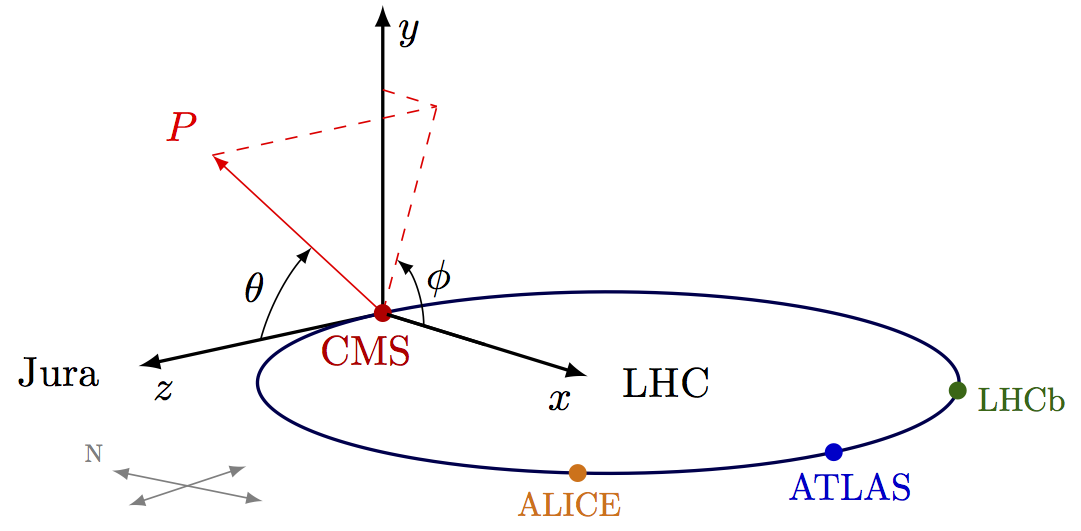
\includegraphics[width=0.8\textwidth]{Images/coordinatechart.png}
    \captionof{figure}{Coordinate system employed by the CMS experiment (retrieved from~\parencite{cmsplots}).}\label{fig_coordinates}
\end{center}

Throughout this work, phenomenological studies and comparisons are primarily developed in the context of CMS, although several results from ATLAS are also referenced, given the close alignment in sensitivity and scope. Measurements performed at CMS adopt a right-handed coordinate system with its origin at the nominal collision point. The $z$-axis is defined along the beam direction, the $x$-axis points radially inward toward the center of the LHC ring, and the $y$-axis points vertically upward. The azimuthal angle $\phi$ is measured in the transverse ($xy$) plane from the $x$-axis, while the polar angle $\theta$ is measured from the $z$-axis, as shown in Fig.~\ref{fig_coordinates}. Moreover, for kinematic analysis at hadron colliders, the Cartesian coordinate system is often reparameterized into quantities that are more physically meaningful and experimentally convenient as shown in Fig.~\ref{fig_cms_coor}:

\begin{description}
	\item[Pseudo-rapidity] $(\eta)$ Instead of using the polar angle, CMS measurements involve the pseudo-rapidity, defined by
	$$
	\eta=-\ln \left(\tan \frac{\theta}{2}\right)
	$$
	The main advantage of using the pseudo-rapidity is that distributions over it tend to be closer to a uniform distribution than those over the polar angle, see Fig.~\ref{fig_cms_coor}. Furthermore, the difference in pseudo-rapidity is invariant under Lorentz boosts along the beam direction~\parencite{book:1123430}.
	
	\item[Transverse Momentum] ($p_T$) Refers to the component of momentum which is perpendicular to the beam line. It is usually preferred over full momentum because momentum along the beamline may just be left over from the beam particles, while the transverse momentum is always associated with whatever physics happened at the vertex, see Fig.~\ref{fig_cms_coor}.
	
	\item[Azimuthal Angle] ($\phi$) Measures the angle in the transverse plane relative to the $x$-axis, providing the directional component perpendicular to the beam line.
\end{description}

\begin{center}
  		% CMS detector - left perspective
		\tdplotsetmaincoords{75}{50} % to reset previous setting
		\begin{tikzpicture}[scale=2.6,tdplot_main_coords,rotate around x=90]
			
			% VARIABLES
			\def\rvec{\L/2/cos(\thetavec)}
			\def\thetavec{18}
			\def\phivec{60}
			\def\L{3.3}    % detector length
			\def\R{0.75}   % detector cylinder radius
			\def\l{4.3}    % beam pipe length
			\def\r{0.04}   % beam pipe radius
			\def\rt{0.042} % beam pipe radius + line thickness
			\def\xmax{1}   % maximum x axis
			\def\ymax{1}   % maximum y axis
			\def\zmin{-\l/2-0.2} % minimum z axis
			\def\zmax{\l/2+0.3}  % maximum z axis
			\def\w{0.3}
			\coordinate (O) at (0,0,0);
			\coordinate (Z) at (0,0,\L/2);
			\tdplotsetcoord{O'}{0.022}{\thetavec}{\phivec} % slightly shifted origin
			\tdplotsetcoord{O''}{0.018}{90}{\phivec} % slightly shifted origin
			\tdplotsetcoord{P}{\rvec}{\thetavec}{\phivec}
			
			% CYLINDER behind
			\def\ang{19} % rotate lines to simulate cylinder
			\fill[top color=red!50!black!4,bottom color=red!60!black!2,rotate around z=\ang]
			(0,\R,\L/2) --++ (0,0,-\L) arc(90:270:\R) --++ (0,0,\L) arc(270:90:\R) -- cycle;
			\fill[detector surface] % transverse plane at z=L/2
			(0,0,\L/2) --++ (0,\R,0) arc(90:270:\R) -- cycle;
			\fill[detector surface] % transverse plane at z=-L/2
			(0,0,-\L/2) --++ (0,\R,0) arc(90:270:\R) -- cycle;
			\tdplotdrawarc[detector]{(0,0,\L/2)}{\R}{0}{360}{}{}
			\tdplotdrawarc[detector,thin]{(0,0,-\L/2)}{\R}{0}{360}{}{}
			%\draw[detector,canvas is yx plane at z=-\L/2] (0,0,0) circle(\R);
			\draw[detector,thin, dashed] % transverse plane at z=0
			(90-\ang:\R) arc (90-\ang:270:\R);
			\draw[detector] (0,0,-\L/2)++(90:\R) --++ (0,0,\L); % top horizontal
			\draw[detector] (0,0,-\L/2)++(-90:\R) --++ (0,0,\L); % bottom horizontal
			
			% BEAM PIPE
			\tdplotdrawarc[beam pipe]{(0,0,\l/2)}{\r}{0}{360}{}{}
			%\tdplotdrawarc[beam pipe]{(0,0,-\l/2)}{\r}{\ang-90}{90}{}{}
			%\draw[beam pipe] % cylindric beam pipe
			%  (0,\r,-\l/2) --++ (0,0,\l) arc(90:-90:\r)
			%  --++ (0,0,-\l) arc(-90:90:\r);
			\draw[beam pipe] % beam pipe, thinner in middle
			(0,\r,-\l/2) -- (0,\r,-0.2*\l) -- (90:0.5*\r)
			-- (0,\r,0.2*\l) -- (0,\r,0.5*\l) arc(90:-90:\r)
			-- (0,-\r,0.2*\l) -- (-90:0.5*\r) --
			(0,-\r,-0.2*\l) -- (0,-\r,-\l/2) arc(-90:90:\r);
			\draw[beam pipe] (0,0,\l/2) circle(\r);
			
			% AXES
			%\draw[thick,->] (0,0,0) -- (0,0,1) node[below right]{$z$}; % short
			\draw[axis,-] (0,0,\zmin) -- (0,0,0); % long
			\fill[CMScol] (O) circle(0.5pt) node[right=1,below=1] {IP};
			\draw[axis] (0,0,0.020) -- (0,0,\zmax) node[right=3,above=0.1]{$z$}; % long
			\draw[axis] (0,0.019,0) -- (0,\ymax,0) node[below left]{$y$};
			\draw[axis] (0.022,0,0) -- (\xmax,0,0) node[below=1,right=-2]{$x$};
			
			% LABELS
			\node[mydarkred,above] at (0,\ymax,0) {$\eta=0$};
			\node[mydarkred,above=0.6, left] at (0,\R,0.3*\L) {$\eta>0$};
			\node[mydarkred,above=0.7, right] at (0,\R,-0.2*\L) {$\eta<0$};
			\node[mydarkred,below=1,left] at (0,0,\zmax) {$\eta=\infty$};
			\node[mydarkred,above=1,right] at (0,0,\zmin) {$\eta=-\infty$};
			
			% VECTORS
			%\fill[radius=0.4,red] (P) circle;
			\draw[dashed,myred] (P)  -- (Pxy);
			\draw[dashed,myred] (Py) -- (Pxy);
			\draw[dashed,myred] (P) -- (Pz);
			
			
			\draw[->,miverde,line cap=round,draw opacity=0.9] (O') -- (P) node[anchor=-30] {\contour{white}{$\va*{p}$}};
			\draw[->,miverde,line cap=round] (O') -- (P) node[anchor=-30] {$\va*{p}$};
			
			\draw[->,azulF,line cap=round,draw opacity=0.9] (O') -- (Pxy) node[right, anchor=-100] {\contour{white}{$\va*{p}_T$}};
			% \draw[->,azulF,line cap=round] (O') -- (Pxy) node[right , anchor=-100] {$\va*{p}_T$};
			
			
			% CYLINDER front
			\draw[beam pipe,fill=none] (0,\r,-\l/2) arc(90:-90:\r);
			\fill[detector surface] % transverse plane at z=L/2
			(0,\rt,\L/2) --++ (0,\R-\rt,0) arc(90:-90:\R) --++ (0,\R-\rt,0) arc(-90:90:\rt);
			\fill[detector surface] % transverse plane at z=-L/2
			(0,\rt,-\L/2) --++ (0,\R-\rt,0) arc(90:-90:\R) --++ (0,\R-\rt,0) arc(-90:90:\rt);
			\tdplotdrawarc[detector]{(0,0,\L/2)}{\R}{-90}{90}{}{} % transverse plane at z=L/2
			\tdplotdrawarc[detector]{(0,0,-\L/2)}{\R}{-90}{90}{}{} % transverse plane at z=-L/2
			\draw[beam pipe,fill=none] (0,\r,\l/2) arc(90:-90:\r);
			\draw[detector,very thin, dashed] % transverse plane at z=0
			(90-\ang:\R) arc (90-\ang:-90:\R);
			
			% ANGLES
			\tdplotdrawarc[thick,red!57!black!3] % contour
			{(O)}{0.2}{4}{0.7*\phivec}{}{}

			% white to contour
			\tdplotdrawarc[draw=azulF, line width=0.6pt, draw opacity=0.9]{(O)}{0.2}{0}{\phivec}{above=2,right=0.75,anchor=-30,text=black}{\contour{white}{$\phi$}}
			\tdplotdrawarc[->, azulF]{(O)}{0.2}{0}{\phivec}{above=2,right=0.75,anchor=-30}{$\phi$}


			\tdplotdrawarc[->,rotate around z=\phivec-90,rotate around y=-90]
			{(O)}{0.88}{0}{\thetavec}{anchor=mid east}{$\theta$}
			\tdplotdrawarc[thick,red!58!black!4,rotate around z=\phivec-90,rotate around y=-90] % contour
			{(O)}{0.3}{88}{0.5*(90+\thetavec)}{}{}
			\tdplotdrawarc[-{>[flex'=1]},rotate around z=\phivec-90,rotate around y=-90,line cap=round]
			{(O)}{0.3}{90}{\thetavec}{above=4.5,right=0.5,anchor=mid east}{$\eta$}
			\draw[mydarkred] (0,0,\L/2) --++ (\R,0,0);
			\tdplotdrawarc[thick,red!60!black!6] % contour
			{(Z)}{0.2}{4}{0.7*\phivec}{}{}
			\tdplotdrawarc[draw=none,opacity=0.8]{(Z)}{0.2}{0}{\phivec}{above=2,right=0.7,anchor=-30}{\contour{red!60!black!6}{$\phi$}}
			\tdplotdrawarc[->]{(Z)}{0.2}{0}{\phivec}{above=2,right=0.7,anchor=-30}{$\phi$}
			
			% COMPASS - CMS-ATLAS axis has a ~12° declination (http://googlecompass.com)
			\begin{scope}[shift={(1.1*\R,-\R,0.2*\L)},rotate around y=12]
				\draw[<->,black!50] (-\w,0,0) -- (\w,0,0);
				\draw[<->,black!50] (0,0,-\w) -- (0,0,\w);
				\node[left,black!50,scale=0.6] at (-\w,0,0) {N};
				\node[below=3,left=-2,green!20!black!50,scale=0.6] at (0,0,\w) {Jura};
				%\node[below=1,right,black!50,scale=0.6,align=center] at (\w,0,0) {center of\\the LHC};
				%\node[below=1,right,blue!30!black!50,scale=0.6] at (\w,0,0) {ATLAS};
			\end{scope}
			\draw[->,thick,orange!30!black] (1.4*\w,-\R,-0.1*\L) --++ (2*\w,0,0)
			node[right,scale=0.8,align=center] {center of\\[-1pt]the LHC};
			
		\end{tikzpicture}
  \captionof{figure}{Detailed reparametrization of the coordinate system employed by the CMS experiment (retrieved from~\parencite{cmsplots})}\label{fig_cms_coor}
\end{center}

Together, the triplet $(p_T, \phi, \eta)$ forms a natural coordinate system that fully describes a particle's three-momentum vector at a hadron collider. The full four-momentum $(E, p_x, p_y, p_z)$ can be reconstructed from these quantities, typically supplemented by either the particle's mass hypothesis (for identified particles like electrons or muons) or the energy deposited in the calorimeters (for neutral objects like photons or jets). This $(p_T, \phi, \eta)$ system serves as the fundamental framework for defining physical objects, calculating event variables, and performing analyses at the LHC, providing both experimental convenience and physical insight into the collision dynamics.


A key challenge is isolating the primary hard interaction from the additional concurrent pile-up interactions. This is accomplished by reconstructing distinct interaction vertices along the beam direction and associating charged particles to their point of origin. The ultimate aim of the reconstruction chain is to identify all stable particles produced in the collision and measure their four-momenta, thereby enabling the identification of the underlying fundamental process.

However, the reconstruction is complicated by several factors. The initial state of the colliding protons is not fully known, as they are composite particles made up of quarks and gluons (collectively referred to as partons). The fraction of the proton's momentum carried by each parton is described by parton distribution functions (PDFs), which are determined experimentally. Consequently, the total momentum along the beam axis ($z$) is not balanced on an event-by-event basis. Furthermore, not all particles are stable enough to reach the detector; some decay before being detected, and only their decay products are observed. The design of a collider experiment, illustrated in Fig.~\ref{fig_layers}, is optimized for the identification and energy measurement of the particles produced in high-energy collisions.

\begin{center}
    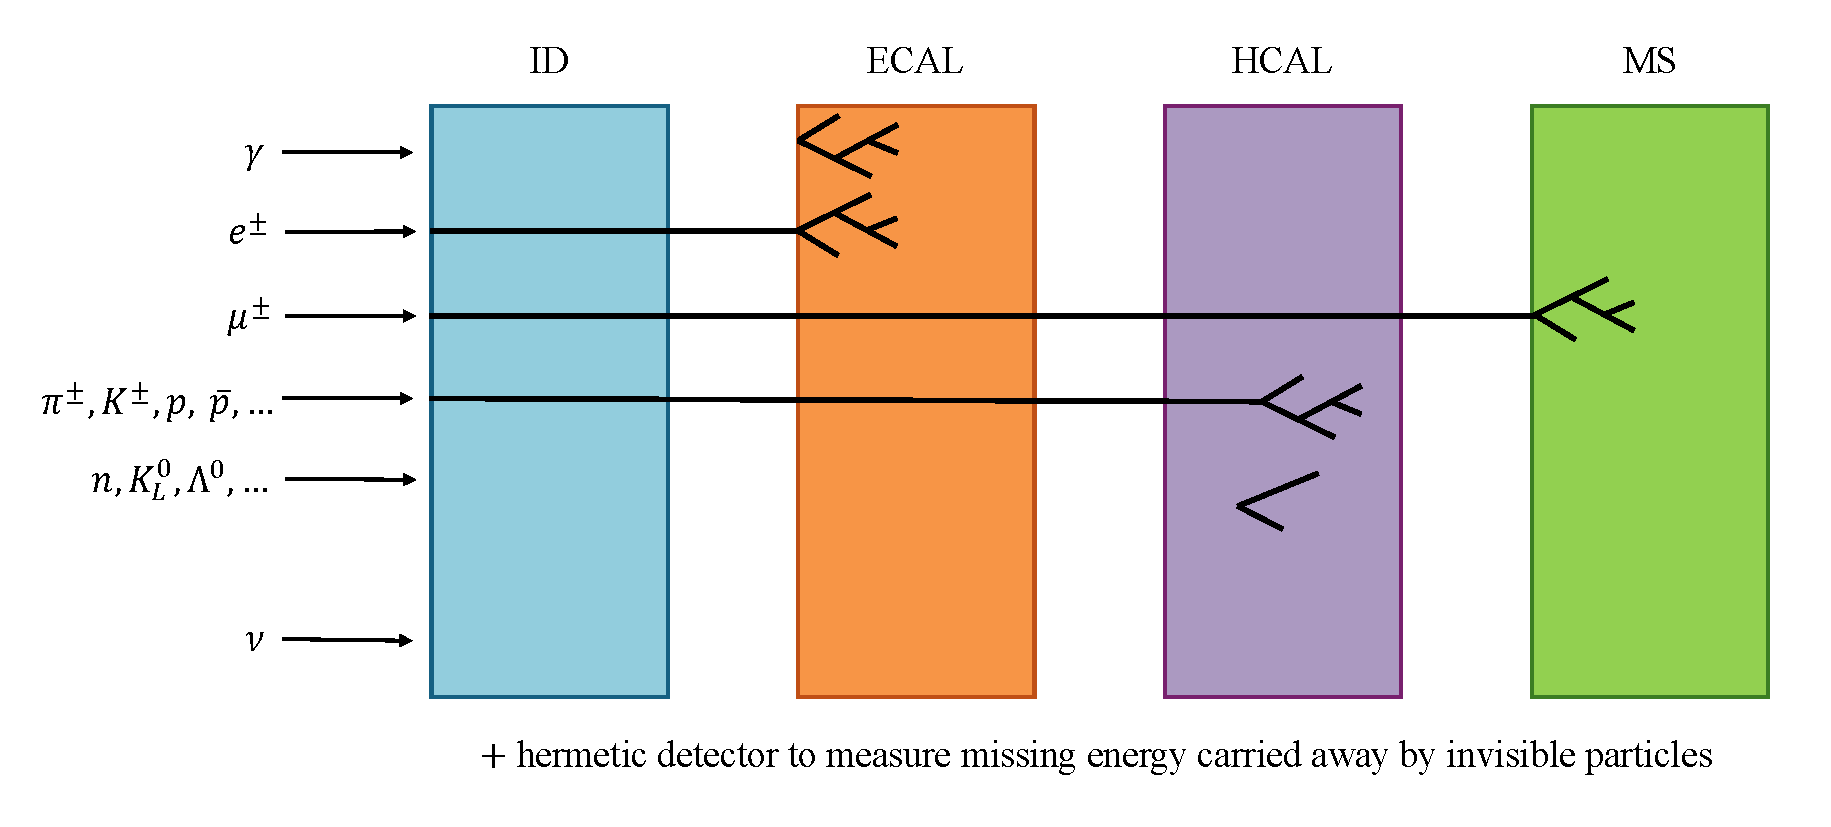
\includegraphics[width=0.95\textwidth]{Images/Layers.pdf}
    \captionof{figure}{Illustration of high-energy particles being identified by consecutive types of subdetectors in a typical collider experiment. The curvature of the tracks in the magnetic field is not shown for simplicity. Representation of which particles and kinds of detectors are used in a multipurpose detector such as CMS or ATLAS.}\label{fig_layers}
\end{center}

Finally, some hypothetical particles, such as those comprising dark matter, along with known neutrinos, interact very weakly with matter and escape direct detection. Therefore, a hermetic detector design is crucial to infer their presence by accurately measuring the imbalance of energy and momentum in the transverse plane, referred to as missing transverse momentum.


In this way, a typical collider experiment comprises several main detector subsystems that are used jointly to detect and measure the properties of particles produced in the collision. A \textit{schematic representation} of such a generic multipurpose detector is shown in Fig.~\ref{fig_detector}. The detector features an "onion-like" design of several concentric layers, each optimized to identify different types of particles and measure their properties.

\begin{center}
    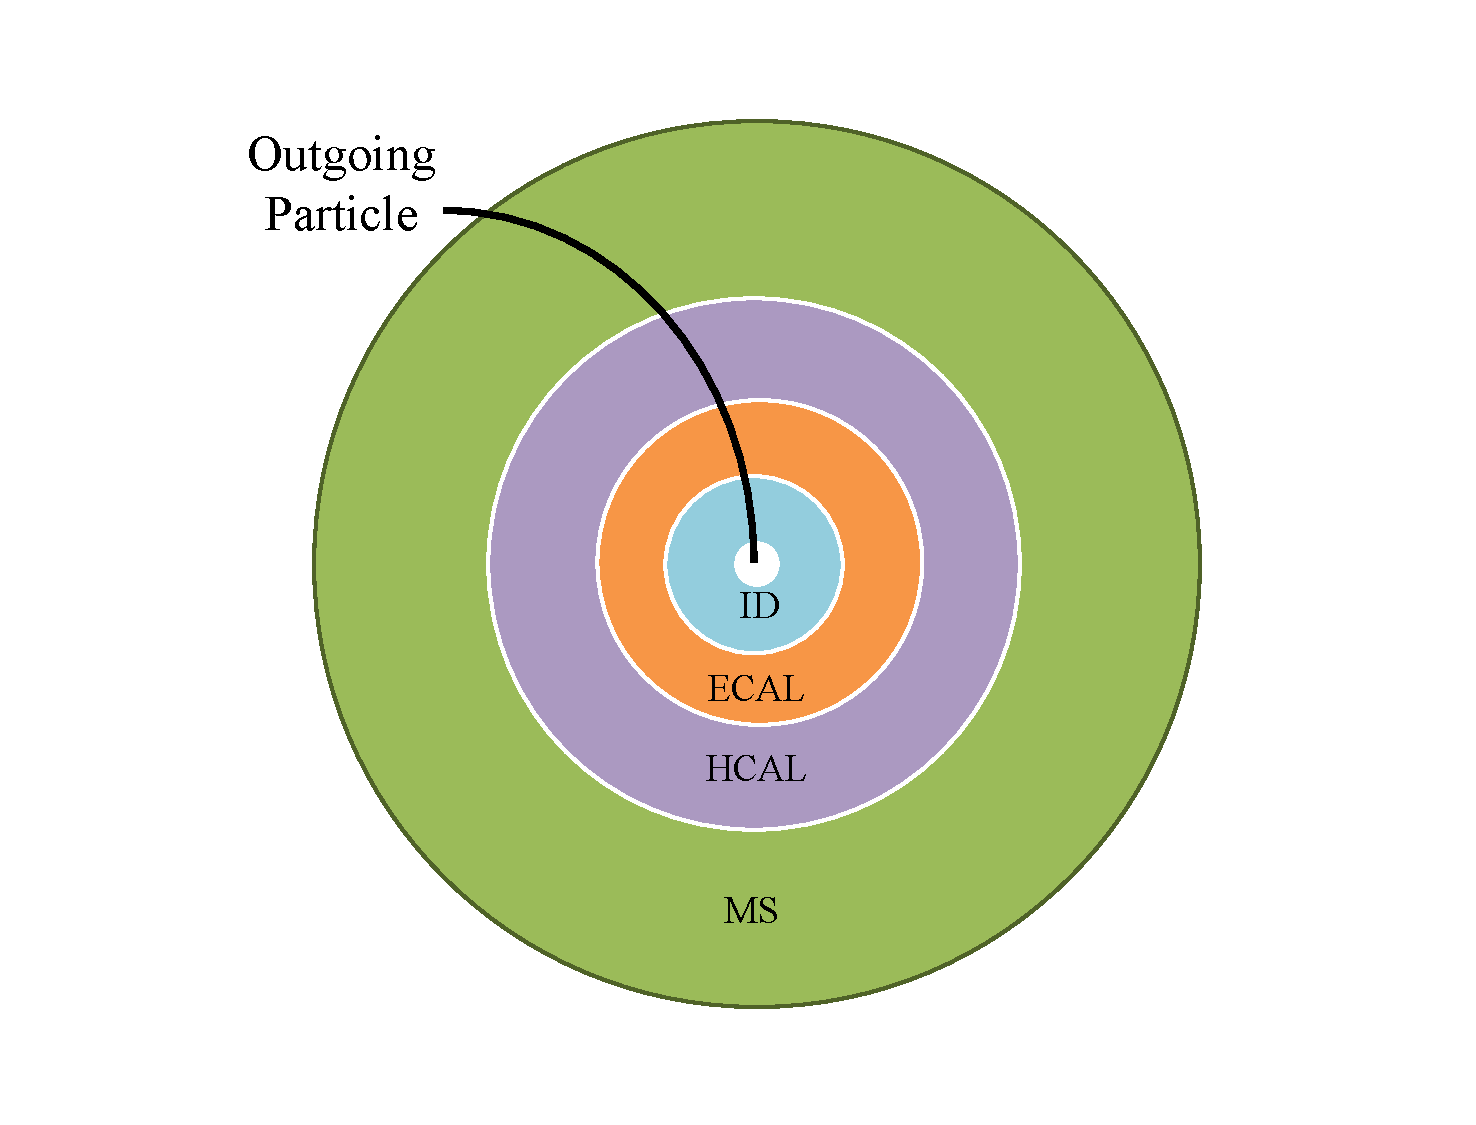
\includegraphics[width=0.8\textwidth]{Images/transversal_detector.pdf}
    \captionof{figure}{Schematic representation of a transverse section of a generic multipurpose detector. The inner detector (ID) is used to measure the trajectories of charged particles, the electromagnetic calorimeter (ECAL) measures the energy of photons and electrons, the hadronic calorimeter (HCAL) measures the energy of hadrons, and the muon system (MS) identifies and measures muons. The missing transverse momentum (MET) is inferred from the momentum imbalance in the transverse plane.}\label{fig_detector}
\end{center}

The innermost subsystem, the inner detector (ID) or tracker, is immersed in a strong axial magnetic field (typically 1–4 T). It is designed to reconstruct the trajectories of charged particles, which are bent by the magnetic field. The direction and curvature of these trajectories, called \textbf{tracks}, yield the particle's momentum vector and electric charge. The most common long-lived charged particles from the SM are leptons (electrons $e$ and muons $\mu$) and hadrons (pions $\pi$, kaons $K$, and protons $p$). In some detectors, the ID is complemented by a Cherenkov-light detector to measure particle velocity. Combined with the momentum measurement, this velocity helps determine the particle mass, allowing for differentiation between pions, kaons, and protons.

After the tracker, particles enter the electromagnetic calorimeter (ECAL), which is designed to fully absorb photons, electrons, and positrons. These particles deposit all their energy in the ECAL by initiating an electromagnetic shower via bremsstrahlung and $e^{+}e^{-}$ pair production. Electrons are identified as charged tracks that point to a compact, high-energy deposit in the ECAL.

The hadronic calorimeter (HCAL) surrounds the ECAL. Its purpose is to absorb hadrons (e.g., neutrons, protons, pions, kaons) and measure their energy through hadronic interactions. High-energy quarks and gluons do not appear as individual particles but instead \textbf{hadronize} into collimated sprays of hadrons known as \textbf{jets}, see Sec.~\ref{sec:jets}. A jet's energy is measured by combining the energy deposited in the ECAL and HCAL with the momenta of charged tracks associated with it. This approach, known as particle flow (PF) reconstruction, provides a more accurate measurement. Neutral hadrons are identified as energy deposits in the calorimeters with no associated track in the ID.

Muons are unique as they are the only charged particles (apart from neutrinos) that can penetrate the entire calorimeter system, losing only a small amount of energy via ionization. Therefore, a dedicated muon system (MS) is built outside the calorimeters. Muons are identified as tracks in the ID that are matched to tracks in the MS. The MS, often within its own magnetic field, provides a standalone momentum measurement, which is combined with the ID measurement for high precision.

Since the detector is nearly hermetic (covering almost the full solid angle), momentum conservation in the plane transverse to the beam line ($x$-$y$ plane) is a powerful tool. The vector sum of the momenta in the transverse plane ($\vec{p}_T$) of all detected particles should be zero. Any significant imbalance indicates the presence of undetected, neutral particles that did not interact with the detector, such as neutrinos or hypothetical new particles. This imbalance is called missing transverse momentum (MET) and is formally defined as:
$$
\vec{p}_T^{\text{miss}} \equiv -\sum_i \vec{p}_{T,i}
$$
where the sum runs over all reconstructed particles (e.g., leptons, photons, jets) or calorimeter deposits in the event.

This sophisticated detector design, optimized for identifying and measuring Standard Model particles, also makes it a powerful instrument for searching for new physics beyond the SM through unusual signatures or an excess of events with large MET.


The event rate $R$ for a physical process (e.g., $pp \to X$) is governed by the accelerator's luminosity $\mathcal{L}$ and the process cross section $\sigma$. Luminosity quantifies the performance of a collider to produce interactions, establishing the proportionality,
\begin{equation}
	\frac{d R}{d t} = \mathcal{L} \sigma,
\end{equation}
where $\sigma$ (typically measured in barns, $1\,\text{b} = 10^{-24}\,\text{cm}^2$) encodes the interaction probability. For LHC proton bunches colliding head-on with Gaussian transverse profiles, the instantaneous luminosity is~\parencite{Herr:941318,book:1123430}:
\begin{equation}
	\mathcal{L} = \frac{f N_{b}}{4\pi} \frac{N_{1} N_{2}}{\sigma_{x} \sigma_{y}}\label{eq_lumi}
\end{equation}
Here, $N_{1,2}$ are proton counts per bunch, $f$ is the bunch collision frequency, $N_{b}$ is the number of bunches, and $\sigma_{x,y}$ are transverse beam widths. 

Integrating $\mathcal{L}$ over time yields the total integrated luminosity $L$, linking directly to the observed event count $N$:
\begin{equation}
	L = \int \mathcal{L}\, dt \quad \Rightarrow \quad N = L \sigma.
\end{equation}

%This major upgrade aims to increase the integrated luminosity by more than an order of magnitude, targeting up to $3\,\mathrm{ab}^{-1}$ of data per experiment. The HL-LHC will significantly enhance the sensitivity to rare processes, improve the precision of Standard Model measurements, and boost the discovery potential for BSM phenomena.

  
The Gaussian beam approximation in~\eqref{eq_lumi} ignores hourglass effects (beam divergence near interaction points) and dynamic $\sigma_{x,y}$ variations during fills. CMS mitigates these via real-time luminosity monitoring using pixel clusters~\parencite{Sirunyan2021}, with systematic uncertainties below $2\%$. High $\mathcal{L}$ also introduces pileup—multiple $pp$ interactions per bunch crossing—which complicates $\eta$/$\phi$ measurements but is corrected using vertex isolation algorithms.


The following variables are related to the particles being produced rather than the accelerator.
\begin{description}
	\item[Decay width] ( $\Gamma)$ The decay rate is the probability that a given particle will decay per unit time. Since a particle can have multiple decay modes, the total decay rate is the sum of the decay rates for each mode~\parencite{book:1123430}. The relative frequency of a decay mode is the branching ratio, given by
	$$
	\mathrm{BR}(j)=\frac{\Gamma(j)}{\Gamma} .
	$$
	\item[Cross-section] $(\sigma)$ The cross-section is a measure of the probability that an interaction will occur from a collision. It is a quantum-mechanical analogue of the "effective size" of the particles involved in an interaction.

	\item[Pseudo-rapidity] $(\eta)$ Instead of using the polar angle, CMS measurements involve the pseudo-rapidity, defined by
	$$
	\eta=-\ln \left(\tan \frac{\theta}{2}\right)
	$$
	The main advantage of using the pseudo-rapidity is that distributions over it tend to be closer to a uniform distribution than those over the polar angle, see Fig.~\ref{fig_cms_coor}. Furthermore, the difference in pseudo-rapidity is invariant under Lorentz boosts along the beam direction~\parencite{book:1123430}.
	\item[Transverse Momentum] ($p_T$) Refers to the component of momentum which is perpendicular to the beam line. It is usually preferred over full momentum because momentum along the beamline may just be left over from the beam particles, while the transverse momentum is always associated with whatever physics happened at the vertex, see Fig.~\ref{fig_cms_coor}.
	\item[Missing transverse energy and momentum] $\left(E_{T}^{\text {miss }} \& p_{T}^{\text {miss }}\right)$ Missing energy and momentum refers to the energy and momentum that is not detected but is expected to be there as a consequence of energy conservation and momentum conservation. This momentum is often carried by particles that do not interact electromagnetically or strongly and are therefore difficult to detect~\parencite{book:1123430}. Missing energy and momentum provides an indirect measurement of undetectable particles in hadron colliders such as neutrinos. Missing momentum reconstructions focus on the transverse direction, where total momentum is expected to be zero.
\end{description}

 
\section{Jets Reconstruction}\label{sec:jets}

Quarks and gluons are never observed as free particles because of colour confinement~\cite{Andersson:1983,Webber:1984}. Nevertheless, perturbative QCD treats them as the relevant short-distance degrees of freedom: factorization theorems and asymptotic freedom justify computing hard-scattering matrix elements for incoming and outgoing partons even though QCD becomes non-perturbative at low scales~\cite{Collins:1989}. The strong coupling $\alpha_s$ grows large and effectively ``blows up'' around the confinement scale $\Lambda_{\mathrm{QCD}}$~\cite{1674-1137-40-10-100001}; consequently, something must happen to quarks and gluons before they reach the detector~\cite{Sjostrand:2014zea}. In practice, the gluon and all quarks except the top hadronize, producing cascades of baryons and mesons that themselves undergo further decays; hadronization is modelled e.g. with the Lund string or cluster models~\cite{Andersson:1983,Webber:1984,Sjostrand:2014zea}. At the LHC, these hadrons typically carry energies comparable to the electroweak scale, and relativistic boosts tend to collimate their decay products into narrow bunches~\cite{Salam:2010}. Those collimated collections of hadrons are the jets we measure at hadron colliders and the objects we use to infer the partons produced in the hard interaction~\cite{Salam:2010,Cacciari:2008gp}.

Each high-energy parton produced in a collision, such as a quark from the process $gg \rightarrow q\bar{q}$, undergoes hadronization over a distance scale of~$\sim10^{-15}\,\mathrm{m}$, producing a jet of hadrons~\cite{Andersson:1983,Sjostrand:2014zea}. The energy composition of these jets is phenomenologically well established and is the basis of particle‑flow reconstruction: on average roughly $\sim60\%$ of the jet energy is carried by charged particles (mostly $\pi^{\pm}, K^{\pm}$), $\sim30\%$ by photons (from $\pi^0\to\gamma\gamma$) and $\sim10\%$ by neutral hadrons~\cite{CMS:PF2017}. In high-energy jets, the particles can be too collimated to be resolved individually in coarse calorimeter segmentation; nevertheless, the jet four‑momentum is reconstructed from clustered PF candidates or calorimeter deposits and then corrected using jet energy corrections derived from simulation and in‑situ data~\cite{CMS:PF2017,Cacciari:2011ma,deFavereau:2013fsa}.

Phenomenologically one usually assumes that each high-energy parton yields a jet and that the measured jet four-momentum can, to useful accuracy, be related to the original parton four-momentum~\cite{Catani:1993,Ellis:1993}. Jets are therefore defined operationally using recombination (clustering) algorithms such as Cambridge–Aachen~\cite{Dokshitzer:1997} or the (anti‑)kT family~\cite{Cacciari:2008gp}. Experimentally this means grouping a large number of energy depositions (or particle‑flow candidates) observed in the calorimeters and tracker into a much smaller set of jets or sub‑jets~\cite{CMS:PF2017}. Nothing in the raw detector data, however, indicates a priori how many jets there should be: the clustering procedure and the choice of a resolution scale fix the outcome~\cite{Salam:2010}. In practice one must either specify the desired number of final jets or choose a resolution/stop criterion (for example a distance parameter $R$, a clustering distance cut, or a jet‑mass/sub‑jet‑resolution threshold) that determines the smallest substructure to be considered a separate parton‑like object~\cite{Thaler:2011}.

Modern reconstruction at the LHC typically uses particle‑flow (PF) candidates as input together with infrared‑ and collinear‑safe clustering algorithms to define jet four‑momenta~\cite{CMS:PF2017,Cacciari:2011ma}. The anti‑$k_T$ algorithm~\cite{Cacciari:2008gp}, implemented in \texttt{FastJet}~\cite{Cacciari:2011ma}, is widely used in ATLAS and CMS; it groups candidates by proximity in the rapidity–azimuth $(y,\phi)$ plane with a typical distance parameter $R\sim0.4$–0.6 and is relatively insensitive to soft radiation and pileup when combined with area‑based subtraction techniques~\cite{Cacciari:2008area}. After clustering, jet energy corrections (JEC) derived from simulation and in‑situ calibrations compensate for detector response, pileup, and underlying‑event effects~\cite{CMS:JEC}, while jet‑substructure and tagging algorithms (mass‑drop, N‑subjettiness, SoftDrop, etc.) help infer the flavour and origin of the initiating parton~\cite{Butterworth:2008,Thaler:2011,Larkoski:2014}.


\subsection{Jet algorithms}

Recombination (or sequential clustering) algorithms formalise the intuitive idea that parton showering produces collinear and soft splittings~\cite{Catani:1993,Dokshitzer:1997,Salam:2010}: two nearby and kinematically compatible sub-jets are merged if they are more likely to have originated from a single parton~\cite{Catani:1993,Dokshitzer:1997}. A practical implementation requires a measure of ``distance'' between objects~\cite{Catani:1993,Cacciari:2011ma}; common choices combine an angular separation in the rapidity–azimuth plane, $\Delta R_{ij}$, with a transverse-momentum weighting~\cite{Catani:1993,Cacciari:2008gp}. Typical distance measures are~\cite{Catani:1993,Dokshitzer:1997,Cacciari:2008gp}
\begin{equation}
  \begin{array}{lll}
  k_T: & y_{ij}=\dfrac{\Delta R_{ij}}{R}\min(p_{T,i},p_{T,j}), & y_{iB}=p_{T,i},\\[6pt]
  \mathrm{C/A}: & y_{ij}=\dfrac{\Delta R_{ij}}{R}, & y_{iB}=1,\\[6pt]
  \text{anti-}k_T: & y_{ij}=\dfrac{\Delta R_{ij}}{R}\min(p_{T,i}^{-1},p_{T,j}^{-1}), & y_{iB}=p_{T,i}^{-1}.
  \end{array}  
\end{equation}
The parameter $R$ balances jet–jet and jet–beam criteria and sets the geometric size of jets; in LHC analyses, typical values are $R\sim0.4\text{--}0.7$ depending on the physics target~\cite{Cacciari:2011ma}.

Two operational modes are useful to distinguish. In an exclusive algorithm, one supplies a resolution scale $y_{\text{cut}}$ and proceeds iteratively:
\begin{enumerate}
  \item compute $y^{\min}=\min_{i,j}\{y_{ij},y_{iB}\}$;
  \item if $y^{\min}=y_{ij}<y_{\text{cut}}$ merge $i$ and $j$ and repeat;
  \item if $y^{\min}=y_{iB}<y_{\text{cut}}$ remove $i$ as beam radiation and repeat;
  \item stop when $y^{\min}>y_{\text{cut}}$ and keep remaining sub-jets as jets.
\end{enumerate}
An inclusive algorithm omits $y_{\text{cut}}$ and instead declares a sub-jet a final-state jet when its jet–beam distance is the smallest quantity; iteration continues until no inputs remain. Inclusive algorithms therefore produce a variable number of jets, while exclusive algorithms deliver a scale-dependent fixed set.

A practical question is how to combine the kinematics of merged objects. The most common choice in modern experiments is the E-scheme: four-vectors are added, which preserves energy–momentum and yields a physical jet mass useful for substructure and boosted-object tagging. An alternative is to sum three-momenta and rescale the energy to enforce a massless jet; this can be appropriate when the analysis targets massless parton kinematics, but it discards potentially useful jet-mass information.

From a theoretical and experimental viewpoint, important properties are infrared and collinear safety: a jet algorithm should give stable results under the emission of soft particles or collinear splittings. The $k_T$, C/A and anti-$k_T$ families are constructed to satisfy these requirements. Their practical behavior differs: $k_T$ naturally follows the physical shower history soft-first clustering, C/A is purely geometric useful for declustering and substructure studies, while anti-$k_T$ produces regular, cone-like jets that are robust and convenient experimentally.

Corrections for pileup and the underlying event are necessary at the LHC. These corrections depend on the jet area and are typically performed by estimating an event-wide transverse-momentum density and subtracting the corresponding contribution proportional to the jet area. Finally, because inclusive algorithms can produce jets arbitrarily close to the beam, a minimum jet $p_T$ threshold, commonly 20–100 GeV depending on the analysis, is imposed to ensure experimental observability and theoretical control.

\subsection{$\tau$ Tagging at Multipurpose Detectors}

The $\tau$ lepton decays hadronically with a probability of $\sim65\%$, producing a narrow ``$\tau$-jet'' that contains only a few charged and neutral hadrons~\cite{1674-1137-40-10-100001,CMS:2018jrd}. Hadronic decays are dominated by one- and three-prong topologies and often include neutral pions that promptly convert to photons, giving a sizable electromagnetic fraction in the calorimeters~\cite{1674-1137-40-10-100001,ATLAS:2014rzk}. When the $\tau$ momentum is large compared to its mass the decay products are highly collimated~\cite{CMS:2018jrd,CMS_DeepTau}: for $p_T>50\ \mathrm{GeV}$ roughly $90\%$ of the visible energy is contained within a cone of radius $R=\sqrt{(\Delta\eta)^2+(\Delta\varphi)^2}=0.2$~\cite{CMS:2018jrd}. These properties motivate the use of small signal cones and narrow isolation annuli in reconstruction~\cite{CMS:2018jrd,CMS_DeepTau}.

Identification exploits three complementary classes of observables~\cite{CMS:2018jrd,ATLAS:2014rzk,CMS_DeepTau,CMS:PF2017}:

\begin{itemize}
  \item Calorimetric isolation and shower-shape variables~\cite{CMS:2018jrd,ATLAS:2014rzk}: hadronic $\tau$ decays deposit localized energy in ECAL+HCAL~\cite{CMS:2018jrd}. Experiments use isolation sums and shape ratios to quantify peripheral activity~\cite{CMS:2018jrd,ATLAS:2014rzk}. Example variables are
  \begin{equation}
    \Delta E_T^{12}=\frac{\sum_{\;0.1<\Delta R<0.2} E_{T,j}}{\sum_{\;\Delta R<0.4} E_{T,i}},\;\;
    P_{\mathrm{ISOL}}=\sum_{\Delta R<0.40}E_T - \sum_{\Delta R<0.13}E_T,
  \end{equation}
  which suppress QCD jets that populate the isolation ring~\cite{CMS:2018jrd}.
  \item Charged-track isolation and prong topology~\cite{CMS:2018jrd,CMS:PF2017}: the few, collimated charged tracks of a $\tau$ allow powerful selections. A common procedure defines a matching cone of radius $R_{\mathrm{m}}$ around the calorimeter jet axis to select candidate tracks above a $p_T^{\min}$ threshold; the leading track (tr$_1$) defines a narrow signal cone $R_{\mathrm{S}}$ (1- or 3-prong hypotheses) and a larger isolation cone $R_{\mathrm{I}}$ is scanned for additional tracks~\cite{CMS:2018jrd,CMS:PF2017}.
  \item Lifetime and vertexing observables~\cite{CMS:TRK2014,1674-1137-40-10-100001}: the finite $\tau$ lifetime ($c\tau\approx87\ \mu\mathrm{m}$) produces displaced tracks and, for multi-prong decays, a reconstructible secondary vertex; impact-parameter significances and secondary-vertex properties are exploited to separate genuine $\tau_h$ from prompt jets or leptons~\cite{CMS:TRK2014,1674-1137-40-10-100001}.
\end{itemize}


Additional discriminants include the invariant mass of the visible decay products computed from tracks and calorimeter clusters, electromagnetic energy fractions (sensitive to $\pi^0\to\gamma\gamma$), and dedicated shower-strip grouping for nearby photons. For example, invariant-mass reconstruction commonly uses a jet cone $\Delta R_{\text{jet}}\lesssim0.4$ while excluding calorimeter clusters matched to tracks by a minimum separation $\Delta R_{\text{track}}\gtrsim0.08$ to reduce double counting.

Reconstruction algorithms combine these inputs. CMS's Hadron-Plus-Strips (HPS) and modern DeepTau methods explicitly build decay-mode hypotheses and use strip-clustering of photons plus multivariate or deep-learning discriminators to reject jets, electrons, and muons~\parencite{CMS:2022ydz,CMS_DeepTau}. ATLAS employs analogous calorimeter+track based MVAs and BDTs~\parencite{ATLAS:2022fgo}. Typical working points trade efficiency versus background: medium points often give $\tau_{\mathrm{h}}$ efficiencies of order 50–70\% with light-jet misidentification rates in the per-mille to percent range, depending on kinematics and pileup.

Practical implementations tune cone sizes, isolation thresholds, and MVA inputs to the kinematic region and analysis goals; the choice of working point is driven by the signal-to-background optimization for the search or measurement at hand.


\subsection{B Tagging at Multipurpose Detectors}

Jets originating from bottom quarks ($b$-jets) exhibit several distinctive properties that enable their identification. The relatively long lifetime of $b$ hadrons (order 1.5 ps) produces displaced charged tracks and often reconstructible secondary vertices a few millimetres from the primary interaction point. The large $b$-hadron mass yields decay products with sizable transverse momentum relative to the jet axis, and semileptonic branching fractions produce soft electrons or muons inside the jet. These features form the basis for $b$-tagging~\cite{CMS_BTV2016}.

Practical algorithms exploit individual signatures or combine them:
\begin{itemize}
  \item \textbf{Track-counting:} counts tracks with large impact-parameter significance to identify a $b$-like topology~\cite{CMS_BTV2016}.
  \item \textbf{Jet-probability:} evaluates the compatibility of the jet's track impact-parameter distribution with the primary vertex hypothesis~\cite{CMS_BTV2016}.
  \item \textbf{Secondary-vertex:} explicitly reconstructs displaced vertices and uses their kinematic properties (decay length significance, vertex mass)~\cite{CMS_BTV2016}.
  \item \textbf{Soft-lepton taggers:} identify low-$p_T$ leptons inside jets from semileptonic $b$ decays~\cite{CMS_BTV2016}.
\end{itemize}

Modern taggers combine many observables in multivariate or deep learning classifiers to maximize discrimination power. Contemporary approaches exploit rich, low level inputs (track by track and PF candidate information, vertex features and kinematics) and advanced network architectures (DeepCSV/DeepJet, RNN/sequence, graph/set networks)~\cite{CMS_BTV2016,Bols_2020,ATLAS:2022fgo}. These developments yield measurable performance gains: modern deep classifiers typically improve $b$ efficiency at fixed mistag rate relative to classical taggers, and allow continuous discriminants with tunable operating points. Calibration with data-driven scale factors (from $t\bar t$, multijet or dilepton control samples) and propagation of associated systematic uncertainties remain essential for physics results~\cite{CMS_BTV2016}.


\begin{itemize}
  \item Deep feed-forward networks (e.g. DeepCSV/DeepJet) ingest a large set of high-level and per-track inputs to produce powerful binary or multi-class discriminants that separate $b$, $c$ and light-flavour jets.
  \item Sequence models and recurrent networks (RNN-based taggers) process an arbitrary ordered list of track-level variables, improving sensitivity by directly exploiting per-track correlations and order-dependent information (impact-parameter sequences, track kinematics).
  \item Graph- and set-based architectures and combined particle+vertex networks (sometimes referred to as ``DeepFlavour''-style models) aggregate heterogeneous inputs and return per-flavour probabilities, enabling natural multi-classification and calibrated operating points.
\end{itemize}

These developments yield measurable performance gains: modern deep classifiers typically improve $b$ efficiency at fixed mistag rate (or reduce mistag rates at fixed efficiency) relative to classical taggers. The continuous output of such networks permits analyses to choose operating points (loose/medium/tight) corresponding to desired efficiencies or mistag targets. Calibration remains essential: data-driven scale factors derived from control samples (e.g. $t\bar t$, multijet, dilepton) are applied to correct simulation, and systematic uncertainties from the calibration, flavour composition, and kinematic extrapolation are propagated to physics results.

Examples in use are CMS DeepCSV / DeepJet and ATLAS MV2 / DL1~\parencite{CMS_DeepTau,ATLAS:2022fgo}, which illustrate the transition from expert-designed high-level variables to large-scale machine learning leveraging low-level detector information. Typical medium working points yield $b$-tag efficiencies of order 60–80\% with light-jet misidentification rates at or below the percent level; the precise choice of working point is tuned per analysis to optimise sensitivity while accounting for calibration and systematic uncertainties.

\section{The CMS Detector}

CMS is a general-purpose detector at the LHC~\parencite{CMS_2008}. With a length of 21.6~m, a diameter of 14.6~m, and a weight of 14,000 tonnes, its cylindrical geometry is divided into a central barrel section and two endcaps. This design provides hermetic coverage to accurately measure momentum and energy balance, which is crucial for identifying non-interacting particles like neutrinos through missing transverse energy.



The detector is constructed from concentric layers of sub-detectors, as illustrated in Figure~\ref{fig_cms}. The innermost component is the silicon tracker, comprising a pixel detector and silicon strip tracker. It reconstructs the trajectories of charged particles and measures their transverse momenta ($p_T$) with a resolution of $\approx 0.7\%$ for 10~GeV particles within a pseudorapidity range of $|\eta| < 2.5$.

Surrounding the tracker is the calorimetric system. The electromagnetic calorimeter (ECAL) is made of lead-tungstate crystals. It is designed to measure electrons and photons with a high resolution of $\approx 0.6\%$ for 50~GeV electrons. The hadronic calorimeter (HCAL), located outside the ECAL, is a brass-scintillator sampling calorimeter that measures hadrons (e.g., charged pions, kaons, protons) with an energy resolution of $\approx 18\%$ for 50~GeV pions. Together, the ECAL and HCAL cover $|\eta| < 3$. The coverage is extended to $|\eta| < 5$ with steel and quartz-fiber hadron calorimeters in the forward regions.


\begin{center}
	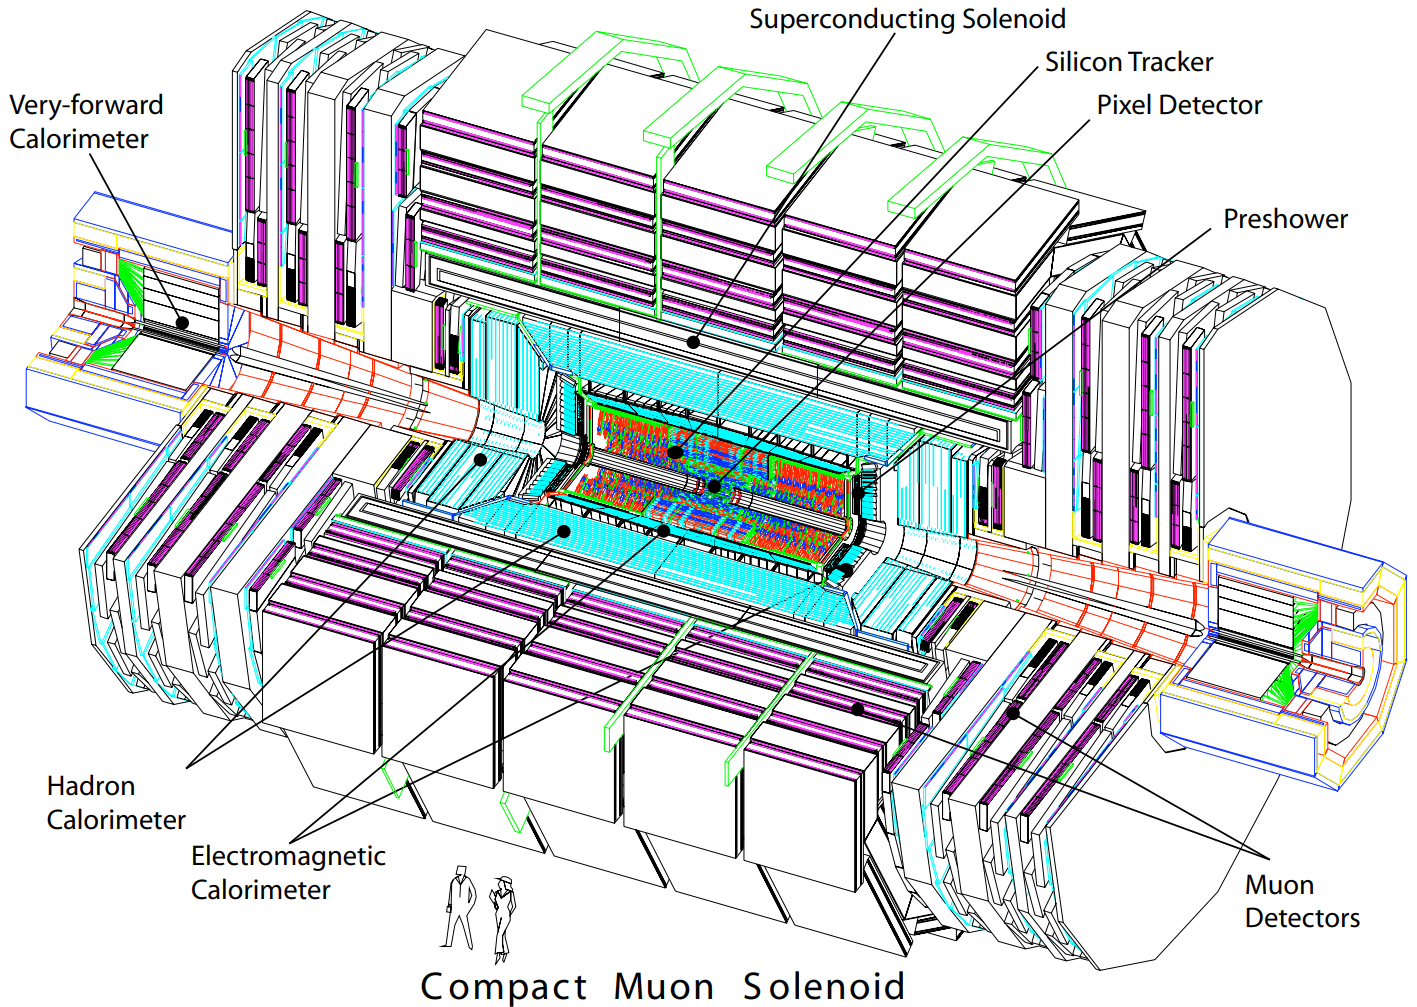
\includegraphics[width=0.9\textwidth]{Images/CMS.png}
	\captionof{figure}{Layout of the CMS experiment at the CERN LHC. (retrieved from~\parencite{CMS_2008}).}\label{fig_cms}
\end{center}

A key feature of CMS is its large superconducting solenoid, which encloses the tracker and calorimeters. The solenoid is constructed from a niobium-titanium alloy and cooled to 4.2~K with liquid helium. It generates a uniform magnetic field of 3.8~T throughout the tracking volume, enabling precise momentum measurement from the curvature of charged particle tracks.

The outermost system is dedicated to muon identification and measurement. Gas-ionization detectors are embedded in the steel flux-return yoke that surrounds the solenoid. This system provides triggering and tracking capabilities for muons up to $|\eta| < 2.4$. The combination of the inner tracker and the muon system allows for a robust identification and momentum measurement of muons across a wide kinematic range.

The geometrical segmentation of the barrel and endcaps defines the detector's acceptance in terms of pseudorapidity. The central barrel provides optimal coverage for $|\eta| \lesssim 1.5$, while the endcaps extend the acceptance to $|\eta| \lesssim 2.5$ for the tracker and calorimeters, and to $|\eta| \lesssim 2.4$ for the muon system.

This segmentation impacts the detection efficiency. The silicon trackers are highly efficient in the barrel, where particles cross the layers perpendicularly. In the endcaps, the reduced hit multiplicity from shallow-angle traversals leads to a slight decrease in tracking efficiency and resolution. The calorimeters are also optimized to maintain performance across $\eta$, though the material budget and granularity vary.

Muon reconstruction performance exhibits regional differences. In the barrel, drift tubes (DTs) provide high spatial resolution, while in the endcaps, cathode strip chambers (CSCs) and resistive plate chambers (RPCs) are used to handle higher background rates and non-uniform magnetic fields. The assumed identification efficiency for muons (electrons) is 95\% (85\%), with a mis-identification rate of 0.3\% (0.6\%)~\parencite{CMS-PAS-FTR-13-014,CMS_MUON_17001,CMS_EGM_17001}.

For the identification of heavy-flavor jets, we adopt the DeepCSV algorithm~\parencite{CMS_BTV2016}. We use its ``medium'' working point, which provides a $b$-tagging efficiency of 70\% with a light-flavor jet misidentification rate of approximately 1\% across the entire $p_T$ spectrum. The ``loose'' (85\% efficiency, 10\% mis-id) and ``tight'' (45\% efficiency, 0.1\% mis-id) working points were also explored during the analysis optimization.

For hadronically decaying $\tau$ leptons ($\tau_h$), we use the DeepTau algorithm~\parencite{CMS_DeepTau}, which employs a deep neural network combining isolation and lifetime information to identify $\tau_h$ decay modes. The ``medium'' working point is chosen for this analysis, providing a $\tau_h$ identification efficiency of 70\% and a misidentification rate of 0.5\% for jets originating from light quarks and gluons. This working point was selected through an optimization process that maximized the discovery reach of the analysis.
 
\section{The Phenomenological Pipeline: From Theory to Observables}

The estimation of signal and background event yields is performed through a comprehensive Monte Carlo (MC) simulation pipeline. This approach, a cornerstone of high-energy physics research, enables robust studies of Beyond the Standard Model (BSM) scenarios by emulating the entire data collection and processing chain of a collider experiment. The key advantages of this methodology include:

\begin{itemize}
    \item The ability to perform automated calculations of theoretical quantities such as cross-sections and decay widths for complex processes.
    \item Conducting feasibility studies and optimizing analysis strategies prior to data acquisition.
    \item Estimating the efficiency of complex event selection criteria and the geometric acceptance of the detector.
    \item Predicting the rates and kinematical distributions of both irreducible and reducible background processes.
    \item Comparing and distinguishing between different theoretical hypotheses for a potential discovered signal.
\end{itemize}

The simulation workflow is modular, reflecting the logical progression from a theoretical Lagrangian to simulated detector-level observables. A schematic view of this pipeline is presented in Figure~\ref{fig:sim_workflow}. The process begins with the implementation of the theoretical model in \texttt{FeynRules} (v2.3.43)~\parencite{Christensen:2008py,Alloul:2013bka}. The Lagrangian of the new physics scenario, including all particle definitions, parameters, and interactions, is translated into a set of Feynman rules. The output is exported in the Universal FeynRules Output (UFO) format, a standard interoperable with modern matrix element generators.

This UFO module, accompanied by a parameter card defining the numerical values of all model parameters (masses, couplings, etc.), serves as input to the \texttt{MadGraph5\_aMC@NLO} (v3.5.7)~\parencite{Alwall:2014bza,Alwall:2014hca} framework. Within MadGraph, the hard scattering process is defined, and the corresponding matrix elements (ME) and Feynman diagrams are generated at leading order (LO) in QCD. For this analysis, proton-proton collisions are simulated at center-of-mass energies of $\sqrt{s}=13 \tev$ and $\sqrt{s}=13.6 \tev$, utilizing the NNPDF3.0 NLO~\parencite{NNPDF:2014otw} set of parton distribution functions (PDFs). This choice is motivated by its global fit accuracy and consistency for both LO and NLO simulations.

To accurately model processes featuring significant interference effects between the new physics signal (e.g., a $\zb'$ boson) and the Standard Model backgrounds, the full squared amplitude (often referred to as the Signal-Discriminated Events or SDE strategy) is employed for the phase-space integration. The \texttt{MadEvent} submodule then generates unweighted parton-level events, which are stored in the Les Houches Event (LHE) format, containing the four-momenta of all final-state particles. The generation is optimized through careful configuration of the \texttt{run\_card}, setting appropriate kinematic cuts on final-state partons to avoid wasting computational resources on events that would subsequently be rejected by the detector simulation.

Given the presence of additional jet radiation, the MLM matching scheme~\parencite{Alwall:2007fs} is applied to mitigate the double-counting of jet emission between the matrix element calculation and the subsequent parton shower. This ensures a smooth transition between the hard process and softer radiative effects.

The parton-level LHE events are then passed to \texttt{PYTHIA} (v8.2.44)~\parencite{Sjostrand:2014zea} for the modeling of QCD and QED radiation (parton showering), hadronization, and particle decays. This step translates the colored partons into stable, color-singlet hadrons and resonances that form the observable final state. The resulting events, which include a full list of generator-level particles, are saved in the HepMC2 format.

Detector effects are simulated using \texttt{DELPHES} (v3.4.2)~\parencite{deFavereau:2013fsa}, a fast parametric detector simulation framework. The \texttt{delphes\_card\_CMS.tcl} configuration card is used to emulate the response of the CMS detector, including the geometric acceptance, tracking efficiency, calorimeter energy resolution and segmentation, and magnetic field. Key reconstruction algorithms are applied within DELPHES:
\begin{itemize}
    \item Jets are clustered from calorimeter towers using the anti-$k_t$ algorithm~\parencite{Cacciari:2008gp} with a distance parameter of $R=0.4$, and $b$-tagging is simulated based on the efficiency and mis-tag rate of the CMS performance.
    \item Muons and electrons are identified with efficiency maps that are functions of $p_T$ and $\eta$.
    \item The missing transverse energy (MET) is calculated from the negative vector sum of all reconstructed particle momenta.
\end{itemize}
The final output, containing reconstructed physics objects (jets, leptons, MET), is stored in ROOT format~\parencite{Brun:1997pa}.

At this stage, the analysis of the simulated samples converges with the methodology applied to real collider data. The subsequent steps involve applying event selection criteria, calibrating and scaling the reconstructed objects (e.g., applying Jet Energy Corrections), and performing statistical interpretation. The reliability of the simulation is validated by comparing the modeling of well-known Standard Model processes (e.g., Drell-Yan, $t\bar{t}$ production) against published results and data-driven control regions. Dominant theoretical systematic uncertainties, such as those arising from the choice of factorization and renormalization scales, PDF variations, and parton shower modeling, are evaluated and propagated through the analysis.

 
\section{Measurement of the Power of an Analysis}
\label{sec:power_analysis}

In high energy physics experiments, data is often discretized into bins (e.g., histograms of collision events versus energy or momentum) to test competing hypotheses~\cite{BakerCousins:1984}. The fundamental framework compares two scenarios: the \textit{null hypothesis} ($H_0$), representing background-only processes (only a $b_i$ number of events in each bin $i$), and the \textit{alternative hypothesis} ($H_1$), including both signal ($s_i$) and background events ($s_i + b_i$)~\cite{NeymanPearson:1933}. Event counts ($n_i$) in a collider experiment follow a Poissonian distribution. Therefore,  the likelihood for observing the data under each hypothesis is the product of Poisson probabilities per bin. And, because of this, it is  written as a binned-likelihood~\cite{BakerCousins:1984,Cowan:2011}:
\begin{equation}
    \mathcal{L}(n_i \mid \lambda_i) = \frac{e^{-\lambda_i} \lambda_i^{n_i}}{n_i!}, \quad \text{where } \lambda_i = 
    \begin{cases}
        b_i & \text{for } H_0, \\
        s_i + b_i & \text{for } H_1.
    \end{cases}
\end{equation}
The Neyman-Pearson lemma~\parencite{NeymanPearson:1933,Segura:2024srj} provides a rigorous framework for hypothesis testing by establishing that the \textit{likelihood ratio} $Q = \mathcal{L}(\text{data} \mid H_1)/\mathcal{L}(\text{data} \mid H_0)$ is the most powerful test statistic for distinguishing between two simple hypotheses, $H_0$ and $H_1$~\cite{NeymanPearson:1933,Cowan:2011}. This forms the basis for quantifying the evidence for new physics signals against known backgrounds~\cite{Cowan:2011,Read:2002}. For binned analyses in particle physics, we define the likelihood ratio $Q_i$ for each bin $i$ as~\cite{BakerCousins:1984,Cowan:2011},
\begin{equation}
Q_i = \frac{\mathcal{L}(n_i \mid s_i + b_i)}{\mathcal{L}(n_i \mid b_i)} = e^{-s_i} \left( 1+\frac{s_i}{b_i} \right)^{n_i},
\end{equation}
where $n_i$ is the observed event count, $s_i$ the expected signal, and $b_i$ the expected background in bin $i$, as explained before~\cite{BakerCousins:1984,Cowan:2011}. 

The test for the full analysis is constructed as the product of individual bin likelihood ratios~\cite{BakerCousins:1984,Cowan:2011}:
\begin{equation}
Q = \prod_{i=1}^{N} Q_i,
\end{equation}
where $N$ is the total number of bins~\cite{BakerCousins:1984}. Under this formulation, each bin is treated as an independent experiment, allowing us to analyze the data in a modular way. This is convenient when combining results from multiple search channels or energy ranges~\cite{Read:2002,Cowan:2011}. 

For convenience and to connect with asymptotic results, one commonly works with the log-likelihood ratio:
\begin{equation}
-2\ln Q = 2\sum_{i=1}^{N}\left[s_i - n_i \ln\left(1 + \frac{s_i}{b_i}\right)\right],
\end{equation}
and, by Wilks' theorem, its asymptotic distribution under the null hypothesis is chi-square distributed in regular cases~\cite{Wilks:1938,Cowan:2011}.

In practice, the Neyman-Pearson lemma motivates the use of a test statistic $t$ that quantifies the evidence for a signal against the background-only hypothesis, which can be written as
\begin{equation}
t=-2\ln Q = \sum_{i=1}^{N} \left[2s_i - 2n_i w_i\right],
\end{equation}
with the optimal weight of each bin given by $w_i = \ln\!\left(1 + \frac{s_i}{b_i}\right)$.




The discovery significance $\kappa$ quantifies the statistical separation of $t$ if $n$ is distributed according to the background-only hypothesis ($H_0$) versus the signal-plus-background hypothesis ($H_1$), normalized by the standard deviation of the $H_1$ distribution ($\sigma_{H_1}$),
\begin{equation}
\kappa = \frac{\braket{t}_{H_0} - \braket{t}_{H_1}}{\sigma_{H_1}}.
\end{equation}
The expected behavior differs under the signal-plus-background ($H_1$) and background-only ($H_0$) hypotheses:

\begin{itemize}
	\item \textbf{Under $H_1$} we expect that the $n_i$ data distribution follows $\text{Pois}(s_i + b_i)$:
	\begin{equation}
	\langle -2\ln Q \rangle_{s+b} = \sum_i \left[2s_i - 2(s_i + b_i)w_i\right]
	\implies \sigma^2_{s+b} = 4\sum_i (s_i + b_i) w_i^2.
	\end{equation}

	\item \textbf{Under $H_0$} we expect that the $n_i$ data distribution follows $\text{Pois}(b_i)$
	\begin{equation}
	\langle -2\ln Q \rangle_{b} = \sum_i \left[2s_i - 2b_i w_i\right]
	\implies \sigma^2_{b} = 4\sum_i b_i w_i^2
	\end{equation}
\end{itemize}
Substituting in $\kappa$ gives a useful expression for the discovery significance,
\begin{align}
\kappa = \frac{\sum s_i w_i}{\sqrt{\sum (s_i + b_i) w_i^2}}
\end{align}
It quantifies the separation between the signal+background ($s+b$) and the background-only hypotheses in units of standard deviations ($\sigma$), where $\kappa = 5$ corresponds to the traditional $5\sigma$ discovery threshold, $\kappa =3$ to a $3\sigma$ evidence to the traditional anomaly detection threshold, and $\kappa = 1.69$ to the $95\%$ confidence level (CL) exclusion limit.


This figure of merit automatically optimizes sensitivity through the logarithmic weights $w_i = \ln(1 + s_i/b_i)$, which naturally emphasize bins with either high signal-to-background ratios ($s_i/b_i$) or large absolute signal contributions ($s_i$). In asymptotic limits, $\kappa$ simplifies to intuitive forms: for dominant signals ($s_i \gg b_i$), it approaches $\sqrt{\sum s_i}$ (Poisson counting), while in background-dominated regimes ($s_i \ll b_i$), it reduces to an inverse-variance-weighted sum $\sum s_i / \sqrt{\sum b_i (s_i/b_i)^2}$. This dual behavior ensures optimal discrimination power across all signal regimes.

In practice, we must take into account systematic effects by incorporating nuisance parameters into the likelihood and profiling over uncertainty ranges. The power calculation can be extended to include systematic uncertainties by modifying the denominator as,
\begin{equation}
	\boxed{
	\kappa_{\text{sys}} = \frac{\sum_i s_i w_i}{\sqrt{\sum_i \left[(s_i + b_i) + \delta^2_{\text{sys,signal},i} + \delta^2_{\text{sys,bkg},i}\right] w_i^2}},
}
\label{eq:kappa_with_systematics}
\end{equation}
where $\delta_{\text{sys}}$ terms represent the systematic uncertainties on signal and background predictions.

This framework not only provides a figure of merit for an analysis but also serves as a roadmap for experimental optimization. The expected signal and background in each bin, $s_i$ and $b_i$, are not fundamental inputs but are themselves products of the experimental setup and analysis choices. They can be expressed in terms of more fundamental experimental parameters (with acceptance absorbed into the selection efficiencies):
\begin{align*}
    s_i &= \sigma_{s,i} \cdot L \cdot \epsilon_{s,i}, \\
    b_i &= \sigma_{b,i} \cdot L \cdot \epsilon_{b,i},
\end{align*}
where, following Equation~\ref{eq:N_sigma_experiment}, $\sigma_{s,i}$ and $\sigma_{b,i}$ are the fiducial cross-sections for signal and background processes in bin $i$, $L$ is the integrated luminosity, and $\epsilon_{s,i}$ and $\epsilon_{b,i}$ are the cumulative or total efficiencies (selection efficiency combined with detector acceptance and reconstruction effects).

Substituting these expressions into the significance $\kappa$ reveals the multidimensional parameter space available for optimization:
\[
\kappa = \frac{\sum_i \sigma_{s,i} \cdot \epsilon_{s,i} \cdot w_i}
{\sqrt{\sum_i \left[ (\sigma_{s,i}\epsilon_{s,i} + \sigma_{b,i}\epsilon_{b,i}) + \delta^2_{\text{sys}} \right] \cdot w_i^2}} \cdot \sqrt{L}.
\]

This decomposition shows that the discovery significance can be enhanced through several distinct strategies. The primary handles are:

\begin{itemize}
    \item \textbf{Increasing integrated luminosity} ($L$): The $\sqrt{L}$ scaling represents the fundamental statistical limit - doubling sensitivity requires quadrupling data collection time. This drives the construction of higher-luminosity colliders and longer data-taking campaigns.
    
    \item \textbf{Reducing systematic uncertainties}: The $\delta_{\text{sys}}$ terms encompass uncertainties from theoretical predictions, detector calibration, background estimation methods, and luminosity measurement. Their reduction requires dedicated calibration measurements, improved Monte Carlo simulations, and sophisticated data-driven background estimation techniques.

		\item \textbf{Improving detector performance}: Effective efficiencies $\epsilon_{s,i}$ and $\epsilon_{b,i}$ can be improved through better detector design, increased coverage, and enhanced reconstruction and calibration algorithms that recover and correctly identify more signal events while controlling backgrounds.

    \item \textbf{Choosing optimal observables}: The weights $w_i = \ln(1 + s_i/b_i)$ are maximized when the analysis uses variables that provide the best separation between signal and background. This motivates the development of advanced feature engineering and the use of multivariate methods that automatically learn the most discriminating variables.

    \item \textbf{Optimizing selection criteria}: Signal efficiency $\epsilon_{s,i}$ can be maximized while background efficiency $\epsilon_{b,i}$ is minimized through sophisticated trigger algorithms, multivariate analysis techniques, and machine learning classifiers that exploit subtle differences between signal and background event features.

\end{itemize}

Therefore, the power of an analysis, quantified by $\kappa$, is the result of a concerted effort across accelerator operation, detector performance, and analysis strategy.

The key limitation of the binned formulation in Eq.~\ref{eq:kappa_with_systematics} is its treatment of bins as independent experiments, which discards valuable information from inter-bin correlations. This approximation becomes particularly evident in regions of high sensitivity, where the shape information of distributions becomes crucial. In such cases, multivariate methods that exploit the full correlation structure (such as matrix element methods, deep learning classifiers, or template fits) typically outperform simple binned significance estimates.

However, the formalism presented here provides theoretical insight and a useful approximation for quick sensitivity estimates. In the asymptotic limit and for counting experiments, this approach yields results consistent with statistical packages commonly used in high energy physics, such as \texttt{RooStats} and \texttt{RooFit}. These frameworks implement more rigorous statistical procedures that fully account for the likelihood structure, parameter correlations, and systematic uncertainties through nuisance parameters.


Despite this limitation, the $\kappa$ metric remains invaluable for establishing \textit{experimental sensitivity}, which is defined as the minimum signal strength required to achieve a certain significance level (e.g., 95\% CL exclusion or $5\sigma$ discovery potential). It provides a practical tool for guiding analysis design, optimizing selection criteria, and prioritizing experimental efforts. 

For experimental final results and interpretation, full statistical treatments using profile likelihood methods within frameworks such as \texttt{RooStats} remain the gold standard, as they properly account for all correlations and systematic uncertainties. In this work, we are not interested in the final statistical interpretation of data, but rather in understanding and optimizing the experimental sensitivity to new physics signals. Therefore, the $\kappa$ metric serves as a practical and insightful tool for guiding analysis design and experimental strategy.
 
\section{Machine Learning in High-Energy Physics: Motivation and Methods}
\label{sec:machine_learning}

As shown in Section~\ref{sec:power_analysis}, the sensitivity of a search depends on optimally separating signal and background processes. We suppose that, traditional cut-based analyses, which apply sequential selection criteria to individual observables, cannot fully exploit the discriminatory information contained in the high-dimensional feature space of collision events. In this approach, for an event described by feature vector $\mathbf{x} = (x_1, x_2, \ldots, x_N)$, we apply sequential cuts in the form
\begin{equation}
\text{Selection:} \quad x_1 > c_1 \,\text{AND}\, x_2 > c_2 \,\text{AND}\, \ldots \,\text{AND}\, x_N > c_N.
\end{equation}

This method has several limitations which become apparent when considering correlations among kinematic variables. A typical LHC event contains a large list of observables and an optimal discriminator must consider all these variables and their relationships simultaneously, we employ machine learning to address this challenge. Hard cut boundaries discard events that are signal-like in multivariate space but fall just outside univariate cuts. And, furthermore, the challenge of dimensionality, as optimizing many cuts becomes unstable and prone to statistical fluctuations. Finally, it cannot capture non-linear relationships and complex decision boundaries that often provide the strongest discrimination.


Particularly, supervised learning addresses these limitations directly. It learns a function $f(\mathbf{x})$ that maps the high-dimensional input space to a continuous score approximating the posterior probability:
\begin{equation}
f: \mathbb{R}^N \rightarrow [0,1], \quad f(\mathbf{x}) \approx P(\text{signal} \mid \mathbf{x}).
\end{equation}
This score incorporates correlations and non-linearities present in the training data, providing a powerful, continuous discriminant.

Formally, the classification problem can be stated as follows. Each collision event is represented by a feature vector $\mathbf{x} = (x_1, x_2, \ldots, x_N)$, where the components correspond to reconstructed kinematic variables or high-level observables. The task is to assign a label
\begin{equation}
y =
\begin{cases}
1 & \text{if the event originates from the signal process}, \\
0 & \text{if the event originates from the background}.
\end{cases}
\end{equation}
Rather than producing a hard label, modern classifiers return a continuous score $f(\mathbf{x}) \in [0,1]$ that estimates the probability of an event being signal given its features. This formulation allows the classifier to exploit multidimensional correlations and complex decision boundaries that cut-based methods cannot capture.

From a machine learning perspective, this is a standard supervised binary classification problem. In high-energy physics, however, its goal is not conventional metrics such as accuracy or precision, but the improvement of search sensitivity. The classifier is an intermediate tool: it provides a discriminant that maximizes the separation of signal and background distributions, which is then used in hypothesis testing and limit setting.

Several algorithms are commonly employed in this context, and their selection depends on the complexity of the feature space, the size of the available training data, and the balance between interpretability and performance. \textit{Logistic regression} is often used as a baseline due to its simplicity and transparency. It assumes a linear decision boundary in the feature space, with the discriminant given by
\begin{equation}
f(\mathbf{x}) = \sigma(\mathbf{w} \cdot \mathbf{x} + b), \quad 
\sigma(z) = \frac{1}{1 + e^{-z}},
\end{equation}
where $\mathbf{w}$ are model parameters and $b$ is a bias term. While it cannot capture complex non-linear relationships, logistic regression remains useful when signal and background are approximately linearly separable, and it provides a clear reference point against which more sophisticated methods can be compared.

\textit{Neural networks} extend classification capability to non-linear decision boundaries by composing layers of affine transformations with non-linear activation functions. A feed-forward neural network with $L$ layers can be written schematically as
\begin{equation}
f(\mathbf{x}) = \sigma^{(L)}\!\left(W^{(L)} \, \sigma^{(L-1)} \!\left( \cdots \sigma^{(1)}(W^{(1)} \mathbf{x} + b^{(1)}) \cdots \right) + b^{(L)} \right).
\end{equation}
This architecture allows the network to approximate highly complex functions of the input variables, making it suitable for capturing correlations that are difficult to model otherwise. In practice, shallow networks have long been employed in collider physics, while larger datasets now permit the exploration of deeper architectures. Their main drawbacks are reduced interpretability and sensitivity to hyperparameter choices.

\textit{Boosted decision trees} (BDTs) have become a standard tool in particle physics because they offer a favorable balance between interpretability and performance. A single decision tree partitions the feature space through binary splits (e.g., ``Is $x_i < \text{threshold}$?'') and assigns class probabilities to terminal nodes. However, an individual tree is a high-variance learner, sensitive to fluctuations in the training data. Boosting addresses this by combining many weak learners (typically shallow trees) into a strong ensemble:
\begin{equation}
F_M(\mathbf{x}) = \sum_{m=1}^{M} \gamma_m h_m(\mathbf{x}),
\end{equation}
where each new tree $h_m(\mathbf{x})$ corrects the errors made by the current ensemble $F_{m-1}(\mathbf{x})$, and $\gamma_m$ is its weight. This sequential correction process produces a powerful classifier. BDTs are robust to outliers and non-Gaussian distributions, naturally handle mixed variable types, and automatically perform feature selection, often revealing which observables carry the most discriminating power. For these reasons, they are widely adopted in LHC analyses as the default multivariate method.


\subsection{XGBoost: Optimized Gradient Boosting}
\label{ssec:xgboost}

The \textit{XGBoost} (eXtreme Gradient Boosting) library is a state-of-the-art implementation of gradient boosting, known for its computational efficiency and performance, making it widely used in high-energy physics. The algorithm optimizes a regularized objective function:
\begin{equation}
\mathcal{L} = \sum_{i=1}^{n} l(y_i, \hat{y}_i) + \sum_{m=1}^{M} \Omega(f_m),
\end{equation}
where $l(y_i, \hat{y}_i)$ is a differentiable loss function and $\Omega(f_m)$ is a regularization term that penalizes tree complexity, reducing overfitting. The model is built additively:
\begin{equation}
\hat{y}_i^{(t)} = \hat{y}_i^{(t-1)} + f_t(\mathbf{x}_i),
\end{equation}
with each $f_t$ chosen to minimize the objective function. XGBoost's advantages include efficient algorithms for finding optimal splits, sophisticated handling of missing data, and integrated cross-validation support. The L1 and L2 regularization in $\Omega(f_m)$ is particularly important for physics applications, ensuring models generalize well from simulation to real data.

The value of machine-learned discriminators becomes clear when connected to the statistical significance framework from Section~\ref{sec:power_analysis} (Eq.~\ref{eq:kappa_with_systematics}). A multivariate classifier optimizes the binning and weighting of events in high-dimensional space. The BDT output score $f(\mathbf{x})$ becomes a powerful new observable. By binning this score, we create a histogram where expected signal and background yields in bin $i$ are:
\begin{align}
s_i &= \int_{\text{bin } i} \sigma_s \cdot \mathcal{L} \cdot \epsilon_s \cdot p_s(f) \, df, \\
b_i &= \int_{\text{bin } i} \sigma_b \cdot \mathcal{L} \cdot \epsilon_b \cdot p_b(f) \, df,
\end{align}
with $p_s(f)$ and $p_b(f)$ being the probability density functions for signal and background outputs. A well-trained algorithm shapes these distributions so $p_s(f)$ peaks near 1 and $p_b(f)$ peaks near 0, maximizing separation and discovery significance $\kappa$ when optimal weights $w_i = \ln(1 + s_i/b_i)$ are applied. This automated optimization in high dimensions achieves what manual cut-based analysis cannot.

\subsection{Standard ML Analysis Workflow}
\label{ssec:ml_workflow}

Integrating machine learning into high-energy physics analysis follows a standardized workflow designed to maximize sensitivity while ensuring robustness against overfitting and systematic biases:

\begin{enumerate}
    \item \textbf{Dataset Preparation and Balancing}: Monte Carlo simulations generate signal and background samples. To prevent classifier bias toward the typically dominant background, datasets are balanced through undersampling (selecting subset of majority class) or event weighting ($w_i = \sigma \cdot \mathcal{L} \cdot \epsilon / N_{\text{gen}}$). Equal signal and background events are often used for training to ensure the algorithm learns both classes.
    
    \item \textbf{Feature Preprocessing}: Input variables are standardized using techniques like StandardScaler (zero mean, unit variance) or MinMaxScaler (fixed range). While tree-based methods like XGBoost are scale-insensitive, preprocessing aids convergence and interpretability. Dimensionality reduction techniques like PCA may be used for visualization or to address multicollinearity, though trees handle correlated features naturally.
    
    \item \textbf{Model Training and Hyperparameter Optimization}: The classifier is trained on preprocessed data. Key hyperparameters—learning rate, maximum tree depth, L1/L2 regularization terms, and minimum child weight—are optimized via grid search, random search, or Bayesian optimization. Performance is evaluated using k-fold cross-validation to ensure generalizability and avoid overfitting.
    
    \item \textbf{Output Score Generation}: Instead of hard class assignments, the trained model's continuous output is obtained using \texttt{predict\_proba()}, providing a per-event probability score $f(\mathbf{x}) \in [0, 1]$ for signal classification. This score serves as a powerful discriminant variable.
    
    \item \textbf{Histogram Construction and Weighting}: Events are binned by classifier score to form a histogram. Each bin's content uses physics-level weights:
    \[
    N_i^{\text{bin}} = \sum_{\text{events in bin } i} w_j = \sum_{\text{events in bin } i} \left( \sigma \cdot \mathcal{L} \cdot \epsilon / N_{\text{gen}} \right)_j,
    \]
    giving expected signal ($s_i$) and background ($b_i$) yields per bin.
    
    \item \textbf{Sensitivity Measurement}: The final histogram, with systematic uncertainties as nuisance parameters, feeds into the statistical model from Section~\ref{sec:power_analysis}. The discovery significance $\kappa$ (Eq.~\ref{eq:kappa_with_systematics}) is computed, quantifying analysis sensitivity and enabling strategy comparisons.
\end{enumerate}

This workflow integrates machine learning into particle physics' statistical framework, transforming high-dimensional data into an optimized discriminant for sensitivity extraction.


Tree-based methods allow for physics interpretation through feature importance analysis. Metrics like Gain (average purity improvement from splits), Cover (number of affected samples), and Frequency (usage count) rank the most discriminative observables. Advanced techniques like SHAP (SHapley Additive exPlanations) values show each feature's contribution to individual predictions. This helps validate that models use physically meaningful variables and guides future analysis strategies, detector calibration priorities, and experiment design.
 
 %LHC observables, searches and analysis
\chapter{$U(1)_{T^3_R}$ Gauge Extension of the Standard Model}\label{ch:U1T3R}
\hfill{Based on~\parencite{Qureshi:2024naw}}

Extensions of the Standard Model (SM) that introduce new $U(1)$ gauge symmetries are among the most widely studied scenarios for physics beyond the SM. In particular, the $U(1)_{T^3_R}$ symmetry is of interest. In this scenario, right-handed SM fermions and possible new states, such as right-handed neutrinos, are charged under $U(1)_{T^3_R}$. This symmetry has been explored in the context of left-right symmetric models~\parencite{Assad:2017iib, MohapatraPati1975, SenjanovicMohapatra1975}.

In these frameworks, $U(1)_{T^3_R}$ is identified as the diagonal, electrically neutral generator of $SU(2)_R$. It is often related to $U(1)_{B-L}$ through the breaking pattern 
\[
U(1)_{B-L} \times U(1)_{T^3_R} \rightarrow U(1)_Y.
\]
This motivates the existence of a new, massive, electrically neutral gauge boson associated with the extra $U(1)$ symmetry~\parencite{DiLuzio2018, Baker2019, Michaels:2020fzj, Dev:2021otb, Florez2023}. 

However, the Higgs doublet being a singlet under $U(1)_{B-L}$, acquires its hypercharge from $U(1)_{T^3_R}$. Its vacuum expectation value (VEV) links the symmetry-breaking scales of $U(1)_Y$ and $U(1)_{T^3_R}$. Alternatively, these scales can be decoupled by introducing an additional $U(1)_G$ group, under which SM fermions are singlets but the Higgs is charged. In this case~\parencite{Dutta:2022qvn}:
\begin{equation}
Y=Q_{T^3_R}+\frac{1}{2}Q_{B-L} + Q_G.
\end{equation}
More generally, scenarios can be constructed where the hypercharge is not directly related to $U(1)_{T^3_R}$.

Recent theoretical and phenomenological work has focused on models where the low-energy gauge symmetry of the SM is extended by an Abelian $U(1)_{T^3_R}$ group. In these models, the spontaneous breaking of $U(1)_{T^3_R}$ is not tied to electroweak symmetry breaking~\parencite{Dutta2019, Dutta2020, Dutta2020b, Dutta2022, PhysRevD.107.095019, Dutta2023}.

The corresponding gauge boson of the extra $U(1)$ is a neutral vector particle whose physical interpretation depends on its couplings and mass range.  If the new boson couples directly to SM fermions with electroweak-strength interactions, it is often referred to as a $\textrm{Z}'$.  If instead the new boson interacts only very weakly with the SM, typically through kinetic mixing with the hypercharge gauge boson, it is commonly called a dark photon $A'$.  In either case, the gauge boson acquires mass through a Higgs-like mechanism. A complex scalar field $\phi$, singlet under the SM gauge group, can provide the longitudinal degree of freedom. Its CP-odd component gives mass to the neutral vector boson, while its CP-even component can manifest as a dark Higgs, $\phi'$.

To ensure anomaly cancellation, a right-handed neutrino $\nu_R$ is required for each SM generation that couples to $U(1)_{T^3_R}$. In addition, a set of new vector-like fermions $(\chi_\mathrm{u}, \chi_d, \chi_\ell, \chi_\nu)$ is introduced to generate fermion masses in a UV-complete theory, following the universal see-saw mechanism~\parencite{Berezhiani, Chang1987, Davidson1987, Rajpoot1987, Babu1989, Babu1990}. This mechanism introduces a non-trivial $\chi_\mathrm{u} - \mathrm{t} -\phi'$ coupling. This vertex allows for the production of $\mathrm{t}\chi_\mathrm{u} \phi'$ final states via $\chi_\mathrm{u}$--$\mathrm{t}$ fusion (see Fig.~\ref{fig:qqfusion}). Since $\chi_\mathrm{u}$ couples to SM quarks and gluons, it can be copiously produced. Its energetic decay products, together with a $\phi'$ mediator carrying significant transverse momentum, can be efficiently detected, especially if $\phi'$ decays to visible SM particles in the central detector region.

This strategy is effective for reducing SM backgrounds and enhances the LHC discovery potential for heavy top partners and GeV-scale mediators, which are otherwise challenging to probe at hadron colliders. Moreover, $\mathrm{t}\chi_\mathrm{u} \phi'$ final states can also arise from $\chi_\mathrm{u}\bar\chi_\mathrm{u}$ production via QCD vertices, where one $\chi_\mathrm{u}$ decays to $\mathrm{t}\phi'$ (see Fig.~\ref{fig:ggfusion}). The presence of energetic decay products and a mediator with substantial transverse momentum provides greater sensitivity than searches considering $\chi_\mathrm{u}$ or $\phi'$ alone.

In this chapter, we perform a phenomenological study of search strategies at the LHC for a light (GeV-scale) scalar $\phi'$ produced in association with a heavy (TeV-scale) top-partner $\chi_\mathrm{u}$. We focus on the previously unexplored production channel $\mathrm{pp}\to \mathrm{t}\chi_\mathrm{u} \phi'$, which contrasts with the more commonly studied $\mathrm{pp}\to \mathrm{T}\mathrm{T}\to \mathrm{t}\phi'\mathrm{t}\phi'$ and di-photon $\phi'$ decay channels, see Sec.~\ref{sec:model} and~\parencite{Bhardwaj_2022, Bhardwaj_2022_2, Bardhan_2023, Banerjee_2016, Alves_2024}.

We consider the case where $\phi'$ has family non-universal couplings to fermions, as proposed in~\parencite{Dutta2020}. Such couplings can address several open questions in the SM. Our analysis focuses on $\phi'\to\mu^+\mu^-$ decays, as muons are efficiently reconstructed and identified. This allows for low $p_{\mathrm{T}}(\mu)$ triggers and provides a characteristically clean signature to suppress QCD multijet backgrounds.

To further maximize the sensitivity to this complex signal, a central component of our analysis is the use of ML. We employ an analysis based on Boosted Decision Trees (BDT)~\parencite{friedman_greedy_2001}. The BDT output is used in a profile-binned likelihood test to determine the signal significance for each model. The effectiveness of BDTs and other ML algorithms has been demonstrated in numerous experimental and phenomenological studies~\parencite{Ai:2022qvs, ATLAS:2017fak, Biswas:2018snp, Chung:2020ysf, Feng:2021eke, ttZprime, Chigusa:2022svv, Florez2023, Arganda2024, Ajmal_2024, Dutta_2015}. Our results show that the BDT approach significantly improves sensitivity.


The remainder of this chapter is organized as follows. Sec.~\ref{sec:model} describes the minimal $U(1)_{T^3_R}$ model. Sec.~\ref{sec:exp} reviews current relevant LHC results. Sec.~\ref{sec:sims} details the Monte Carlo (MC) simulation samples used in this study. Sec.~\ref{sec:ML} discusses the motivation and implementation of the machine learning workflow, and Sec.~\ref{sec:results} presents the main results.

\section{Current Exclusion Limits on Vector-Like Quarks}\label{sec:exp}

The ATLAS and CMS collaborations at CERN have conducted various searches for heavy vector-like quarks. These searches utilized $\mathrm{pp}$ collisions at center-of-mass energies of $\sqrt{s} = 8$ and $13$ \textrm{TeV}. The studies primarily focused on T production through gluon-mediated QCD processes, either in pair production from quark-antiquark annihilation (Fig.~\ref{fig:qcd_T_prod}) or in single-T production from electroweak processes involving associated quarks (Fig.~\ref{fig:qed_T_prod}). 

\begin{center}
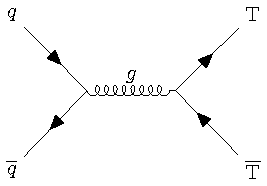
\includegraphics[width=0.6\linewidth]{Images/T_prod_qcd.pdf}
\captionof{figure}{Representative Feynman diagram for T pair production via gluon-mediated QCD processes.\label{fig:qcd_T_prod}}  
\end{center}

\begin{center}
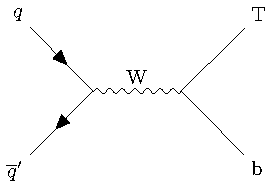
\includegraphics[width=0.6\linewidth]{Images/T_prod_qed.pdf}
\captionof{figure}{Representative Feynman diagram for single T production via electroweak processes.\label{fig:qed_T_prod}}  
\end{center}



In those studies, \textrm{T} decays into $\mathrm{bW}$, $\mathrm{tZ}$, or $\mathrm{tH}$ have been considered. In the context of \textrm{T} pair production, $\mathrm{T}\bar{\mathrm{T}}$, via QCD processes, the cross sections are well-known and solely depend on the mass of the vector-like quark.  Assuming a narrow $\mathrm{T}$ decay width ($\Gamma / m(\mathrm{T}) < 0.05$ or $0.1$) and a $100$\% branching fraction to $\textrm{bW}$, $\textrm{tZ}$, or $\textrm{tH}$, these searches have set stringent bounds on $m(\mathrm{T})$, excluding masses below almost $1.5$ \textrm{TeV} at $95$\% confidence level~\parencite{CMS:2024bni,CMS:2024qdd,ATLAS:2022ozf,ATLAS:2023bfh,ATLAS:2022hnn,ATLAS:2022tla,ATLAS:2023pja,ATLAS:2024fdw}. The most recent analysis from the CMS collaboration probes T-quark production via $\mathrm{pp} \to \mathrm{T}\textrm{qb}$, in final states with $\mathrm{T} \to \textrm{tZ}$ or $\mathrm{T} \to \textrm{tH}$, considering scenarios with preferential couplings to third-generation fermions. The analysis sets $95$\% confidence level upper limits of $68-1260$ \textrm{fb} on the production cross section, for T masses ranging from 600-1200 \textrm{GeV}~\parencite{CMS:2024qdd}. The latest studies from ATLAS probe vector-like quarks using the single-T production mode with the $\mathrm{T} \to \textrm{tH}$ decay channel leading to a fully hadronic final state~\parencite{ATLAS:2022ozf}, the single-\textrm{T} production mode with the $\mathrm{T} \to \textrm{tZ}$ decay channel leading to a multileptonic final state~\parencite{ATLAS:2023bfh}, the \textrm{TT} pair production mode with various \textrm{T} decay channels leading to multileptonic final states~\parencite{ATLAS:2022hnn}, and the \textrm{TT} pair production mode with various \textrm{T} decay channels leading to a single lepton plus missing momentum final state~\parencite{ATLAS:2022tla,ATLAS:2023pja}. 
The multilepton search offers the greatest sensitivity in most of the phase space, but the missing transverse energy based search has better sensitivity for low branching fraction $\mathfrak{B}(\mathrm{T}\to \textrm{Wb})$ and high $\mathfrak{B}(\mathrm{T}\to \textrm{Ht})$. These searches have similar sensitivities for the singlet and doublet models, resulting in exclusion bounds for masses below about $1.25$ \textrm{TeV} and $1.41$ \textrm{TeV}, respectively. 


A key consideration in the model interpretations summarized above is that the $\mathrm{T}$ branching fractions depend on the chosen model. The excluded mass range is less restrictive for specific branching fraction scenarios, such as $\{\mathfrak{B}(\mathrm{T} \to \textrm{tZ})$, $\mathfrak{B}(\mathrm{T} \to bW)$, $\mathfrak{B}(\mathrm{T} \to \textrm{tH})\}= \{0.2, 0.6, 0.2\}$, setting bounds on masses below about $0.95$ \textrm{TeV}. Moreover, if the $\mathrm{T} \to \phi't $ decay is allowed, or if the branching fractions $\mathfrak{B}(\mathrm{T} \to \textrm{tH/bW})$ are lower, the limits previously quoted must be re-evaluated. The authors of Ref.~\parencite{Cacciapaglia:2019zmj} emphasize that bounds on $m(\mathrm{T})$ can be around $500$ \textrm{GeV} when $\mathrm{T} \to \mathrm{t}\phi'$ decays are permitted. Therefore, to facilitate a comprehensive study, benchmark scenarios in this paper are considered down to $m(\chi_\mathrm{u}) = 500$ \textrm{GeV}.

\section{The Minimal $U(1)_{T_R^3}$ Model}\label{sec:model}

% \subsection{Scalar Potential}

The model extends the SM by an Abelian gauge symmetry $U(1)_{T^3_R}$, under which only the right-handed fermions are charged. The symmetry breaking is achieved via two independent Higgs mechanisms: one with the SM Higgs doublet $H$ for electroweak symmetry breaking, and another with a Higgs singlet $\phi$ for breaking $U(1)_{T^3_R}$. These scalars acquire independent vacuum expectation values (VEVs), $\langle H \rangle = v_h / \sqrt{2}$ and $\langle \phi \rangle = v_\phi / \sqrt{2}$. In the Kibble parametrization, the fields are written as:
\begin{align}
    H & = \begin{pmatrix}
        G_{+} \\
        \frac{1}{\sqrt{2}}\left(v_h + \rho_0 + i G_{0}\right)
    \end{pmatrix}, \label{eq:higgskibblepara1} \\
    \phi & = \frac{1}{\sqrt{2}}\left(v_\phi + \rho_\phi + i G_{\phi}\right). \label{eq:higgskibblepara2}
\end{align}
In Eqs.~\eqref{eq:higgskibblepara1} and~\eqref{eq:higgskibblepara2}, $G_\pm$, $G_0$, and $G_\phi$ are the Goldstone bosons absorbed by the SM $W^\pm$ and $Z$ bosons and the dark photon $A'$ (associated with $U(1)_{T^3_R}$) to acquire mass. The fields $\rho_h$ and $\rho_\phi$ mix to form the physical mass eigenstates, the SM-like Higgs boson $h$ and a dark Higgs $\phi'$:
\begin{equation}
    \begin{pmatrix}
        h \\
        \phi'
    \end{pmatrix}
    =
    \begin{pmatrix}
        \cos\alpha & -\sin\alpha \\
        \sin\alpha & \cos\alpha
    \end{pmatrix}
    \begin{pmatrix}
        \rho_0 \\
        \rho_\phi
    \end{pmatrix}.
\end{equation}
This mixing arises from diagonalizing the mass matrix derived from the gauge-invariant scalar potential:
\begin{equation}
    \begin{aligned}
        V(H, \phi) &= \mu_H^2 H^\dagger H + \mu_\phi^2 \phi^* \phi \\
                    &\quad + \lambda (H^\dagger H)(\phi^* \phi) + \lambda_H (H^\dagger H)^2 + \lambda_\phi (\phi^* \phi)^2.
    \end{aligned}
\end{equation}
Minimizing the potential yields the tadpole equations:
\begin{align}
    \frac{\partial V}{\partial H} &= \frac{v_h}{\sqrt{2}} \left( \mu_H^2 + \lambda_H v_h^2 + \frac{1}{2} \lambda v_\phi^2 \right) = 0, \\
    \frac{\partial V}{\partial \phi} &= \frac{v_\phi}{\sqrt{2}} \left( \mu_\phi^2 + \lambda_\phi v_\phi^2 + \frac{1}{2} \lambda v_h^2 \right) = 0.
\end{align}
The physical scalar masses are given by:
\begin{equation}
    m_{h,\phi'}^2 = \frac{1}{2} \left( \lambda_H v_h^2 + \lambda_\phi v_\phi^2 \right) \pm \sqrt{ \lambda^2 v_h^2 v_\phi^2 + \left( \lambda_H v_h^2 - \lambda_\phi v_\phi^2 \right)^2 },
\end{equation}
and the mixing angle $\alpha$ satisfies:
\begin{equation}
    \tan 2\alpha = \frac{-\lambda v_h v_\phi}{ \lambda_\phi v_\phi^2 - \lambda_H v_h^2}.
\end{equation}
The quartic couplings can be expressed in terms of the physical parameters:
\begin{align}
  \lambda_H &= \frac{m_{\phi'}^2 + m_h^2 + (m_{\phi'}^2 - m_h^2)\cos 2\alpha}{4 v_h^2}, \\
  \lambda_\phi &= \frac{m_{\phi'}^2 + m_h^2 + (m_{\phi'}^2 - m_h^2)\cos 2\alpha}{4 v_\phi^2}, \\
  \lambda &= \frac{m_{\phi'}^2 - m_h^2}{2 v_h v_\phi} \sin 2\alpha.
\end{align}
Thus, the scalar sector has four free parameters: the masses $m_h$ and $m_{\phi'}$, the mixing angle $\alpha$, and the dark Higgs VEV $v_\phi$. Similar to how $v_h$ is fixed by the electroweak gauge boson masses, $v_\phi$ is related to the dark photon mass by $m_{A'}^2 = g_{T^3_R}^2 v_\phi^2$, where $g_{T^3_R}$ is the $U(1)_{T^3_R}$ gauge coupling. Depending on the value of $g_{T^3_R}$, this gauge boson can behave as a heavy $Z'$ or a light dark photon. In this chapter, we assume $g_{T^3_R}$ is sufficiently small such that $A'$ can be treated as a dark photon.

\subsection{The Universal Seesaw Mechanism}

In this model, the masses of the SM fermions are generated through a universal seesaw mechanism by mixing with vector-like fermions $\chi_f$. The relevant mass terms in the Lagrangian are:
\begin{equation}
    -\mathcal{L} \supset Y_{f_L} \bar{f}_L' \chi_{fR}' H + Y_{f_R} \bar{\chi}_{fL}' f_R' \phi^* + m_{\chi_f'} \bar{\chi}_{f L}' \chi_{f R}' + \text{h.c.}
\end{equation}
This leads to the mass matrix:
\begin{equation}
    M_f = \begin{pmatrix}
        0 & Y_{f_L} v_h / \sqrt{2} \\
        Y_{f_R} v_\phi / \sqrt{2} & m_{\chi_f'}
    \end{pmatrix}.
\end{equation}
The mass eigenstates $(f, \chi_f)$ are obtained by rotating the gauge eigenstates:
\begin{equation}
    \begin{pmatrix}
        f_{L,R} \\
        \chi_{f_{L,R}}
    \end{pmatrix}
    =
    \begin{pmatrix}
        \pm \cos\theta_{f_{L,R}} & \mp \sin \theta_{f_{L,R}} \\
        \sin \theta_{f_{L,R}} & \cos\theta_{f_{L,R}}
    \end{pmatrix}
    \begin{pmatrix}
        f_{L,R}' \\
        \chi_{f_{L,R}}'
    \end{pmatrix},
\end{equation}
such that $\mathcal{R}(\theta_{f_L}) M_f \mathcal{R}^{-1}(\theta_{f_R}) = \text{diag}(m_f, m_{\chi_f})$. For real parameters, the physical masses and mixing angles are given by:
\begin{gather}
    m_f m_{\chi_f} = \frac{ Y_{f_L} v_h Y_{f_R} v_\phi }{2}, \label{eq:prodmass} \\
    m_f^2 + m_{\chi_f}^2 = m_{\chi_f'}^2 + \frac{1}{2} \left( Y_{f_L}^2 v_h^2 + Y_{f_R}^2 v_\phi^2 \right), \label{eq:summass} \\
    \tan \theta_{f_{L,R}} = \frac{\sqrt{2}}{m_{\chi_f'}} \left( \frac{Y_{f_{L,R}} v_{h,\phi}}{2} - \frac{m_f^2}{Y_{f_{L,R}} v_{h,\phi}} \right).
\end{gather}
The Yukawa interactions of the physical fermions with the scalars $h$ and $\phi'$ are:
\begin{equation}
    -\mathcal{L}_{\text{yuk}} = h \, \bar{\psi}_{f_L} \, \mathcal{Y}_{h} \, \psi_{f_R} + \phi' \, \bar{\psi}_{f_L} \, \mathcal{Y}_{\phi} \, \psi_{f_R},
\end{equation}
where $\psi_f = (f, \chi_f)^T$. The Yukawa matrices are:
\begin{align}
    \mathcal{Y}_{h} &= \frac{1}{\sqrt{2}} \mathcal{R}(\theta_{f_L}) \left( Y_{f_L} \sigma_+ \cos\alpha - Y_{f_R} \sigma_- \sin\alpha \right) \mathcal{R}^{-1}(\theta_{f_R}), \label{eq:YukawaL} \\
    \mathcal{Y}_{\phi} &= \frac{1}{\sqrt{2}} \mathcal{R}(\theta_{f_L}) \left( Y_{f_L} \sigma_+ \sin\alpha + Y_{f_R} \sigma_- \cos\alpha \right) \mathcal{R}^{-1}(\theta_{f_R}), \label{eq:YukawaR}
\end{align}
with $\sigma_{\pm} = (\sigma_1 \pm i \sigma_2)/2$ being the ladder Pauli matrices.

The expressions above provide a simplified, one-generation view. The complete model involves a non-trivial flavor structure where the mass matrices are general $3 \times 3$ matrices. The diagonalization of the full $6 \times 6$ mass matrices, the procedure for absorbing unphysical unitary rotations, and the emergence of the CKM matrix are detailed in Appendix~\ref{app:universal_seesaw}. Furthermore, the appendix contains a rigorous treatment of the mass eigenvalue problem, deriving the exact relationship between the fundamental parameters $(m_L, m_R, m_\chi)$ and the physical observables $(m_f, m_F, \theta_L)$, which leads to critical constraints on the model's parameter space to ensure perturbativity.



\subsection{Minimal UV-complete Theory}

To generate non-zero masses for all SM fermions and ensure gauge anomaly cancellation, the model must include at least one full generation of vector-like fermions $\{\chi_\mathrm{u}, \chi_\mathrm{d}, \chi_\mathrm{\ell}, \chi_\mathrm{\nu}\}$ and the right-handed neutrinos $\nu_R$ for each SM generation. Their quantum numbers are listed in Table~\ref{tab:QMnumbers}. The Yukawa interactions in the UV-complete theory are:
\begin{equation}
    \begin{aligned}
        -\mathcal{L} \supset&\,
        Y_{L u}^{ij} \bar{q}_L^{\prime i} \chi_{u R}^{\prime j} \widetilde{H}
        + Y_{R u}^{ij} \bar{\chi}_{u L}^{\prime i} u_R^{\prime j} \phi^*
        + m_{\chi_\mathrm{u}}^{ij} \bar{\chi}_{u L}^{\prime i} \chi_{u R}^{\prime j} \\
        &+ Y_{L d}^{ij} \bar{q}_L^{\prime i} \chi_{d R}^{\prime j} H
        + Y_{R d}^{ij} \bar{\chi}_{d L}^{\prime i} d_R^{\prime j} \phi
        + m_{\chi_d}^{ij} \bar{\chi}_{d L}^{\prime i} \chi_{d R}^{\prime j} \\
        &+ Y_{L \ell}^{ij} \bar{\ell}_L^{\prime i} \chi_{\ell R}^{\prime j} H
        + Y_{R \ell}^{ij} \bar{\chi}_{\ell L}^{\prime i} \ell_R^{\prime j} \phi
        + m_{\chi_\ell}^{ij} \bar{\chi}_{\ell L}^{\prime i} \chi_{\ell R}^{\prime j} \\
        &+ Y_{L \nu}^{ij} \bar{\ell}_L^{\prime i} \chi_{\nu R}^{\prime j} \widetilde{H}
        + Y_{R \nu}^{ij} \bar{\chi}_{\nu L}^{\prime i} \nu_R^{\prime j} \phi^*
        + m_{\chi_\nu}^{ij} \bar{\chi}_{\nu L}^{\prime i} \chi_{\nu R}^{\prime j}
        + \text{h.c.}
    \end{aligned}
\end{equation}
Here, $i, j = 1,2,3$ are generation indices. The diagonalization of the mass matrices for each fermion type follows the structure outlined in Eqs.~\eqref{eq:prodmass} and~\eqref{eq:summass}, while the Yukawa matrices generalize the structure of Eqs.~\eqref{eq:YukawaL} and~\eqref{eq:YukawaR}, now encoding the CKM and PMNS mixing matrices. The neutrino sector has a more complex structure due to the possibility of a Majorana mass term for the vector-like neutrinos $\chi_\nu'$.

\begin{table}[h!]
    \centering
    \begin{tabular}{ccccc}
        \hline
        \hline
        Field & $SU(3)_C$  & $SU(2)_L$ & $U(1)_Y$ & $U(1)_{T^3_R}$ \\
        \hline\hline
        $q_L'$                    & \textbf{3} & \textbf{2} & 1/6 & 0\\
        $\ell_L'$                 & \textbf{1} & \textbf{2} & -1/2 & 0\\
        $H$                       & \textbf{1} & \textbf{2} & 1/2 & 0\\
        \hline
        $u_R^{\prime c}$          & \textbf{3} & \textbf{1} & -2/3 & -2\\
        $d_R^{\prime c}$          & \textbf{3} & \textbf{1} & 1/3 & 2\\
        $\ell_R^{\prime c}$       & \textbf{1} & \textbf{1} & 1 & 2\\
        $\nu_R^{\prime c}$        & \textbf{1} & \textbf{1} & 0 & -2\\
        $\phi$                    & \textbf{1} & \textbf{1} & 0 & 2\\
        \hline
        $\chi_{u_L}'$             & \textbf{3} & \textbf{1} & 2/3 & 0\\
        $\chi_{u_R}^{\prime c}$   & \textbf{3} & \textbf{1} & -2/3 & 0\\
        $\chi_{d_L}'$             & \textbf{3} & \textbf{1} & -1/3 & 0\\
        $\chi_{d_R}^{\prime c}$   & \textbf{3} & \textbf{1} & 1/3 & 0\\
        $\chi_{\ell_L}'$          & \textbf{1} & \textbf{1} & -1 & 0\\
        $\chi_{\ell_R}^{\prime c}$& \textbf{1} & \textbf{1} & 1 & 0\\
        $\chi_{\nu_L}'$           & \textbf{1} & \textbf{1} & 0 & 0\\
        $\chi_{\nu_R}^{\prime c}$ & \textbf{1} & \textbf{1} & 0 & 0\\
        \hline
        \hline
    \end{tabular}
    \caption{Minimal field content of the model and their representations under the SM and $U(1)_{T^3_R}$ gauge groups.}
    \label{tab:QMnumbers}
\end{table}


\section{Samples and Simulation}\label{sec:sims}


The minimal $U(1)_{T^3_R}$ model described in Sec.~\ref{sec:model} is implemented \textit{at tree level} into the \texttt{FeynRules} package~\parencite{Alloul:2013bka}, which generates the Feynman rules and exports them into a Universal \texttt{FeynRules} Output (\texttt{UFO})~\parencite{Degrande:2011ua}. The resulting \texttt{UFO} is utilized as input for a generator to produce the MC samples. Both signal and background events are generated with the \texttt{MadGraph5\_aMC@NLO} v3.2.0 program~\parencite{Alwall:2014hca,Alwall:2014bza} at leading order (LO) in QCD, considering \textrm{pp} beams colliding with a center-of-mass energy of $\sqrt{s} = 13.6$ \textrm{TeV}. Each signal and background sample is generated separately, with no interference effects between the signal and background considered. The impact of these interference effects has been evaluated, and for all values of $\chi_\mathrm{u}$ and $\phi'$ masses considered, the effect on the signal plus background cross section is found to be less than $<0.5$\%. Additionally, the effect on the shape of the b-jet $p_{T}$ distribution is less than 6\% for $p_{T} < 300$ GeV and less than 2\% for b-jet $p_{T} > 300$ GeV. We use the \texttt{NNPDF3.0~NLO}~\parencite{NNPDF:2014otw} set for parton distribution functions (PDFs) for all event generation. Parton-level events are then interfaced with \texttt{PYTHIA} (v8.2.44)~\parencite{Sjostrand:2014zea} to account for parton showering and hadronization processes. Finally, we use  \texttt{DELPHES} (v3.4.2)~\parencite{deFavereau:2013fsa} to simulate smearing and other detector effects using the CMS detector geometric configurations and parameters for particle identification and reconstruction, using the CMS input card with 140 average pileup interactions.

\begin{center}
  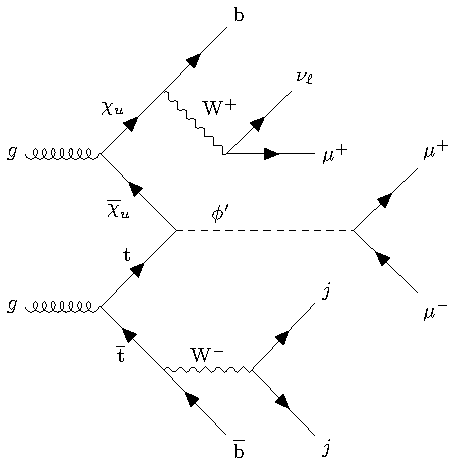
\includegraphics[width=0.75\linewidth]{Images/signal_qqfusion.pdf}
    \captionof{figure}{Representative Feynman diagram for the production of a $\phi'$ boson in association with a $\chi_\mathrm{u}$ vector-like quark through the fusion of a top quark and $\chi_\mathrm{u}$ vector-like quark. Once again, the $\phi'$ decays to a pair of muons, the top quark decays fully hadronically, and the $\chi_\mathrm{u}$ decays semi-leptonically to muons, neutrinos and $b$-jets.\label{fig:qqfusion}}
\end{center}

\begin{center}
    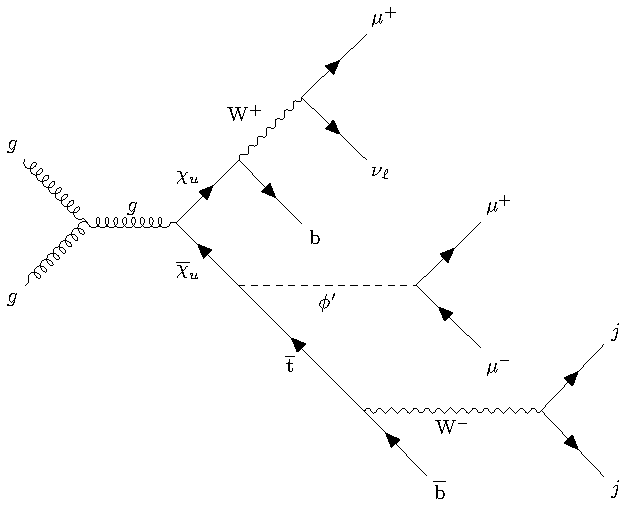
\includegraphics[width=0.85\linewidth]{Images/signal_ggfusion.pdf}
    \captionof{figure}{Representative Feynman diagram for the production of a $\phi'$ boson in association with a $\chi_\mathrm{u}$ vector-like quark through the fusion of a gluon pair from incoming protons. The $\phi'$ decays to a pair of muons, the top quark that decays fully hadronically, and the $\chi_\mathrm{u}$ decay semi-leptonically to muons, neutrinos and jets.\label{fig:ggfusion}}
\end{center}

All signal cross sections used in this analysis are obtained requiring the following kinematic criteria on leptons $\ell$, \textrm{b} quarks, and light-quark/gluon jets ($j$) at parton level in \texttt{MadGraph}: $p_{\mathrm{T}}(\ell) > 35$~\textrm{GeV}, $\abs{\eta (\mathrm{b})} < 2.5$, $\abs{\eta (\ell)} < 2.3$, $p_{\mathrm{T}}(j) > 20$~\textrm{GeV}, and $\abs{\eta (\mathrm{j})} < 5$. These parton-level selections were applied exclusively to the signal processes to restrict event generation to the relevant phase space regions. For background processes, these default parton level requirements in \texttt{MadGraph} were imposed:  $p_{\mathrm{T}}(\ell) > 10$~\textrm{GeV}, $\abs{\eta (\ell)} < 2.5$, $p_{\mathrm{T}}(j) > 20$~\textrm{GeV}, $\abs{\eta (\mathrm{j})} < 5$, and $\abs{\eta (\mathrm{b})} < 5$. This ensures that the phase space regions for the background near the analysis-level selection criteria are adequately described after parton showering since the pre-selections at the analysis level are more stringent than the parton-level requirements. Furthermore, we use the MLM algorithm for jet matching and jet merging. The parameters \texttt{xqcut} and \texttt{qcut} of the MLM algorithm are set to 30 and 45 respectively to ensure continuity of the differential jet rate as a function of jet multiplicity. Each simulated signal and background sample is produced separately at LO, with one million events at the generation level, neglecting potential interference effects between the signal and background due to the suppression caused by the different orders of magnitude in the coupling constants of the signal and background.

Signal samples are generated considering the production of a $\phi'$ boson, an associated $\chi_\mathrm{u}$ vector-like quark, and a top quark $(\mathrm{pp}\to \chi_\mathrm{u} \mathrm{t} \phi')$, inclusive in both $\alpha$ and $\alpha_s$ (see Figures~\ref{fig:qqfusion}-\ref{fig:ggfusion}). We have used the implementation of the $U(1)_{T^3_R}$ model in Ref.~\parencite{Dutta2023}. Signal samples were created considering coupling values of $Y_{\mathrm{t}_R}=Y_{\mathrm{t}_L}=2\sqrt{2}$ in the range of masses $m(\phi')\in\{5,10,50,100,325\}$~\textrm{GeV} for the dark higgs and $m(\chi_\mathrm{u})\in\{0.50, 0.75, 1.0, 1.5, 2.0, $ $ 2.5\}$~\textrm{TeV} for the vector-like quark $\chi_u$~\parencite{PhysRevD.108.095006}. The production cross section for $\mathrm{pp}\to \chi_\mathrm{u} \mathrm{t} \phi'$ is highly dependent on the choice of the Yukawa couplings in the Lagrangian. The ${\chi_\mathrm{u}}{- \mathrm{t}}$ fusion process shown in Fig.~\ref{fig:qqfusion} is dominated by the $Y_{\mathrm{t}_R}$ coupling. However, the decay ${\chi_\mathrm{u}} \to \mathrm{t} \phi'$ shown in Fig.~\ref{fig:ggfusion} is inversely proportional to the $Y_{\mathrm{t}_L}$ coupling. This effect is shown in Fig.~\ref{fig:cross_section_by_lambdas}, which displays the total signal cross section, as a function of $Y_{\mathrm{t}_R}$ and $Y_{\mathrm{t}_L}$, for a benchmark point with $m(\phi')=100$~\textrm{GeV} and $m(\chi_\mathrm{u})=1.0$~\textrm{TeV}. 

\begin{figure}
    \centering
    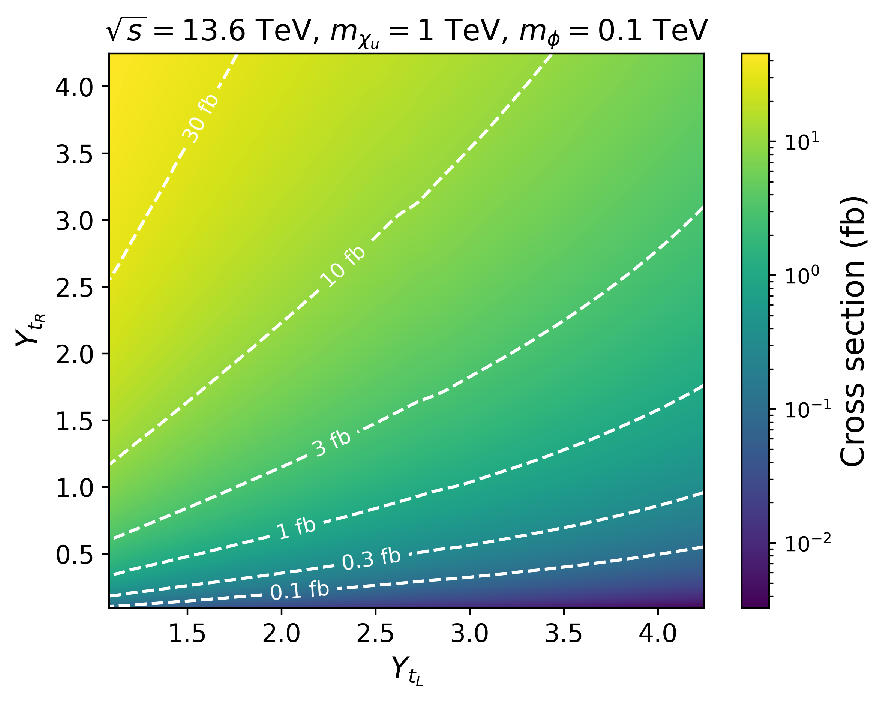
\includegraphics[width=0.85\linewidth]{Images/cross_section_by_lambdas.pdf}
    \caption{Signal production cross section, $ \mathrm{pp}\to \chi_\mathrm{u} \mathrm{t} \phi'$,  in the $Y_{\mathrm{t}_R}$ versus $Y_{\mathrm{t}_L}$ plane, for a benchmark point with $m(\phi')=100$~\textrm{GeV} and $m(\chi_\mathrm{u})=1.00$~\textrm{TeV}. The white-dashed contours show specific cross section values in the two dimensional plane.}
    \label{fig:cross_section_by_lambdas}
\end{figure}

We target signal events where the top quark decays hadronically into a bottom quark and two jets ($\mathrm{t} \to \mathrm{bW} \to \mathrm{b} q \bar{q}'$), the $\chi_\mathrm{u}$ decays semileptonically into a $b$ quark, lepton, and neutrino (via $\chi_\mathrm{u} \to \mathrm{bW}$ and $\mathrm{W}\to\mu\nu_{\mu}$), and the $\phi'$ produces two muons. We note that the scalar $\phi'$ particle could result from the mixture of the SM Higgs boson and additional scalar fields, and the Yukawas of the fermions could additionally arise from the mixing of the SM fermions with additional copies of the associated vector-like fermions. Therefore, the $\phi'$ branching ratios are dependent on the chosen mechanism and model by which this mixture occurs, see for example, Refs.~\parencite{Cacciapaglia_2023,Blankenburg:2012nx,Jones-Perez:2013oia,Calibbi:2009pv}. For the purpose of this work, and 
similar to Refs.~\parencite{Dutta2020,Dutta2023}, the considered benchmark signal scenarios have $\mathfrak{B}(\chi_\mathrm{u} \rightarrow \textrm{b W})$ of about 0.5 and $\mathfrak{B}(\phi' \rightarrow \mu^+\mu^-)=1.00$. Fig.~\ref{fig:xs-plot} shows the production cross section in \textrm{fb}, as a function of $m(\phi')$ and $m(\chi_\mathrm{u})$ masses, assuming the aforementioned decays, branching ratios, and couplings.

We note that for the parameter space of focus in this paper, the total mass of the $t$-$\chi_\mathrm{u}$ system is larger than $m(\phi')$, thus the large rest energy of the $t$-$\chi_\mathrm{u}$ system is converted into potentially large momentum values for the $\phi'$. Similarly, the $t$-quark produced through the $\chi_\mathrm{u}$-$t$ fusion interaction can also have large momentum values, and thus in some cases the hadronic $t$ decay products cannot be fully reconstructed independently of each other. This results in three possible $t$ reconstruction scenarios: a fully merged scenario where the $\mathrm{W}\to jj$ system and the $\mathrm{b}$ quarks are very collimated and reconstructed as a single ``fat jet’’ (henceforth referred to as a FatJet, FJ); a partially merged scenario, where the decay products of the $\mathrm{W}$ boson form a single FatJet but the $\mathrm{b}$ quark can still be separately identified; and an un-merged scenario where all decay products can be independently identified. Jets are clustered using the anti-$k_t$ algorithm~\parencite{Cacciari_2008} using the \texttt{FastJet} (v3.4.2)~\parencite{Cacciari_2012} package with a distance parameter of $R = 0.4$ for standard jets and $R = 0.8$ for fat jet objects. Each scenario has an associated identification efficiency and misidentification rate, which depends on the choice of the boosted $t$/$W$ algorithm (our choice of efficiency and misidentification rates is described later). 

Based on the above details, the final state of interest in this paper consists of three muons (two from the $\phi'$ decay and one from the $\chi_\mathrm{u}$ decay), a (possibly boosted) top-tagged system, at least one $b$-tagged jet, and large missing transverse momentum ($\vec{p}_{T}^{\textrm{~miss}}$). For the partially merged and un-merged scenarios, there will be two $b$ quarks present in the final state (one of which is part of the top tagged system). 

We consider background sources from SM processes which can give similar objects in the final state as those expected for signal. Several background sources were considered and studied, such as QCD multijet events, production of vector boson pairs ($\mathrm{VV: WW, ZZ, WZ}$), vector boson triplets ($\mathrm{VVV: WWZ, WZZ, ZZZ, WWW}$), top-quark pairs in association with weak bosons ($\mathrm{t}\overline{\mathrm{t}}X$), and $\mathrm{t}\overline{\mathrm{t}}\mathrm{t}\overline{\mathrm{t}}$ processes. The  dominant sources of SM background events are from the $\mathrm{t}\overline{\mathrm{t}}X$, $\mathrm{ZZW}$, and $\mathrm{t}\overline{\mathrm{t}}\mathrm{t}\overline{\mathrm{t}}$ processes. The $\mathrm{t}\overline{\mathrm{t}}X$ background is primarily associated production of a $\mathrm{Z}/\gamma^{*}$ from $\mathrm{t}\bar{\mathrm{t}}$ fusion processes. The $\mathrm{ZZW}$ process becomes a background when one $\mathrm{Z}$ decays $\mathrm{b}\bar{\mathrm{b}}$, another $\mathrm{Z}$ decays to a pair of muons, and the W decays to a muon and a neutrino. 
Events from $\mathrm{ZZW}$ and $\mathrm{t}\overline{\mathrm{t}}\mathrm{t}\overline{\mathrm{t}}$ have been combined, after being weighted by their corresponding production cross section. The combination is presented as the ``$\mathrm{b} \overline{\mathrm{b}}\mu\mu\mu\nu$'' background in the remainder of this paper. The $\mathrm{t}\overline{\mathrm{t}}X$ process is presented as part of the ``$\mathrm{t}\overline{\mathrm{t}}\mu^{+}\mu^{-}$'' background. Tab.~\ref{tab:dominantbkgs} shows the production cross sections for the dominant background sources. The rest of the aforementioned background processes do not contribute meaningfully in our context, accounting for $\ll 1\%$ of the total expected background yield.

The identification of leptons, boosted top quarks, and bottom quarks plays an important role in the ability to identify signal events, the ability to minimize the rate of SM backgrounds, and thus also the discovery reach in the high-luminosity environment of the LHC. It is worth noting that the reconstruction and identification of leptons and the decay products of the top/bottom quarks may be non-trivial at the High-Luminosity LHC (HL-LHC) due to the presence of a potentially large number of secondary pp interactions (pileup). The impact of pileup on the new physics discovery reach, and the importance of pileup mitigation at CMS and ATLAS has been outlined in many papers, for example in Ref.~\parencite{CMS-PAS-FTR-13-014}. We note the expected performance of the upgraded ATLAS and CMS detectors for the HL-LHC is beyond the scope of this work; however, the studies presented here do attempt to provide reasonable expectations by conservatively assuming some degradation in lepton and hadron identification efficiencies, using Ref.~\parencite{CMS-PAS-FTR-13-014} as a benchmark, and considering the case of 140 average pileup interactions. 

For muons with $|\eta|< 1.5$, the assumed identification efficiency is 95\% with a 0.3\% misidentification rate~\parencite{CMS-PAS-FTR-13-014,CMS_MUON_17001}. The performance degrades linearly with $\eta$ for $1.5 < |\eta| < 2.5$, and we assume an identification efficiency of 65\% with a 0.5\% misidentification rate at $|\eta| = 2.5$. Similarly, the charged hadron tracking efficiency, which contributes to the jet clustering algorithm and missing transverse momentum ($\vec{p}_{T}^{\textrm{~miss}}$) calculation, is 97\% for $1.5 < |\eta| < 2.5$, and degrades to about 85\% at $|\eta| = 2.5$. These potential inefficiencies due to the presence of secondary pp interactions contribute to how well the lepton and top kinematics can be reconstructed. Following Refs.~\parencite{CMS:2020poo,ATLAS:2018wis}, we consider the ``Loose'' working point for the identification of the fully merged (partially merged) $\mathrm{t}$ decays, which results in 80-85\% top (W) identification efficiency and 11-25\% misidentification rate, depending on the FatJet transverse momentum ($p_{T}^{FJ}$). Following Ref.~\parencite{CMSbtag}, we consider the ``Loose'' working point of the DeepCSV algorithm~\parencite{Bols_2020}, which gives a 70-80\% b-tagging efficiency and 10\% light quark mis-identification rate. The choice of boosted $t$/$W$ and b-tagging working points is determined through an optimization process that maximizes discovery reach. It is noted the contribution from SM backgrounds with a misidentified boosted $t$/$W$ is negligible, and thus our discovery projections are not sensitive to uncertainties related to the boosted $t$/$W$ misidentification rates. 

\begin{figure}
    \centering
    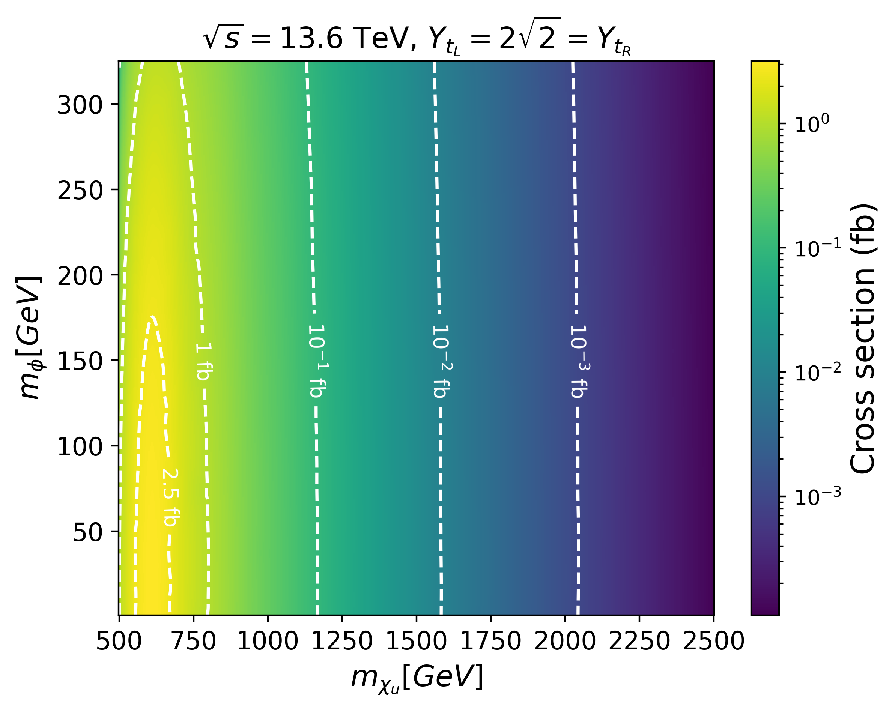
\includegraphics[width=0.85\linewidth]{Images/cross_section_by_masses.pdf}
    \caption{Projected cross section (fb) plot for $pp\to t \chi_\mathrm{u} \phi'$ and subsequent decay as a function of $m(\chi_\mathrm{u})$ and $m(\phi')$.}
    \label{fig:xs-plot}
\end{figure}

\begin{table}[]
  \begin{tabular}{l r}
    \hline
    {Background Process} & {Cross-Section $\sigma$ [\textrm{pb}]} \\
    \hline
   $\mathrm{pp} \to \mathrm{t} \overline{\mathrm{t}} \, \mu^+ \mu^-$ & $2.574\times 10^{-3}$  \\
    $\mathrm{pp} \to \mathrm{b}\overline{\mathrm{b}}\, \mu\mu\mu\nu $ & $4.692 \times 10^{-4}$ \\
    \hline
  \end{tabular}
  \centering
  \caption{A summary of dominant SM backgrounds produced by $\mathrm{pp}$ collisions and their cross sections in pb, as computed by \texttt{MadGraph} with $n = 10^6$ events.}
  \label{tab:dominantbkgs}
\end{table}

\begin{figure}[]
\centering
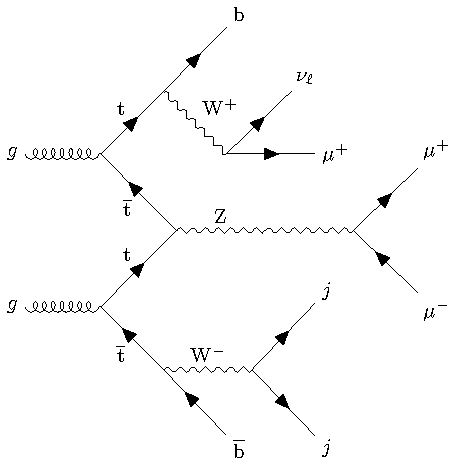
\includegraphics[width=.75\linewidth]{Images/bg_Z_full.pdf}
\caption{Representative Feynman diagram for a background event. A $Z$ boson is produced in association with a top quark through the fusion of a top, anti top pair from incoming protons. The $Z$ boson subsequently decays to a pair of muons and the two spectator top quarks decay semi-leptonically and purely hadronically to muons, neutrinos and jets, resulting in the same final states as the signal event.\label{fig:v}}
\end{figure}


\section{Data Analysis Using Machine Learning}\label{sec:ML}
The analysis of signal and background events is performed utilizing machine learning techniques. A machine learning-based approach offers sizeable advantages when compared to traditional event classification techniques. Unlike conventional methods, machine learning models have the capability to simultaneously consider all kinematic variables, allowing them to efficiently navigate the complex and high-dimensional space of event kinematics. Consequently, machine learning models can effectively enact sophisticated selection criteria that take into account the entirety of this high-dimensional space. This makes them ideal for high-energy physics applications.

The BDT method is a powerful machine learning technique that has proven its effectiveness in various applications, particularly in the field of collider physics. In this method, decision trees are trained greedily in a sequential manner, with each tree focusing on learning the discrepancies or residuals between its predictions and the expected values obtained from the previously trained tree. This iterative process aims to progressively minimize errors, making BDTs a particularly effective approach for enhancing model performance.

In the context of collider physics, BDTs have demonstrated their utility in addressing classification problems. In particular, BDTs can effectively discriminate between signal and background events, enabling accurate and efficient event classification. Their ability to handle subtle non-linear relationships within the data with high interpretability makes BDTs a valuable tool to handle large amounts of data with a large number of parameters for each event. 

The first step in our workflow involves the use of a specialized \texttt{MadAnalysis Expert Mode} C++ script~\parencite{CONTE2013222}. This script extracts essential kinematic and topological information from the simulated samples. The script will process the aforementioned variables contained within these files and transform them into a structured and informative CSV (Comma-Separated Values) format that can be used to train our machine learning models. These kinematic variables include crucial details about the events, such as particle momenta, energies, and topologies, providing the fundamental building blocks for our machine learning analysis. 

To account for the differential significance of various events, we apply cross-section weighting. This ensures that the relative importance of signal and background events is appropriately balanced in the dataset. This weighting is crucial for addressing the varying likelihood of observing different types of events in high-energy physics experiments. The prepared and weighted datasets are then passed to our \texttt{MadAnalysis Expert Mode} C++ script, where the simulated signal and background events are initially filtered, before being passed to the CSV file for use by the machine learning algorithm. The filtering process requires at least one well-reconstructed and identified $\mathrm{b}$-jet candidate, at least one jet (regular or FJ) not tagged as a $\mathrm{b}$ jet, and exactly three identified muons. The filtering selections are motivated by experimental constraints, such as the geometric constraints of the CMS/ATLAS detectors, the typical kinematic thresholds for the reconstruction of particle objects, and the available lepton triggers which also drive the minimal kinematic thresholds. Selected jets must have $p_{\mathrm{T}} > 30$ $\textrm{GeV}$ and $|\eta(j)| < 5.0$, while $\mathrm{b}$-jet candidates with $p_{\mathrm{T}} > 20$ $\textrm{GeV}$ and $|\eta(\mathrm{b})| < 2.5$ are chosen. The $\mu$ object must pass a $p_{\mathrm{T}} > 35$ $\textrm{GeV}$ threshold and be within a $|\eta(\ell)| < 2.3$. We will refer to this filtering criteria as pre-selections. The efficiency of the pre-selections depends on $m(\phi')$ and $m(\chi_{\mathrm{u}})$, but is typically about $25-30$\% for the signal samples. Events passing this pre-selection are used as input for the machine learning algorithm, which classifies them as signal or background, using a probability factor. 



We explore the performance of a diverse set of machine learning models, specifically three neural networks of differing architectures and a BDT algorithm. To ensure robust model assessment, we employed a standard 90-10 train-test split of the dataset, partitioning it into a 90\% portion for training and a 10\% portion for testing. This division allows us to gauge the generalization capabilities of our models on unseen data.  

The training and evaluation of the BDT were carried out in a high-performance computing environment. Specifically, an Nvidia A100 GPU was used. The canonical \texttt{PyTorch}~\parencite{paszke2019} deep learning framework was employed for configuring, training, and evaluating the neural networks. PyTorch is well-regarded for its flexibility and performance in deep learning applications.

For the BDT algorithm, we used hyperparameters $\eta=0.3$, $\gamma = 0$, and $\texttt{max\_depth} = 6$. The \texttt{XGBoost}~\parencite{chen_xgboost_2016} library was used for the implementation of the Boosted Decision Tree algorithm. It offers high efficiency, optimization, and interpretability, making it a suitable choice for this particular task. 



\begin{table}
    \centering
    \begin{tabular}{c  c  c}
    \hline
    { Model} & { Train/Test Acc. } & { Training Time} \\
    \hline
    \small
    BDT & N.A./0.9993  & 6s\\
    Neural Network 1 & 0.9999/0.9997 & 1h 58m \\
    Neural Network 2 & 0.9999/0.9998 & 2h 12m \\
    Neural Network 3 & 0.9999/0.9998 & 2h 32m\\
    \hline
    \end{tabular}
    \caption{Train/test results for the ML models.}\label{tab:ml_results}
    \centering
\end{table}

It is worth mentioning that we experimented with deep neural networks of various architectures. Although we found that they yield similar signal sensitivity to the BDT, the complex nature of the studies in this
work (particle objects considered, experimental constraints in a high luminosity LHC, etc.) motivates the use of a BDT over a deep neural network because of its usefulness, efficiency, and simplicity in understanding the machine learning output in addition to significantly shorter training times. Therefore, we perform our proceeding analysis using the BDT. The outcomes of our model training and evaluation are presented in Table 3. 

\section{Results}\label{sec:results}
Figures~\ref{fig:_mu12},~\ref{fig:pTb1}, and~\ref{fig:pTmu1} show relevant kinematic distributions for two benchmark signal points and the dominant SM backgrounds, using the subset of events passing the pre-selections defined above. The signal benchmark points in these figures are $m(\phi^{'}) = 325 \, \mathrm{GeV}$, $m(\chi_{\mathrm{u}}) = 2\, \mathrm{TeV}$, and $m(\phi^{'}) = 1 \, \mathrm{GeV}$, $m(\chi_{\mathrm{u}}) = 500\, \mathrm{GeV}$. The distributions are normalized such that the area under the curve is unity. These distributions correspond to the reconstructed mass, $m(\mu_{1}, \mu_{2})$, between the two muon candidates with the highest transverse momentum ($\mu_{1}$ and $\mu_{2}$), 
the transverse momentum of the \textrm{b}-jet candidate with the highest transverse momentum $p_{\mathrm{T}}$ ($\mathrm{b_{1}}$), and the muon candidate with the highest transverse momentum $p_{\mathrm{T}}$ ($\mu_{1}$), respectively. 
Note that the signal distributions exhibit tails that are significantly the backgrounds. These distributions are among the variables identified by the BDT algorithm with the highest signal to background discrimination power.


\begin{figure}
\centering
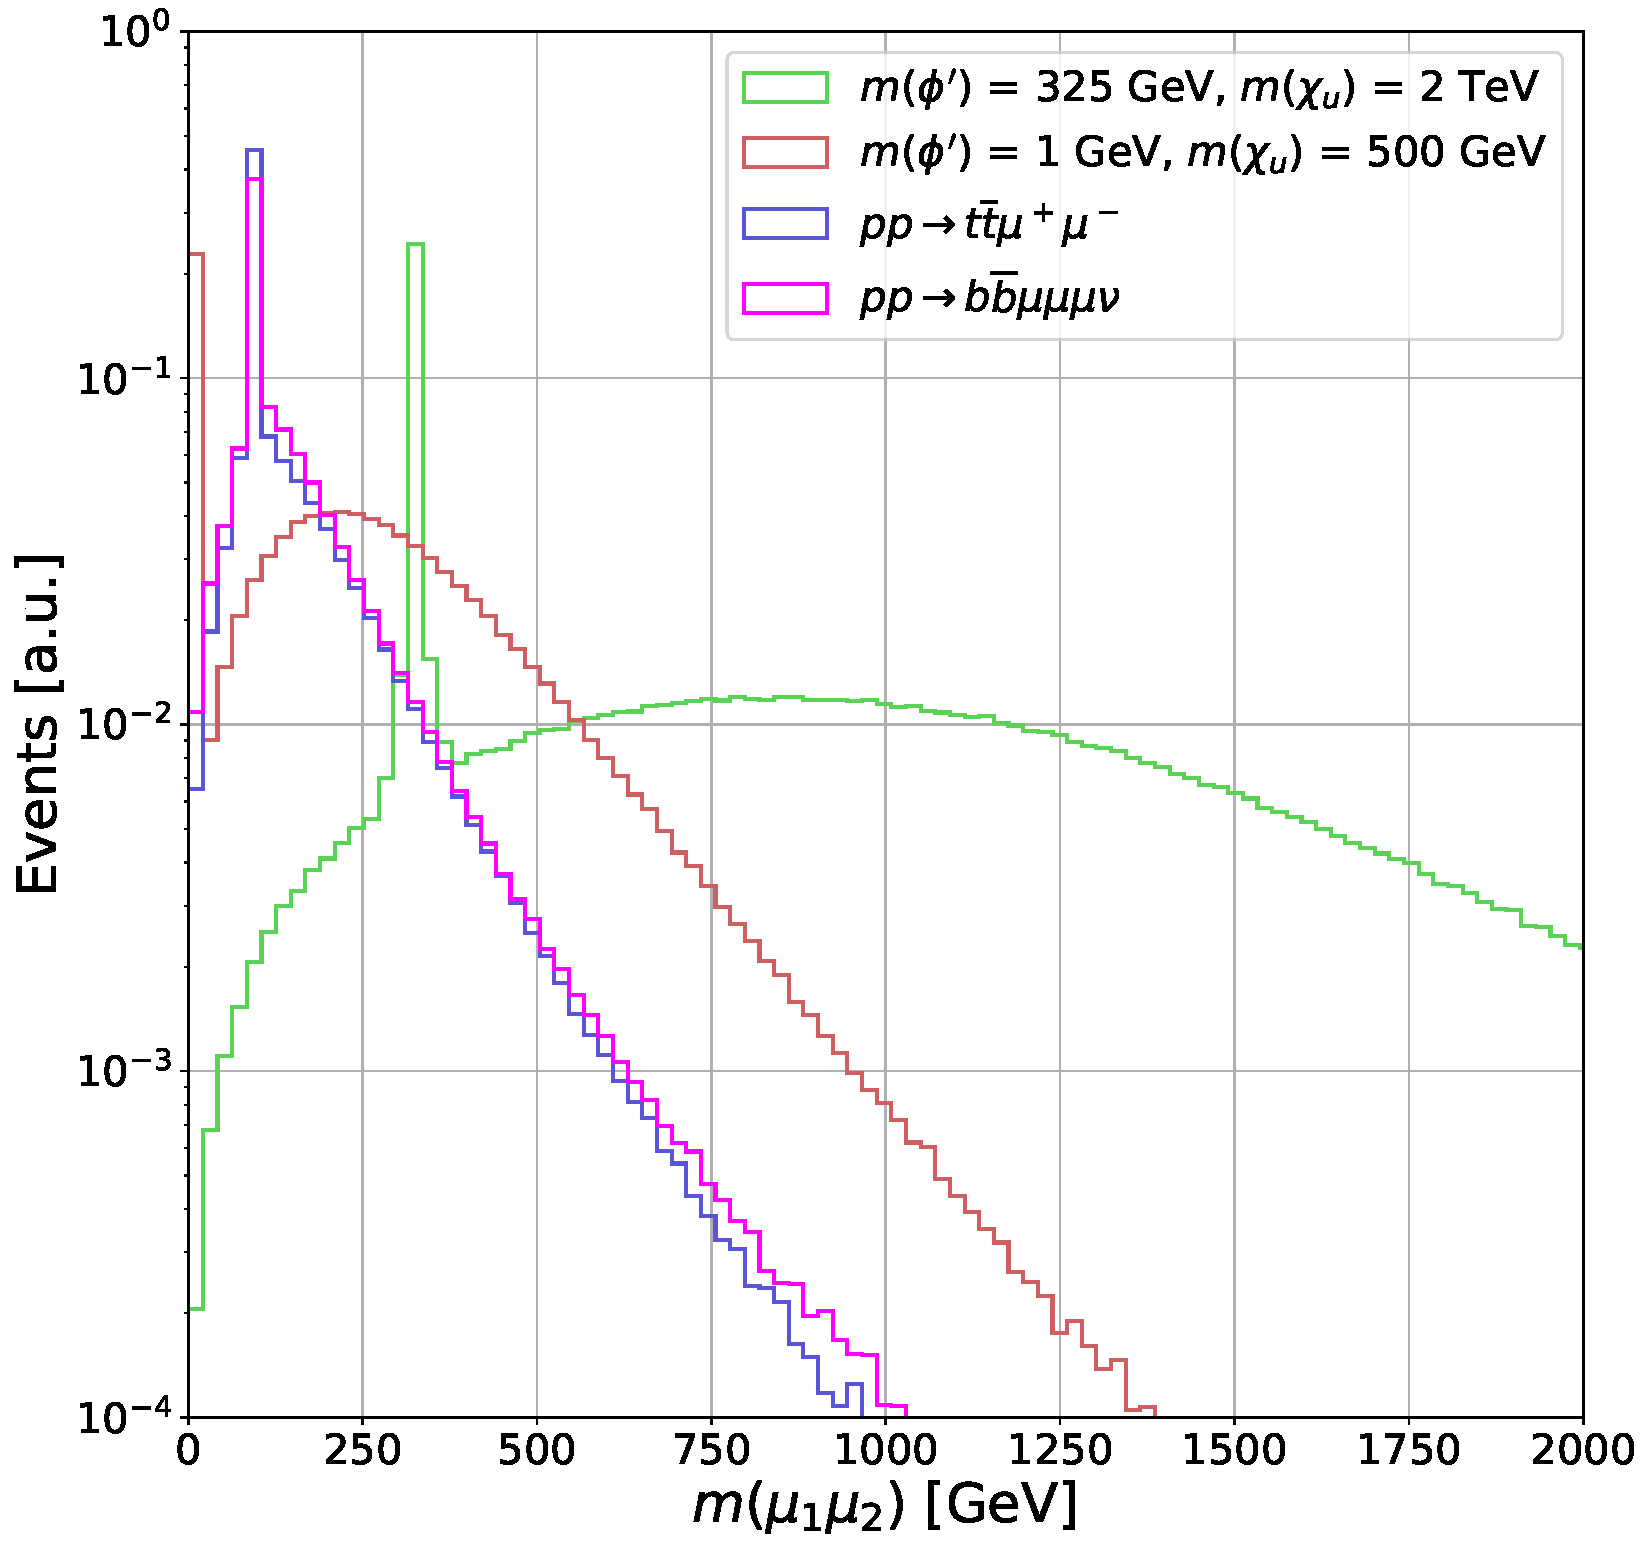
\includegraphics[width=.75\linewidth]{Images/M_mu_1_2.pdf}
\caption{Invariant mass distribution of the muon pair with the highest and second highest transverse momentum. The distributions are shown for the two main SM background processes and two signal benchmark points.\label{fig:_mu12}}
\end{figure}

\begin{figure}
\centering
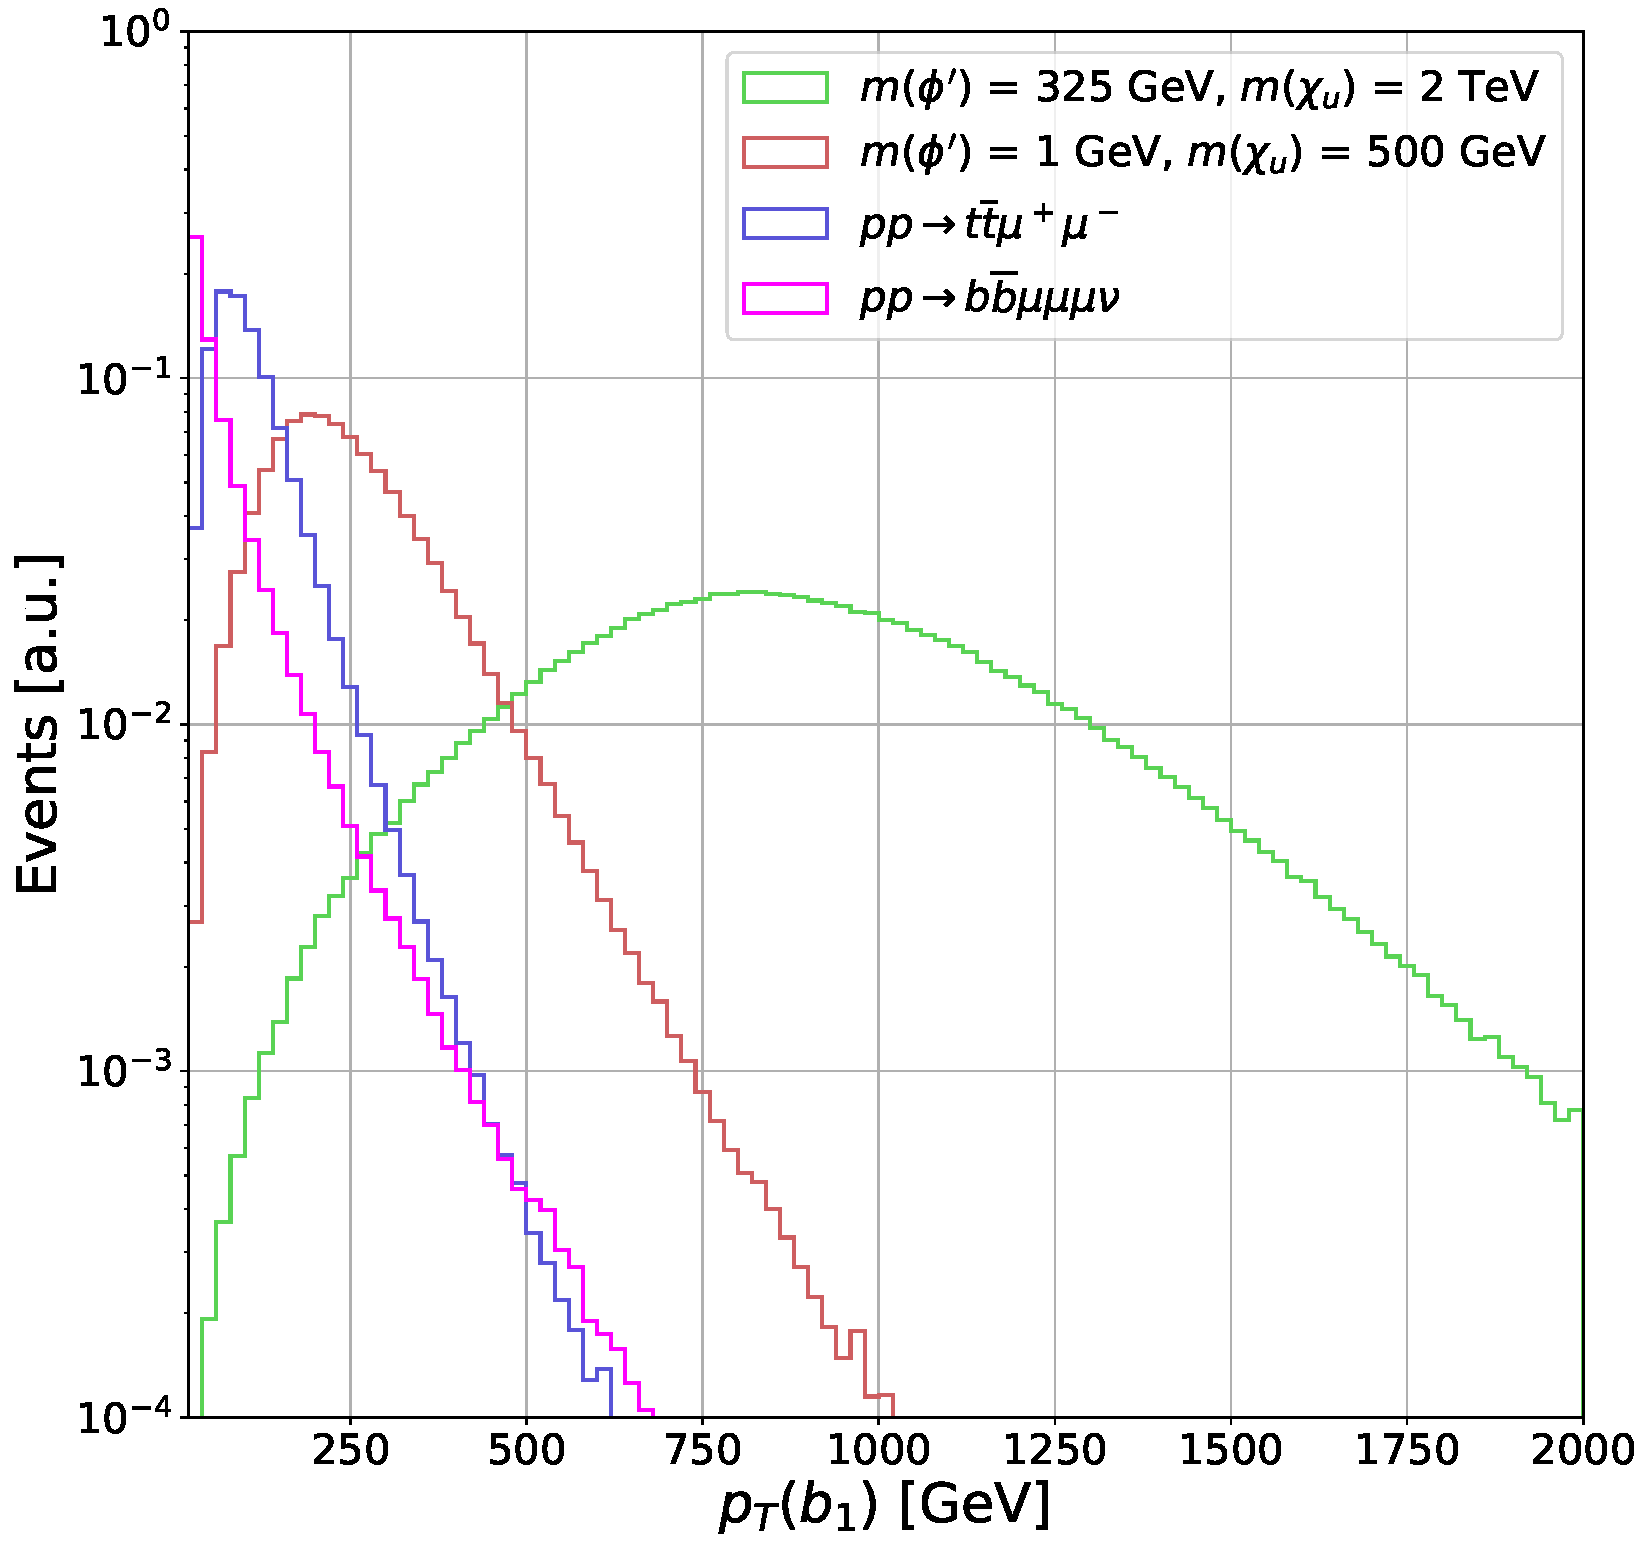
\includegraphics[width=.75\linewidth]{Images/PT_b1.pdf}
\caption{Transverse momentum distribution of the leading \textrm{b}-quark jet candidate. The distributions are shown for the two main SM background processes and two signal benchmark points.\label{fig:pTb1}}
\end{figure}

\begin{figure}
\centering
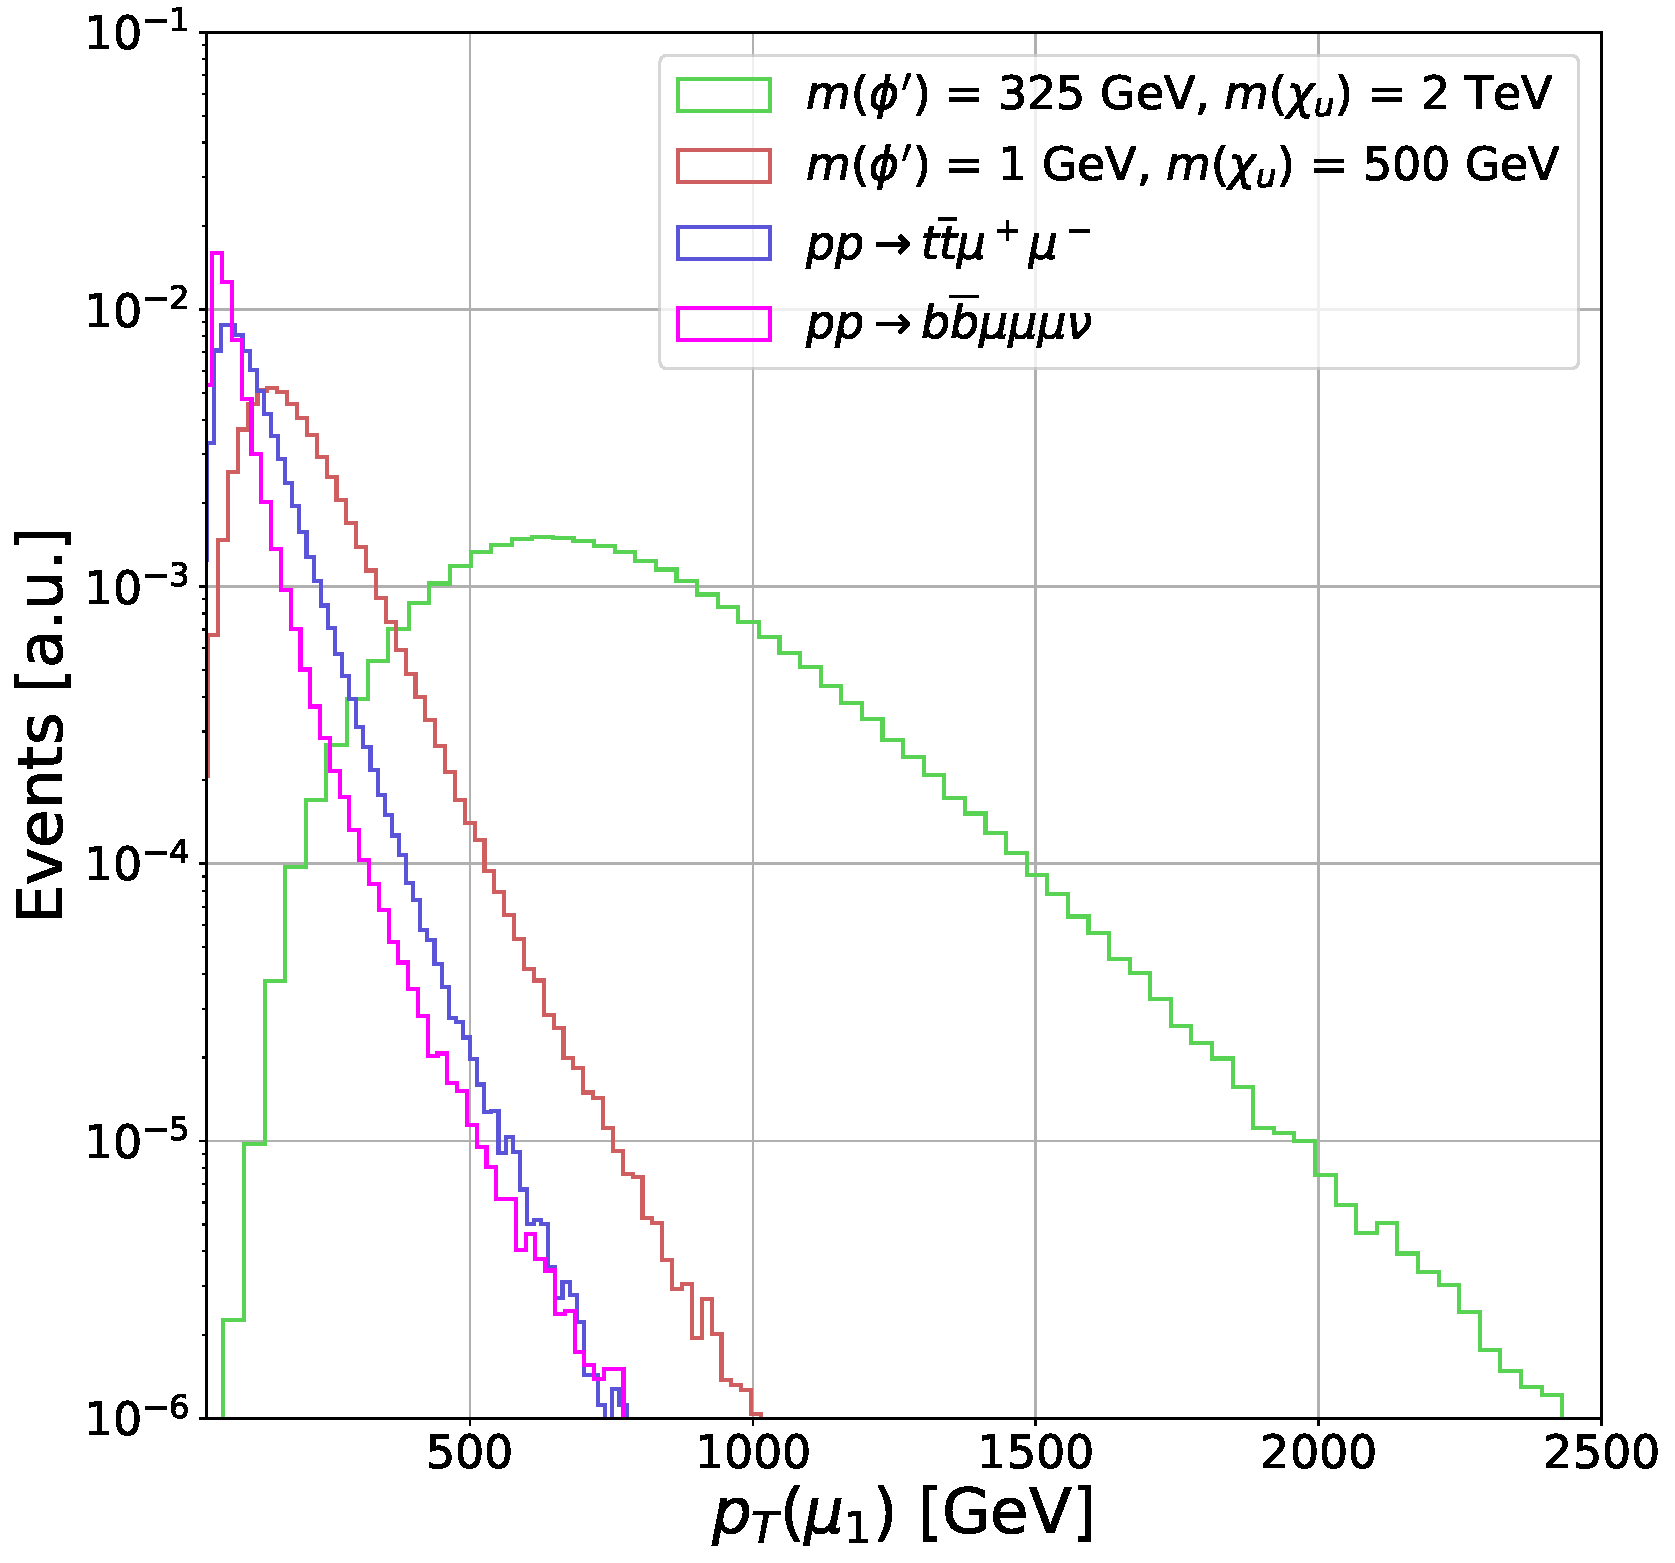
\includegraphics[width=.75\linewidth]{Images/PT_mu1_1.pdf}
\caption{Transverse momentum distribution of the leading muon candidate. The distributions are shown for the two main SM background processes and two signal benchmark points.\label{fig:pTmu1}}
\end{figure}


As can be seen from Fig.~\ref{fig:_mu12}, the $\phi'$ mass can be reconstructed through its associated muon decay pair, which is observed as a peak in the $m(\mu_{1}, \mu_{2})$ distribution around the expected $m(\phi')$ value, and has low- and high-mass tails which are a consequence of cases where the leading and/or subleading muon is not from the $\phi'$ decay, but rather from the associated $\mathrm{W}$ boson from the $\chi_{\mathrm{u}}$ decay. For the backgrounds, muons come from \textrm{Z} (\textrm{W}) decays. Therefore, the $m(\mu_{1}, \mu_{2})$ background distributions show a peak near $m_{\mathrm{W/Z}}$, combined with a broad distribution indicative of the combination of two muon candidates from different decay vertices. We note that the $\phi'\to\mu^{+}\mu^{-}$ decay width depends on the square of the $\phi'\to\mu^{+}\mu^{-}$ coupling and  $\frac{m_{\mu}^{2}}{m_{\phi'}^{2}}$ and is thus suppressed by the relatively small muon mass. For the new physics phase space considered in this paper, the $\phi'$ decay width is less than 1\% of the $\phi'$ resonant mass. Furthermore, as indicated previously, the signal/background interference effects are small and negligible compared to effects from experimental resolution. Therefore, the width of the $m(\mu_{1}, \mu_{2})$ signal distributions is driven by the experimental resolution in the reconstruction of the muon momenta, as well as the probability that the two leading muons are the correct pair from the $\phi'$ decay. Since the probability that the two highest-$p_{\mathrm{T}}$ muons are the correct pair from the $\phi'\to\mu^{+}\mu^{-}$ decay depends on $m(\phi')$ and $m(\chi_\mathrm{u})$, it is important to include all possible combinations of dimuon pairs (i.e., $m(\mu_{1}, \mu_{3})$ and $m(\mu_{2}, \mu_{3})$) in the training of the BDT. 

Fig.~\ref{fig:pTb1} shows the  distribution for the \textrm{b}-jet candidate with the highest $p_{\mathrm{T}}$, $p_{\mathrm{T}}(\mathrm{b}_1)$, for the same simulated samples shown in Fig.~\ref{fig:_mu12}. Based on the signal topology and our choice of parameter space (i.e., $m_{\chi_\mathrm{u}} > m_{\mathrm{t}}$), it is expected that the leading $\mathrm{b}$-jet candidate comes from the $\chi_\mathrm{u}$ decay, with an average $p_{\mathrm{T}}$ close to $\frac{m_{\chi_\mathrm{u}} - m_{\mathrm{W}}}{2}$, as observed in Fig.~\ref{fig:pTb1}. For the $\mathrm{t} \overline{\mathrm{t}} \mu^{+}\mu^{-}$ background, the \textrm{b}-jet candidates come from top-quark decays. Therefore, their average transverse momentum is expected to be $\frac{m_{\mathrm{t}} - m_{\mathrm{W}}}{2} \approx 45$~\textrm{GeV}, as observed in Fig.~\ref{fig:pTb1}. On the other hand, the \textrm{b}-jet candidates for the $\mathrm{b} \overline{\mathrm{b}}\mu\mu\mu\nu$ background can come from off-mass-shell $\mathrm{Z}^{*}/\gamma^{*}$, and thus typically have an even softer spectrum in comparison to the $\mathrm{t} \overline{\mathrm{t}} \mu^{+}\mu^{-}$ background.

Fig.~\ref{fig:pTmu1} shows the  distribution for the muon candidate with the highest $p_{\mathrm{T}}$, $p_{\mathrm{T}}(\mu_{1})$. Similar to Fig.~\ref{fig:pTb1}, when $m(\chi_\mathrm{u}) > m_{\mathrm{t}}$ it is expected that the leading muon candidate comes from the $\chi_\mathrm{u}$ decay, with an average $p_{\mathrm{T}}$ of approximately $\frac{m(\chi_\mathrm{u}) - m_{\mathrm{W}}}{4}$, as observed in Fig.~\ref{fig:pTmu1}. For the major SM backgrounds, the muon candidates come from Z/W/$\gamma^{*}$ decays. Therefore, their average transverse momentum is expected to be much lower, $\frac{m_{\mathrm{Z/W}}}{4} \approx 40-45$~\textrm{GeV}. This kinematic feature provides a nice handle to discriminate high $m(\chi_\mathrm{u})$ signal events amongst the large SM backgrounds, which have lower average $p_{\textrm{T}}(\mu)$ constrained by the SM weak boson masses.

In addition to these aforementioned variables in Figures~\ref{fig:_mu12}-\ref{fig:pTmu1}, several other kinematic variables were included as inputs to the BDT algorithm. In particular, 27 such variables were used in total, and these included the momenta of $\mathrm{b}$ and muon candidates; invariant masses of pairs of muons; angular differences between $\mathrm{b}$ jets and between the muons. Fig.~\ref{fig:feature_importance} shows the features that are used for training the machine learning models and their importance for a benchmark point.

\begin{figure}
\centering
  \centering
  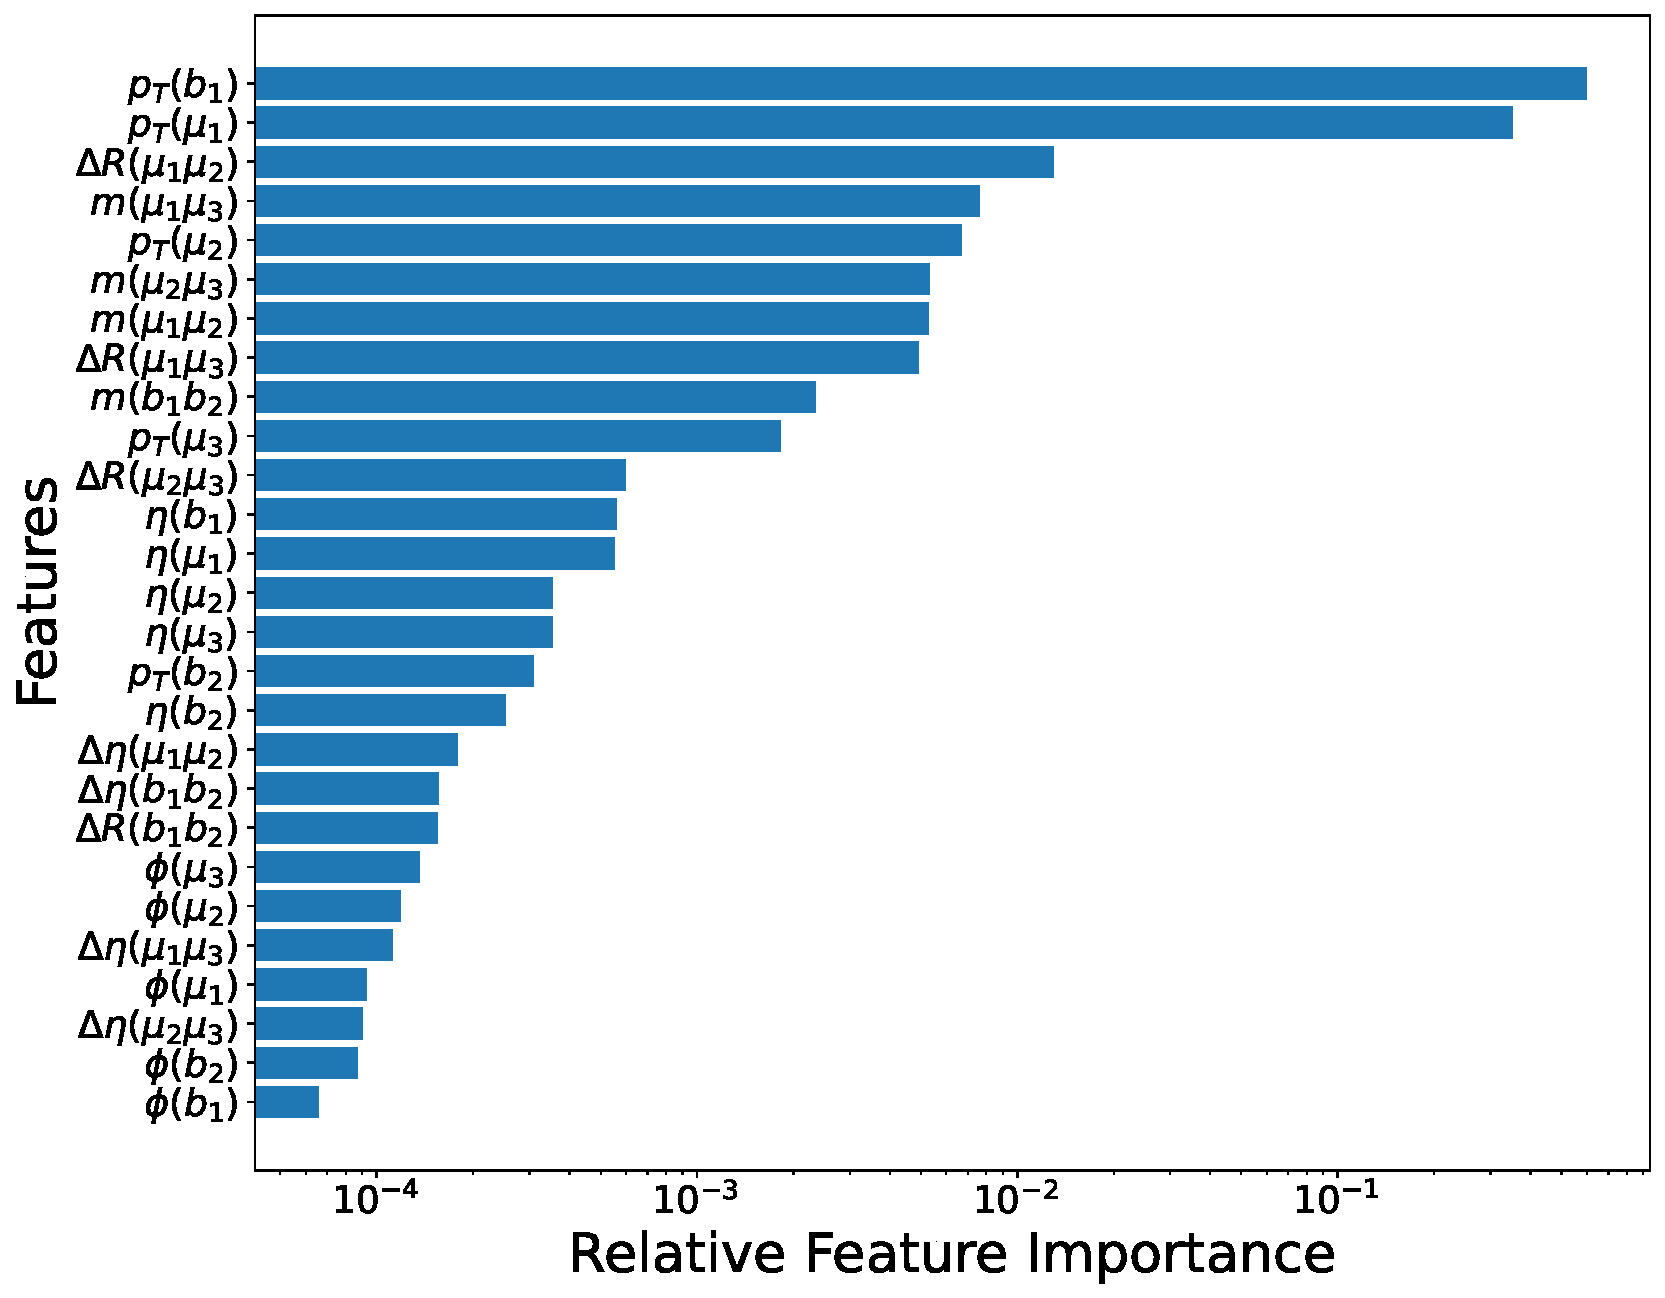
\includegraphics[width=.85\linewidth]{Images/feature_importance.pdf}
  \caption{Relative importance of features in training for a benchmark signal scenario with $m(\phi')=325\, \mathrm{GeV}$ and $m(\chi_\mathrm{u})=2000\, \mathrm{GeV}$.}
  \label{fig:feature_importance}
\end{figure}

As mentioned above, the variables $m(\mu_{i}, \mu_{j})$ for $i, j \neq 1$ provide some additional discrimination between signal and background when the leading muons are not a $\phi'$ decay candidate. The angular separation variables, such as $\Delta R(\mu_{i}, \mu_{j})$, are designed to be sensitive to lower mass $\phi'$, since the low rest mass of those particles means they acquire more boost, and thus smaller angular separation $\Delta R$ between the muon candidates. The trained BDT returns the discriminating power of each of its inputs, and the feature importance for each variable is shown in Fig.~\ref{fig:feature_importance} for a signal benchmark point with $m(\phi')=325\, \mathrm{GeV}$ and $m(\chi_\mathrm{u})=2000\, \mathrm{GeV}$.

Fig.~\ref{fig:xgboostout} shows  the distributions for the output of the BDT algorithm, normalized to unity, for the representative signal benchmark point of $m(\phi') = 1\, \mathrm{GeV}$, $m(\chi_\mathrm{u}) = 0.5\, \mathrm{TeV}$ and the two dominant backgrounds. The output of the BDT algorithm is a value between 0 and 1, which quantifies the likelihood that an event is either background-like (BDT output near $1$) or signal-like (BDT output near $0$). Fig.~\ref{fig:ROC} illustrates the true positive rate (TPR), defined as the probability of correctly selecting signal events using the BDT output, plotted against the false positive rate (FPR), defined as the probability of incorrectly selecting background events. For example, for $m(\phi') = 100\, \mathrm{GeV}$ and $m(\chi_\mathrm{u}) = 500\, \mathrm{GeV}$, when signal events are selected at $65$\% probability, the background is selected at about $10^{-3}$ probability. We note that the primary discriminating feature between the signal and background is the boosted b-jet $p_T$ coming from the $\chi_u$ vector-like quark. The $p_T$ of said b jet increases with $m(\chi_\mathrm{u})$, peaking at around $[m(\chi_\mathrm{u}) - m(\textrm{W})] / 2$. This enhanced boost increases the separation between signal and background, improving the performance of the BDT algorithm as $m(\chi_\mathrm{u})$ increases. 

\begin{figure}
\centering
  \centering  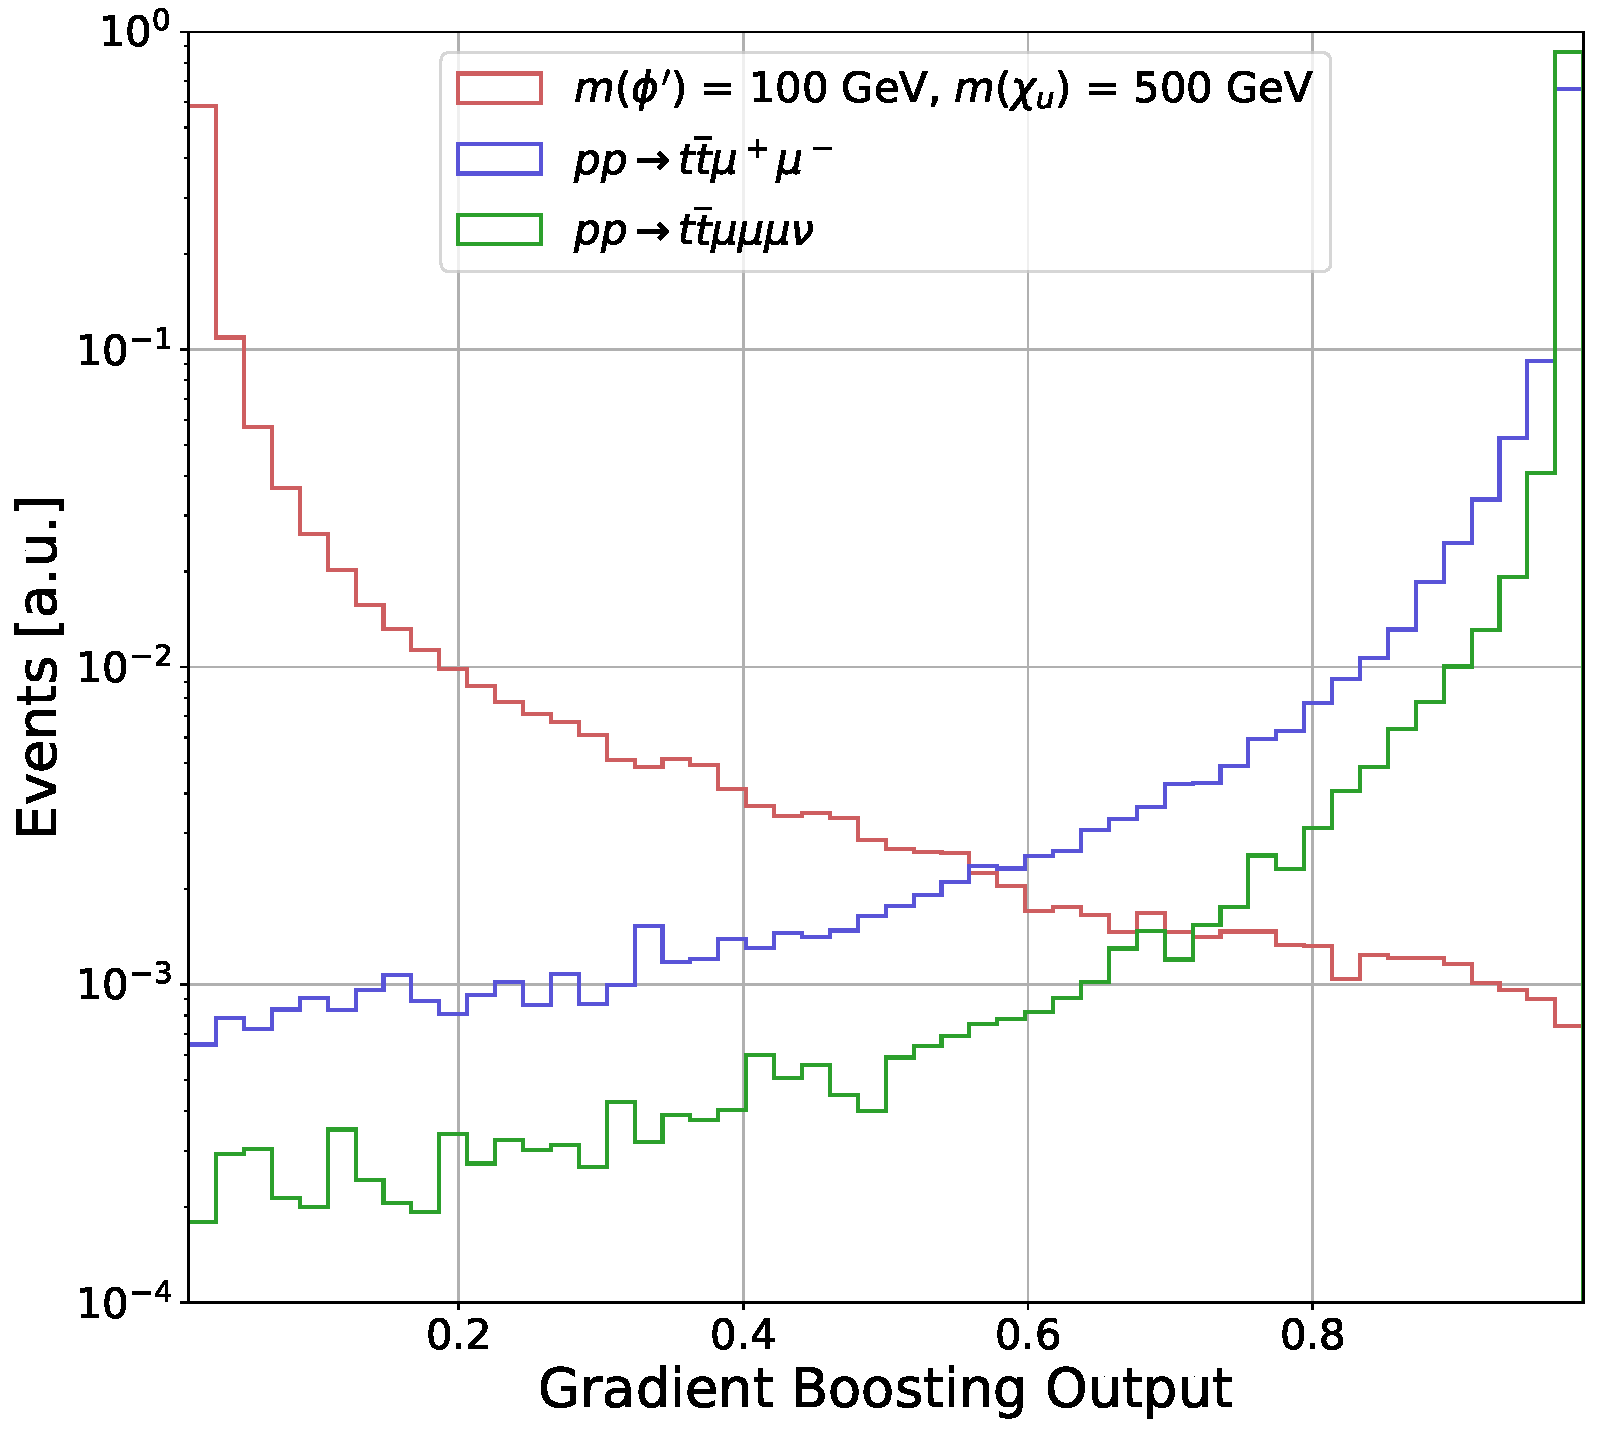
\includegraphics[width=.75\linewidth]{Images/XGB_output.pdf}
  \caption{Output of the gradient boosting algorithm for a benchmark $m(\phi') = 100$~\textrm{GeV} and $m(\chi_\mathrm{u}) = 500\, \mathrm{GeV}$ signal, and dominant backgrounds. The distributions are normalized to unity.}
  \label{fig:xgboostout}
\end{figure}


\begin{figure}
\centering
  \centering
  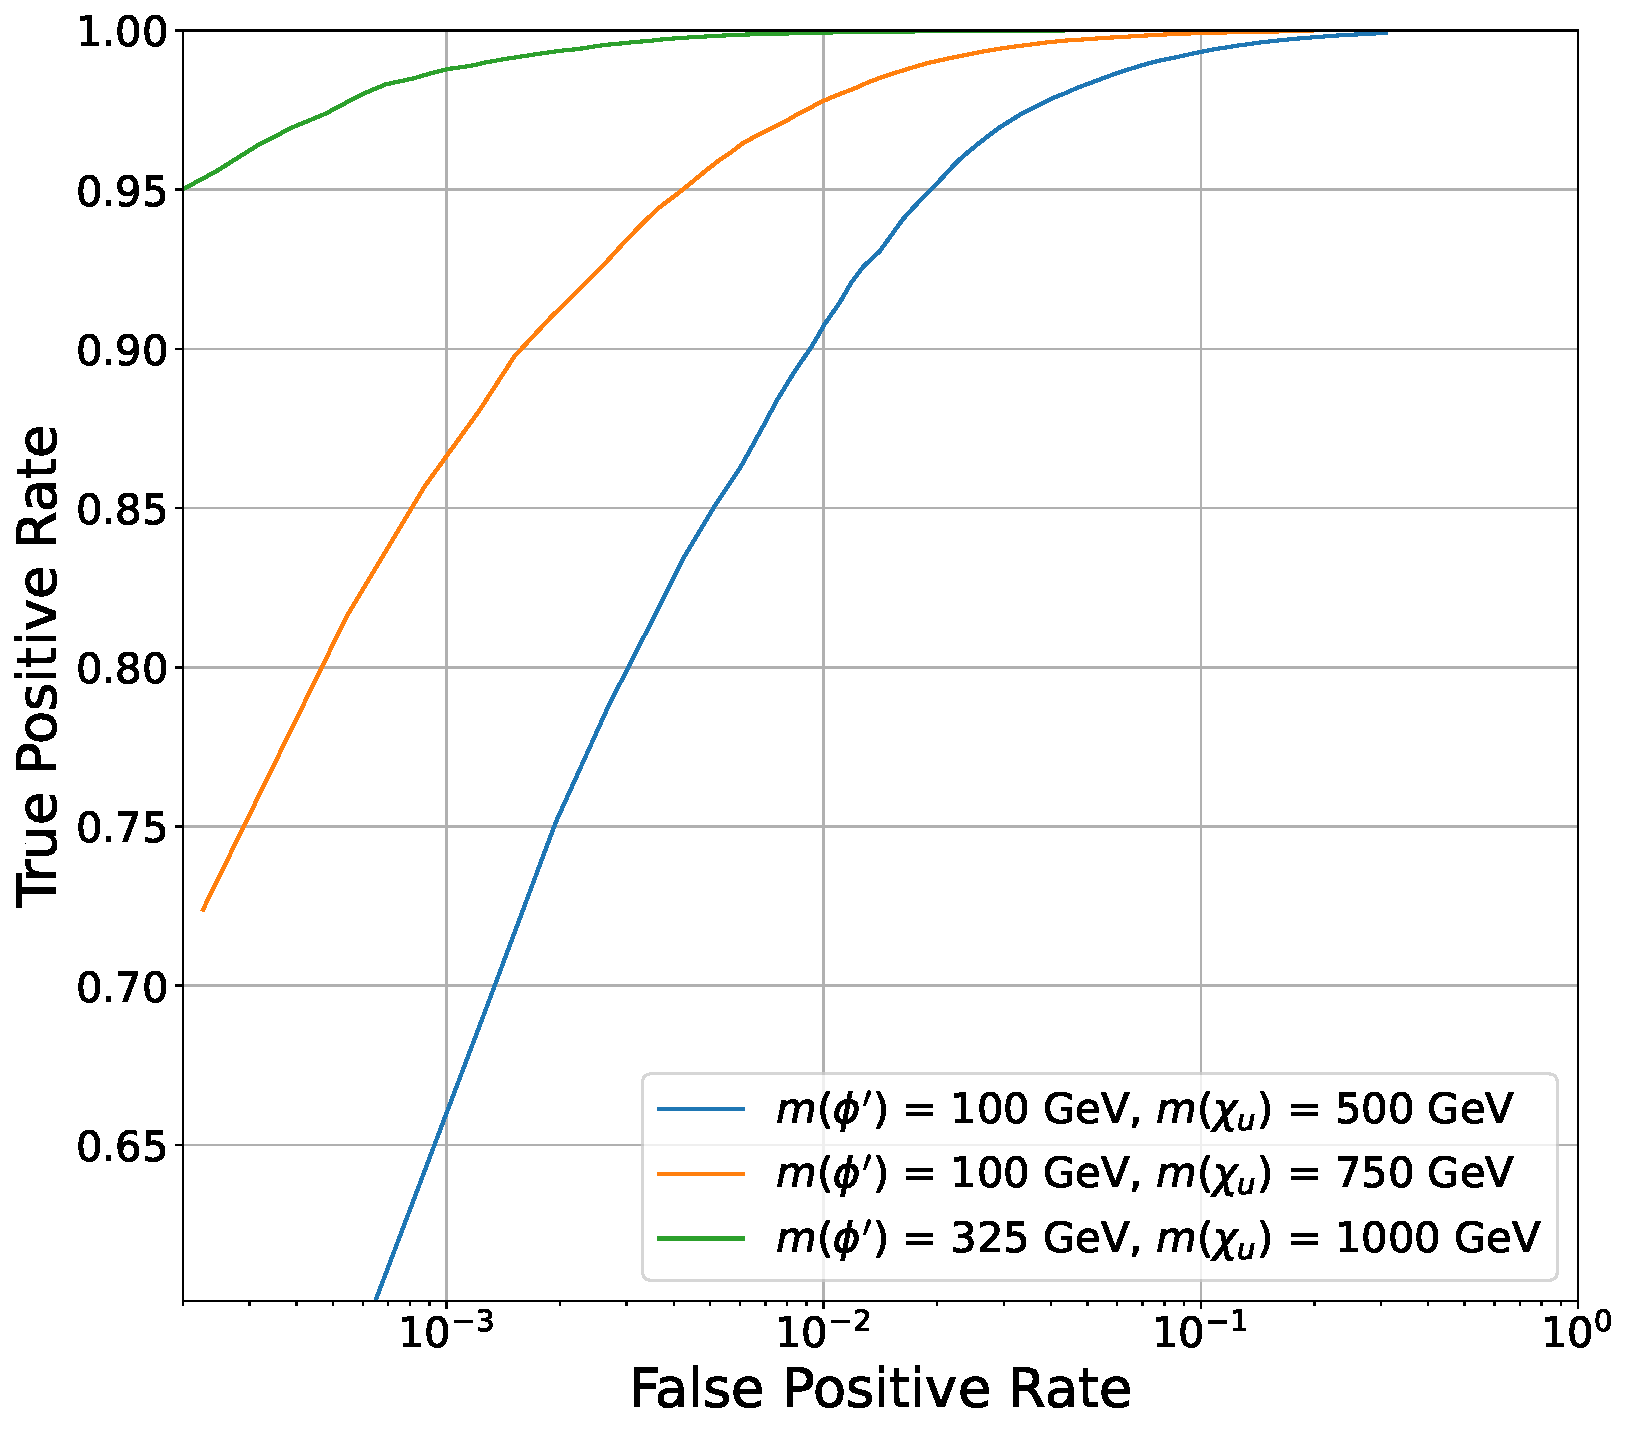
\includegraphics[width=.85\linewidth]{Images/ROC_Curve.pdf}
  \caption{Receiver operating characteristic curve of the BDT algorithm for three different signal benchmark scenarios.}
  \label{fig:ROC}
\end{figure}


The outputs from the BDT machine learning algorithm are used to perform a profile-bin likelihood analysis to estimate the signal significance for a luminosity of $3000\,\mathrm{fb^{-1}}$, corresponding to the expected amount of collected data by the end of the LHC era. For this purpose, the BDT distributions are normalized to cross section times pre-selection efficiency times luminosity for the different signal models. The significance is then calculated using the expected bin-by-bin yields of the BDT output distribution in a profile likelihood fit, using the ROOTFit~\parencite{Butterworth:2015oua} package developed by CERN. The expected signal significance $Z_\text{sig}$ is estimated using the probability of obtaining the same test statistic for the  signal plus background and the signal-null hypotheses, defined as the local $p$-value. Similar to Refs.~\parencite{Florez:2021zoo, Florez:2019tqr, Florez:2018ojp, Florez:2017xhf, VBFZprimePaper, Florez:2016lwi, Leonardi_2020}, the significance  corresponds to the point where the integral of a Gaussian distribution between $Z_\text{sig}$ and $\infty$ results in a value equal to the local $p$-value. The estimation of $Z_\text{sig}$ incorporates  systematic uncertainties. The uncertainty values have been included as nuisance parameters, considering lognormal priors for normalization and Gaussian priors for uncertainties associated with the modeling of the shapes similar to Refs.~\parencite{natalia2021longtermlhcdiscoveryreach, PhysRevD.103.095001}. 

The systematic uncertainties that have been included result from experimental and theoretical constraints.   A 1-5\% systematic uncertainty, depending on the simulated MC sample, has been included to account for the choice of Parton Distribution Function (PDF) set. The systematic uncertainty effect was incorporated following the PDF4LHC~\parencite{Butterworth:2015oua} recommendations. This systematic uncertainty has a small impact on the expected event yields for signal and background, but it does not affect the shape of the BDT output distribution. We additionally considered theoretical uncertainties related to the absence of higher-order contributions to the signal cross sections, which can change the pre-selection efficiencies and the shapes of kinematic variables used as inputs to the BDT algorithm. This uncertainty was calculated by varying the renormalization and factorization scales by $\times 2$, and studying the resulting change in the bin-by-bin yields of the BDT distributions. They are found to be at most $2$\% in a given bin. 
%Additional theoretical uncertainties were taken into account, including the potential impact of higher-order contributions to the signal cross sections. These contributions can influence the pre-selection efficiency and shapes of kinematic distributions utilized by the BDT algorithm. The uncertainty associated with this is determined by adjusting the renormalization and factorization scales by a factor of two relative to the nominal value and considering the complete change in the bin-by-bin yields of the BDT output distribution. The maximum impact of these uncertainties in a given bin is found to be 1-3\%. 

Regarding experimental uncertainties, following experimental measurements from CMS on the estimation of the integrated luminosity, a conservative $3$\% effect has been included~\parencite{lumiRef}. A $5$\% systematic uncertainty associated with the reconstruction and identification of $\mathrm{b}$-quark jets has been included, independent of $p_\mathrm{T}$ and $\eta$ of the $\mathrm{b}$-jet candidates. According to Ref.~\parencite{CMSbtag}, this uncertainty is correlated between signal and background processes with genuine  \textrm{b}-jets and is also correlated across BDT bins for each process. For muons, we include a $2$\% uncertainty associated with the reconstruction, identification, and isolation requirements, and a $3$\% systematic uncertainty to account for scale and resolution effects on the momentum and energy measurement. 
%For muon reconstruction, identification, and isolation requirements, there is a 1-2\% uncertainty, while a 1-3\% systematic uncertainty is applied to variations in energy/momentum scale and resolution. 
We consider jet energy scale uncertainties ranging from $2-5$\%, contingent on $\eta$ and $p_\mathrm{T}$, resulting in shape-based uncertainties on the BDT output distribution. Jet energy scale uncertainties were assumed to range from $1-5$\%, contingent on $\eta$ and $p_\mathrm{T}$. These assumptions lead to shape-based uncertainties on the BDT output distribution, varying from $1-2$\%. Additionally, we include  a $10$\% systematic uncertainty to account for errors in the signal and background predictions. Considering all the various sources of systematic uncertainties, our conservative  estimate yields a total effect of about $20$\%. 

\begin{figure}[]
\centering
  \centering
  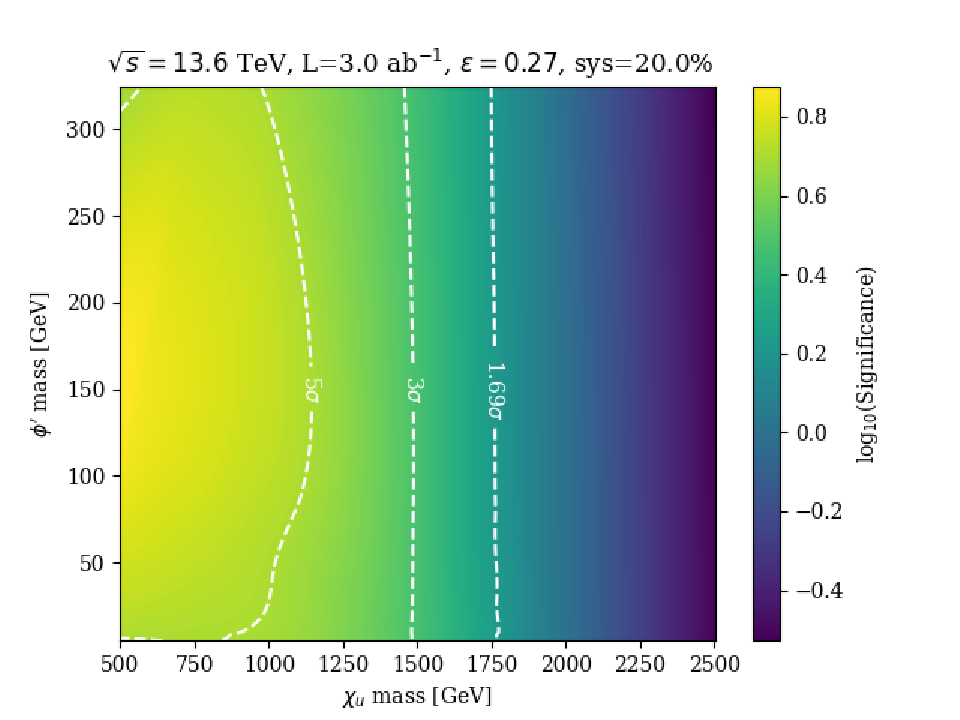
\includegraphics[width=.95\linewidth]{Images/significance.pdf}
  \caption{Signal significance for the high luminosity LHC era, considering with $3000$  $\mathrm{fb}^{-1}$ of collected data.}
  \label{fig:/significance_3000}
\end{figure}

Fig.~\ref{fig:/significance_3000} shows the expected signal significance considering an integrated luminosity of $3000$ $\mathrm{fb^{-1}}$. The significance is shown as a heat map in a two-dimensional plane for different $\phi'$ and $\chi_{\mathrm{u}}$ masses. The x-axis corresponds to $m(\chi_\mathrm{u})$, the y-axis to $m(\phi')$, and the heat map to log$_{10}(\mathrm{Z}_{sig})$. The white dashed lines are contours of constant signal significances of $1.69 \sigma$,  $3\sigma$ and  $5\sigma$ to represent regions of possible exclusion, evidence of new physics, and discovery, respectively. Under these conditions, $\phi'$ ($\chi_{\mathrm{u}}$) masses ranging from $1$ to $325$ \textrm{GeV} ($500$ to $1800$ \textrm{GeV}) can be probed. The range for a discovery with $5\sigma$ signal significance varies from $\chi_{\mathrm{u}}$ masses from $m(\chi_{\mathrm{u}}) = 770$-$1100$ \textrm{GeV}, depending  $m(\phi^{'})$. For large $m(\chi_\mathrm{u})$, the significance is almost independent of $m(\phi')$ because the primary discriminating feature—the boosted $b$-quark originating from $\phi'$—is driven predominantly by the large $m(\chi_\mathrm{u})$, with the kinematic impact of $m(\phi')$ being relatively negligible.



\section{Discussion}\label{sec:discussion}

The LHC will continue to run with pp collisions at $\sqrt{s} = 13.6$~\textrm{TeV} for the next decade. Given the increase in the integrated luminosity expected from the high-luminosity program, it is important to consider unexplored new physics phase space that diverges from the conventional assumptions made in many BSM theories, and which could have remained hidden in processes that have not yet been thoroughly examined. It is additionally crucial to explore advanced analysis techniques, in particular the use of artificial intelligence algorithms, to enhance the probability of detecting these rare corners where production cross sections are lower and discrimination from SM backgrounds is difficult. 

In this work, we examine a model based on a $U(1)_{T^3_R}$ extension of the SM, which can address various conceptual and experimental issues with the SM, including the mass hierarchy between generations of fermions, the thermal dark matter abundance, and the muon $g - 2$, $R_{(D)}$, and $R_{(D^*)}$ anomalies. This model contains a light scalar boson $\phi'$, with potential masses below the electroweak scale, and~\textrm{TeV}-scale vector-like quarks $\chi_\mathrm{u}$. We consider the scenario where the scalar $\phi'$ has family non-universal fermion couplings and $m(\phi') \ge 1$~\textrm{GeV}, as was suggested in Ref.~\cite{Dutta2020}, and thus the $\phi^{\prime}$ can primarily decay to a pair of muons. Previous works in Refs.~\cite{Dutta2023, Banerjee_2016} considered scenarios motivating a search methodology with a merged diphoton system from $\phi' \to \gamma\gamma$ decays. The authors of Ref~\cite{Dutta2023}, in which $m(\phi') < 1$~\textrm{GeV},  indeed pointed out that if the $\phi'$ is heavier than about 1~\textrm{GeV}, then decays to $\mu^+ \mu^-$ can become the preferable mode for discovery, which is the basis for the work presented in this paper. We further note that the final state topology studied in this paper would represent the most important mode for discovery at $m(\phi') < 2 m_{\mathrm{t}}$ where the $\phi' \to \mathrm{t\bar{t}}$ decay is kinematically forbidden. 

The main result of this paper is that we have shown that the LHC can probe the visible decays of new bosons with masses below the electroweak scale, down to the~\textrm{GeV}-scale, by considering the simultaneous production of heavy QCD-coupled particles, which then decay to the SM particles that contain large momentum values and can be observed in the central regions of the CMS and ATLAS detectors. The boosted system combined with innovative machine learning algorithms allows for the signal extraction above the lower-energy SM background. The LHC search strategy described here can be used to discover the prompt decay of new light particles.  An important conclusion from this paper is that the detection prospects for low-mass particles are enhanced when it is kinematically possible to simultaneously access the heavy degrees of freedom which arise in the UV completion of the low-energy model.  This specific scenario in which the couplings of the light scalars are generationally dependent, with important coupling values to the top quark, is an ideal example which would be difficult to directly probe at low energy beam experiments.

The proposed data analysis represents a competitive alternative 
to complement searches already being conducted at the LHC, allowing us to probe $\phi'$ masses from 1 to 325 \textrm{GeV}, for $m(\chi_{\mathrm{u}})$ values up to almost 2~\textrm{TeV}, at the HL-LHC. Therefore, we strongly encourage the ATLAS and CMS Collaborations to consider the proposed analysis strategy in future new physics searches.  %Vector-like quarks, p p > t t mu mu
\chapter{On Vectorial Leptoquarks Sensitivity at the LHC}\label{ch:vector_lq}

Leptoquarks ($\lq$s) are hypothetical bosons carrying both baryon and lepton number, thus interacting jointly with a lepton and a quark. They are a common ingredient in SM extensions where quarks and leptons share the same multiplet. Typical examples of these can be found in the Pati-Salam~\cite{Pati:1974yy} and $SU(5)$ GUT~\cite{Georgi:1974sy} models. In addition, they can also be found in theories with strong interactions, such as compositeness~\cite{Schrempp:1984nj}. Due to their exotic coupling which allows quark-lepton transitions, they have a diverse phenomenology, which naturally leads to several constraints. An important one comes from proton decay, which forces the $\lq$ mass to values close to the Planck scale, unless baryon and lepton numbers are not violated. Furthermore, in models where the latter are conserved, the $\lq$ can still be subject to a wide variety of bounds~\cite{Leurer:1993em,Davidson:1993qk,Leurer:1993qx,Hewett:1997ce,Queiroz:2014pra,Dorsner:2016wpm}. Examples of these come from meson mixing, electric and magnetic dipole moments, atomic parity violation tests, rare decays, and direct searches. Nevertheless, the significance of each bound is a model dependent question.
 
In the last years, an increased interest in low scale $\lq$s has emerged due to the anomalies in the precision measurements of the $\Bm$-meson decay rates. As it is well known, these corresponded mainly to deviations in the $R_{K^{(*)}}$~\cite{LHCb:2014vgu,LHCb:2017avl,LHCb:2019hip,LHCb:2021trn} and $R_{D^{(*)}}$~\cite{BaBar:2012obs,BaBar:2013mob,Abdesselam:2019dgh, Hirose:2017dxl, Sato:2016svk, Hirose:2016wfn, Huschle:2015rga,LHCb:2015gmp,Aaij:2015yra,Aaij:2017uff,LHCb:2017rln,LHCb:2023zxo} ratios, which measure the violation of lepton flavour universality (LFU). What followed was a very intense theoretical development, aiming to explain the anomalies by $\tev$ scale $\lq$ exchange at tree level~\cite{Hiller:2014yaa,Gripaios:2014tna,Alonso:2015sja,Calibbi:2015kma,Fajfer:2015ycq,Bauer:2015knc,Becirevic:2016oho,Crivellin:2017zlb,DAmico:2017mtc,Hiller:2017bzc,Buttazzo:2017ixm,Becirevic:2018afm,Cornella:2019hct,Angelescu:2021lln,Belanger:2021smw,GINO_2022}. Before the end of 2022, it was generally agreed that, within proposed single $\lq$ solutions, the only candidate capable of addressing all $\Bm$-meson anomalies simultaneously and surviving all other constraints was a vector $\lq$ ($U_1$), transforming as $({\bf 3},\,{\bf 1},\,2/3)$, and coupling mainly to third-generation fermions via $\bq\,\tau$ and $\tq\,\nu_\tau$ vertices~\cite{Buttazzo:2017ixm,Angelescu:2021lln}. In spite of a recent re-analysis of $R_{K^{(*)}}$ data showing this ratio to be compatible with the SM prediction~\cite{LHCb:2022qnv,LHCb:2022zom,Greljo:2022jac,Ciuchini:2022wbq}, the solution to the $R_{D^{(*)}}$ anomaly is still an open question and remains a valid motivation for the study of scenarios where new particles have preferential couplings to third-generation fermions. Thus, it is still of interest to continue exploring the possibility of observing the $U_1$ $\lq$ at the LHC~\cite{GINO_2022}. 

As expected, the theoretical community has extensively participated in probing $\lq$ models by scrutinizing search strategies, recasting LHC results, and predicting the reach in the parameter space via different searches involving third-generation fermions (see for instance~\cite{Diaz:2017lit,Dorsner:2018ynv,PhysRevD.99.035021,Schmaltz:2018nls,Biswas:2018snp,Baker:2019sli,Haisch:2020xjd,Bhaskar:2021gsy,Bernigaud:2021fwn,CompositenessGurrola}). In addition, several $13 \tev$ searches for $\lq$s decaying into $\tq/\bq$ and $\tau/\nu$ final states have been performed by the CMS~\cite{CMS:2016fxb,CMS:2017xcw,CMS:2018svy,CMS:2018qqq,CMS:2018txo,CMS:2018iye,CMS:2020wzx,CMS:2022goy,LQS_CMS_2022_results_comparison} and ATLAS~\cite{ATLAS:2019qpq,ATLAS:2020dsf,ATLAS:2021oiz,ATLAS:2021yij,ATLAS:2021jyv,ATLAS_7A,ATLAS_Vertical_Line} collaborations.

%Leptoquark Feynman Diagrams - fig:feynmp-prod-channels
\begin{figure}[!t]
    \centering
    %Single Leptoquark Production Diagram
    \begin{subfigure}[b]{0.45\textwidth}
        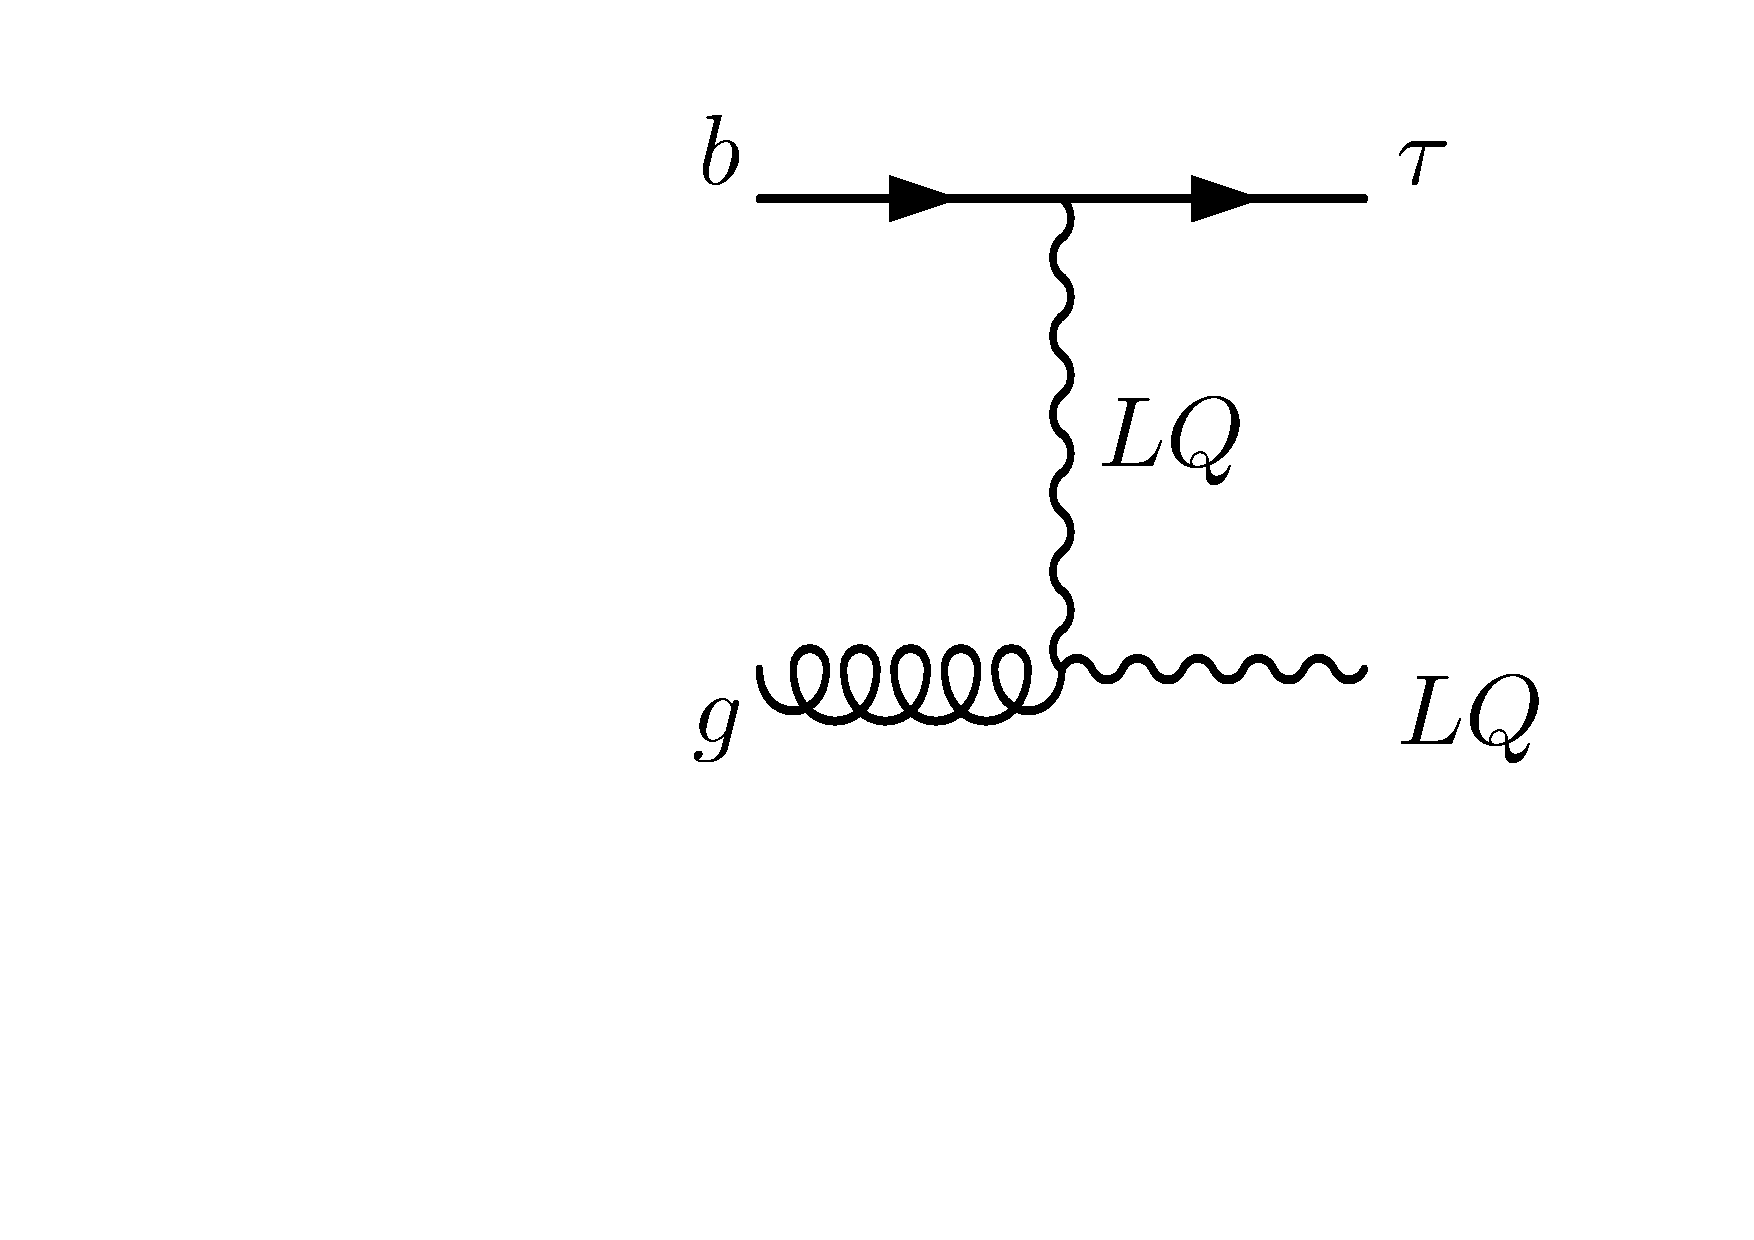
\includegraphics[width = 1.1\textwidth]{Images/feynman_diagrams/sLQ.pdf}
        \caption{}
    \end{subfigure}
    \hfill
    %Double Leptoquark Production Diagram
    \begin{subfigure}[b]{0.45\textwidth}
        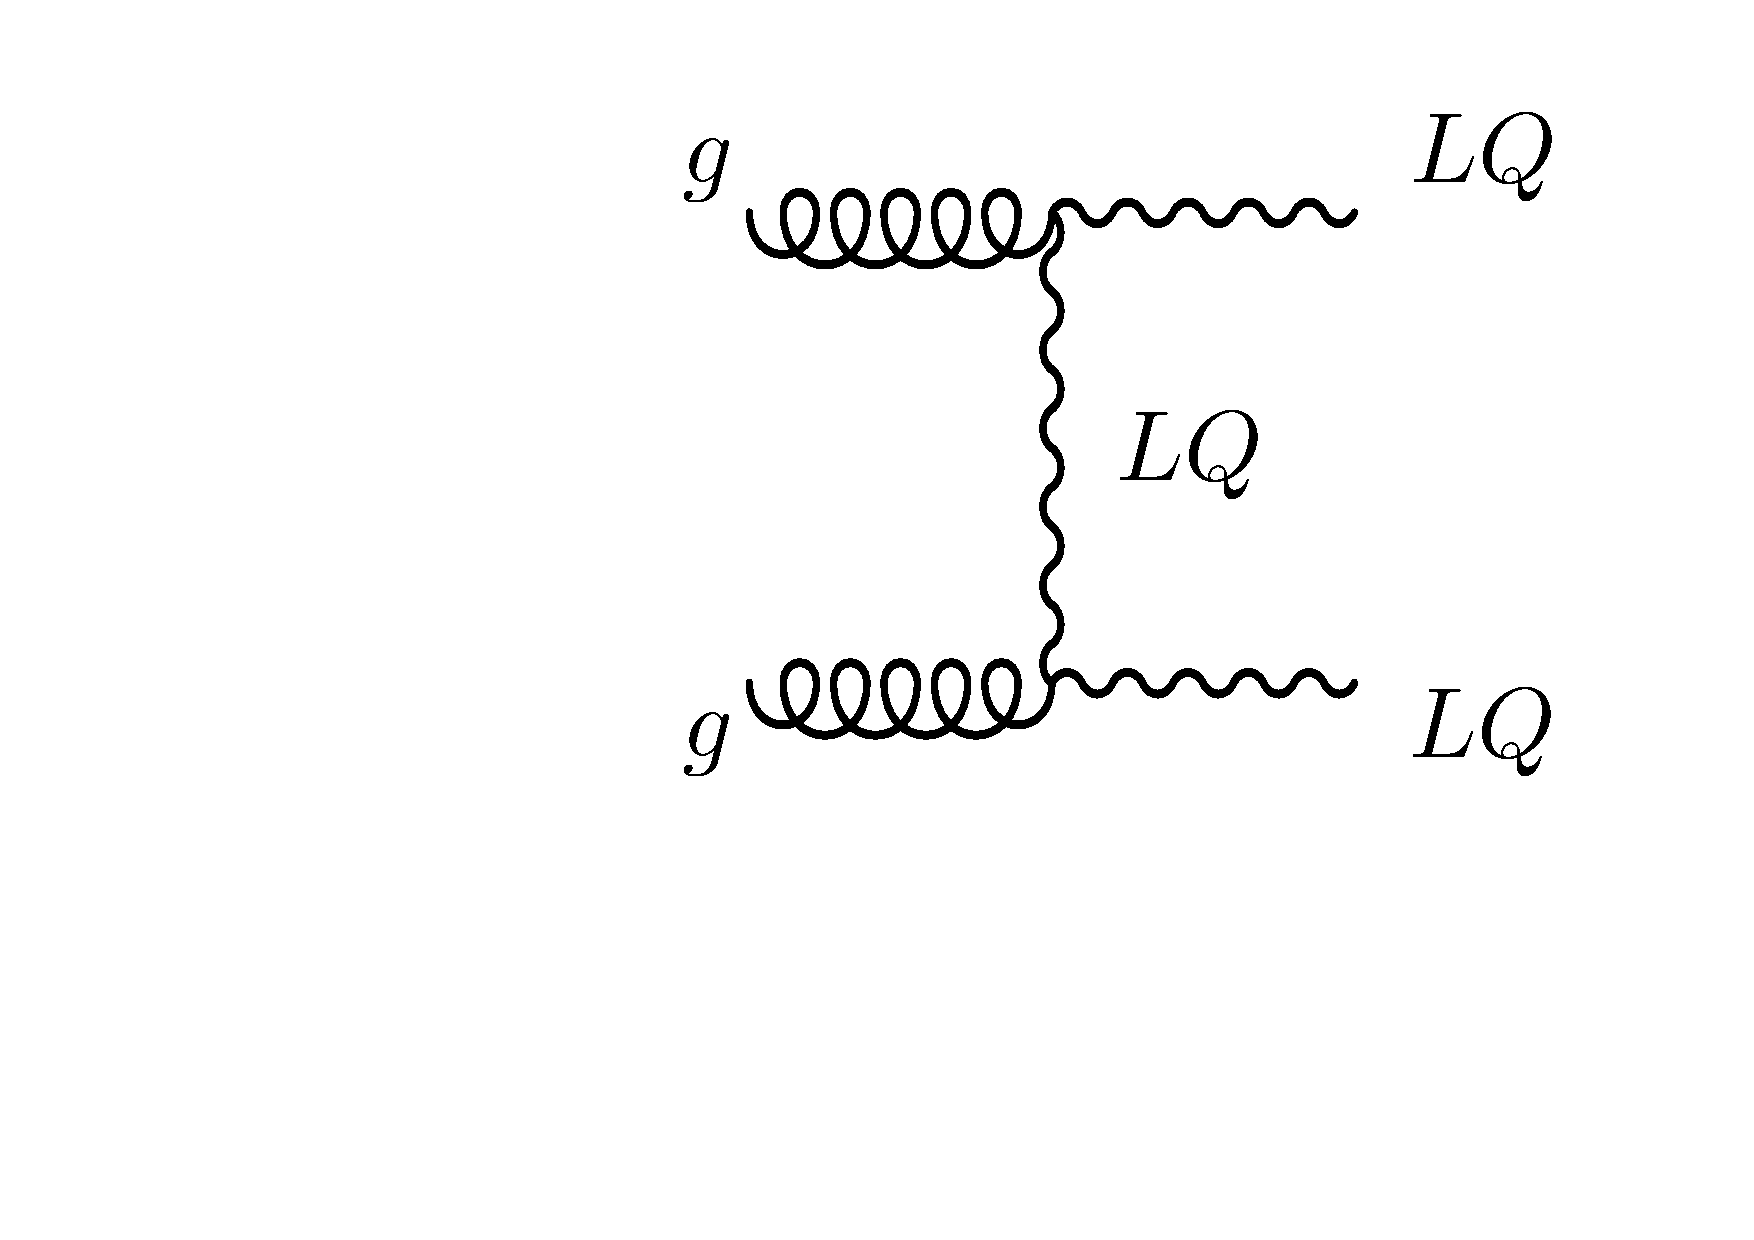
\includegraphics[width =  1.1\textwidth]{Images/feynman_diagrams/dLQ.pdf}
        \caption{}
    \end{subfigure}
    \hfill
    %non-resonant Leptoquark mediation Diagram
    \begin{subfigure}[b]{0.45\textwidth}
        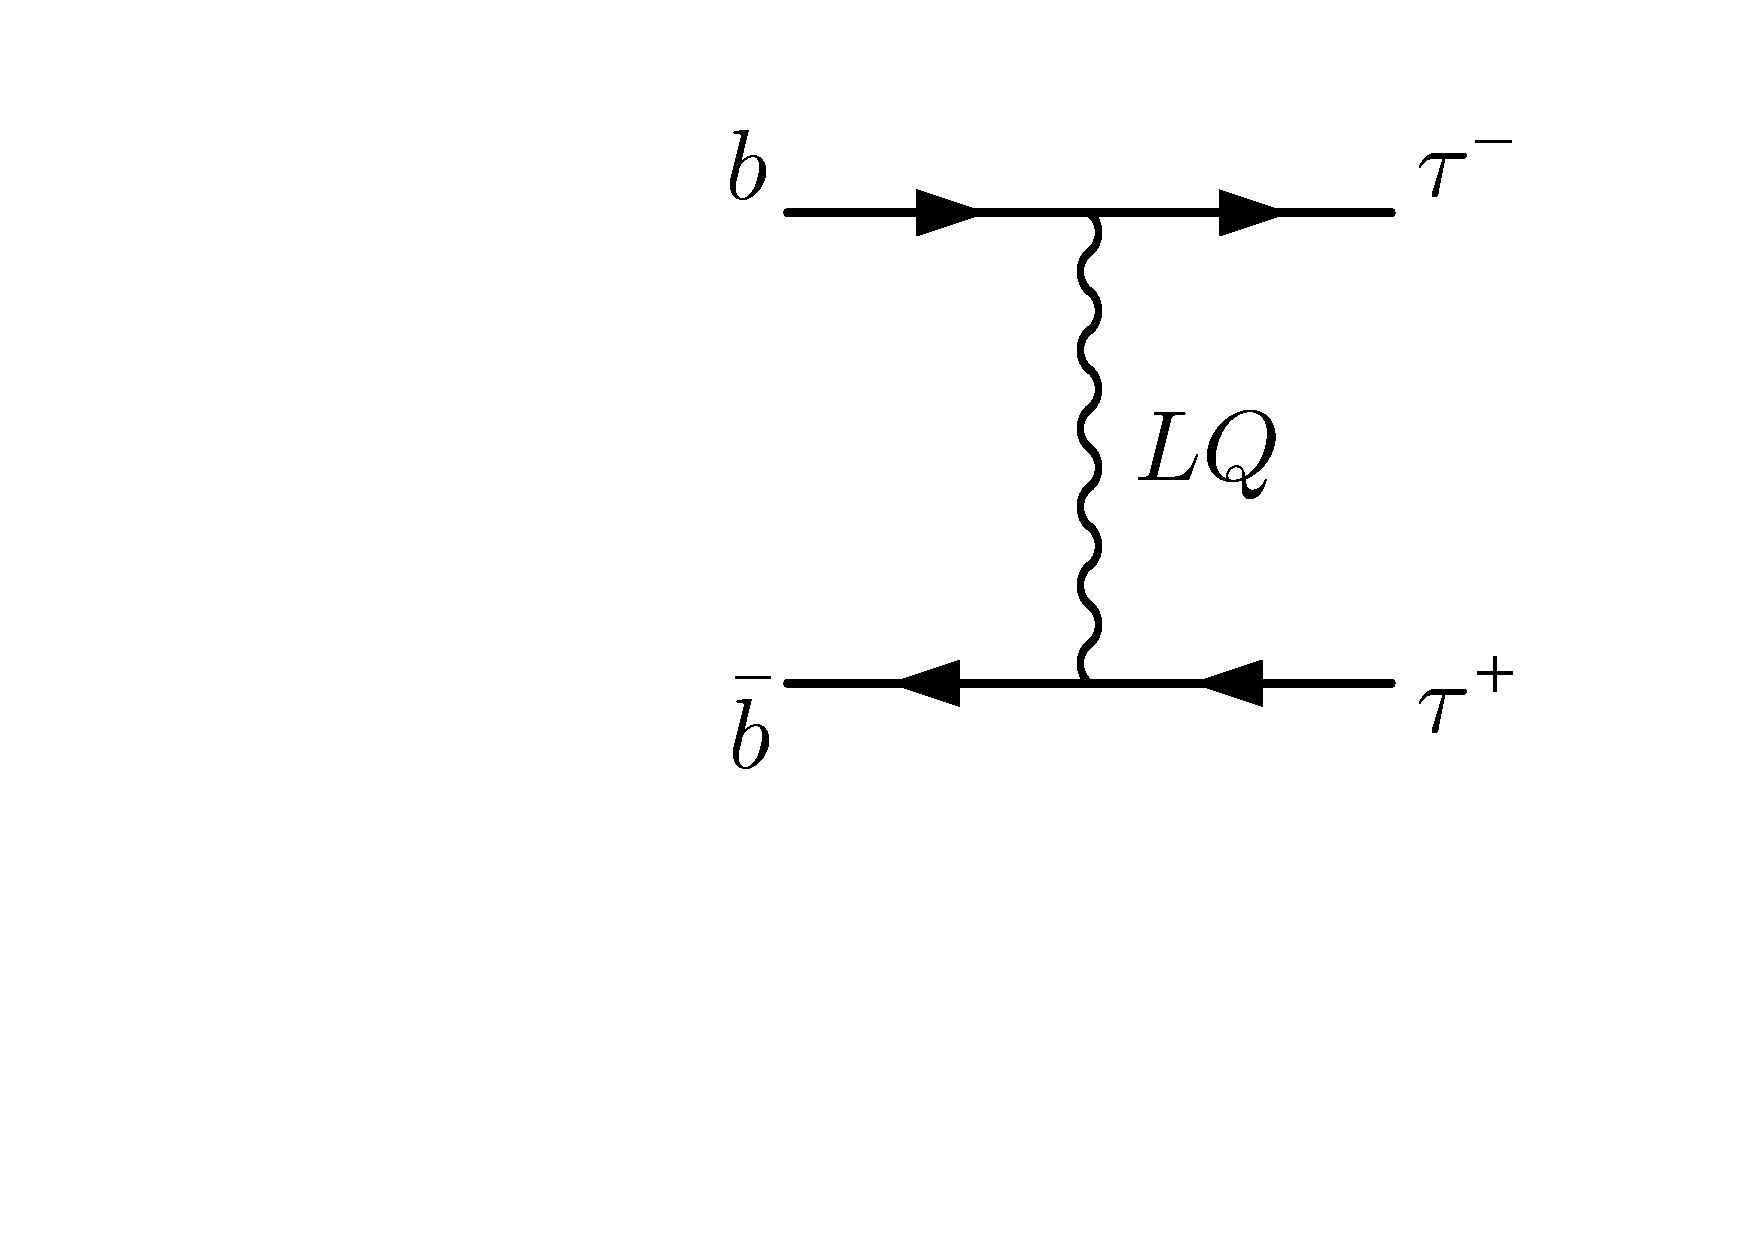
\includegraphics[width =  1.1\textwidth]{Images/feynman_diagrams/non_res.pdf}
        \caption{}
    \end{subfigure}
    \caption{Representative Feynman diagrams of single (a), pair  (b), and non-resonant (c) production leptoquarks in proton-proton collision experiments. In single and pair production, the diagrams shown involve t-channel LQ exchange, dominant for lower LQ mass. However, for larger mass there exist s-channel diagrams featuring a virtual bottom quark and gluon, respectively.}
    \label{fig:feynmp-prod-channels}
\end{figure}

Of the searches above, we find~\cite{CMS:2020wzx} particularly interesting. Here, the CMS collaboration explores signals corresponding to $\tq\,\nu\,\bq\,\tau$ and $\tq\,\nu\,\tau$ final states, with $137 \fb^{-1}$ of proton-proton ($\mathrm{p}\,\mathrm{p}$) collision data. The former is motivated by $\lq$ pair production, with one $\lq$ decaying into $\tq\,\nu$ and the other into $\bq\,\tau$, while the latter arises from a single $\lq$ produced in association with a $\tau$, with a subsequent $\lq$ decay into $\tq\,\nu$ (see Figure~\ref{fig:feynmp-prod-channels} for the corresponding diagrams). From the combination of both production channels, the search excludes $U_1$ masses under $1.3-1.7 \tev$, with this range depending on the $U_1$ coupling to gluons and on its coupling $g_U$ in the $\bq_L\,\tau_L$ vertex.

What makes this search particularly attractive is that, for the first time, an LHC collaboration directly places (mass dependent) bounds on $g_U$. This is important, since having information on this parameter is crucial in order to understand if the $U_1$ is really responsible for the $R_{D^{(*)}}$ anomaly. The inclusion of the single-$\lq$ production mode is important, since its cross-section is directly proportional to $g^2_U$. However, as can be seen in Figure~6 of~\cite{CMS:2020wzx}, the current constraints are dominated by pair production, with single-$\lq$ production playing a subleading role. While this is expected~\cite{Schmaltz:2018nls}, it still leads us to ponder the possibility of improving the sensitivity of LHC searches to single-$\lq$ production, and thus on achieving better constraints on $g_U$. Other complementary and similar searches to~\cite{CMS:2020wzx} were carried out by both ATLAS~\cite{ATLAS_7A} and CMS~\cite{LQS_CMS_2022_results_comparison}.

It is also well known, though, that searches for an excess in the high-$\pt$ tails of $\tau$ lepton distributions can strongly probe $g_U$, up to very large $\lq$ masses. Indeed, as shown in~\cite{Faroughy:2016osc,GINO_2022}, the new physics effective operators contributing to $R_D{^{(*)}}$ also contribute to an enhancement in the $\mathrm{p}\,\mathrm{p}\to\tau\tau$ production rates. This has motivated a large number of recasts~\cite{Angelescu:2018tyl,Schmaltz:2018nls,Baker:2019sli,Bhaskar:2021pml,Angelescu:2021lln,Cornella:2021sby,Allwicher:2022gkm,Haisch:2022afh,GINO_2022}, as well as a CMS search explicitly providing constraints in terms of $U_1$~\cite{CMS:2022goy}. Nevertheless, it is important to note that for these $\mathrm{p}\,\mathrm{p}\to\tau\tau$ processes, the $\lq$ participates non-resonantly, so contributions to the $\mathrm{p}\,\mathrm{p}\to\tau\tau$ rates and kinematic distributions from non-LQ BSM diagrams containing possible virtual particles, such as a heavy neutral vector boson $\zb'$, could spoil a straightforward interpretation of any possible excess~\cite{Baker:2019sli}. Thus, it is also necessary to understand how the presence of other virtual particles can affect the sensitivity of an analysis probing $g_U$.

In this work we study the projected $\lq$ sensitivity at the LHC, considering already available $\mathrm{p}\,\mathrm{p}$ data as well as the expected amount of data to be acquired during the High-Luminosity LHC (HL-LHC) runs. We explore a proposed analysis strategy which utilizes a combination of single-, double-, and non-resonant-LQ production, targeting  final states with varying $\tau$-lepton and b-jet multiplicities. 
The studies are performed considering various benchmark scenarios for different $\lq$ masses and couplings, also taking into account distinct chiralities for the third-generation fermions in the $\lq$ vertex. We also assess the impact of a companion $\zb'$, which is typical of gauge models, in non-resonant $\lq$ probes, and find that interference effects can have a significant effect on the discovery reach. We consider this effect to be of high interest, given that non-resonant $\lq$ production can have the largest cross-section, and thus could be an important channel in terms of discovery potential.

An important aspect of this work is that the analysis strategy is developed using a machine learning (ML) algorithm based on Boosted Decision Trees (BDT)\cite{friedman_greedy_2001}. The output of the event classifier is used  to perform a profile-binned likelihood test to extract the overall signal significance for each model considered in the analysis. The advantage of using BDTs and other ML algorithms has been demonstrated in several experimental and phenomenological studies~\cite{Ai:2022qvs,Biswas:2018snp,ATLAS:2017fak,Chigusa:2022svv,Chung:2020ysf,Feng:2021eke,ttZprime}. In our studies, we find that the BDT algorithm gives sizeable improvement in signal significance.

\section{A Simplified Model for the $U_1$ Leptoquark}
\label{sec:model}

Extending the SM with a massive $U_1$ vector $\lq$ is not straightforward, as one has to ensure the renormalizability of the model. Most of the theoretical community has focused on extensions of the Pati-Salam (PS) models which avoid proton decay, such as the scenario found in~\cite{Assad:2017iib}. Other examples include PS models with vector-like fermions~\cite{Calibbi:2017qbu,Blanke:2018sro,Iguro:2021kdw}, the so-called 4321 models~\cite{DiLuzio:2017vat,Greljo:2018tuh,DiLuzio:2018zxy}, the twin PS$^2$ model~\cite{King:2021jeo,FernandezNavarro:2022gst}, the three-site PS$^3$ model~\cite{Bordone:2017bld,Bordone:2018nbg,Fuentes-Martin:2022xnb}, as well as composite PS models~\cite{Gripaios:2009dq,Barbieri:2016las,Barbieri:2017tuq}.

In what follows, we shall restrict ourselves to a simplified non-renormalizable lagrangian, understood to be embedded into a more complete model. The SM is thus extended by adding the following terms featuring the $U_1$ $\lq$:
\begin{eqnarray}
\label{eq:BasicLagrangian}
  \mathcal{L}_{U_1}&=&-\frac{1}{2}U^\dagger_{\mu\nu}U^{\mu\nu}+M_U^2\, U_{1\mu}^\dagger U_1^\mu \nonumber \\
 &&  -ig_s\,U_{1\mu}^\dagger\, T^a\, U_{1\nu}\, G^{a\mu\nu}\!\!-i\frac{2}{3}g'\,U^\dagger_{1\mu}U_{1\nu}B^{\mu\nu} \nonumber \\
 && +\frac{g_U}{\sqrt 2}[U_{1\mu}(\bar Q_3\,\gamma^\mu L_3+\beta_L^{s\tau}\,\bar Q_2\,\gamma^\mu L_3 \nonumber \\  && +\beta_{R}\,\bar b_{R}\,\gamma^\mu \tau_{R}) +{\rm h.c.}] 
\end{eqnarray}
where $U_{\mu\nu}\equiv\mathcal{D}_\mu U_{1\nu}-\mathcal{D}_\nu U_{1\mu}$, and $\mathcal{D}_\mu\equiv\partial_\mu+ig_s T^a G_\mu^a+i\tfrac{2}{3}g'B_\mu$. As evidenced by the second line above, we assume that the $\lq$ has a gauge origin \footnote{The couplings in the second line of Eq.~(\ref{eq:BasicLagrangian}) can be found in the literature as $g_s\to g_s(1-\kappa_U)$ and $g'\to g'(1-\tilde\kappa_U)$, in order to take into account the possibility of an underlying strong interaction.}.

The third and fourth lines in in Eq.~(\ref{eq:BasicLagrangian}) shows the $\lq$ interactions with SM fermions, with coupling $g_U$, which we have chosen as preferring the third generation~\footnote{Before the demise of the $R_{K^{(*)}}$ anomaly~\cite{LHCb:2022qnv,LHCb:2022zom,Greljo:2022jac,Ciuchini:2022wbq}, a $3\times3$ $\beta_L$ matrix would be used instead, with values fitted to solve all $\Bm$ meson anomalies.}. These are particularly relevant for the $\lq$ decay probabilities, as well as for the single-$\lq$ production cross-section. The $\beta_L^{s\tau}$ parameter, which is the $\lq \to s\tau$ coupling in the $\beta_L$ matrix (see footnote), is chosen to be equal to $0.2$, following the fit done in~\cite{Cornella:2021sby}, in order to simultaneously solve the $R_{D^{(*)}}$ anomaly and satisfy the $\mathrm{p}\,\mathrm{p}\to\tau^+\tau^-$ constraints. Although $\beta_L^{s\tau}$ technically alters the single-$\lq$ production cross-section and $\lq$ branching fractions, we have confirmed that a value of $\beta_L^{s\tau} = 0.2$ results in negligible impact on our collider results, and thus is ignored in our subsequent studies.

The $\lq$ right-handed coupling is modulated with respect to the left-handed one by the $\beta_R$ parameter. The choice of $\beta_R$ is important phenomenologically, as it affects the $\lq$ branching ratios \footnote{Having $\beta_L^{s\tau}$ different from zero also opens new decay channels. These, however, are either suppressed by $\beta_L^{s\tau}$ and powers of $\lambda_{\rm CKM}$. In any case, this effect would decrease ${\rm BR}(\lq \to \bq\,\tau)$ and ${\rm BR}(\lq \to \tq\,\nu)$ by less than $3\%$.}, as well as the single-$\lq$ production cross-section. To illustrate the former, Fig.~\ref{fig:branching_ratios} (top) shows the $\lq\to\textrm{b}\tau$ and $\lq\to\textrm{t}\nu$ branching ratios as functions of the $\lq$ mass, for two values of $\beta_R$. For large $\lq$ masses, we confirm that with $\beta_R = 0$ then ${\rm BR}(\lq \to \bq\,\tau) \approx {\rm BR}(\lq \to \tq\,\nu)\approx \tfrac{1}{2}$. However, for $\beta_R = -1$, as was chosen in~\cite{Cornella:2019hct}, the additional coupling adds a new term to the total amplitude, leading to ${\rm BR}(\lq\to \bq\,\tau) \approx \tfrac{2}{3}$. The increase in this branching ratio can thus weaken bounds from $\lq$ searches targeting decays into $\tq\,\nu$ final states, which motivates exploring the sensitivity in b$\tau$ final states exclusively. Note that although a ${\rm BR}(\lq\to \bq\,\tau) \approx 1$ scenario is possible by having the $\lq$ couple exclusively to right-handed currents (i.e, $g_U\to0$, but $g_U\beta_R\not=0$), it does not solve the observed anomalies in the $R_{D^{(*)}}$ ratios. Therefore, although some LHC searches assume ${\rm BR}(\lq\to \bq\,\tau) = 1$, we stress that in our studies we assume values of the model parameters and branching ratios that solve the $R_{D^{(*)}}$ ratios.
\begin{center}
    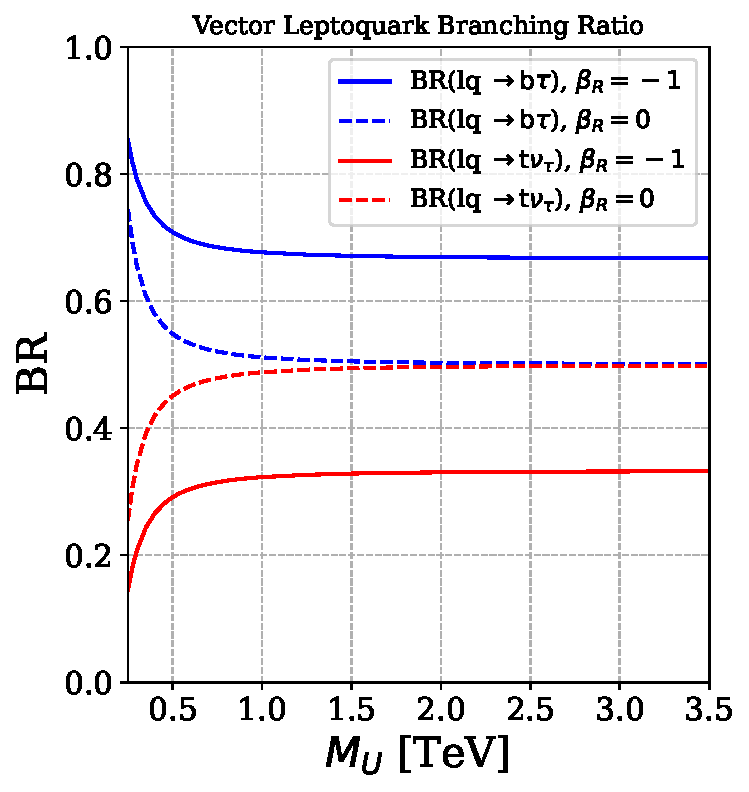
\includegraphics[width=.49\textwidth]{Images/VLQ_BranchingRatio.pdf}
    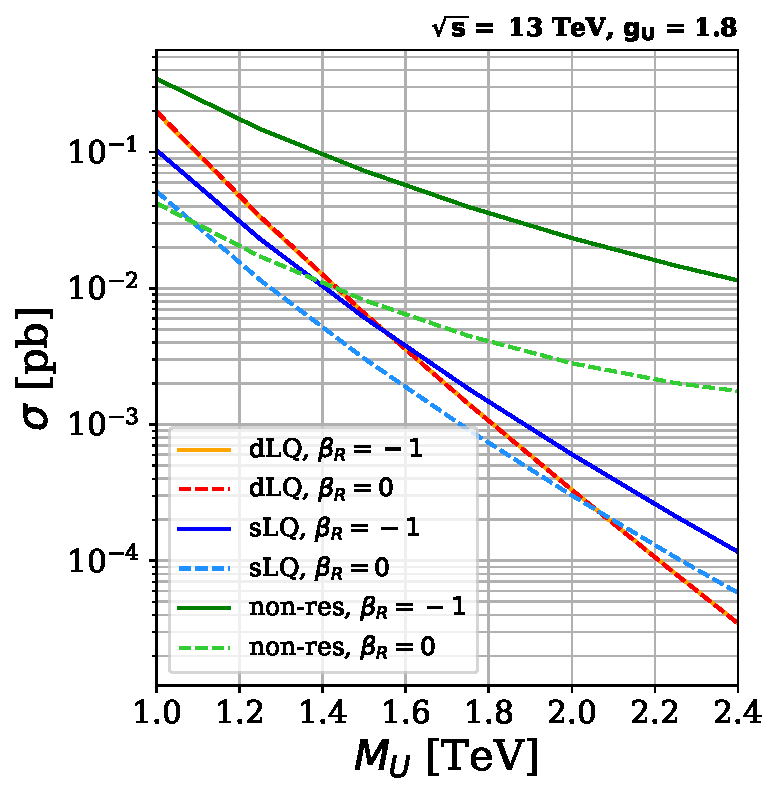
\includegraphics[width=.49\textwidth]{Images/prod_cross_section_13TeV.pdf}
    \captionof{figure}{Left: The $\lq\to\textrm{b}\tau$ and $\lq\to\textrm{t}\nu$ branching ratios for $\beta_{R} = 0$ (solid lines) and $\beta_{R} = -1$ (dashed lines). Right: Signal cross-section as a function of the $\lq$ mass, for $\sqrt{ s}=13 \tev$, with $g_U=1.8$. We show single, pair, and non-resonant production, for $\beta_R=-1,\,0$ in solid and dashed lines, respectively.}
\label{fig:branching_ratios}
\end{center}

To further understand the role of $\beta_R$ at colliders, Fig.~\ref{fig:branching_ratios} (bottom) shows the cross-section for single-$\lq$ (s$\lq$), double-$\lq$ (d$\lq$), and non-resonant (non-res) production, as a function of mass and for a fixed coupling $g_{U} = 1.8$, assuming $\mathrm{p}\,\mathrm{p}$ collisions at $\sqrt{s} = 13$ $\tev$. We note that this benchmark scenario with $g_{U}=1.8$ results in a $\lq\to\textrm{b}\tau$ decay width that is $<$5\% of the $\lq$ mass, for mass values from 250 $\gev$ to 2.5 $\tev$. In the Figure, we observe that, since d$\lq$ production is mainly mediated by events from quantum chromodynamic processes, the choice of $\beta_R$ does not affect the cross-section. However, for  s$\lq$ production, a non-zero value for $\beta_R$ increases the cross-section by about a factor of 2 and by almost one order of magnitude in the case of non-res production. These results shown in Fig.~\ref{fig:branching_ratios} are easily understood by considering the diagrams shown in Fig.~\ref{fig:feynmp-prod-channels}. The $\lq$ mass value where the s$\lq$ production cross-section exceeds the d$\lq$ cross-section depends on the choice of $g_U$. 
 
We also note that to solve the $R_{D^{(*)}}$ anomaly, the authors of~\cite{Cornella:2021sby} point out that the wilson coefficient $C_U\equiv g^2_U\,v^2_{SM}/(4\,M^2_U)$ is constrained to a specific range of values, and this range depends on the value of the $\beta_{R}$ parameter. Therefore, the allowed values of the coupling $g_{U}$ depend on $M_{U}$ and $\beta_{R}$, and thus our studies are performed in this multi-dimensional phase space.


We study the role of a $\zb'$ boson in $\mathrm{p}\,\mathrm{p}\to\tau\tau$ production. The presence of a $\zb'$ boson in $\lq$ models has been justified in various papers, for example, in~\cite{Baker:2019sli}. The argument is that minimal extensions of the SM which include a massive gauge $U_1$ LQ, uses the gauge group $SU(4)\times SU(3)^{\prime}\times SU(2)_L \times U(1)_{T_R^3}$. Such an extension implies the presence of an additional massive boson, $\zb^{\prime}$, and a color-octet vector, $G'$, arising from the spontaneous symmetry breaking into the SM, see for example App.~\cite{sec:4321}. \marginpar{Naively, the LQs are associated to the breaking of $SU(4)\to SU(3)_{[4]}\times U(1)_{B-L}$, the $G'$ arises from $SU(3)_{[4]}\times SU(3)'\to SU(3)_c$, and the $Z'$ comes from the breaking of $U(1)_{B-L}\times U(1)_{T_R^3}\to U(1)_Y$. Notice that the specific pattern of breaking, and the relations between the masses and couplings, are connected to the specific scalar potential used.}  The $\zb'$ in particular can play an important role in the projected $\lq$ discovery reach, as it can participate in $\mathrm{p}\,\mathrm{p}\to\tau\tau$ production by s-channel exchange, both resonantly and as a virtual mediator. To study the effect of a $\zb'$ on the $\mathrm{p}\,\mathrm{p}\to\tau\tau$ production cross-sections and kinematics, we extend our benchmark Lagrangian in Eq.~(\ref{eq:BasicLagrangian}) with further non-renormalizable terms involving the $\zb'$. Accordingly, we assume the $\zb'$ only couples to third-generation fermions. Our simplified model is thus extended by:
\begin{eqnarray}
    \label{eq:BasicLagrangianZp}
        \mathcal{L}_{Z^{\prime}}&= & -\frac{1}{4} Z_{\mu \nu}^{\prime} Z^{\prime \mu \nu}+\frac{1}{2} M_{Z^{\prime}}^2 Z_\mu^{\prime} Z^{\prime \mu} \nonumber \\
        && + \frac{g_{Z^{\prime}}}{2 \sqrt{6}} Z^{\prime \mu} (\zeta_q \bar{Q}_3 \gamma_\mu Q_3 \nonumber +\zeta_t \bar{t}_R \gamma_\mu t_R \\
        &&  +\zeta_b \bar{b}_R \gamma_\mu b_R-3 \zeta_{\ell} \bar{L}_3 \gamma_\mu L_3-3 \zeta_\tau \bar{\tau}_R \gamma_\mu \tau_R)
\end{eqnarray}
where the constants $M_{\zb^{\prime}}$, $g_{Z^{\prime}}$, $\zeta_q $, $\zeta_t $, $\zeta_b$, $\zeta_{\ell}$, $\zeta_\tau$, are model dependent.

We study two extreme cases for the $\zb'$ mass, following~\cite{GINO_PhysRevD.102.115015}, namely $M_{\zb'} = \sqrt{\tfrac{1}{2}}M_U<M_U$ and $M_{\zb'} = \sqrt{\tfrac{3}{2}}M_U>M_U$. We also assume the $\lq$ and $\zb'$ are uniquely coupled to left-handed currents, i.e. $\zeta_q=\zeta_\ell= 1$ and $\zeta_t=\zeta_b=\zeta_\tau=0$. With these definitions, Fig.~\ref{fig:xsinterference} shows the effect of the $\zb'$ on the $\tau\tau$ production cross-section, considering $g_U = 1$, $\beta_R=0$, and different $g_{\zb^{\prime}}$ couplings. On the left, the cross-sections corresponding to the cases where $M_{\zb'} = \sqrt{\tfrac{1}{2}}M_U$ are shown. As expected, the $\tau\tau$ production cross-section for the inclusive case (i.e., $g_{\zb'} \neq 0$) is larger than that for the $\lq$-only non-res process ($g_{\zb'} = 0$, depicted in blue). This effect increases with $g_{\zb'}$ and, within the evaluated values, can exceed the $\lq$-only cross-section by up to two orders of magnitude. In contrast, a more intricate behaviour can be seen on the right of Fig.~\ref{fig:xsinterference}, which corresponds to $M_{\zb'} = \sqrt{\tfrac{3}{2}}M_U$. Here, for low values of $M_U$, a similar increase in the cross-section is observed. However, for higher values of $M_U$, the inclusive $\mathrm{p}\,\mathrm{p}\to\tau\tau$ cross-section is smaller than the $\lq$-only $\tau\tau$ cross-section. This behaviour suggests the presence of a dominant destructive interference at high masses, leaving its imprint on the results.
\begin{center}
    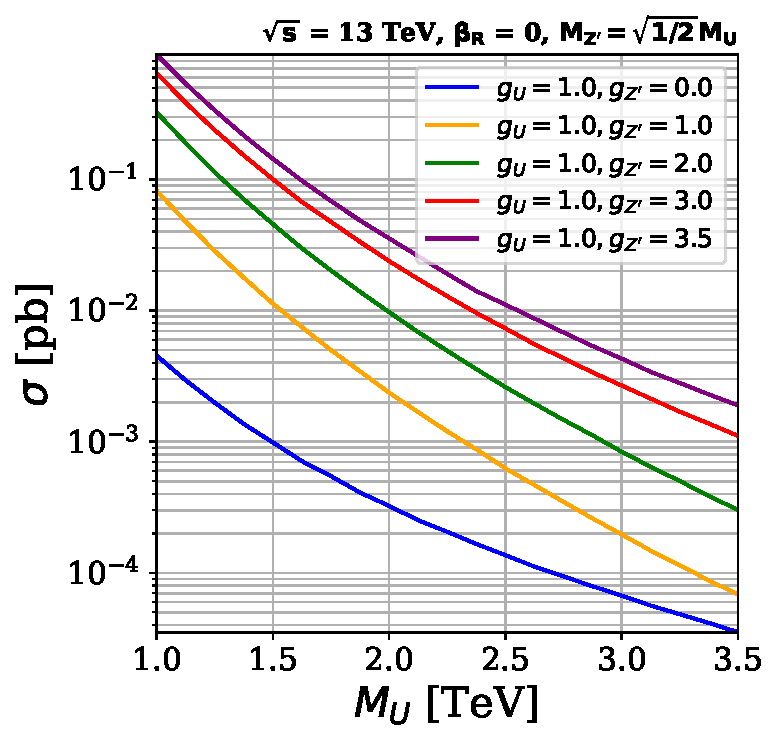
\includegraphics[width=.49\textwidth]{Images/XS_gu_gzp_lower_limit_woRHC.pdf}
    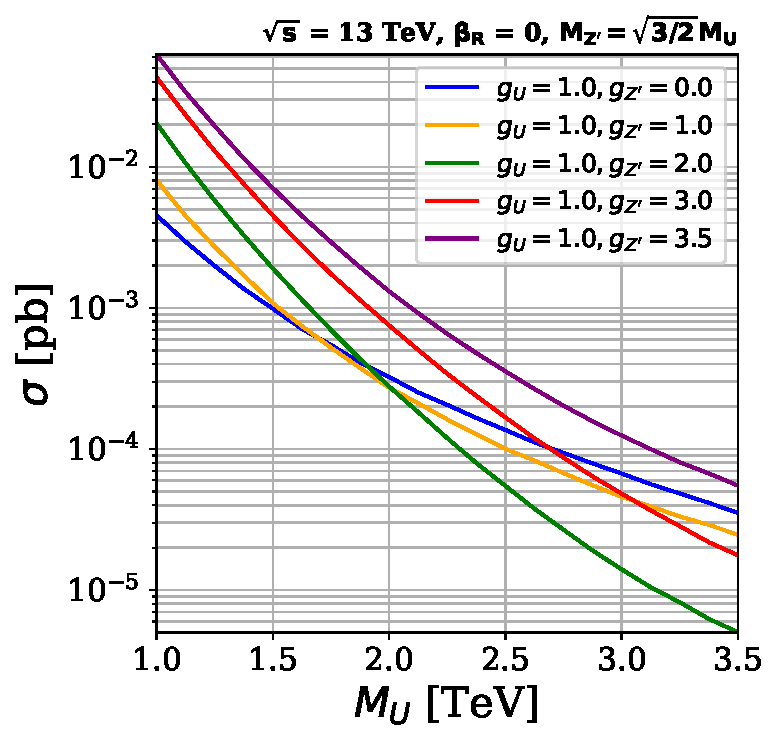
\includegraphics[width=.49\textwidth]{Images/XS_gu_gzp_upper_limit_woRHC.pdf}
    \captionof{figure}{$\tau \tau$ cross-section as a function of the $\lq$ mass for different values of $g_U$ and $g_{\zb^{\prime}}$. The estimates are performed at $\sqrt s=13 \tev$, $\beta_R=0$,  $M_{\zb^{\prime}} = \sqrt{1/2} M_{U}$ (left), and $M_{\zb^{\prime}} = \sqrt{3/2} M_{U}$ (right).}
\label{fig:xsinterference}
\end{center}

\begin{center}
    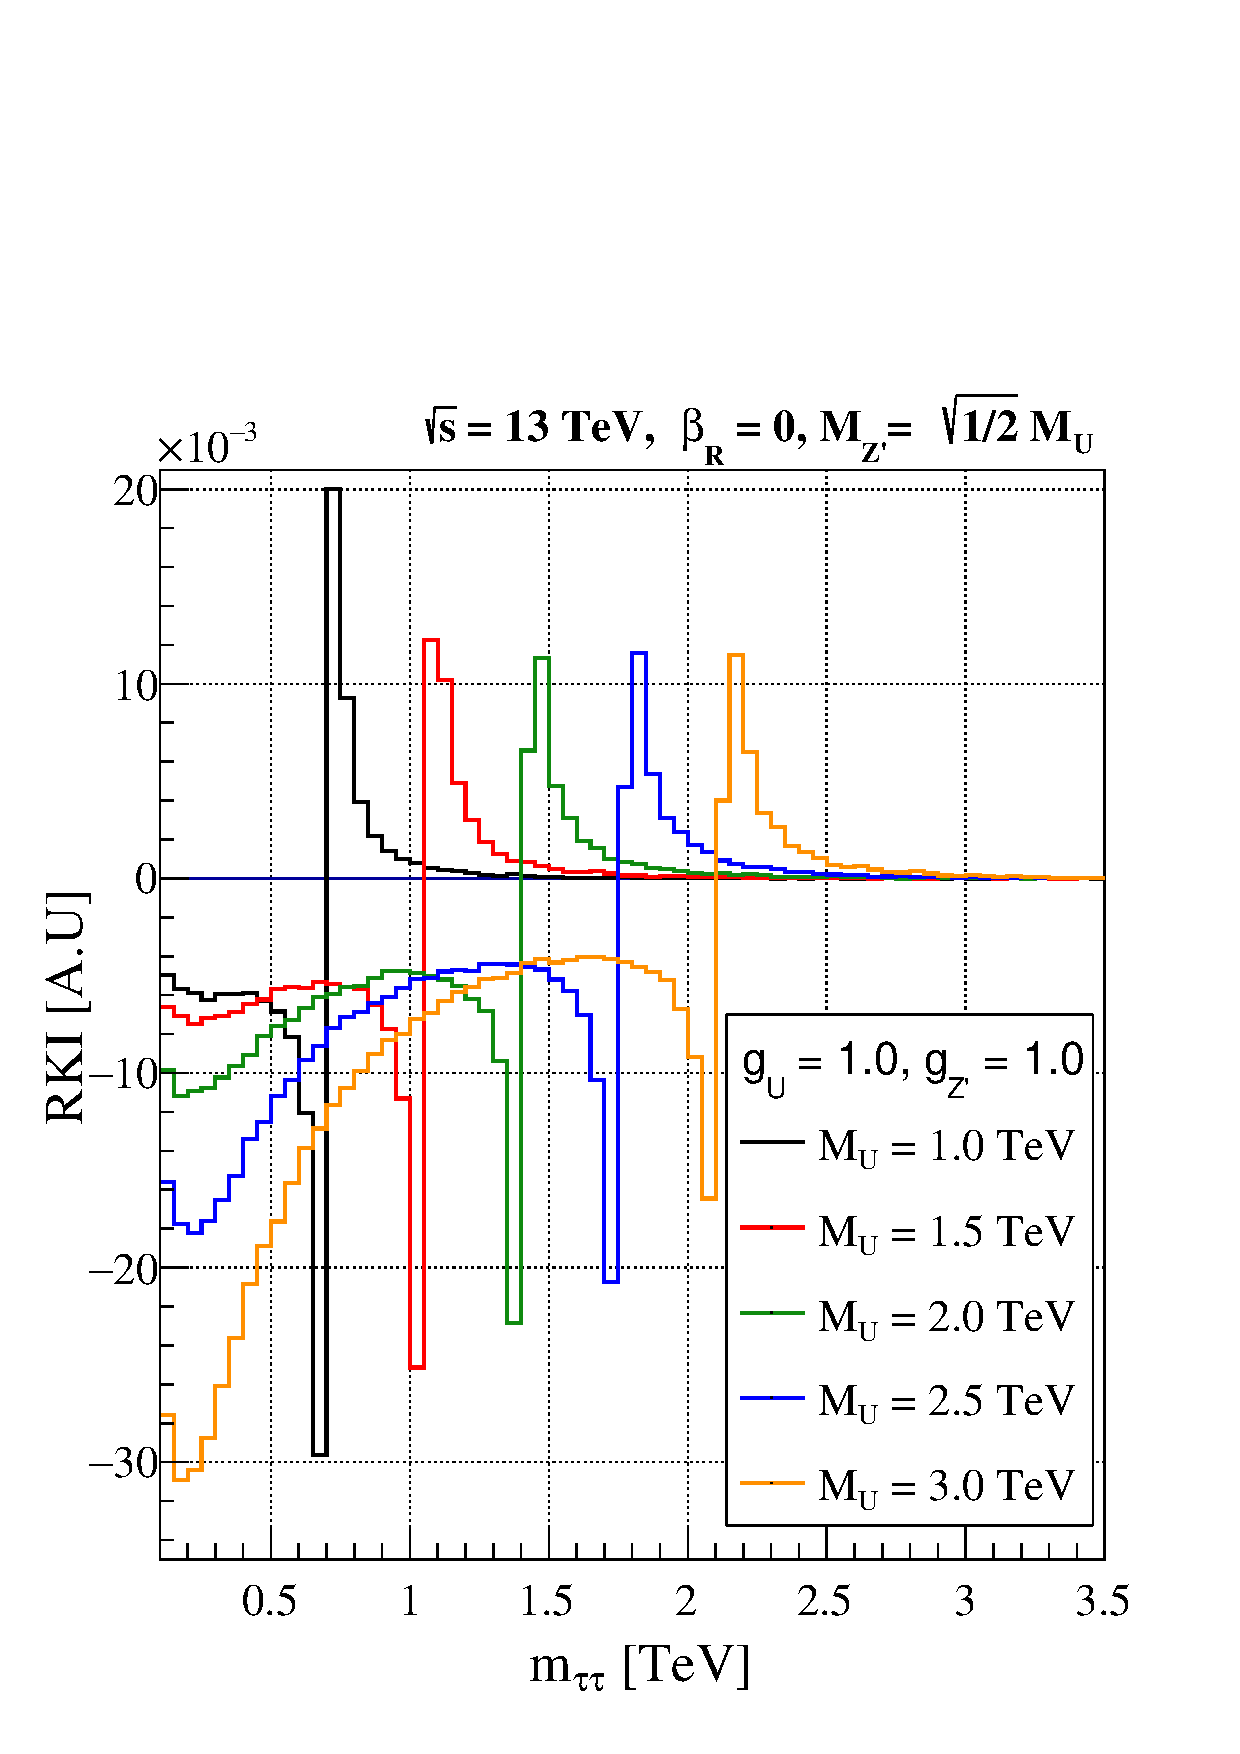
\includegraphics[width=.49\textwidth]{Images/Kinematic_Interference_gu_1.0_gzp_1.0_zp_lower_limit_woRHC.pdf}
    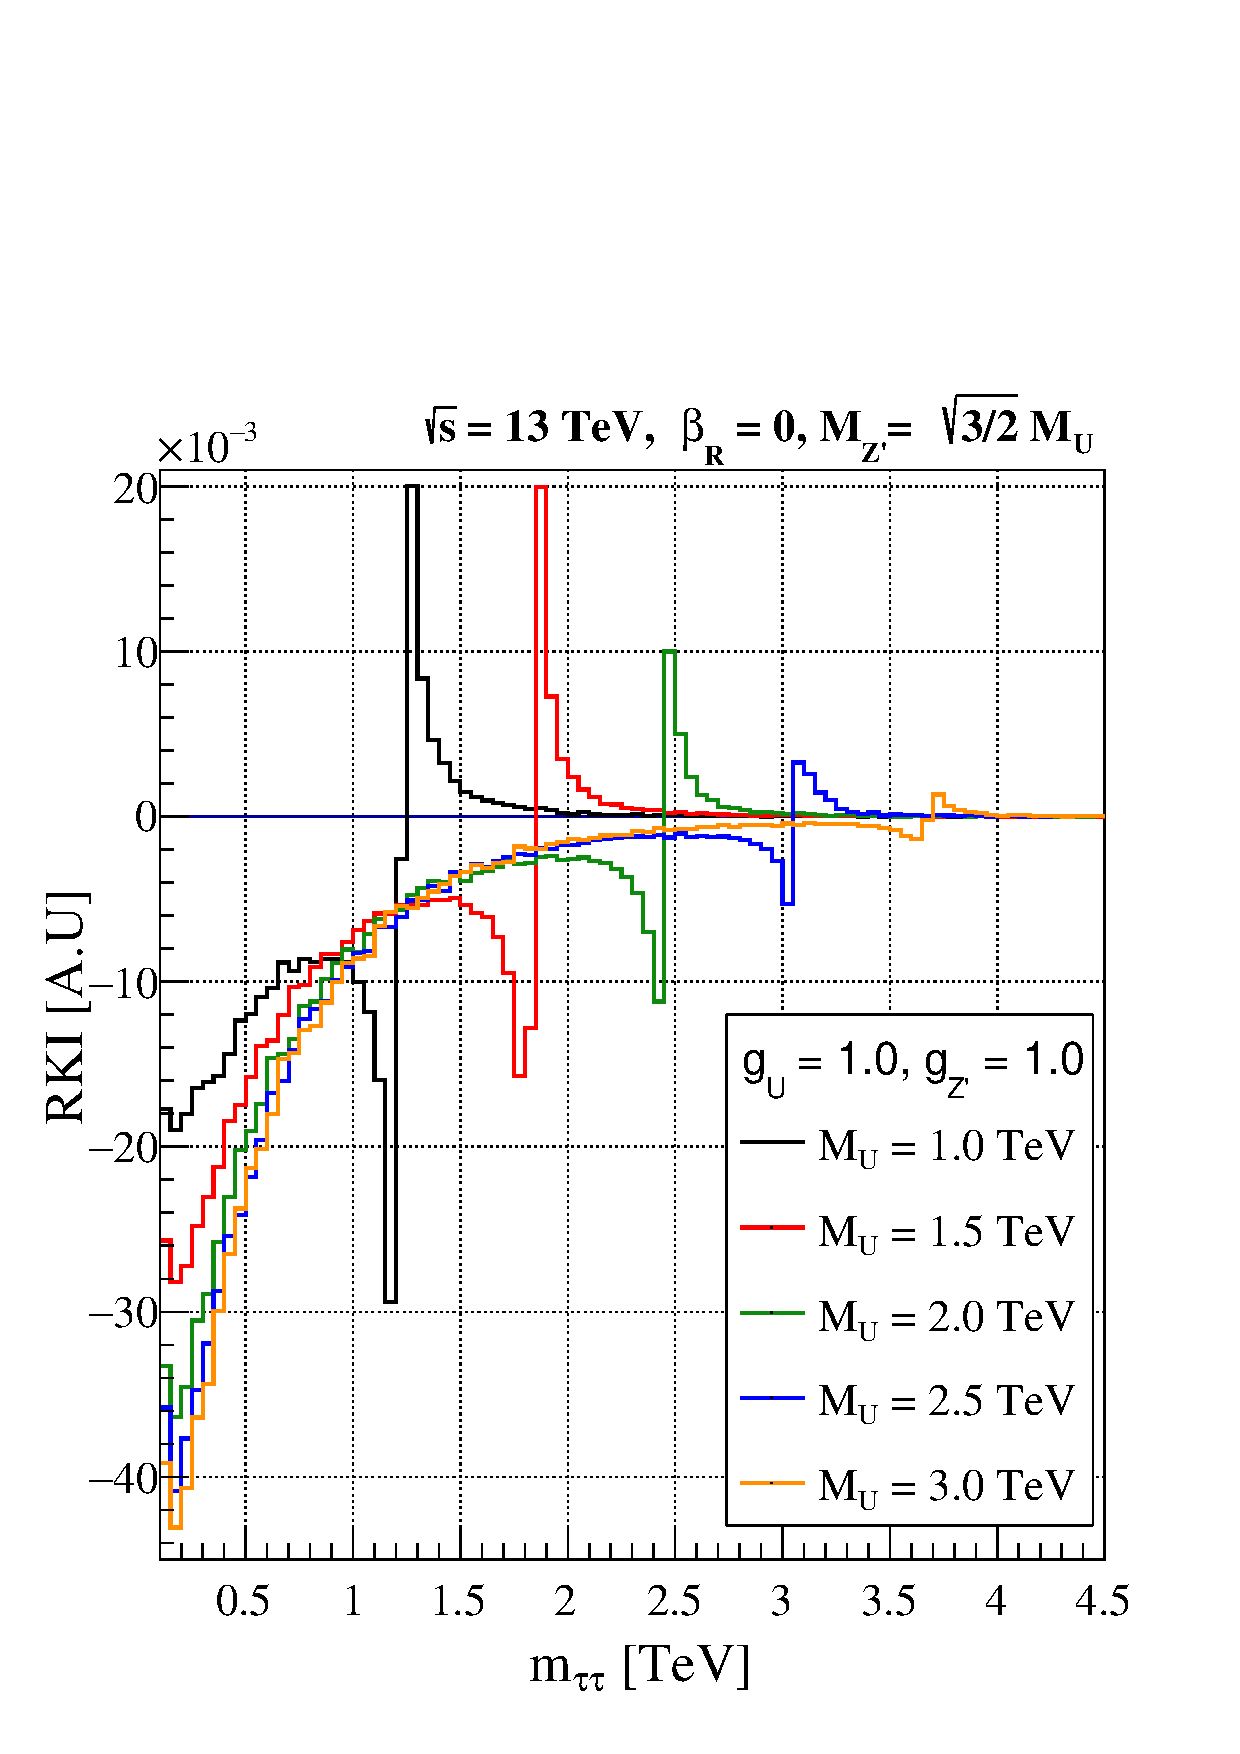
\includegraphics[width=.49\textwidth]{Images/Kinematic_Interference_gu_1.0_gzp_1.0_zp_upper_limit_woRHC.pdf}
    \captionof{figure}{The relative kinematic interference (RKI), as a function of the reconstructed mass of two taus, for different $\lq$ masses. The studies are performed assuming $\sqrt s=13 \tev$, $\beta_R=0$, $g_U = 1.0$, $g_{\zb^{\prime}} =1.0$, $M_{\zb^{\prime}} = \sqrt{1/2} M_{U}$ (left), and $M_{\zb^{\prime}} = \sqrt{3/2} M_{U}$ (right).
    }    
\label{fig:interference}
\end{center}
In order to further illustrate the effect, Fig.~\ref{fig:interference} shows the relative kinematic interference ($\mathrm{RKI}$) as a function of the reconstructed invariant mass $m_{\tau\tau}$, for $g_{\zb^{\prime}} = 1$ and varying values of $M_U$. The RKI parameter is defined as
\begin{equation}
    \mathrm{RKI}(m_{\tau\tau})=\frac{1}{\sigma_{\lq+\zb'}}\left[\frac{d\sigma_{\lq+\zb'}}{dm_{\tau\tau}}-\left(\frac{d\sigma_{\lq}}{dm_{\tau\tau}}+\frac{d\sigma_{\zb'}}{dm_{\tau\tau}}\right)\right],
\end{equation}
where $\sigma_{X}$ is the production cross-section arising due to contributions from $X$ particles. For example, $\sigma_{\lq+\zb'}$ represents the inclusive cross-section where both virtual $\lq$ and s-channel $\zb'$ exchange contribute. For both cases, we can observe the presence of deep valleys in the RKI curves when $m_{\tau\tau}\to0$, indicating destructive interference between the $\lq$ and the $\zb'$ contributions. This interference generates a suppression of the differential cross-section for lower values of $m_{\tau\tau}$ and, therefore, in the integrated cross-section. 
 
The observed interference effects are consistent with detailed studies on resonant and non-res $\mathrm{p}\,\mathrm{p}\to\tq \bar{\tq}$ production, performed in reference~\cite{Djouadi:2019cbm}.
\section{Search strategy and simulation}
\label{sec:strategyandsimulation}


Our proposed analysis strategy utilizes single-$\lq$ (i.e.\ $\mathrm{p}\,\mathrm{p}\to \tau\,\lq$), double-$\lq$ (i.e.\ $\mathrm{p}\,\mathrm{p}\to \lq\,\lq$), and non-resonant $\lq$ production (i.e.\ $\mathrm{p}\,\mathrm{p}\to \tau\tau$) as shown in Fig.~\ref{fig:feynmp-prod-channels}. At leading order in $\alpha_s$, since we focus on  $U_1\to \bq\,\tau$ decays, the s$\lq$ process results in the $\textrm{b}\tau\tau$ mode, the d$\lq$ process results in the $\textrm{bb}\tau\tau$ mode, and the non-res process results in the $\tau\tau$ mode. Therefore, in all cases we obtain two $\tau$ leptons, with either 0, 1, or 2 b jets. The $\tau$ leptons decay to hadrons ($\tau_{\textrm{h}}$) or semi-leptonically to electrons or muons ($\tau_{\ell}$, $\ell = \textrm{e}$ or $\mu$). To this end, we study six final states: $\tau_{\mathrm h} \tau_{\mathrm{h}/\ell}$, $\bq\,\tau_{\mathrm h} \tau_{\mathrm{h}/\ell}$, and $\bq \bq\,\tau_{\mathrm h} \tau_{\mathrm{h}/\ell}$, which can be naively associated to non-res, s$\lq$ and d$\lq$ production, respectively.
Nevertheless, experimentally it is possible for $\bq$ jets to not be properly identified or reconstructed, leading, for instance, to a fraction of d$\lq$ signal events falling into the $\bq\,\tau_{\mathrm h} \tau_{\mathrm{h}/\ell}$ and $\tau_{\mathrm h}\tau_{\mathrm{h}/\ell}$ categories. Similarly, soft jets can fake $\bq$ jets, such that non-res processes can contribute to the $\bq\,\tau_{\mathrm h} \tau_{\mathrm{h}/\ell}$ and $\bq\bq\,\tau_{\mathrm h} \tau_{\mathrm{h}/\ell}$ final states. This kind of signal loss and mixing is taken into account in our analysis\footnote{Note that further signal mixing can also occur at the event generation level by including terms at larger order in $\alpha_s$. For example, in the non-res diagram in Fig.~\ref{fig:feynmp-prod-channels}, one of the initial $\bq$ could come from a $g\to \bq\bar{\bq}$ splitting, leading to non resonant production of $\bq\,\tau_{\mathrm h} \tau_{\mathrm{h}/\ell}$. Simulating and studying the role of such NLO contributions is outside the scope of this work.}.

The contributions of signal and background events are estimated using Monte Carlo (MC) simulations. We implemented the $U_1$ model from~\cite{Baker:2019sli}, adjusted to describe the lagrangian in Equations~\eqref{eq:BasicLagrangian} and ~\eqref{eq:BasicLagrangianZp}, using \texttt{FeynRules} (v2.3.43) ~\cite{Christensen:2008py,Alloul:2013bka}. The branching ratios and cross-sections have been calculated using \texttt{MadGraph5\_aMC} (v3.1.0) \cite{Alwall:2014bza, Alwall:2014hca}, the latter at leading order in $\alpha_s$. The corresponding samples are generated considering $\mathrm{p}\,\mathrm{p}$ collisions at  $\sqrt{s}=13 \tev$ and $\sqrt{s}=13.6 \tev$.  All samples are generated using the NNPDF3.0 NLO~\cite{NNPDF:2014otw} set for parton distribution functions (PDFs) and using the full amplitude square SDE strategy for the phase-space optimization due to strong interference effects with the $\zb'$ boson. Parton level events are then interfaced with the \texttt{PYTHIA} (v8.2.44)~\cite{Sjostrand:2014zea} package to include parton fragmentation and hadronization processes, while \texttt{DELPHES} (v3.4.2)~\cite{deFavereau:2013fsa} is used to simulate detector effects, using the input card for the CMS detector geometric configurations, and for the performance of particle reconstruction and identification.

At parton level, jets and leptons are required to have a minimum transverse momentum ($\pt$) of $20 \gev$, while $\bq$ jets are required to have a minimum $\pt$ of $30 \gev$. Additionally, we constrain the pseudorapidity ($\eta$) to $|\eta| < 2.5$ for $\bq$ jets and leptons, and $|\eta| < 5.0$ for jets. The production cross-sections shown in the bottom panel of Figures~\ref{fig:branching_ratios} and~\ref{fig:xsinterference} are obtained with the aforementioned selection criteria. 

\begin{table}[t]
    \begin{tabular}{|c|cccccc|}
    \hline
    \multirow{2}{*}{\textbf{Variable}} & \multicolumn{6}{c|}{\textbf{Threshold}} \bigstrut\\ 
    \cline{2-7} 
                                      & \multicolumn{1}{c|}{$\tau_{h} \tau_{h}$} & \multicolumn{1}{c|}{$\bq \tau_{h} \tau_{h}$} & \multicolumn{1}{c|}{$\bq \bq \tau_{h} \tau_{h}$} & \multicolumn{1}{c|}{$\tau_{h} \tau_{\ell}$} & \multicolumn{1}{c|}{$\bq \tau_{h} \tau_{\ell}$} & $\bq \bq \tau_{h} \tau_{\ell}$ \bigstrut\\ \hline \hline


    $N(\bq)$                             & \multicolumn{1}{c|}{= 0} & \multicolumn{1}{c|}{= 1} & \multicolumn{1}{c|}{$\geq 2$} & \multicolumn{1}{c|}{= 0}& \multicolumn{1}{c|}{= 1} & $\geq 2$ \bigstrut\\ \hline
    $\pt(\bq)$                         & \multicolumn{1}{c|}{-} & \multicolumn{2}{c|}{$\geq 30 \gev$ } & \multicolumn{1}{c|}{-} & \multicolumn{2}{c|}{$\geq 30 \gev$ } \bigstrut\\ \hline
    $|\eta(\bq)|$                        & \multicolumn{1}{c|}{-} &\multicolumn{2}{c|}{$\leq 2.4$} & \multicolumn{1}{c|}{-} &\multicolumn{2}{c|}{$\leq 2.4$} \bigstrut\\ \hline
                                      
    $N (\ell)$                         & \multicolumn{3}{c|}{= 0}  & \multicolumn{3}{c|}{= 1} \bigstrut\\ \hline
    $\pt(\el)$                         & \multicolumn{3}{c|}{-} & \multicolumn{3}{c|}{$\geq 35 \gev$} \bigstrut\\ \hline
    $\pt(\mu)$                       & \multicolumn{3}{c|}{-} & \multicolumn{3}{c|}{$\geq 30 \gev$} \bigstrut\\ \hline
    $|\eta(\ell)|$                     & \multicolumn{3}{c|}{-} & \multicolumn{3}{c|}{$\leq 2.4$} \bigstrut\\ \hline

    $N(\tau_{h})$                      & \multicolumn{3}{c|}{ $= 2$} & \multicolumn{3}{c|}{= 1} \bigstrut\\ \hline
    $\pt(\tau_h)$                    & \multicolumn{6}{c|}{$\geq 50$ GeV} \bigstrut\\ \hline
    $|\eta(\tau_h)|$                   & \multicolumn{6}{c|}{$\leq 2.3$} \bigstrut\\ \hline
    $\Delta R(p_{i}, p_{j})$           & \multicolumn{6}{c|}{$\geq 0.3$} \bigstrut\\ \hline

    \end{tabular}

    \caption{Preliminary event selection criteria used to filter events before feeding them to the BDT algorithm. A $\Delta R(p_{i}, p_{j}) > 0.3$ requirement is imposed between all pairs of reconstructed particle candidates $p_{i}, p_{j}$. 
    }
    \label{table:selection_channels}
\end{table}
Tab.~\ref{table:selection_channels} shows the preliminary event selection criteria for each channel at analysis level. The channels are divided based on the multiplicity of $\bq$ jets, $N(\bq)$, number of light leptons, $N(\ell)$, number of hadronic tau leptons, $N(\tau_{\mathrm h})$, and kinematic criteria based on $\eta$, $\pt$ and spatial separation of particles in the detector volume $(\Delta R = \sqrt{(\Delta \eta)^{2} + (\Delta \phi)^{2}})$. The minimum $\pt$ thresholds for leptons are chosen  following references~\cite{CMS:2020wzx, CMS:2022goy, ATLAS:2021oiz}, based on experimental constrains associated to trigger performance. Following reference~\cite{CMS_BTV2016}, we use a flat identification efficiency for $\bq$ jets of 70\% across the entire $\pt$ spectrum with misidentification rate of 1\%. These values correspond with the  ``medium working point'' of the CMS algorithm to identify $\bq$ jets, known as DeepCSV. We also explored the ``Loose'' (``Tight'') working point using an efficiency of 85\% (45\%) and mis-identification rate of 10\% (0.1\%). The  ``medium working point'' was selected as it gives the best signal significance for the analysis. 

For the performance of $\tau_{\textrm{h}}$ identification in DELPHES, we consider the latest technique described in~\cite{CMS_DeepTau}, which is based on a deep neural network (i.e. DeepTau) that combines variables related to isolation and $\tau$-lepton lifetime as input to identify different $\tau_{\textrm{h}}$ decay modes. Following~\cite{CMS_DeepTau}, we consider three possible DeepTau ``working points'': (i) the ``Medium'' working point of the algorithm, which gives a 70\% $\tau_{\textrm{h}}$-tagging efficiency and 0.5\% light-quark and gluon jet mis-identification rate; (ii) the ``Tight'' working point, which gives a 60\% $\tau_{\textrm{h}}$-tagging efficiency and 0.2\% light-quark and gluon jet mis-identification rate; and (iii) the ``VTight'' working point, which gives a 50\% $\tau_{\textrm{h}}$-tagging efficiency and 0.1\% light-quark and gluon jet mis-identification rate. Similar to the choice of $\textrm{b}$-tagging working point, the choice of $\tau_{\textrm{h}}$-tagging working point is determined through an optimization process which maximizes discovery reach. The ``Medium'' working point was ultimately shown to provide the best sensitivity and therefore chosen for this study. For muons (electrons), the assumed identification efficiency is 95\% (85\%), with a 0.3\% (0.6\%) mis-identification rate~\cite{CMS-PAS-FTR-13-014,CMS_MUON_17001,CMS_EGM_17001}.

After applying the preliminary selection criteria, the primary sources of background are production of top quark pairs ($\tq\bar{ \tq}$), and single-top quark processes (single $\tq$), followed by production of vector bosons with associated jets from initial or final state radiation ($V$+jets), and pair production of vector bosons ($VV$). The number of simulated MC events used for each sample is shown in Tab.~\ref{table:MC_events}. 

\begin{table}[]
    \centering
    \begin{tabular}{|c|c|c|c|c|c|}
    \hline
    \textbf{Sample}               & $\tq \bar{\tq}$ & single $\tq$ & $VV$       & $V+$jets   & signals \bigstrut\\ \hline \hline
    \textbf{$\mathbf{N_{events}}\times 10^{-6}$} & 24.31      & 11.50   & 32.35 & 39.45 & 0.60 \bigstrut\\ \hline
    \end{tabular}
    \caption{The number of simulated events for the signal and background samples.}
    \label{table:MC_events}
\end{table}

We use two different sets of signal samples. The first set includes various $\set{M_{U},g_{U}}$ scenarios, for two different values of $\beta_R\in \set{0,-1}$. We generate signal samples for $M_{U}$ values between 250 GeV and 5000 GeV, in steps of 250 GeV. The considered $g_{U}$ coupling values are between 0.25 and 3.5, in steps of 0.25. Although the signal cross-sections depend on both $M_{U}$ and $g_{U}$, the efficiencies of our selections only depend on $M_{U}$ (for all practical purposes) since the decay widths are relatively small compared to the mass of $M_{U}$ ($\frac{\Gamma_{U}}{M_{U}} < 5$\%), and thus more sensitive to experimental resolution. In total there are 280 $\set{M_{U},g_{U},\beta_{R}}$ scenarios simulated for this first set of signal samples, and for each of these scenarios two subsets of samples are generated, which are used separately for the training and testing of the machine learning algorithm. The second set of signal samples is used to evaluate interference effects between $\lq$s and the $\zb^{\prime}$ bosons in non-res production. Using benchmark values $g_U=1.8$ and $\beta_R=0$, we consider various $\set{M_{U},g_{\zb^{\prime}}}$ scenarios for two different $\zb^{\prime}$ mass hypotheses, $\left(M_{\zb'}/M_U\right)^2 \in \Set{\tfrac{1}{2},\tfrac{3}{2}}$. The $M_{U}$ values vary between 500 GeV and 5000 GeV, in steps of 250 GeV. The $g_{\zb^{\prime}}$ coupling values are between 0.25 and 3.5, in steps of 0.25. Therefore, in total there are 280 $\set{M_{U},g_{\zb^{\prime}},\left(M_{\zb'}/M_U\right)^2}$ scenarios simulated for this second set of signal samples, and for each of these scenarios a total of $6.0 \times 10^{5}$ MC events are generated.


As noted previously, the simulated signal and background events are initially filtered using selections which are motivated by experimental constraints, such as the geometric constraints of the CMS detector, the typical kinematic thresholds for reconstruction of particle objects, and the available triggers. The remaining events after the preliminary event selection criteria are used to train and execute a BDT algorithm for each signal point in the $\set{M_{U},g_{U}}$ space, in order to maximize the probability to detect signal amongst background events. The BDT algorithm is implemented using the \texttt{scikit-learn}~\cite{pedregosa_scikit-learn_2011} and \texttt{xgboost} (XGB)~\cite{chen_xgboost_2016} python libraries. We use the the \texttt{XGBClassifier} class from the \texttt{xgboost} library, a 10-fold cross validation using the \texttt{scikit-learn} method (\texttt{GridCV}  \footnote{GridCV is a method that allows to find the best combination of hyperparameter values for the model, as this choice is crucial to achieve an optimal performance.}) for a grid in a hyperparameter space with 75, 125, 250, and 500 estimators, maximum depth in 3, 5, 7, 9, as well as learning rates of 0.01, 0.1, 1, and 10. For the cost function, we utilize the default mean square error (\texttt{MSE}). Additionally, we use the tree method based on the approximate greedy algorithm (histogram-optimized), referred to as \texttt{hist}, with a uniform sample method. These choices allow us to maximize the detection capability of the BDT algorithm by carefully tuning the hyperparameters, selecting an appropriate cost function, and utilizing an optimized tree construction method.  


For each of the six analysis channels and $\set{M_{U},g_{U}}$ signal point, the binary XGB classifier was trained (tested) with 20\% (80\%) of the simulated events, for each signal and background MC sample. 
%, under the narrow width approximation. 
Over forty kinematic and topological variables were studied as input for the XGB. These included the momenta of b jets and $\tau_{\textrm{h},\ell}$ candidates; both invariant and transverse masses of pairs of $\tau$ objects and of $\textrm{b}\,\tau$ combinations; angular differences between b jets, between $\tau$ objects, and between the $\tau_{\textrm{h},\ell}$ and b jets; and additional variables derived from the missing momentum in the events. After studying correlations between variables and their impact on the performance of the BDT, we found that only eight variables were necessary and responsible for the majority of the sensitivity of the analysis.  
The variable that provides the best signal to background separation is the scalar sum of the $\pt$ of the final state objects ($\tau_{\mathrm h}$, $\tau_{h/\ell}$, and $\bq$ jets) and the missing transverse momentum, referred to as $S_{\mathrm{T}}^{MET}$: 
\begin{equation}
S_{\mathrm{T}}^{MET}=|\vec{p}_T^{\;miss}|+\sum_{\tau_{\mathrm h},\,\tau_{h/\ell},\,\bq}|\vec{p}_T|
\end{equation}
The $S_{\mathrm{T}}^{MET}$ variable has been successfully used in $\lq$ searches at the LHC, since it probes the mass scale of resonant particles involved in the production processes. Other relevant variables include the magnitude of the vectorial difference in $\pt$ between the two lepton candidates ($|\Delta \vec{p}_T |_{\tau_{\textrm{h}} \tau_{\textrm{h}/\ell}}$), the $\Delta R_{\tau_{\textrm{h}} \tau_{\textrm{h}/\ell}}$ separation between them, the reconstructed dilepton mass $m_{\tau_{\textrm{h}}\tau_{\textrm{h}/\ell}}$, and the product of their electric charges ($Q_{\tau_{\textrm{h}}} \times Q_{\tau_{\textrm{h}/\ell}}$). 
We also use the $|\Delta \vec{p}_T|$ between the $\tau_{\mathrm h}$ candidate and $\vec{p}_T^{\,miss}$, and (if applicable) the $|\Delta \vec{p}_T|$ between the $\tau_{\textrm{h}}$ candidate and the leading $\bq$ jet. For the final states including two $\tau_{\textrm{h}}$ candidates, the one with the highest $\pt$ is used. 

\begin{center}
    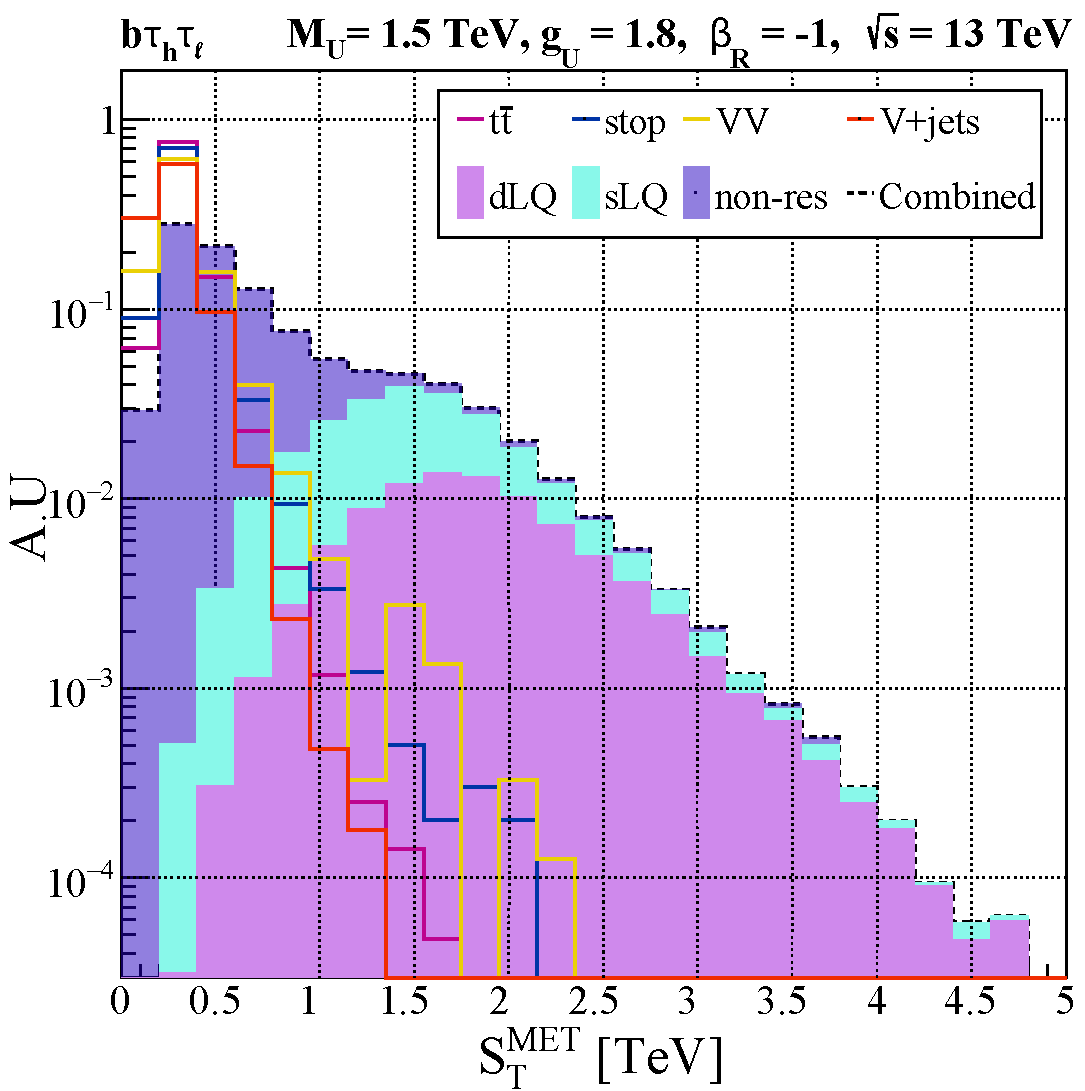
\includegraphics[width=.45\textwidth]{Images/Kinematic_Histograms/sTTeV_semileptonic_sLQ_wRHC.pdf}
    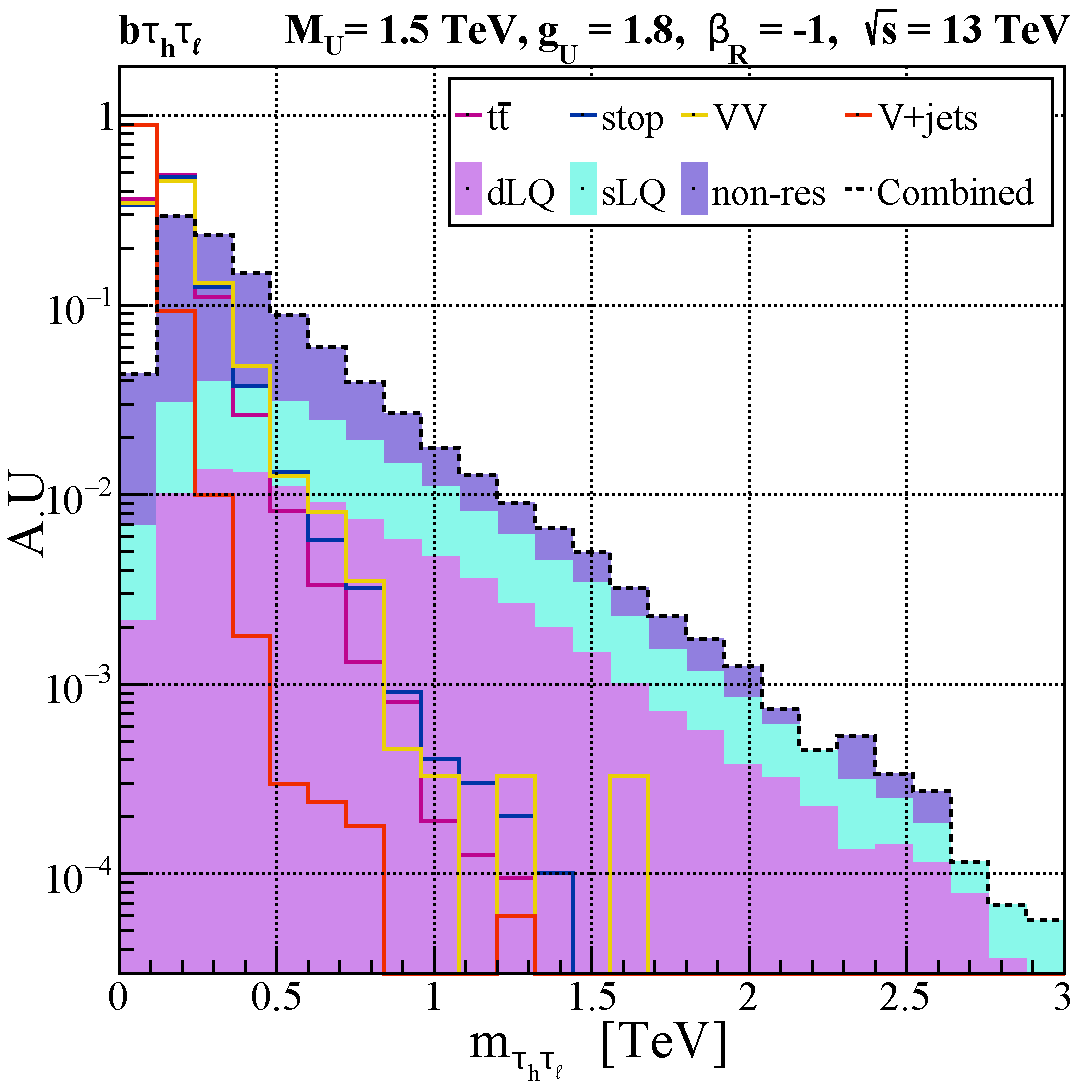
\includegraphics[width=.45\textwidth]{Images/Kinematic_Histograms/mTeV_semileptonic_sLQ_wRHC.pdf}
    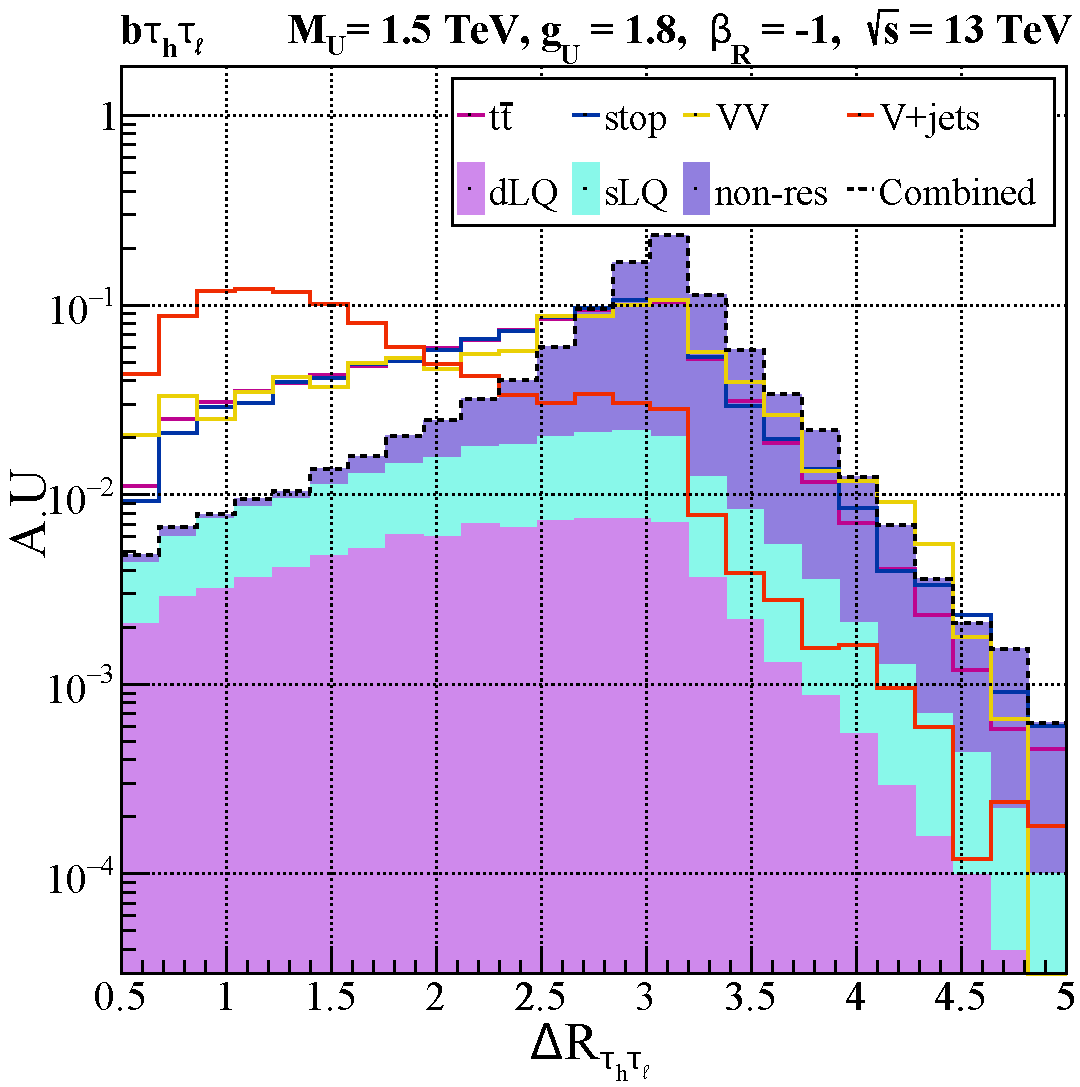
\includegraphics[width=.45\textwidth]{Images/Kinematic_Histograms/DeltaR_semileptonic_sLQ_wRHC.pdf}
    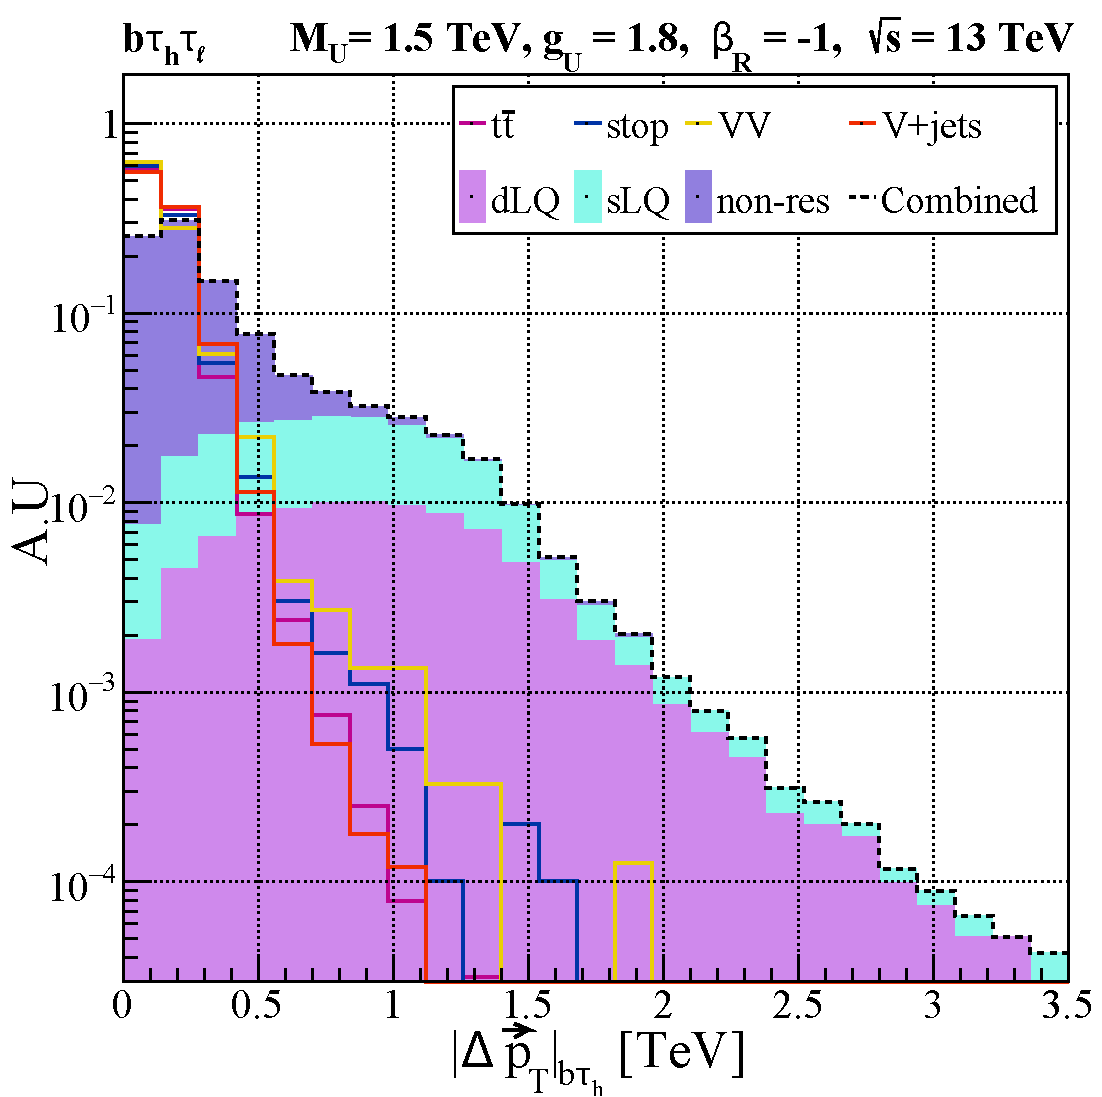
\includegraphics[width=.45\textwidth]{Images/Kinematic_Histograms/DeltaVecPT_semileptonic_sLQ_wRHC.pdf}    
    \captionof{figure}{$S_{\mathrm{T}}^{MET}$, $m_{\tau_{\mathrm h} \tau_{\ell}}$, $\Delta R_{\tau_{\mathrm h}\tau_{\ell}}$, $|\Delta \vec{p}_T|_{b \tau_{\mathrm h}}$ signal and background distributions for the $b\tau_h\tau_\ell$ channel. The signal distributions are generated for a benchmark sample with $\lq$ mass of $1.5 \tev$  maximally coupled to right-handed currents. The combined distribution (shown as a stacked histogram) is the sum of the distributions, correctly weighted according to their respective cross-sections, assuming a coupling $g_U = 1.8$.}
    \label{fig:sT(TeV)_wRHC}
\end{center}




Fig.~\ref{fig:sT(TeV)_wRHC} shows some relevant topological distributions, including $S_{\mathrm{T}}^{MET}$ on the top, for the $\bq\, \tau_{\mathrm h} \tau_{\ell}$ category.  
In the Figure we include all signal production modes to this channel, with each component weighted with respect to their total contribution to the combined signal. The combined signal distribution is normalised to unity. We also show all background processes contributing to this channel, each of them individually normalised to unity. We find that the combined signal is dominated by s$\lq$ production for large values of $S_{\mathrm{T}}^{MET}$, while non-res production dominates for small $S_{\mathrm{T}}^{MET}$. Interestingly, the backgrounds also sit at low $S_{\mathrm{T}}^{MET}$ values, since $S_{\mathrm{T}}^{MET}$ is driven by the mass scale of the SM particles being produced, in this case top quarks and Z/W bosons. This suggest that the s$\lq$ and d$\lq$ signals can indeed be separated from the SM background. As expected, the $S_{\mathrm{T}}^{MET}$ s$\lq$ and d$\lq$ signal distributions have a mean near $M_U$, representative of resonant production, and a broad width as expected for large mass $M_{U}$ hypotheses when information about the $z$-components of the momenta of objects is not utilised in the $S_{\mathrm{T}}^{MET}$ calculation.  

Fig.~\ref{fig:sT(TeV)_wRHC} (second from the top) shows the reconstructed mass of the ditau system, for the $\bq \tau_{\textrm{h}}\tau_{\ell}$ search channel. Since the two $\tau$ candidates in signal events arise from different production vertices (e.g., each $\tau$ candidate in d$\lq$ production comes from a different $\lq$ decay chain), the ditau mass distribution for signal scales as $m_{\tau_{\textrm{h}}\tau_{\ell}} \sim \pt(\tau_{\textrm{h}}) + \pt(\tau_{\ell})$, and thus has a tail which depends on $M_{U}$ and sits above the expected SM spectrum. On the other hand, the SM $m_{\tau_{\textrm{h}}\tau_{\ell}}$ distributions sit near $m_{\textrm{Z/W}}$ since the $\tau$ candidates in SM events arise from $\zb/\wb$ decays.

Fig.~\ref{fig:sT(TeV)_wRHC} (third from the top) shows the $\Delta R_{\tau_{\textrm{h}}\tau_{\ell}}$ distribution for the $\textrm{b}\tau_{\textrm{h}}\tau_{\ell}$ channel. In the case of the $\mathrm{p}\,\mathrm{p}\to\tau\tau$ non-res signal distribution, the two $\tau$ leptons must be back-to-back to preserve conservation of momentum. Therefore, the visible $\tau$ candidates, $\tau_{\textrm{h}}$ and $\tau_{\ell}$, give rise to a $\Delta R_{\tau_{\textrm{h}}\tau_{\ell}}$ distribution that peaks near $\pi$ radians. In the case of s$\lq$ production, although the $\lq$ and associated $\tau$ candidate must be back-to-back, the second $\tau$ candidate arising directly from the decay of the $\lq$ does not necessarily move along the direction of the $\lq$ (since the $\lq$ also decays to a b quark). As a result, the $\Delta R_{\tau_{\textrm{h}}\tau_{\ell}}$ distribution for the s$\lq$ signal process is smeared out, is broader, and has a mean below $\pi$ radians. On the other hand, the $\tau_{\textrm{h}}$ candidate in $\tq\bar{ \tq}$ events is often a jet being misidentified as a genuine $\tau_{\textrm{h}}$. When this occurs, the fake $\tau_{\textrm{h}}$ candidate can arise from the same top quark decay chain as the $\tau_{\ell}$ candidate, thus giving rise to small $\Delta R_{\tau_{\textrm{h}}\tau_{\ell}}$ values. This difference in the signal and background distributions provides a nice way for the ML algorithm to help decipher signal and background processes.

As noted above, the $|\Delta \vec{p}_{T}|$ distribution between the visible $\tau$ candidates and the b-quark jets is an important variable to help the BDT distinguish between signal and background processes. The discriminating power can be seen in Fig.~\ref{fig:sT(TeV)_wRHC} (bottom), which shows the $|\Delta \vec{p}_{T}|$ between the $\tau_{\textrm{h}}$ and b-jet candidate of the $\textrm{b}\tau_{\textrm{h}}\tau_{\ell}$ channel. In the case of d$\lq$ production, the b quarks and $\tau$ leptons from the $\lq \to \textrm{b}\tau$ decay acquire transverse momentum of $p_{T} \sim M_{U}/2$. However, when the $\tau$ lepton decays hadronically (i.e. $\tau \to \tau_{\textrm{h}}\nu$), a large fraction of the momentum is lost to the neutrino. Therefore, the $|\Delta \vec{p}_{T}|_{\textrm{b}\tau_{\textrm{h}}}$ distribution for the d$\lq$ (and s$\lq$) process peaks below $M_{U}$/2. On the other hand, for a background process such as V+jets, the b jet arises due to initial state radiation, and thus must balance the momentum of the associated vector boson (i.e. $p_{T}(\textrm{b}) \sim p_{T}(\textrm{V}) \sim m_{\textrm{V}}$). Since the visible $\tau$ candidate is tyically produced from the V boson decay chain, its momentum (on average) is approximately $p_{T}(\tau_{\textrm{h}}) \sim p_{T}(\textrm{V})/4 \sim m_{\textrm{V}}/4$. Therefore, to first order, the $|\Delta \vec{p}_{T}|$ distribution for the V+jets background is expected to peak below the $m_{\textrm{V}}$ mass. 

\begin{figure}[]
    \centering
    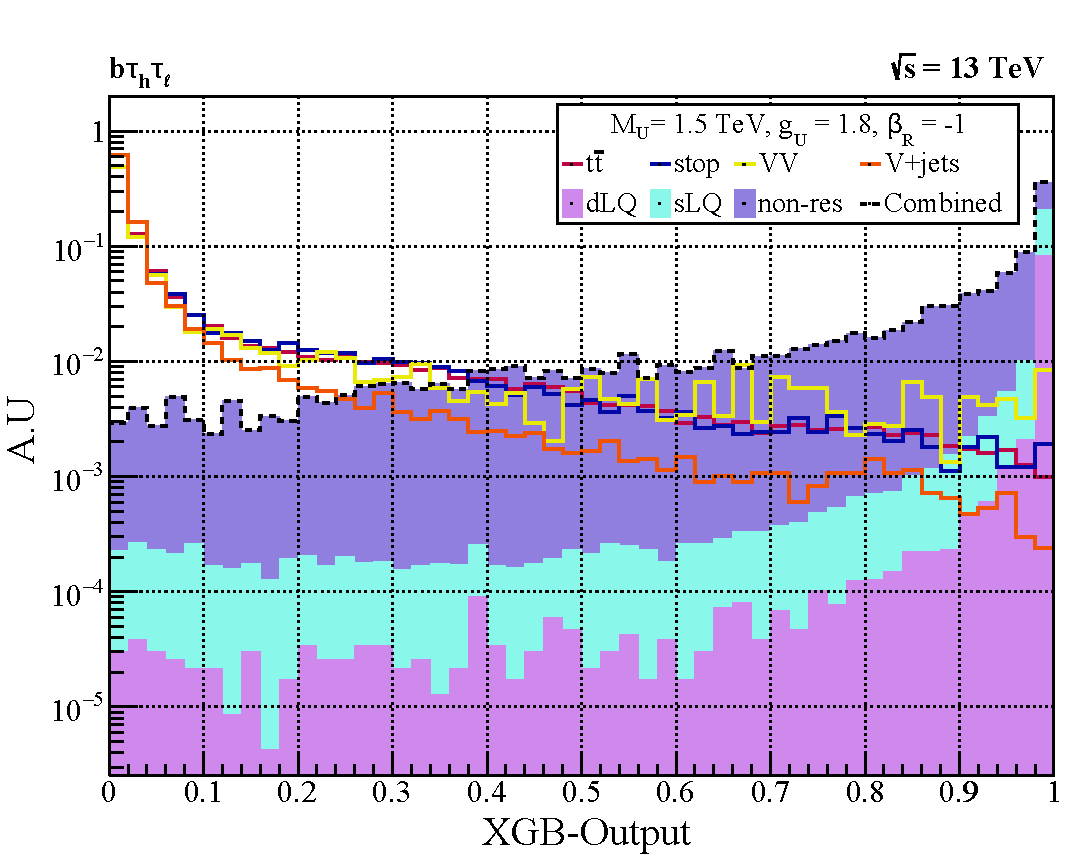
\includegraphics[width=.75\linewidth]{Images/ML_semileptonic_sLQ_wRHC.pdf}
    \caption{Postfit XGB-output normalised distribution in the $\bq\, \tau_{\mathrm h} \tau_{\ell}$ channel, for $\lq$ mass of 1.5\tev, constant coupling $g_U=1.8$, and maximally coupled to right-handed currents.}
    \label{fig:XGB_output}
\end{figure}
Lets us turn to the results of the $\bq\tau_{\mathrm h}\tau_\ell$ BDT classifier, which is shown in Fig.~\ref{fig:XGB_output} for the different signal production modes and backgrounds. Similar to Fig.~\ref{fig:sT(TeV)_wRHC}, the distribution for each individual signal production mode is weighted with respect to their total contribution to the combined signal. The background distributions and combined signal distribution are normalized to an area under the curve of unity. Fig.~\ref{fig:XGB_output} shows the XGB distributions for a signal benchmark point with $M_{U} = 1.5$ TeV, $g_{U} = 1.8$, and $\beta_{R} = -1$. The XGB output is a value between 0 and 1, which quantifies the likelihood that an event is either signal-like (XGB output near 1) or background-like (XGB output near 0). We see that the presence of the s$\lq$ and d$\lq$ production modes is observed as an enhancement near a XGB output of unity, while the backgrounds dominate over the low end of the XGB output spectrum, especially near zero. In fact, over eighty percent of the sLQ and dLQ distributions reside in the last two bins, XGB output greater than 0.96, while more than sixty percent of the backgrounds fall in the first two bins, XGB output less than 0.04. %\JPP{23\% lie on the left of XGB = 0.7}.
It is also interesting to note that in comparison to the sLQ and dLQ distributions in Fig.~\ref{fig:XGB_output}, non-res is broader and not as narrowly peaked near XGB output of 1, which is expected due to the differences in kinematics described above. Overall, if we focus on the last bin in this distribution, we find approximately 0.2\% of the background, in contrast to 22\% of the non-res, 78\% of the sLQ, and 91\% of the dLQ signal distributions. These numbers highlight the effectiveness of the XGB output in reducing the background in the region where the signal is expected.

The output signal and background distributions of the XGB classifier, normalised to their cross section times pre-selection efficiency times luminosity, are used to perform a profile binned likelihood statistical test in order to determine the expected signal significance. The estimation is performed using the \texttt{RooFit}~\cite{RooFit} package, following the same methodology as in Refs.~\cite{Barbosa:2022mmw, Florez:2021zoo, Florez:2019tqr, Florez:2018ojp, Florez:2017xhf, VBFZprimePaper, Florez:2016lwi, U1T3R, mSUGRApaper, SupercriticalString, ConnectingPPandCosmology, VBF1, DMmodels2, VBFSlepton, VBFStop, VBFSbottom}. The value of the significance ($Z_{sig}$) is measured using the probability to obtain the same outcome from the test statistic in the background-only hypothesis, with respect to the signal plus background hypothesis. This allows for the determination of the local p-value and thus the calculation of the signal significance, which corresponds to the point where the integral of a Gaussian distribution between $Z_{sig}$ and $\infty$ results in a value equal to the local p-value. 

Systematic uncertainties are incorporated as nuisance parameters, considering log-priors for normalization and Gaussian priors for shape uncertainties. Our consideration of systematic uncertainties includes both experimental and theoretical effects, focusing on the dominant sources of uncertainty. Following~\cite{lumiRef}, we consider a 3\% systematic uncertainty on the measurement of the integrated luminosity at the LHC. A 5\% uncertainty arises due to the choice of the parton distribution function used for the MC production, following the PDF4LHC prescription~\cite{Butterworth:2015oua}. The chosen PDF set only has an effect on the overall expected signal and background yields, but the effect on the shape of the XGB output distribution is negligible. Reference~\cite{CMS_DeepTau} reports a systematic uncertainty of 2-5\%, depending on the $p_{\textrm{T}}$ and $\eta$ of the $\tau_{\textrm{h}}$ candidate. Therefore, we utilize a conservative 5\% uncertainty per $\tau_{\textrm{h}}$ candidate, independent of $p_{\textrm{T}}$ and $\eta$, which is correlated between signal and background processes with genuine $\tau_{\textrm{h}}$ candidates, and correlated across XGB bins for each process. We assumed a 5\% $\tau_{\textrm{h}}$ energy scale uncertainty, independent of $p_{\textrm{T}}$ and $\eta$, following the CMS measurements described in~\cite{CMS_DeepTau}.  Finally, we assume a conservative 3\% uncertainty per b-jet candidate, following reference~\cite{CMSbtag}, and an additional 10\% uncertainty in all the background predictions to account for possible mismodeling by the simulated samples. The uncertainties on the background estimates are typically derived from collision data using dedicated control samples that have negligible signal contamination and are enriched with events from the specific targeted background. The systematic uncertainties on the background estimates are treated as uncorrelated between background processes.
\begin{figure}[]
    \centering
        \begin{subfigure}[b]{.48\linewidth}
            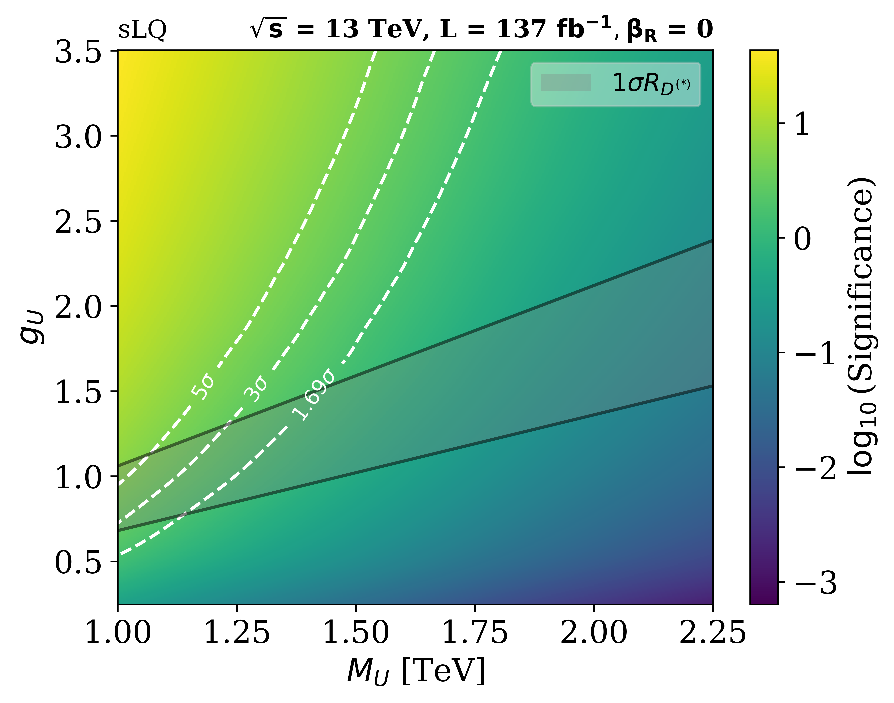
\includegraphics[width=\linewidth]{Images/Significance/Significance_Heatmap_13TeV_L137_sLQ_combined_woRHC.pdf}
        \end{subfigure}
        \begin{subfigure}[b]{.48\linewidth}
            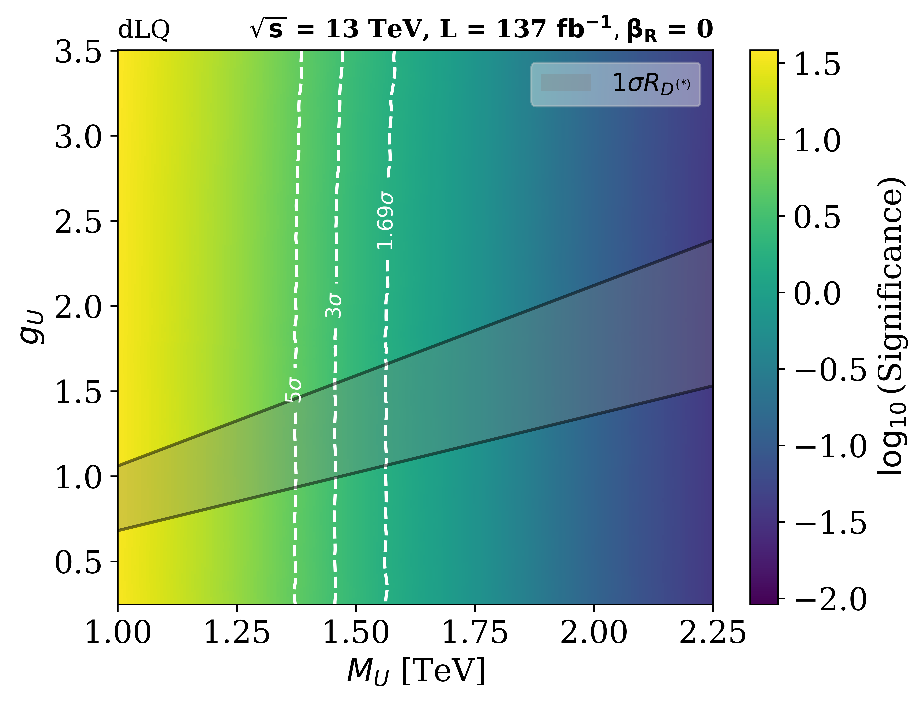
\includegraphics[width=\linewidth]{Images/Significance/Significance_Heatmap_13TeV_L137_dLQ_combined_woRHC.pdf}
        \end{subfigure}     
        \begin{subfigure}[b]{.48\linewidth}
            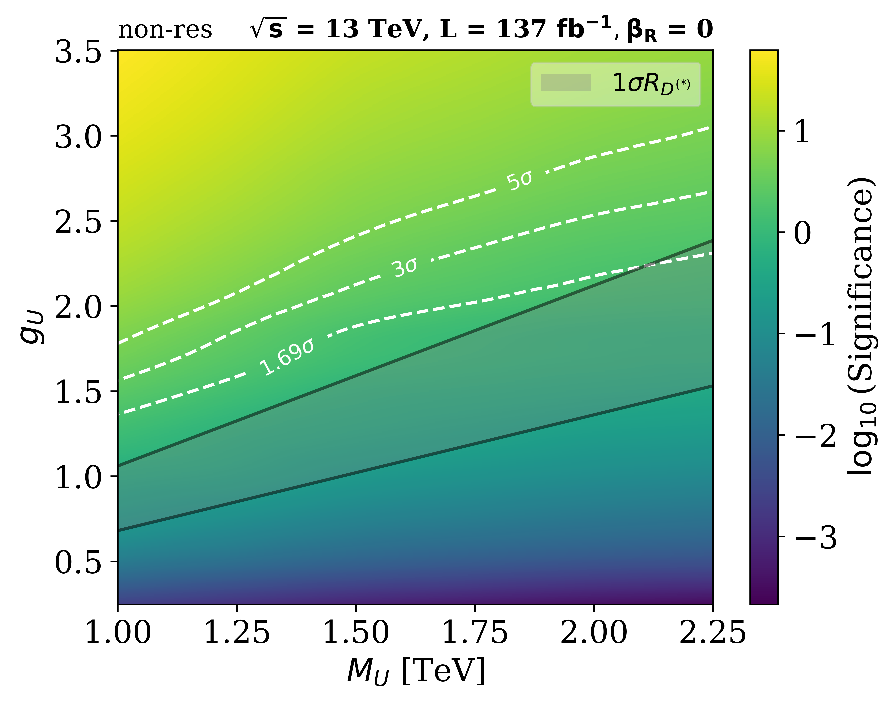
\includegraphics[width=\linewidth]{Images/Significance/Significance_Heatmap_13TeV_L137_non-res_combined_woRHC.pdf}
        \end{subfigure}    
 
    \caption{Signal significance for different coupling scenarios and $\lq$ masses, without right-handed currents, using the combination of all search channels. The results pertaining to  s$\lq$, d$\lq$ and non-res production are displayed respectively from the top.  These results are for $\sqrt{s} = 13 \tev$ and $137 \fb^{-1}$.}
    \label{fig:heatmapssignificance}
\end{figure}

\section{Samples and Simulation}\label{sec:sims}

\begin{center}
  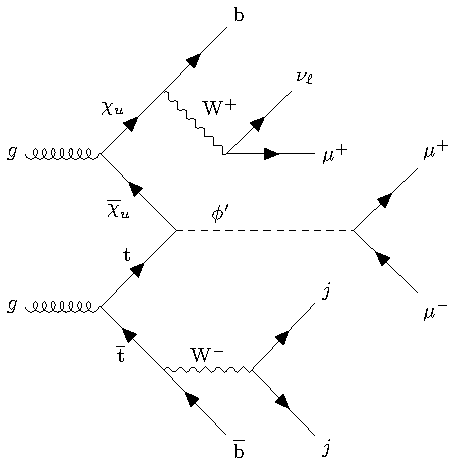
\includegraphics[width=0.75\linewidth]{Images/signal_qqfusion.pdf}
    \captionof{figure}{Representative Feynman diagram for the production of a $\phi'$ boson in association with a $\chi_\mathrm{u}$ vector-like quark through the fusion of a top quark and $\chi_\mathrm{u}$ vector-like quark. Once again, the $\phi'$ decays to a pair of muons, the top quark decays fully hadronically, and the $\chi_\mathrm{u}$ decays semi-leptonically to muons, neutrinos and $b$-jets.\label{fig:qqfusion}}
\end{center}

\begin{center}
    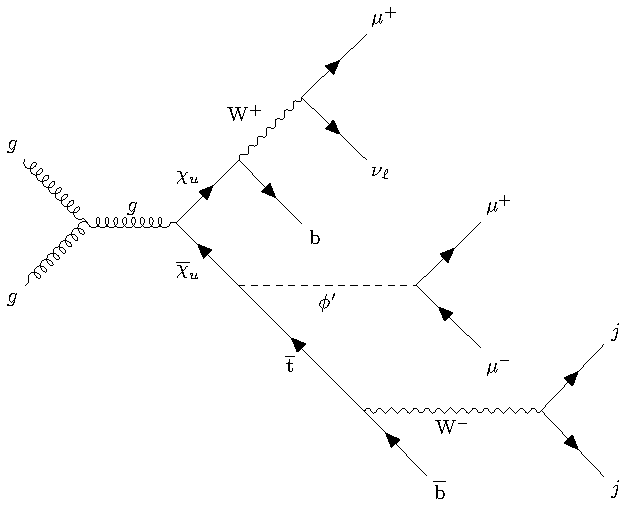
\includegraphics[width=0.85\linewidth]{Images/signal_ggfusion.pdf}
    \captionof{figure}{Representative Feynman diagram for the production of a $\phi'$ boson in association with a $\chi_\mathrm{u}$ vector-like quark through the fusion of a gluon pair from incoming protons. The $\phi'$ decays to a pair of muons, the top quark that decays fully hadronically, and the $\chi_\mathrm{u}$ decay semi-leptonically to muons, neutrinos and jets.\label{fig:ggfusion}}
\end{center}

The minimal $U(1)_{T^3_R}$ model described in Sec.~\ref{sec:model} is implemented \textit{at tree level} into the \texttt{FeynRules} package~\parencite{Alloul:2013bka}, which generates the Feynman rules and exports them into a Universal \texttt{FeynRules} Output (\texttt{UFO})~\parencite{Degrande:2011ua}. The resulting \texttt{UFO} is utilized as input for a generator to produce the MC samples. Both signal and background events are generated with the \texttt{MadGraph5\_aMC@NLO} v3.2.0 program~\parencite{Alwall:2014hca,Alwall:2014bza} at leading order (LO) in QCD, considering \textrm{pp} beams colliding with a center-of-mass energy of $\sqrt{s} = 13.6$ \textrm{TeV}. Each signal and background sample is generated separately, with no interference effects between the signal and background considered. The impact of these interference effects has been evaluated, and for all values of $\chi_\mathrm{u}$ and $\phi'$ masses considered, the effect on the signal plus background cross section is found to be less than $<0.5$\%. Additionally, the effect on the shape of the b-jet $p_{T}$ distribution is less than 6\% for $p_{T} < 300$ GeV and less than 2\% for b-jet $p_{T} > 300$ GeV. We use the \texttt{NNPDF3.0~NLO}~\parencite{NNPDF:2014otw} set for parton distribution functions (PDFs) for all event generation. Parton-level events are then interfaced with \texttt{PYTHIA} (v8.2.44)~\parencite{Sjostrand:2014zea} to account for parton showering and hadronization processes. Finally, we use  \texttt{DELPHES} (v3.4.2)~\parencite{deFavereau:2013fsa} to simulate smearing and other detector effects using the CMS detector geometric configurations and parameters for particle identification and reconstruction, using the CMS input card with 140 average pileup interactions. All signal cross sections used in this analysis are obtained requiring the following kinematic criteria on leptons $\ell$, \textrm{b} quarks, and light-quark/gluon jets ($j$) at parton level in \texttt{MadGraph}: $p_{\mathrm{T}}(\ell) > 35$~\textrm{GeV}, $\abs{\eta (\mathrm{b})} < 2.5$, $\abs{\eta (\ell)} < 2.3$, $p_{\mathrm{T}}(j) > 20$~\textrm{GeV}, and $\abs{\eta (\mathrm{j})} < 5$. These parton-level selections were applied exclusively to the signal processes to restrict event generation to the relevant phase space regions. For background processes, these default parton level requirements in \texttt{MadGraph} were imposed:  $p_{\mathrm{T}}(\ell) > 10$~\textrm{GeV}, $\abs{\eta (\ell)} < 2.5$, $p_{\mathrm{T}}(j) > 20$~\textrm{GeV}, $\abs{\eta (\mathrm{j})} < 5$, and $\abs{\eta (\mathrm{b})} < 5$. This ensures that the phase space regions for the background near the analysis-level selection criteria are adequately described after parton showering since the pre-selections at the analysis level are more stringent than the parton-level requirements. Furthermore, we use the MLM algorithm for jet matching and jet merging. The parameters \texttt{xqcut} and \texttt{qcut} of the MLM algorithm are set to 30 and 45 respectively to ensure continuity of the differential jet rate as a function of jet multiplicity. Each simulated signal and background sample is produced separately at LO, with one million events at the generation level, neglecting potential interference effects between the signal and background due to the suppression caused by the different orders of magnitude in the coupling constants of the signal and background.

Signal samples are generated considering the production of a $\phi'$ boson, an associated $\chi_\mathrm{u}$ vector-like quark, and a top quark $(\mathrm{pp}\to \chi_\mathrm{u} \mathrm{t} \phi')$, inclusive in both $\alpha$ and $\alpha_s$ (see Figures~\ref{fig:qqfusion}-\ref{fig:ggfusion}). We have used the implementation of the $U(1)_{T^3_R}$ model in Ref.~\parencite{Dutta2023}. Signal samples were created considering coupling values of $Y_{\mathrm{t}_R}=Y_{\mathrm{t}_L}=2\sqrt{2}$ in the range of masses $m(\phi')\in\{5,10,50,100,325\}$~\textrm{GeV} for the dark higgs and $m(\chi_\mathrm{u})\in\{0.50, 0.75, 1.0, 1.5, 2.0, $ $ 2.5\}$~\textrm{TeV} for the vector-like quark $\chi_u$~\parencite{PhysRevD.108.095006}. The production cross section for $\mathrm{pp}\to \chi_\mathrm{u} \mathrm{t} \phi'$ is highly dependent on the choice of the Yukawa couplings in the Lagrangian. The ${\chi_\mathrm{u}}{- \mathrm{t}}$ fusion process shown in Figure~\ref{fig:qqfusion} is dominated by the $Y_{\mathrm{t}_R}$ coupling. However, the decay ${\chi_\mathrm{u}} \to \mathrm{t} \phi'$ shown in Figure~\ref{fig:ggfusion} is inversely proportional to the $Y_{\mathrm{t}_L}$ coupling. This effect is shown in Figure~\ref{fig:cross_section_by_lambdas}, which displays the total signal cross section, as a function of $Y_{\mathrm{t}_R}$ and $Y_{\mathrm{t}_L}$, for a benchmark point with $m(\phi')=100$~\textrm{GeV} and $m(\chi_\mathrm{u})=1.0$~\textrm{TeV}. 

\begin{figure}
    \centering
    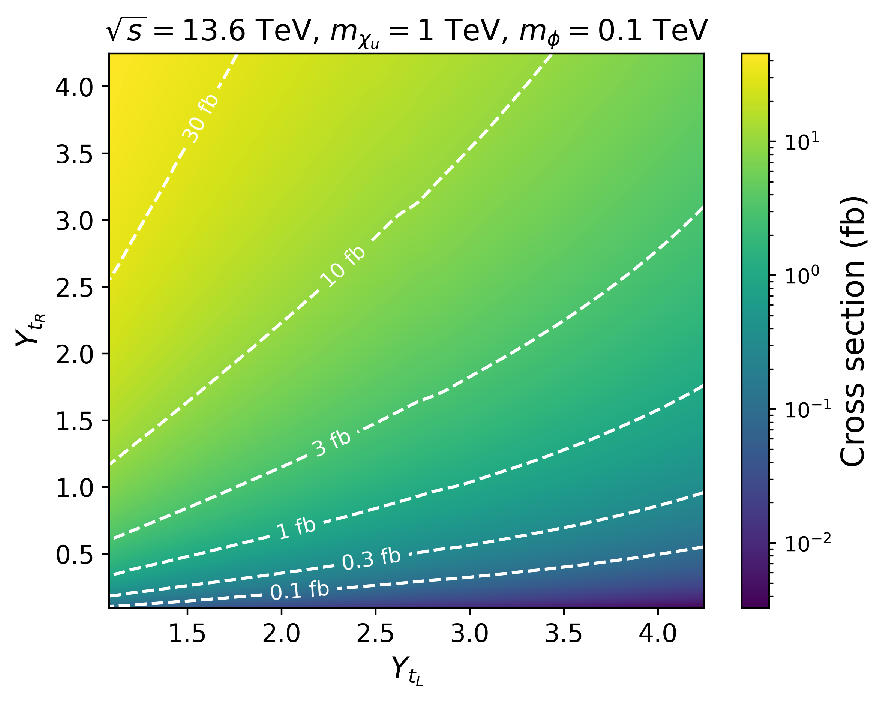
\includegraphics[width=0.85\linewidth]{Images/cross_section_by_lambdas.pdf}
    \caption{Signal production cross section, $ \mathrm{pp}\to \chi_\mathrm{u} \mathrm{t} \phi'$,  in the $Y_{\mathrm{t}_R}$ versus $Y_{\mathrm{t}_L}$ plane, for a benchmark point with $m(\phi')=100$~\textrm{GeV} and $m(\chi_\mathrm{u})=1.00$~\textrm{TeV}. The white-dashed contours show specific cross section values in the two dimensional plane.}
    \label{fig:cross_section_by_lambdas}
\end{figure}

We target signal events where the top quark decays hadronically into a bottom quark and two jets ($\mathrm{t} \to \mathrm{bW} \to \mathrm{b} q \bar{q}'$), the $\chi_\mathrm{u}$ decays semileptonically into a $b$ quark, lepton, and neutrino (via $\chi_\mathrm{u} \to \mathrm{bW}$ and $\mathrm{W}\to\mu\nu_{\mu}$), and the $\phi'$ produces two muons. We note that the scalar $\phi'$ particle could result from the mixture of the SM Higgs boson and additional scalar fields, and the Yukawas of the fermions could additionally arise from the mixing of the SM fermions with additional copies of the associated vector-like fermions. Therefore, the $\phi'$ branching ratios are dependent on the chosen mechanism and model by which this mixture occurs, see for example, Refs.~\parencite{Cacciapaglia_2023,Blankenburg:2012nx,Jones-Perez:2013oia,Calibbi:2009pv}. For the purpose of this work, and 
similar to Refs.~\parencite{Dutta2020,Dutta2023}, the considered benchmark signal scenarios have $\mathfrak{B}(\chi_\mathrm{u} \rightarrow \textrm{b W})$ of about 0.5 and $\mathfrak{B}(\phi' \rightarrow \mu^+\mu^-)=1.00$. Figure~\ref{fig:xs-plot} shows the production cross section in \textrm{fb}, as a function of $m(\phi')$ and $m(\chi_\mathrm{u})$ masses, assuming the aforementioned decays, branching ratios, and couplings.

We note that for the parameter space of focus in this paper, the total mass of the $t$-$\chi_\mathrm{u}$ system is larger than $m(\phi')$, thus the large rest energy of the $t$-$\chi_\mathrm{u}$ system is converted into potentially large momentum values for the $\phi'$. Similarly, the $t$-quark produced through the $\chi_\mathrm{u}$-$t$ fusion interaction can also have large momentum values, and thus in some cases the hadronic $t$ decay products cannot be fully reconstructed independently of each other. This results in three possible $t$ reconstruction scenarios: a fully merged scenario where the $\mathrm{W}\to jj$ system and the $\mathrm{b}$ quarks are very collimated and reconstructed as a single ``fat jet’’ (henceforth referred to as a FatJet, FJ); a partially merged scenario, where the decay products of the $\mathrm{W}$ boson form a single FatJet but the $\mathrm{b}$ quark can still be separately identified; and an un-merged scenario where all decay products can be independently identified. Jets are clustered using the anti-$k_t$ algorithm~\parencite{Cacciari_2008} using the \texttt{FastJet} (v3.4.2)~\parencite{Cacciari_2012} package with a distance parameter of $R = 0.4$ for standard jets and $R = 0.8$ for fat jet objects. Each scenario has an associated identification efficiency and misidentification rate, which depends on the choice of the boosted $t$/$W$ algorithm (our choice of efficiency and misidentification rates is described later). 

Based on the above details, the final state of interest in this paper consists of three muons (two from the $\phi'$ decay and one from the $\chi_\mathrm{u}$ decay), a (possibly boosted) top-tagged system, at least one $b$-tagged jet, and large missing transverse momentum ($\vec{p}_{T}^{\textrm{~miss}}$). For the partially merged and un-merged scenarios, there will be two $b$ quarks present in the final state (one of which is part of the top tagged system). 

We consider background sources from SM processes which can give similar objects in the final state as those expected for signal. Several background sources were considered and studied, such as QCD multijet events, production of vector boson pairs ($\mathrm{VV: WW, ZZ, WZ}$), vector boson triplets ($\mathrm{VVV: WWZ, WZZ, ZZZ, WWW}$), top-quark pairs in association with weak bosons ($\mathrm{t}\overline{\mathrm{t}}X$), and $\mathrm{t}\overline{\mathrm{t}}\mathrm{t}\overline{\mathrm{t}}$ processes. The  dominant sources of SM background events are from the $\mathrm{t}\overline{\mathrm{t}}X$, $\mathrm{ZZW}$, and $\mathrm{t}\overline{\mathrm{t}}\mathrm{t}\overline{\mathrm{t}}$ processes. The $\mathrm{t}\overline{\mathrm{t}}X$ background is primarily associated production of a $\mathrm{Z}/\gamma^{*}$ from $\mathrm{t}\bar{\mathrm{t}}$ fusion processes. The $\mathrm{ZZW}$ process becomes a background when one $\mathrm{Z}$ decays $\mathrm{b}\bar{\mathrm{b}}$, another $\mathrm{Z}$ decays to a pair of muons, and the W decays to a muon and a neutrino. 
Events from $\mathrm{ZZW}$ and $\mathrm{t}\overline{\mathrm{t}}\mathrm{t}\overline{\mathrm{t}}$ have been combined, after being weighted by their corresponding production cross section. The combination is presented as the ``$\mathrm{b} \overline{\mathrm{b}}\mu\mu\mu\nu$'' background in the remainder of this paper. The $\mathrm{t}\overline{\mathrm{t}}X$ process is presented as part of the ``$\mathrm{t}\overline{\mathrm{t}}\mu^{+}\mu^{-}$'' background. Table~\ref{tab:dominantbkgs} shows the production cross sections for the dominant background sources. The rest of the aforementioned background processes do not contribute meaningfully in our context, accounting for $\ll 1\%$ of the total expected background yield.

The identification of leptons, boosted top quarks, and bottom quarks plays an important role in the ability to identify signal events, the ability to minimize the rate of SM backgrounds, and thus also the discovery reach in the high-luminosity environment of the LHC. It is worth noting that the reconstruction and identification of leptons and the decay products of the top/bottom quarks may be non-trivial at the High-Luminosity LHC (HL-LHC) due to the presence of a potentially large number of secondary pp interactions (pileup). The impact of pileup on the new physics discovery reach, and the importance of pileup mitigation at CMS and ATLAS has been outlined in many papers, for example in Ref.~\parencite{CMS-PAS-FTR-13-014}. We note the expected performance of the upgraded ATLAS and CMS detectors for the HL-LHC is beyond the scope of this work; however, the studies presented here do attempt to provide reasonable expectations by conservatively assuming some degradation in lepton and hadron identification efficiencies, using Ref.~\parencite{CMS-PAS-FTR-13-014} as a benchmark, and considering the case of 140 average pileup interactions. 

For muons with $|\eta|< 1.5$, the assumed identification efficiency is 95\% with a 0.3\% misidentification rate~\parencite{CMS-PAS-FTR-13-014,CMS_MUON_17001}. The performance degrades linearly with $\eta$ for $1.5 < |\eta| < 2.5$, and we assume an identification efficiency of 65\% with a 0.5\% misidentification rate at $|\eta| = 2.5$. Similarly, the charged hadron tracking efficiency, which contributes to the jet clustering algorithm and missing transverse momentum ($\vec{p}_{T}^{\textrm{~miss}}$) calculation, is 97\% for $1.5 < |\eta| < 2.5$, and degrades to about 85\% at $|\eta| = 2.5$. These potential inefficiencies due to the presence of secondary pp interactions contribute to how well the lepton and top kinematics can be reconstructed. Following Refs.~\parencite{CMS:2020poo,ATLAS:2018wis}, we consider the ``Loose'' working point for the identification of the fully merged (partially merged) $\mathrm{t}$ decays, which results in 80-85\% top (W) identification efficiency and 11-25\% misidentification rate, depending on the FatJet transverse momentum ($p_{T}^{FJ}$). Following Ref.~\parencite{CMSbtag}, we consider the ``Loose'' working point of the DeepCSV algorithm~\parencite{Bols_2020}, which gives a 70-80\% b-tagging efficiency and 10\% light quark mis-identification rate. The choice of boosted $t$/$W$ and b-tagging working points is determined through an optimization process that maximizes discovery reach. It is noted the contribution from SM backgrounds with a misidentified boosted $t$/$W$ is negligible, and thus our discovery projections are not sensitive to uncertainties related to the boosted $t$/$W$ misidentification rates. 

\begin{figure}
    \centering
    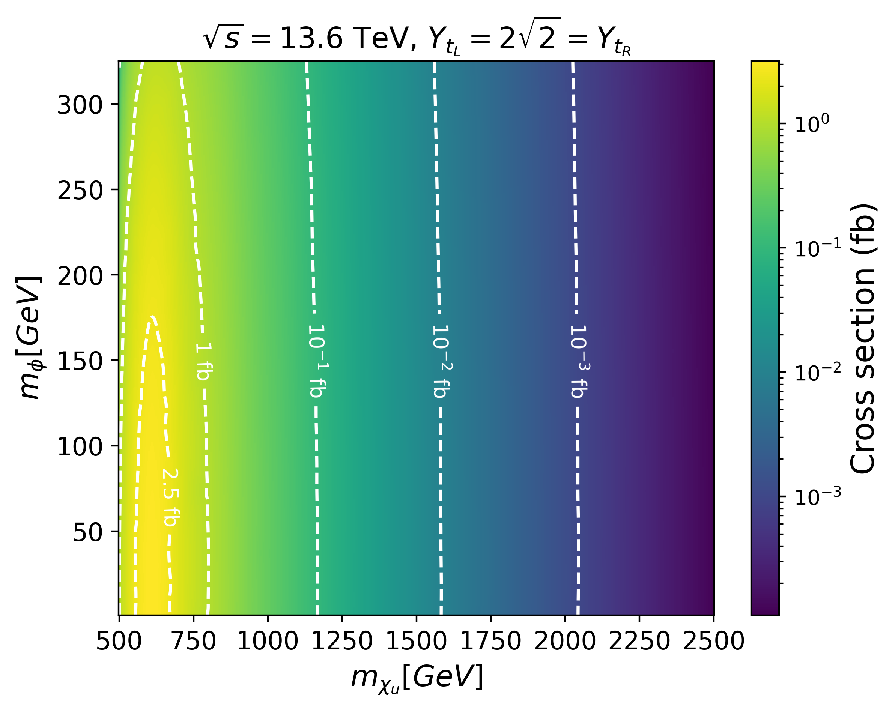
\includegraphics[width=0.85\linewidth]{Images/cross_section_by_masses.pdf}
    \caption{Projected cross section (fb) plot for $pp\to t \chi_\mathrm{u} \phi'$ and subsequent decay as a function of $m(\chi_\mathrm{u})$ and $m(\phi')$.}
    \label{fig:xs-plot}
\end{figure}

\begin{table}[]
  \begin{tabular}{l r}
    \hline
    {Background Process} & {Cross-Section $\sigma$ [\textrm{pb}]} \\
    \hline
   $\mathrm{pp} \to \mathrm{t} \overline{\mathrm{t}} \, \mu^+ \mu^-$ & $2.574\times 10^{-3}$  \\
    $\mathrm{pp} \to \mathrm{b}\overline{\mathrm{b}}\, \mu\mu\mu\nu $ & $4.692 \times 10^{-4}$ \\
    \hline
  \end{tabular}
  \centering
  \caption{A summary of dominant SM backgrounds produced by $\mathrm{pp}$ collisions and their cross sections in pb, as computed by \texttt{MadGraph} with $n = 10^6$ events.}
  \label{tab:dominantbkgs}
\end{table}

\begin{figure}[]
\centering
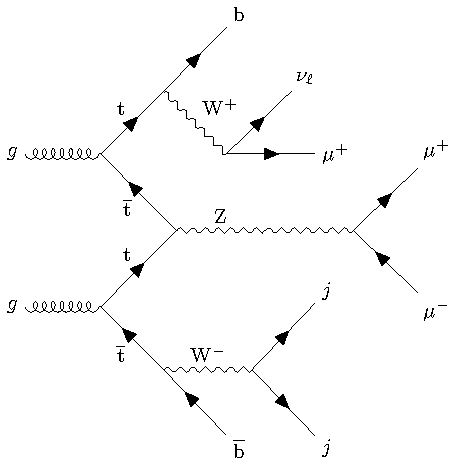
\includegraphics[width=.75\linewidth]{Images/bg_Z_full.pdf}
\caption{Representative Feynman diagram for a background event. A $Z$ boson is produced in association with a top quark through the fusion of a top, anti top pair from incoming protons. The $Z$ boson subsequently decays to a pair of muons and the two spectator top quarks decay semi-leptonically and purely hadronically to muons, neutrinos and jets, resulting in the same final states as the signal event.\label{fig:v}}
\end{figure}

\section{Discussion and conclusions}
\label{sec:discusion}

Experimental searches for $\lq$s with preferential couplings to third generation fermions are currently of great interest due to their potential to explain observed tensions in the $R_D$ and $R_{D^*}$ decay ratios of $\Bm$ mesons with respect to the SM predictions. Although the LHC has a broad physics program on searches for $\lq$s, it is very important to consider the impact of each search within wide range of different theoretical assumptions within a specific model. In addition, in order to improve the sensitivity to detect possible signs of physics beyond the SM, it is also important to strongly consider new computational techniques based on machine learning (ML). Therefore, we have studied the production of $U_1$ $\lq$s with preferential couplings to third generation fermions, considering different couplings, masses and chiral currents. These studies have been performed considering $\mathrm{p}\,\mathrm{p}$ collisions at $\sqrt{s} = 13\tev$ and $13.6\tev$ and different luminosity scenarios, including projections for the high luminosity LHC. A ML algorithm based on boosted decision trees is used to maximize the signal significance. The signal to background discrimination output of the algorithm is taken as input to perform a profile binned-likelihood test statistic to extract the expected signal significance. 

The expected signal significance for s$\lq$, d$\lq$ and non-res production, and their combination, is presented as contours on a two dimensional plane of $g_U$ versus $M_U$. We present results for the case of exclusive couplings to left-handed, mixed, and exclusive right-handed currents. For the first two, the region of the phase space that could explain the $\Bm$ meson anomalies is also presented. We confirm the findings of previous works that the largest production cross-section and best overall significance comes from the combination of d$\lq$ and non-res production channels. We also find that the sensitivity to probe the parameter space of the model is highly dependent on the chirality of the couplings. Nevertheless, the region solving the $\Bm$-meson anomalies also changes with each choice, such that in all evaluated cases we find ourselves just starting to probe this region at large $M_U$.

Our studies compare our exclusion regions with respect to the latest reported results from the ATLAS and CMS Collaborations. The comparison suggests that our ML approach has a better sensitivity than the standard cut-based analyses, especially at large values of $g_U$. In addition, our projections for the HL-LHC cover the whole region solving the B-anomalies, for masses up to $5.00\tev$.

Finally, we consider the effects of a companion $\zb^{\prime}$ boson on non-res production. We find that such a contribution can have a considerable impact on the LQ sensitivity regions, depending on the specific masses and couplings. In spite of this, we still consider non-res production as an essential channel for probing LQs in the future.

 %vectorial leptoquarks p p > ta+ ta- + bjets
% \chapter{ Probing Light Scalars and Vector-like Quarks at the High-Luminosity LHC}

% \section{Introduction}
% \label{introduction}


The Standard Model (SM) of particle physics, despite its successful account of numerous experimental findings involving strong, electromagnetic, and weak interactions, confirmed by CERN's Large Hadron Collider (LHC) is regarded as a lower-energy manifestation of a more comprehensive theory. This perspective arises from unresolved questions regarding the origins of dark matter, electroweak symmetry breaking scales, lepton flavor universality, the anomalous muon magnetic moment~\parencite{PhysRevD.73.072003, g2cit,Davier2017,Davier2020,PhysRevLett.121.022003,PhysRevD.97.114025,PhysRevLett.124.132002,PhysRevD.100.076004}, discrepancies in the $R_{(D)}$ and $R_{(D^{*})}$ ratios from $\mathrm{b}$-meson decays~\parencite{ BaBar:2012obs,BaBar:2013mob, Huschle:2015rga,LHCb:2015gmp,Aaij:2015yra,Sato:2016svk, Hirose:2016wfn, Aaij:2017uff, Hirose:2017dxl,LHCb:2017rln,Abdesselam:2019dgh,Belle:2019rba,LHCb:2023zxo}, as well as theoretical conundrums about whether gravity should be quantized, how gauge interactions can be unified, and the fine-tuning problem associated with the Higgs boson mass. Furthermore, the SM offers no explanation for fermion family replication nor for the lack of CP violation in the strong sector. These theoretical gaps, coupled with the experimental observation of phenomena such as neutrino masses, dark matter, and the baryon asymmetry in the universe, which cannot be explained by the SM, reinforce the expectation for physics beyond the SM (BSM).

As a result, several theoretical models have been put forth to address the limitations of the SM over the past decade. Despite differing theoretical motivations and resulting implications, a common thread among these ideas is the introduction of new particles, that, depending on the model, might be probed via proton-proton $(\mathrm{pp})$ collisions at the  LHC. A myriad of ideas have been suggested to investigate BSM physics, driving a substantial amount of exploration at the LHC. Said research has significantly limited the scope of theories and established exclusion bounds, extending to multi-\textrm{TeV} ranges for the masses of newly predicted particles within certain models~\parencite{ParticleDataGroup:2024cfk, CMS:2018iye, CMS:2016ucr, CMS:2016xbv, CMS:2016fxb, CMS:2017xcw, CMS:2015jsu}. Possible reasons for the absence of evidence could be attributed to new particle masses being at the scale where they are too large to be produced at the LHC energies and likely with exceptionally low production rates. In the scenario where the masses of the new particles might be probed at the LHC, a vast amount of data might be needed, together with advanced analysis techniques, to enhance the probability of detection. Alternatively, it is conceivable that new physics diverges from the conventional assumptions made in many BSM theories and the associated explorations. As a result, these new physics phenomena could remain hidden in processes that have not yet been thoroughly examined.


Minimal extensions to the SM, considering new $U(1)_{\chi}$ symmetry groups, are among the most studied BSM scenarios. For example, the  $U(1)_{T^3_R}$ symmetry, where families of right-handed fermions of the SM and possible extensions, such as right-handed neutrinos, are charged, was originally studied in the context of left-right symmetry models~\parencite{PatiSalam1974, MohapatraPati1975, SenjanovicMohapatra1975}. In these studies, $U(1)_{T^3_R}$ is identified as the subgroup of $SU(2)_R$ defined by its diagonal (electric-charge neutral) generator, $T^3_R$. In addition, it is often suggested that  $U(1)_{T^3_R}$ is a subspecies of a $U(1)_{B-L}$ symmetry since the breaking of the $U(1)_{B-L} \times U(1)_{T^3_R}$ leads to the $ U(1)_Y$ symmetry. This naturally motivates the presence of a massive and electrically neutral $\textrm{Z}'$ gauge boson~\parencite{DiLuzio2018, Baker2019, Michaels:2020fzj, Dev:2021otb, Florez2023}. However, in the breaking of  $U(1)_{B-L} \times U(1)_{T^3_R} \rightarrow U(1)_Y$, it follows that the Higgs doublet $\mathrm{H}$, since it is a singlet of $U(1)_{B-L}$,  acquires its hypercharge by inheritance from a charge under $U(1)_{T^3_R}$. Consequently, the vacuum expectation value (VEV) of $\mathrm{H}$  couples both symmetry-breaking scales for $U(1)_Y$ and $U(1)_{T^3_R}$. Alternatively, these symmetry-breaking scales can be decoupled by adding an additional $U(1)_G$ group where fermions of the SM are singlets and $\mathrm{H}$ is not. Therefore, the hypercharge comes from $U(1)_G$ for the $\mathrm{H}$ and from $U(1)_{T^3_R}$ for fermions, \textit{i.e.} $Y=Q_{T^3_R}+\frac{1}{2}Q_{B-L} + Q_G$~\parencite{Dutta:2022qvn}. Moreover, one can ask for scenarios where the hypercharge is not related to the $U(1)_{T^{3}_{R}}$ charge. 

Recently, theoretical and phenomenological efforts have emerged around scenarios where the low-energy gauge symmetry of the SM is extended by appending the Abelian gauge group $U(1)_{T^{3}_{R}}$, whose spontaneous symmetry-breaking is not linked to the electroweak one~\parencite{Dutta2019, Dutta2020, Dutta2020b,Dutta2022, PhysRevD.107.095019, Dutta2023}. In these scenarios, the gauge boson of $U(1)_{T^3_R}$ is associated with a massive dark photon $A'$ whose longitudinal mode arises from a Higgs-like mechanism involving a complex scalar field, $\phi$. This field is a singlet under the SM group, with its CP-odd component associated with the $A'$ mass and the CP-even giving rise to a dark Higgs, $\phi'$. To cancel gauge anomalies, a right-handed $\nu_R$ neutrino must be included for each generation of the SM that couples to $U(1)_{T^3_R}$. Furthermore, to correctly explain the origin of fermion masses in a UV-complete theory, a set of new vector-like quarks $(\chi_\mathrm{u}, \chi_d,\chi_\ell, \chi_\nu)$ must be included. These new particles are singlets under $U(1)_{T^3_R}$ and charged like SM right-handed fermions, as in the universal see-saw mechanism~\parencite{Berezhiani, Chang1987, Davidson1987, Rajpoot1987, Babu1989, Babu1990}.

In this phenomenology study, we devise a LHC search strategy for the light \textrm{GeV}-scale scalar boson $\phi'$ produced in association with a heavy \textrm{TeV}-scale $\chi_\mathrm{u}$, the partner particle of the top quark, through a previously unexplored production and final state channel. Particularly, we explore the production of $\mathrm{pp}\to \mathrm{t}\chi_\mathrm{u} \phi'$, in contrast to $\mathrm{pp}\to \mathrm{T}\mathrm{T}\to \mathrm{t}\phi'\mathrm{t}\phi'$ with hadronic~\parencite{Bhardwaj_2022, Bhardwaj_2022_2, Bardhan_2023} di-photonic $\phi'$~\parencite{Banerjee_2016, Alves_2024} decays. Due to the non-trivial $\chi - \mathrm{t} -\phi'$ coupling, processes where the final state includes $ \mathrm{t}\chi_\mathrm{u} \phi'$ are allowed in \textrm{pp} colliders through the ${\chi_\mathrm{u}}{- \mathrm{t}}$ fusion, see Figure~\ref{fig:qqfusion}. Since the $\chi_\mathrm{u}$ couples to SM quarks and gluons, it can be produced in large quantities. Furthermore, its energetic decay products can be detected alongside the $\phi'$ mediator particle that has significant transverse momentum. Therefore, if the $\phi'$ decays into SM particles that are observable in the detector's central region, this strategy can be very effective at reducing the SM background, and thus improve the long-term LHC discovery reach for heavy top partners and~\textrm{GeV}-scale mediators, which are typically hard to detect using conventional methods at hadron colliders. Moreover, since it is possible to have $\chi_\mathrm{u} \to \mathrm{t}\,\phi'$ decays (and $\bar{\chi_\mathrm{u}} \to \bar{\mathrm{t}}\,\phi'$), the same $\mathrm{pp}\to \mathrm{t}\chi_\mathrm{u} \phi'$ state may arise from $\chi_\mathrm{u}\bar\chi_\mathrm{u}$ production diagrams with quantum chromodynamic (QCD) vertices, where one $\chi_\mathrm{u}$ decays to $\mathrm{t}\phi'$, 
as shown in Figure~\ref{fig:ggfusion}. As a consequence, the energetic products from $\chi_\mathrm{u}\bar\chi_\mathrm{u}$ decays can be readily detected, particularly when they occur alongside a mediator particle that carries substantial transverse momentum, providing greater sensitivity than that of searches where either $\chi_\mathrm{u}$ or $\phi'$ are considered in isolation. 

We probe the scenario where the scalar $\phi'$ has family non-universal fermion couplings, as was suggested in~\parencite{Dutta2020}, and thus can address several issues with the SM. 
We focus on the $\phi^{\prime}$ decay to a pair of muons since, at the experimental level, muons generally have high reconstruction and identification efficiencies, which allow for the development of relatively low $p_{\mathrm{T}}(\mu)$ triggers, and provide clean signatures to remove the copious QCD multijet SM background. A key component of this study is the development of an analysis strategy utilizing a machine learning (ML) algorithm based on Boosted Decision Trees (BDT)~\parencite{friedman_greedy_2001}. The event classifier's output is employed to conduct a profile-binned likelihood test, which is used to determine the overall signal significance for each model examined in the analysis. The effectiveness of BDTs and other ML algorithms has been validated in numerous experimental and phenomenological studies~\parencite{,Ai:2022qvs, ATLAS:2017fak, Biswas:2018snp,  Chung:2020ysf, Feng:2021eke, ttZprime, Chigusa:2022svv,  Florez2023, Arganda2024, Ajmal_2024, Dutta_2015}. Our findings indicate that the BDT algorithm significantly enhances signal significance.

The rest of this paper is structured as follows. Section~\ref{sec:model} discusses details of the minimal  $U(1)_{T_R^3}$ model. Section~\ref{sec:exp} provides an overview of current relevant results at the LHC. Section~\ref{sec:sims} explains how the Monte
Carlo (MC) simulation samples are produced for this study. In Section~\ref{sec:ML} we discuss the motivation and details of our machine learning workflow, and in Section~\ref{sec:results}, the main results are presented. We conclude with a short discussion in Section~\ref{sec:discussion}.
\begin{figure}
    \centering
    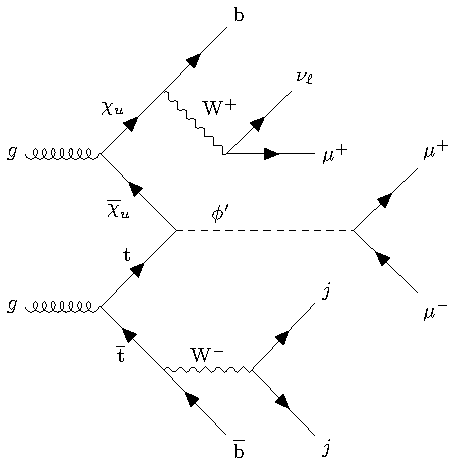
\includegraphics[width=0.85\linewidth]{Images/signal_qqfusion.pdf}
    \caption{Representative Feynman diagram for the production of a $\phi'$ boson in association with a $\chi_\mathrm{u}$ vector-like quark through the fusion of a top quark and $\chi_\mathrm{u}$ vector-like quark. Once again, the $\phi'$ decays to a pair of muons, the top quark decays fully hadronically, and the $\chi_\mathrm{u}$ decays semi-leptonically to muons, neutrinos and $b$-jets.\label{fig:qqfusion}}
\end{figure}

\begin{figure}
    \centering
    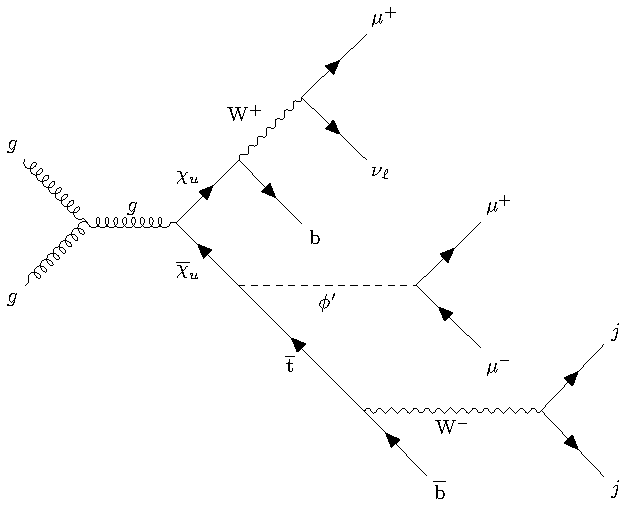
\includegraphics[width=0.85\linewidth]{Images/signal_ggfusion.pdf}
    \caption{Representative Feynman diagram for the production of a $\phi'$ boson in association with a $\chi_\mathrm{u}$ vector-like quark through the fusion of a gluon pair from incoming protons. The $\phi'$ decays to a pair of muons, the top quark that decays fully hadronically, and the $\chi_\mathrm{u}$ decay semi-leptonically to muons, neutrinos and jets.\label{fig:ggfusion}}
\end{figure}

\section{Experimental Considerations}\label{sec:exp}

The ATLAS and CMS collaborations at CERN have conducted various searches for heavy vector-like quarks (T). These searches utilized $\mathrm{pp}$ collisions at center-of-mass energies of $\sqrt{s} = 8$ and $13$ \textrm{TeV}. The studies primarily focused on T production through gluon-mediated QCD processes, either in pair production from quark-antiquark annihilation (Figure~\ref{fig:qcd_T_prod}) or in single-T production from electroweak processes involving associated quarks (Figure~\ref{fig:qed_T_prod}). 

\begin{figure}
\centering
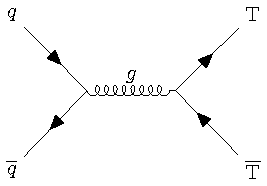
\includegraphics[width=0.65\linewidth]{Images/T_prod_qcd.pdf}
\caption{Representative Feynman diagram for T pair production via gluon-mediated QCD processes.\label{fig:qcd_T_prod}}
\end{figure}

\begin{figure}
\centering
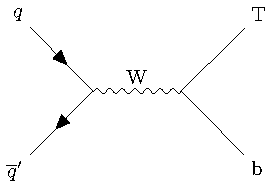
\includegraphics[width=0.65\linewidth]{Images/T_prod_qed.pdf}
\caption{Representative Feynman diagram for single T production via electroweak processes.\label{fig:qed_T_prod}}
\end{figure}


In those studies, \textrm{T} decays into $\mathrm{bW}$, $\mathrm{tZ}$, or $\mathrm{tH}$ have been considered. In the context of \textrm{T} pair production, $\mathrm{T}\bar{\mathrm{T}}$, via QCD processes, the cross sections are well-known and solely depend on the mass of the vector-like quark.  Assuming a narrow $\mathrm{T}$ decay width ($\Gamma / m(\mathrm{T}) < 0.05$ or 0.1) and a 100\% branching fraction to $\textrm{bW}$, $\textrm{tZ}$, or $\textrm{tH}$, these searches have set stringent bounds on $m(\mathrm{T})$, excluding masses below almost 1.5 \textrm{TeV} at 95\% confidence level~\parencite{CMS:2024bni,CMS:2024qdd,ATLAS:2022ozf,ATLAS:2023bfh,ATLAS:2022hnn,ATLAS:2022tla,ATLAS:2023pja,ATLAS:2024fdw}. The most recent analysis from the CMS collaboration probes T-quark production via $\mathrm{pp} \to \mathrm{T}\textrm{qb}$, in final states with $\mathrm{T} \to \textrm{tZ}$ or $\mathrm{T} \to \textrm{tH}$, considering scenarios with preferential couplings to third-generation fermions. The analysis sets 95\% confidence level upper limits of 68-1260 \textrm{fb} on the production cross section, for T masses ranging from 600-1200 \textrm{GeV}~\parencite{CMS:2024qdd}. The latest studies from ATLAS probe vector-like quarks using the single-T production mode with the $\mathrm{T} \to \textrm{tH}$ decay channel leading to a fully hadronic final state~\parencite{ATLAS:2022ozf}, the single-T production mode with the $\mathrm{T} \to \textrm{tZ}$ decay channel leading to a multileptonic final state~\parencite{ATLAS:2023bfh}, the TT pair production mode with various T decay channels leading to multileptonic final states~\parencite{ATLAS:2022hnn}, and the TT pair production mode with various T decay channels leading to a single lepton plus missing momentum final state~\parencite{ATLAS:2022tla,ATLAS:2023pja}. 
The multilepton search offers the greatest sensitivity in most of the phase space, but the missing transverse energy based search has better sensitivity for low branching fraction $\mathfrak{B}(\mathrm{T}\to \textrm{Wb})$ and high $\mathfrak{B}(\mathrm{T}\to \textrm{Ht})$. These searches have similar sensitivities for the singlet and doublet models, resulting in exclusion bounds for masses below about 1.25 \textrm{TeV} and 1.41 \textrm{TeV}, respectively. 


A key consideration in the model interpretations summarized above is that the $\mathrm{T}$ branching fractions depend on the chosen model. The excluded mass range is less restrictive for specific branching fraction scenarios, such as $\{\mathfrak{B}(\mathrm{T} \to \textrm{tZ})$, $\mathfrak{B}(\mathrm{T} \to bW)$, $\mathfrak{B}(\mathrm{T} \to \textrm{tH})\}= \{0.2, 0.6, 0.2\}$, excluding masses below about 0.95 \textrm{TeV}. Moreover, if the $\mathrm{T} \to \phi't $ decay is allowed, or if the branching fractions $\mathfrak{B}(\mathrm{T} \to \textrm{tH/bW})$ are lower, the limits previously quoted must be re-evaluated. The authors of Ref.~\parencite{Cacciapaglia:2019zmj} emphasize that bounds on $m(\mathrm{T})$ can be around 500 \textrm{GeV} when $\mathrm{T} \to \mathrm{t}\phi'$ decays are permitted. Therefore, to facilitate a comprehensive study, benchmark scenarios in this paper are considered down to $m(\chi_\mathrm{u}) = 500$ \textrm{GeV}.

\section{\boldmath The Minimal $U(1)_{T_R^3}$ Model}\label{sec:model}
\subsection{Scalar Potential}
In this model, the SM is extended by the Abelian gauge symmetry $U(1)_{T^3_R}$, where only right-handed fermions are charged. We assume two independent Higgs mechanisms, one with a Higgs doublet $\mathrm{H}$ for electroweak symmetry breaking and the other with a Higgs singlet $\phi$ for the $U(1)_{T^3_R}$ symmetry breaking. Both scalars have independent vacuum expectation values (VEVs), $\expval{H}=v_h/\sqrt2$ and $\expval\phi =v_\phi/\sqrt2$, allowing us to express the doublet and singlet Higgs fields, following a Kibble parametrization, as 
\begin{align}
    H & = \begin{pmatrix}
        G_{+} \\
        \frac{1}{\sqrt{2}}\left(v_h+\rho_0+i G_{0}\right)
    \end{pmatrix}\label{eq:higgskibblepara1}
    \\
    \phi & =\frac{1}{\sqrt{2}}\left(v_\phi + \rho_\phi+i G_{\phi}\right). \label{eq:higgskibblepara2}
\end{align}
In Eqs.\ref{eq:higgskibblepara1} and Eq.\ref{eq:higgskibblepara2}, $G_\pm$, $G_0$, and $G_\phi$ are the Goldstone bosons that allow the SM $\textrm{W}^\pm$ and $\textrm{Z}$ bosons and the dark photon $A'$, associated with the $U(1)_{T^3_R}$ symmetry, to acquire mass. The $\rho_h$ and $\rho_\phi$ are an orthogonal mixture of the SM Higgs boson and the dark Higgs
\begin{equation}
    \begin{pmatrix}
        h
        \\
        \phi'
    \end{pmatrix}
    =
    \begin{pmatrix}
        \cos\alpha & -\sin\alpha
        \\
        \sin\alpha & \cos\alpha
    \end{pmatrix}
    \begin{pmatrix}
        \rho_0
        \\
        \rho_\phi
    \end{pmatrix},
\end{equation}
that results from the diagonalization of the mass matrices arising from the gauge invariant potential
\begin{equation}
    \begin{aligned}
        \mathcal V(\phi,H)
    &= \mu_H^2 H^{\dagger} H 
    +\mu_\phi^2 \phi^* \phi
    \\
    &+\lambda\left(H^{\dagger} H\right)\left(\phi^* \phi\right)
    +\lambda_H\left(H^{\dagger} H\right)^2
    +\lambda_\phi\left(\phi^* \phi\right)^2.
    \end{aligned}
\end{equation}
The tadpole equations are given from the minimization of the potential as
\begin{align}
    \pdv{\mathcal V}{H} 
     &= \frac{v_h}{\sqrt2} \left( \mu_H^2 +\lambda_Hv_h^2 + \frac{1}{2} \lambda v_\phi^2 \right) = 0,
    \\
    \pdv{\mathcal V}{\phi}
    &= \frac{v_\phi}{\sqrt2} \left( \mu_\phi^2 +\lambda_\phi v_\phi^2 + \frac{1}{2} \lambda v_h^2 \right) = 0.
\end{align}
The masses of the scalar bosons can be written as
\begin{equation}
    \begin{aligned}
        m_{h,\phi'}^2 &= \frac{1}{2}\left( 
    \lambda_H v_h^2 + \lambda_\phi v_\phi^2
    \right)\\
    &\pm 
    \sqrt{
        \lambda^2 v_h^2 v_\phi^2
        +
        \left(
        \lambda_H v_h^2 - \lambda_\phi v_\phi^2
        \right)^2
    },
    \end{aligned}
\end{equation}
and the mixing angle $\alpha$ as
\begin{equation}
    \tan \alpha = \frac{-\lambda v_h v_\phi}{ \lambda_H v_h^2 - \lambda_\phi v_\phi^2 - \sqrt{\lambda^2 v_h^2 v_\phi^2 + \left(\lambda_H v_h^2 - \lambda_\phi v_\phi^2\right)^2}}.
\end{equation}

\subsection{The Universal Seesaw Mechanism}
In the model, each electrically charged SM fermion $f$ has a mass protected by both VEVs. In turn, they  acquire mass from the mixture with a vector-like fermion $\chi_f$, which is charged as the right-handed component of the respective SM fermion, in a UV complete theory. The terms in the Lagrangian density that contribute to the mass of physical fermions are,
\begin{equation}
    \begin{aligned}
        -\mathcal{L}&\supset 
    Y_{f_L} \bar{f}_L' \chi_{fR}' H 
    +Y_{f_R} \bar\chi_{fL}' f'_R  \phi^* 
    + m_{\chi_f'} \bar{\chi}_{f L}' \chi_{f R}'\\
&+\text { h.c.}
    \end{aligned}
\end{equation}
Therefore, in the vacuum, the mass matrix is
\begin{equation}
    M_f=
    \begin{pmatrix}
    0 & Y_{f_L} v_h /\sqrt2\\
    Y_{f_R} v_\phi /\sqrt2 & m_{\chi_f'}    
    \end{pmatrix}.
\end{equation}
The left- and right-handed components of the physical fermions $(f,\,\chi_f)$ are given by two rotations $\mathcal R(\theta_{f_{L,R}})$ as, 
\begin{equation}
    \begin{pmatrix}
        f_{L,R}
        \\
        \chi_{f_{L,R}}
    \end{pmatrix}
    =
    \begin{pmatrix}
        \pm\cos\theta_{f_{L,R}} & \mp \sin \theta_{f_{L,R}}
        \\
        \sin \theta_{f_{L,R}} & \cos\theta_{f_{L,R}}
    \end{pmatrix}
    \begin{pmatrix}
        f_{L,R}'
        \\
        \chi_{f_{L,R}}'
    \end{pmatrix},
\end{equation}
in a way that $\mathcal{R}(\theta_{f_L})M_f\mathcal{R}^{-1}(\theta_{f_R})=\text{diag}(m_f,m_{\chi_f})$ up to a phase. Assuming real parameters, the physical masses and the mixing angles are given by
\begin{gather}
    m_f m_{\chi_f}=\frac{ \left(Y_{f_{L}} v_h\right) \left(Y_{f_R} v_\phi\right)}{2}, \label{eq:prodmass}
     \\ 
    m_f^2 + m_{\chi_f}^2 = m_{\chi_f'}^2 + \frac{1}{2}\left(Y_{f_L}^2v_h^2+Y_{f_R}^2v_\phi^2\right),\label{eq:summass}
    \\
    \tan \theta_{f_{L,R}} =  \frac{\sqrt 2}{m_{\chi_f'}}\left(\frac{Y_{f_{L,R}}v_{h,\phi}}{2} - 
    \frac{m_f^2}{Y_{f_{L,R}}v_{h,\phi}} \right).
\end{gather}

\noindent The Yukawa interactions of the physical fermions with the scalar bosons have the form
\begin{equation}
    -\mathcal{L}_{\text{yuk}} 
    = h \bar\psi_{f_L} \mathcal{Y}_{h}\psi_{f_R} + \phi' \bar\psi_{f_L} \mathcal{Y}_{\phi}\psi_{f_R},
\end{equation} 
with $\psi_{f} = (f,\chi_{f})^T$, and the matrices $\mathcal{Y}_{f_{L,R}}$ given by
\begin{align}
    \mathcal{Y}_{h} &= \frac{1}{\sqrt{2}}
    \mathcal{R}(\theta_{f_L})
    \left(
        Y_{f_L}\sigma_+ \cos\alpha 
    - 
    Y_{f_R}\sigma_-\sin\alpha
    \right)
    \mathcal{R}^{-1}(\theta_{f_R})\label{eq:YukawaL}
    \\
    \mathcal{Y}_{\phi} &= \frac{1}{\sqrt{2}}
    \mathcal{R}(\theta_{f_L})
    \left(
    Y_{f_L}\sigma_+ \sin\alpha
    +
    Y_{f_R}\sigma_-\cos\alpha
    \right)
    \mathcal{R}^{-1}(\theta_{f_R}),\label{eq:YukawaR}
\end{align}
where $\sigma_{\pm}=(\sigma_1\pm i\sigma_2)/2$ are the ladder Pauli matrices.

\subsection{Minimal UV-complete theory}

The model must provide non-zero masses for all the SM fermions and be free of gauge anomalies. So, we must have at least one full generation of vector-like fermions $\{\chi_\mathrm{u}$, $\chi_\mathrm{d}$, $\chi_\mathrm{\ell}$, $\chi_\mathrm{\nu}\}$ and the right-handed component of the SM neutrinos, $\nu_R$, charged as shown in Table~\ref{tab:QMnumbers}. Therefore, the Yukawa interactions in the UV-complete theory must be of the form
\begin{equation}
    \begin{aligned}
        -\mathcal{L}
        \supset&\quad
        Y_{L u}^i \bar{q}_L^{\prime i} \chi_{u R}' \widetilde{H}
        + Y_{R u}^i \bar{\chi}_{u L}' u_R^{\prime i} \phi^*  
        + m_{\chi_\mathrm{u}} \bar{\chi}_{u L}' \chi_{u R}'
        \\&
        +Y_{L d}^i \bar{q}_L^{\prime i} \chi_{d R}' H 
        +Y_{R d}^i \bar{\chi}_{d L}' d_R^{\prime i} \phi
        +m_{\chi_d} \bar{\chi}_{d L}' \chi_{d R}'
        \\&
        +Y_{L \ell}^{i} \bar{\ell}_L^{\prime i} \chi_{\ell R}' H
        +Y_{R \ell}^{i} \bar{\chi}_{\ell L}' \ell_R^{\prime i} \phi
        +m_{\chi_\ell} \bar{\chi}_{\ell L}' \chi_{\ell R}'
        \\
        &
        +Y_{L \nu}^{i} \bar{\ell}_L^{\prime i} \chi_{\nu R}' \widetilde{H}
        +Y_{R \nu}^{i} \bar{\chi}_{\nu L}' \nu_R^{\prime i} \phi^*
        +m_{\chi_\nu} \bar{\chi}_{\nu L}' \chi_{\nu R}' \\
        &+\text { h.c., }
    \end{aligned}
\end{equation}
where the $i$ index runs over the three generations of fermions. The simultaneous diagonalization of the mass matrices of each fermion sector will have a similar structure to the one presented in Eqs.~\ref{eq:prodmass} and~\ref{eq:summass} and the Yukawa matrices will have a similar structure of Eqs.~\ref{eq:YukawaL} and~\ref{eq:YukawaR} but codifying the $CKM$ matrix. For the neutrino sector, the structure of the mass matrix will be more complicated due to the presence of the additional Majorana mass term for the vector-like neutrino $\chi_\nu'$.

\begin{table}[h]
    \centering
    \begin{tabular}{ccccc}
    \hline
    \hline
        Field & $SU(3)_C$  & $SU(2)_L$ & $U(1)_Y$ & $U(1)_{T^3_R}$ \\
    \hline\hline
        $q_L'$                    & \bf{3} & \bf{2} & 1/6 & 0\\
        $\ell_L'$                 & \bf{1} & \bf{2} & -1/2 & 0\\
        $H$                         & \bf{1} & \bf{2} & 1/2 & 0\\
        \hline
        $u_R^{\prime c}$          & \bf{3} & \bf{1} & -2/3 & -2\\
        $d_R^{\prime c}$          & \bf{3} & \bf{1} & 1/3 & 2\\
        $\ell_R^{\prime c}$       & \bf{1} & \bf{1} & 1 & 2\\
        $\nu_R^{\prime c}$        & \bf{1} & \bf{1} & 0 & -2\\
        $\phi$                      & \bf{1} & \bf{1} & 0 & 2\\
        \hline
        $\chi_{u_L}'$               & \bf{3} & \bf{1} & 2/3 & 0\\
        $\chi_{u_R}^{\prime c}$     & \bf{3} & \bf{1} & -2/3 & 0\\
        $\chi_{d_L}'$               & \bf{3} & \bf{1} & -1/3 & 0\\
        $\chi_{d_R}^{\prime c}$     & \bf{3} & \bf{1} & 1/3 & 0\\
        $\chi_{\ell_L}'$            & \bf{1} & \bf{1} & -1 & 0\\
        $\chi_{\ell_R}^{\prime c}$  & \bf{1} & \bf{1} & 1 & 0\\
        $\chi_{\nu_L}'$             & \bf{1} & \bf{1} & 0 & 0\\
        $\chi_{\nu_R}^{\prime c}$   & \bf{1} & \bf{1} & 0 & 0\\
    \hline
    \hline
    \end{tabular}
    \caption{Minimal field content of the model and their representations under the SM and $U(1)_{T^3_R}$ gauge groups.}
    \label{tab:QMnumbers}
\end{table}

\section{Samples and Simulation}\label{sec:sims}
The minimal $U(1)_{T^3_R}$ model described in Sec.~\ref{sec:model} is implemented into the \texttt{FeynRules} package~\parencite{Alloul:2013bka}, which generates the Feynman rules and exports them into a Universal \texttt{FeynRules} Output (\texttt{UFO})~\parencite{Degrande:2011ua}. The resulting \texttt{UFO} is utilized as input for a generator to produce the MC samples. Both signal and background events are generated with the \texttt{MadGraph5\_aMC@NLO} v3.2.0 program~\parencite{Alwall:2014hca,Alwall:2014bza} at leading order (LO) in QCD, considering \textrm{pp} beams colliding with a center-of-mass energy of $\sqrt{s} = 13.6$ \textrm{TeV}. Each signal and background sample is generated separately, with no interference effects between the signal and background considered. The impact of these interference effects has been evaluated, and for all values of $\chi_\mathrm{u}$ and $\phi'$ masses considered, the effect on the signal plus background cross section is found to be less than $<0.5$\%. Additionally, the effect on the shape of the b-jet $p_{T}$ distribution is less than 6\% for $p_{T} < 300$ GeV and less than 2\% for b-jet $p_{T} > 300$ GeV. We use the \texttt{NNPDF3.0~NLO}~\parencite{NNPDF:2014otw} set for parton distribution functions (PDFs) for all event generation. Parton-level events are then interfaced with \texttt{PYTHIA} (v8.2.44)~\parencite{Sjostrand:2014zea} to account for parton showering and hadronization processes. Finally, we use  \texttt{DELPHES} (v3.4.2)~\parencite{deFavereau:2013fsa} to simulate smearing and other detector effects using the CMS detector geometric configurations and parameters for particle identification and reconstruction, using the CMS input card with 140 average pileup interactions. All signal cross sections used in this analysis are obtained requiring the following kinematic criteria on leptons $\ell$, \textrm{b} quarks, and light-quark/gluon jets ($j$) at parton level in \texttt{MadGraph}: $p_{\mathrm{T}}(\ell) > 35$~\textrm{GeV}, $\abs{\eta (\mathrm{b})} < 2.5$, $\abs{\eta (\ell)} < 2.3$, $p_{\mathrm{T}}(j) > 20$~\textrm{GeV}, and $\abs{\eta (\mathrm{j})} < 5$. These parton-level selections were applied exclusively to the signal processes to restrict event generation to the relevant phase space regions. For background processes, these default parton level requirements in \texttt{MadGraph} were imposed:  $p_{\mathrm{T}}(\ell) > 10$~\textrm{GeV}, $\abs{\eta (\ell)} < 2.5$, $p_{\mathrm{T}}(j) > 20$~\textrm{GeV}, $\abs{\eta (\mathrm{j})} < 5$, and $\abs{\eta (\mathrm{b})} < 5$. This ensures that the phase space regions for the background near the analysis-level selection criteria are adequately described after parton showering since the pre-selections at the analysis level are more stringent than the parton-level requirements. Furthermore, we use the MLM algorithm for jet matching and jet merging. The parameters \texttt{xqcut} and \texttt{qcut} of the MLM algorithm are set to 30 and 45 respectively to ensure continuity of the differential jet rate as a function of jet multiplicity. Each simulated signal and background sample is produced separately at LO, with one million events at the generation level, neglecting potential interference effects between the signal and background due to the suppression caused by the different orders of magnitude in the coupling constants of the signal and background.

Signal samples are generated considering the production of a $\phi'$ boson, an associated $\chi_\mathrm{u}$ vector-like quark, and a top quark $(\mathrm{pp}\to \chi_\mathrm{u} \mathrm{t} \phi')$, inclusive in both $\alpha$ and $\alpha_s$ (see Figures~\ref{fig:qqfusion}-\ref{fig:ggfusion}). We have used the implementation of the $U(1)_{T^3_R}$ model in Ref.~\parencite{Dutta2023}. Signal samples were created considering coupling values of $Y_{\mathrm{t}_R}=Y_{\mathrm{t}_L}=2\sqrt{2}$ in the range of masses $m(\phi')\in\{5,10,50,100,325\}$~\textrm{GeV} for the dark higgs and $m(\chi_\mathrm{u})\in\{0.50, 0.75, 1.0, 1.5, 2.0, $ $ 2.5\}$~\textrm{TeV} for the vector-like quark $\chi_u$~\parencite{PhysRevD.108.095006}. The production cross section for $\mathrm{pp}\to \chi_\mathrm{u} \mathrm{t} \phi'$ is highly dependent on the choice of the Yukawa couplings in the Lagrangian. The ${\chi_\mathrm{u}}{- \mathrm{t}}$ fusion process shown in Figure~\ref{fig:qqfusion} is dominated by the $Y_{\mathrm{t}_R}$ coupling. However, the decay ${\chi_\mathrm{u}} \to \mathrm{t} \phi'$ shown in Figure~\ref{fig:ggfusion} is inversely proportional to the $Y_{\mathrm{t}_L}$ coupling. This effect is shown in Figure~\ref{fig:cross_section_by_lambdas}, which displays the total signal cross section, as a function of $Y_{\mathrm{t}_R}$ and $Y_{\mathrm{t}_L}$, for a benchmark point with $m(\phi')=100$~\textrm{GeV} and $m(\chi_\mathrm{u})=1.0$~\textrm{TeV}. 

\begin{figure}
    \centering
    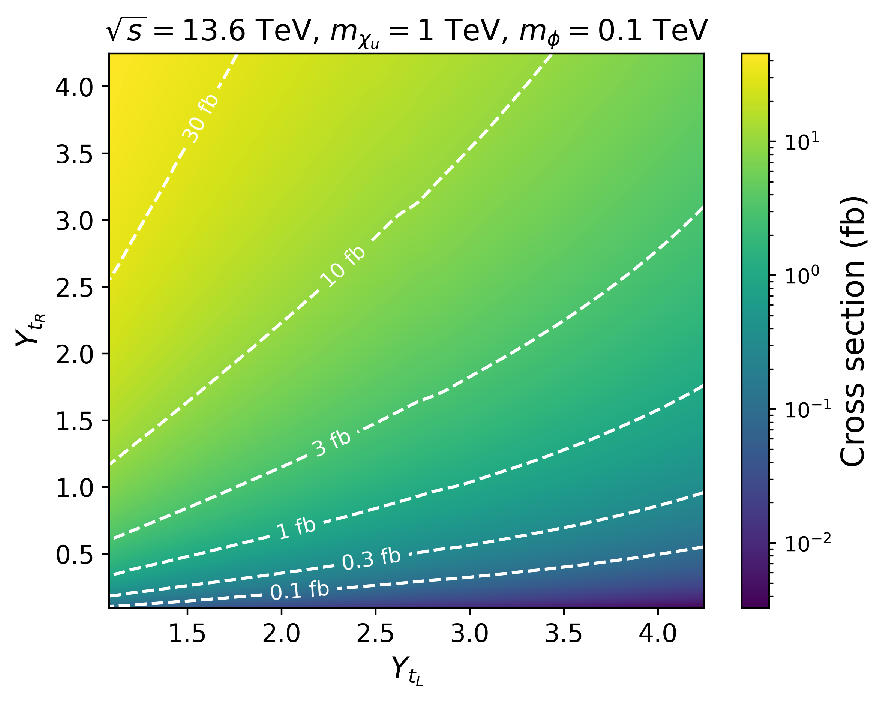
\includegraphics[width=0.85\linewidth]{Images/cross_section_by_lambdas.pdf}
    \caption{Signal production cross section, $ \mathrm{pp}\to \chi_\mathrm{u} \mathrm{t} \phi'$,  in the $Y_{\mathrm{t}_R}$ versus $Y_{\mathrm{t}_L}$ plane, for a benchmark point with $m(\phi')=100$~\textrm{GeV} and $m(\chi_\mathrm{u})=1.00$~\textrm{TeV}. The white-dashed contours show specific cross section values in the two dimensional plane.}
    \label{fig:cross_section_by_lambdas}
\end{figure}

We target signal events where the top quark decays hadronically into a bottom quark and two jets ($\mathrm{t} \to \mathrm{bW} \to \mathrm{b} q \bar{q}'$), the $\chi_\mathrm{u}$ decays semileptonically into a $b$ quark, lepton, and neutrino (via $\chi_\mathrm{u} \to \mathrm{bW}$ and $\mathrm{W}\to\mu\nu_{\mu}$), and the $\phi'$ produces two muons. We note that the scalar $\phi'$ particle could result from the mixture of the SM Higgs boson and additional scalar fields, and the Yukawas of the fermions could additionally arise from the mixing of the SM fermions with additional copies of the associated vector-like fermions. Therefore, the $\phi'$ branching ratios are dependent on the chosen mechanism and model by which this mixture occurs, see for example, Refs.~\parencite{Cacciapaglia_2023,Blankenburg:2012nx,Jones-Perez:2013oia,Calibbi:2009pv}. For the purpose of this work, and 
similar to Refs.~\parencite{Dutta2020,Dutta2023}, the considered benchmark signal scenarios have $\mathfrak{B}(\chi_\mathrm{u} \rightarrow \textrm{b W})$ of about 0.5 and $\mathfrak{B}(\phi' \rightarrow \mu^+\mu^-)=0.98$. Figure~\ref{fig:xs-plot} shows the production cross section in \textrm{fb}, as a function of $m(\phi')$ and $m(\chi_\mathrm{u})$ masses, assuming the aforementioned decays, branching ratios, and couplings.

We note that for the parameter space of focus in this paper, the total mass of the $t$-$\chi_\mathrm{u}$ system is larger than $m(\phi')$, thus the large rest energy of the $t$-$\chi_\mathrm{u}$ system is converted into potentially large momentum values for the $\phi'$. Similarly, the $t$-quark produced through the $\chi_\mathrm{u}$-$t$ fusion interaction can also have large momentum values, and thus in some cases the hadronic $t$ decay products cannot be fully reconstructed independently of each other. This results in three possible $t$ reconstruction scenarios: a fully merged scenario where the $\mathrm{W}\to jj$ system and the $\mathrm{b}$ quarks are very collimated and reconstructed as a single ``fat jet’’ (henceforth referred to as a FatJet, FJ); a partially merged scenario, where the decay products of the $\mathrm{W}$ boson form a single FatJet but the $\mathrm{b}$ quark can still be separately identified; and an un-merged scenario where all decay products can be independently identified. Jets are clustered using the anti-$k_t$ algorithm~\parencite{Cacciari_2008} using the \texttt{FastJet} (v3.4.2)~\parencite{Cacciari_2012} package with a distance parameter of $R = 0.4$ for standard jets and $R = 0.8$ for fat jet objects. Each scenario has an associated identification efficiency and misidentification rate, which depends on the choice of the boosted $t$/$W$ algorithm (our choice of efficiency and misidentification rates is described later). 

Based on the above details, the final state of interest in this paper consists of three muons (two from the $\phi'$ decay and one from the $\chi_\mathrm{u}$ decay), a (possibly boosted) top-tagged system, at least one $b$-tagged jet, and large missing transverse momentum ($\vec{p}_{T}^{\textrm{~miss}}$). For the partially merged and un-merged scenarios, there will be two $b$ quarks present in the final state (one of which is part of the top tagged system). 

We consider background sources from SM processes which can give similar objects in the final state as those expected for signal. Several background sources were considered and studied, such as QCD multijet events, production of vector boson pairs ($\mathrm{VV: WW, ZZ, WZ}$), vector boson triplets ($\mathrm{VVV: WWZ, WZZ, ZZZ, WWW}$), top-quark pairs in association with weak bosons ($\mathrm{t}\overline{\mathrm{t}}X$), and $\mathrm{t}\overline{\mathrm{t}}\mathrm{t}\overline{\mathrm{t}}$ processes. The  dominant sources of SM background events are from the $\mathrm{t}\overline{\mathrm{t}}X$, $\mathrm{ZZW}$, and $\mathrm{t}\overline{\mathrm{t}}\mathrm{t}\overline{\mathrm{t}}$ processes. The $\mathrm{t}\overline{\mathrm{t}}X$ background is primarily associated production of a $\mathrm{Z}/\gamma^{*}$ from $\mathrm{t}\bar{\mathrm{t}}$ fusion processes. The $\mathrm{ZZW}$ process becomes a background when one $\mathrm{Z}$ decays $\mathrm{b}\bar{\mathrm{b}}$, another $\mathrm{Z}$ decays to a pair of muons, and the W decays to a muon and a neutrino. 
Events from $\mathrm{ZZW}$ and $\mathrm{t}\overline{\mathrm{t}}\mathrm{t}\overline{\mathrm{t}}$ have been combined, after being weighted by their corresponding production cross section. The combination is presented as the ``$\mathrm{b} \overline{\mathrm{b}}\mu\mu\mu\nu$'' background in the remainder of this paper. The $\mathrm{t}\overline{\mathrm{t}}X$ process is presented as part of the ``$\mathrm{t}\overline{\mathrm{t}}\mu^{+}\mu^{-}$'' background. Table~\ref{tab:dominantbkgs} shows the production cross sections for the dominant background sources. The rest of the aforementioned background processes do not contribute meaningfully in our context, accounting for $\ll 1\%$ of the total expected background yield.

The identification of leptons, boosted top quarks, and bottom quarks plays an important role in the ability to identify signal events, the ability to minimize the rate of SM backgrounds, and thus also the discovery reach in the high-luminosity environment of the LHC. It is worth noting that the reconstruction and identification of leptons and the decay products of the top/bottom quarks may be non-trivial at the High-Luminosity LHC (HL-LHC) due to the presence of a potentially large number of secondary pp interactions (pileup). The impact of pileup on the new physics discovery reach, and the importance of pileup mitigation at CMS and ATLAS has been outlined in many papers, for example in Ref.~\parencite{CMS-PAS-FTR-13-014}. We note the expected performance of the upgraded ATLAS and CMS detectors for the HL-LHC is beyond the scope of this work; however, the studies presented here do attempt to provide reasonable expectations by conservatively assuming some degradation in lepton and hadron identification efficiencies, using Ref.~\parencite{CMS-PAS-FTR-13-014} as a benchmark, and considering the case of 140 average pileup interactions. 

For muons with $|\eta|< 1.5$, the assumed identification efficiency is 95\% with a 0.3\% misidentification rate~\parencite{CMS-PAS-FTR-13-014,CMS_MUON_17001}. The performance degrades linearly with $\eta$ for $1.5 < |\eta| < 2.5$, and we assume an identification efficiency of 65\% with a 0.5\% misidentification rate at $|\eta| = 2.5$. Similarly, the charged hadron tracking efficiency, which contributes to the jet clustering algorithm and missing transverse momentum ($\vec{p}_{T}^{\textrm{~miss}}$) calculation, is 97\% for $1.5 < |\eta| < 2.5$, and degrades to about 85\% at $|\eta| = 2.5$. These potential inefficiencies due to the presence of secondary pp interactions contribute to how well the lepton and top kinematics can be reconstructed. Following Refs.~\parencite{CMS:2020poo,ATLAS:2018wis}, we consider the ``Loose'' working point for the identification of the fully merged (partially merged) $\mathrm{t}$ decays, which results in 80-85\% top (W) identification efficiency and 11-25\% misidentification rate, depending on the FatJet transverse momentum ($p_{T}^{FJ}$). Following Ref.~\parencite{CMSbtag}, we consider the ``Loose'' working point of the DeepCSV algorithm~\parencite{Bols_2020}, which gives a 70-80\% b-tagging efficiency and 10\% light quark mis-identification rate. The choice of boosted $t$/$W$ and b-tagging working points is determined through an optimization process that maximizes discovery reach. It is noted the contribution from SM backgrounds with a misidentified boosted $t$/$W$ is negligible, and thus our discovery projections are not sensitive to uncertainties related to the boosted $t$/$W$ misidentification rates. 

\begin{figure}
    \centering
    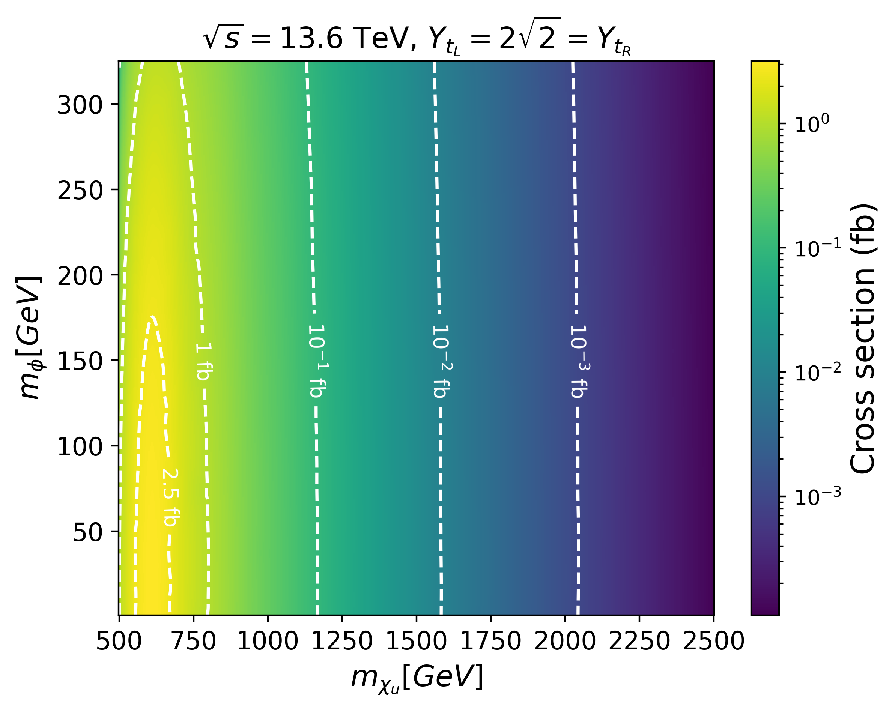
\includegraphics[width=0.85\linewidth]{Images/cross_section_by_masses.pdf}
    \caption{Projected cross section (fb) plot for $pp\to t \chi_\mathrm{u} \phi'$ and subsequent decay as a function of $m(\chi_\mathrm{u})$ and $m(\phi')$.}
    \label{fig:xs-plot}
\end{figure}

\begin{table}[]
  \begin{tabular}{l r}
    \hline
    {Background Process} & {Cross-Section $\sigma$ [\textrm{pb}]} \\
    \hline
   $\mathrm{pp} \to \mathrm{t} \overline{\mathrm{t}} \, \mu^+ \mu^-$ & $2.574\times 10^{-3}$  \\
    $\mathrm{pp} \to \mathrm{b}\overline{\mathrm{b}}\, \mu\mu\mu\nu $ & $4.692 \times 10^{-4}$ \\
    \hline
  \end{tabular}
  \centering
  \caption{A summary of dominant SM backgrounds produced by $\mathrm{pp}$ collisions and their cross sections in pb, as computed by \texttt{MadGraph} with $n = 10^6$ events.}
  \label{tab:dominantbkgs}
\end{table}

\begin{figure}[]
\centering
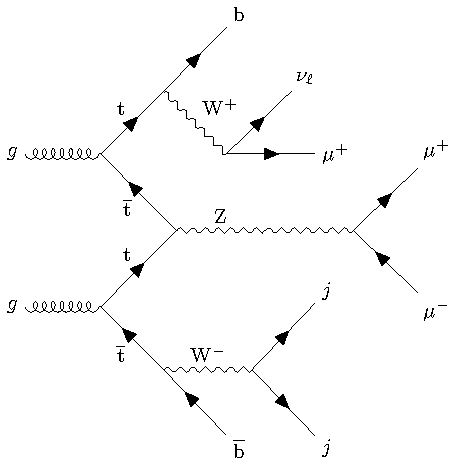
\includegraphics[width=.75\linewidth]{Images/bg_Z_full.pdf}
\caption{Representative Feynman diagram for a background event. A $Z$ boson is produced in association with a top quark through the fusion of a top, anti top pair from incoming protons. The $Z$ boson subsequently decays to a pair of muons and the two spectator top quarks decay semi-leptonically and purely hadronically to muons, neutrinos and jets, resulting in the same final states as the signal event.\label{fig:v}}
\end{figure}

\section{Data Analysis Using Machine Learning}\label{sec:ML}
The analysis of signal and background events is performed utilizing machine learning techniques. A machine learning-based approach offers sizeable advantages when compared to traditional event classification techniques. Unlike conventional methods, machine learning models have the capability to simultaneously consider all kinematic variables, allowing them to efficiently navigate the complex and high-dimensional space of event kinematics. Consequently, machine learning models can effectively enact sophisticated selection criteria that take into account the entirety of this high-dimensional space. This makes them ideal for high-energy physics applications.

The BDT method is a powerful machine learning technique that has proven its effectiveness in various applications, particularly in the field of collider physics. In this method, decision trees are trained greedily in a sequential manner, with each tree focusing on learning the discrepancies or residuals between its predictions and the expected values obtained from the previously trained tree. This iterative process aims to progressively minimize errors, making BDTs a particularly effective approach for enhancing model performance.

In the context of collider physics, BDTs have demonstrated their utility in addressing classification problems. In particular, BDTs can effectively discriminate between signal and background events, enabling accurate and efficient event classification. Their ability to handle subtle non-linear relationships within the data with high interpretability makes BDTs a valuable tool to handle large amounts of data with a large number of parameters for each event. 

The first step in our workflow involves the use of a specialized \texttt{MadAnalysis Expert Mode} C++ script~\parencite{CONTE2013222}. This script extracts essential kinematic and topological information from the simulated samples. The script will process the aforementioned variables contained within these files and transform them into a structured and informative CSV (Comma-Separated Values) format that can be used to train our machine learning models. These kinematic variables include crucial details about the events, such as particle momenta, energies, and topologies, providing the fundamental building blocks for our machine learning analysis. Figure~\ref{fig:feature_importance} shows the features that are used for training the machine learning models and their importance for a benchmark point.

To account for the differential significance of various events, we apply cross-section weighting. This ensures that the relative importance of signal and background events is appropriately balanced in the dataset. This weighting is crucial for addressing the varying likelihood of observing different types of events in high-energy physics experiments. The prepared and weighted datasets are then passed to our \texttt{MadAnalysis Expert Mode} C++ script, where the simulated signal and background events are initially filtered, before being passed to the CSV file for use by the machine learning algorithm. The filtering process requires at least one well-reconstructed and identified $\mathrm{b}$-jet candidate, at least one jet (regular or FJ) not tagged as a $\mathrm{b}$ jet, and exactly three identified muons. The filtering selections are motivated by experimental constraints, such as the geometric constraints of the CMS/ATLAS detectors, the typical kinematic thresholds for the reconstruction of particle objects, and the available lepton triggers which also drive the minimal kinematic thresholds. Selected jets must have $p_{\mathrm{T}} > 30$ $\textrm{GeV}$ and $|\eta(j)| < 5.0$, while $\mathrm{b}$-jet candidates with $p_{\mathrm{T}} > 20$ $\textrm{GeV}$ and $|\eta(\mathrm{b})| < 2.5$ are chosen. The $\mu$ object must pass a $p_{\mathrm{T}} > 35$ $\textrm{GeV}$ threshold and be within a $|\eta(\ell)| < 2.3$. We will refer to this filtering criteria as pre-selections. The efficiency of the pre-selections depends on $m(\phi')$ and $m(\chi_{\mathrm{u}})$, but is typically about 25-30\% for the signal samples. Events passing this pre-selection are used as input for the machine learning algorithm, which classifies them as signal or background, using a probability factor. 

\begin{figure}
\centering
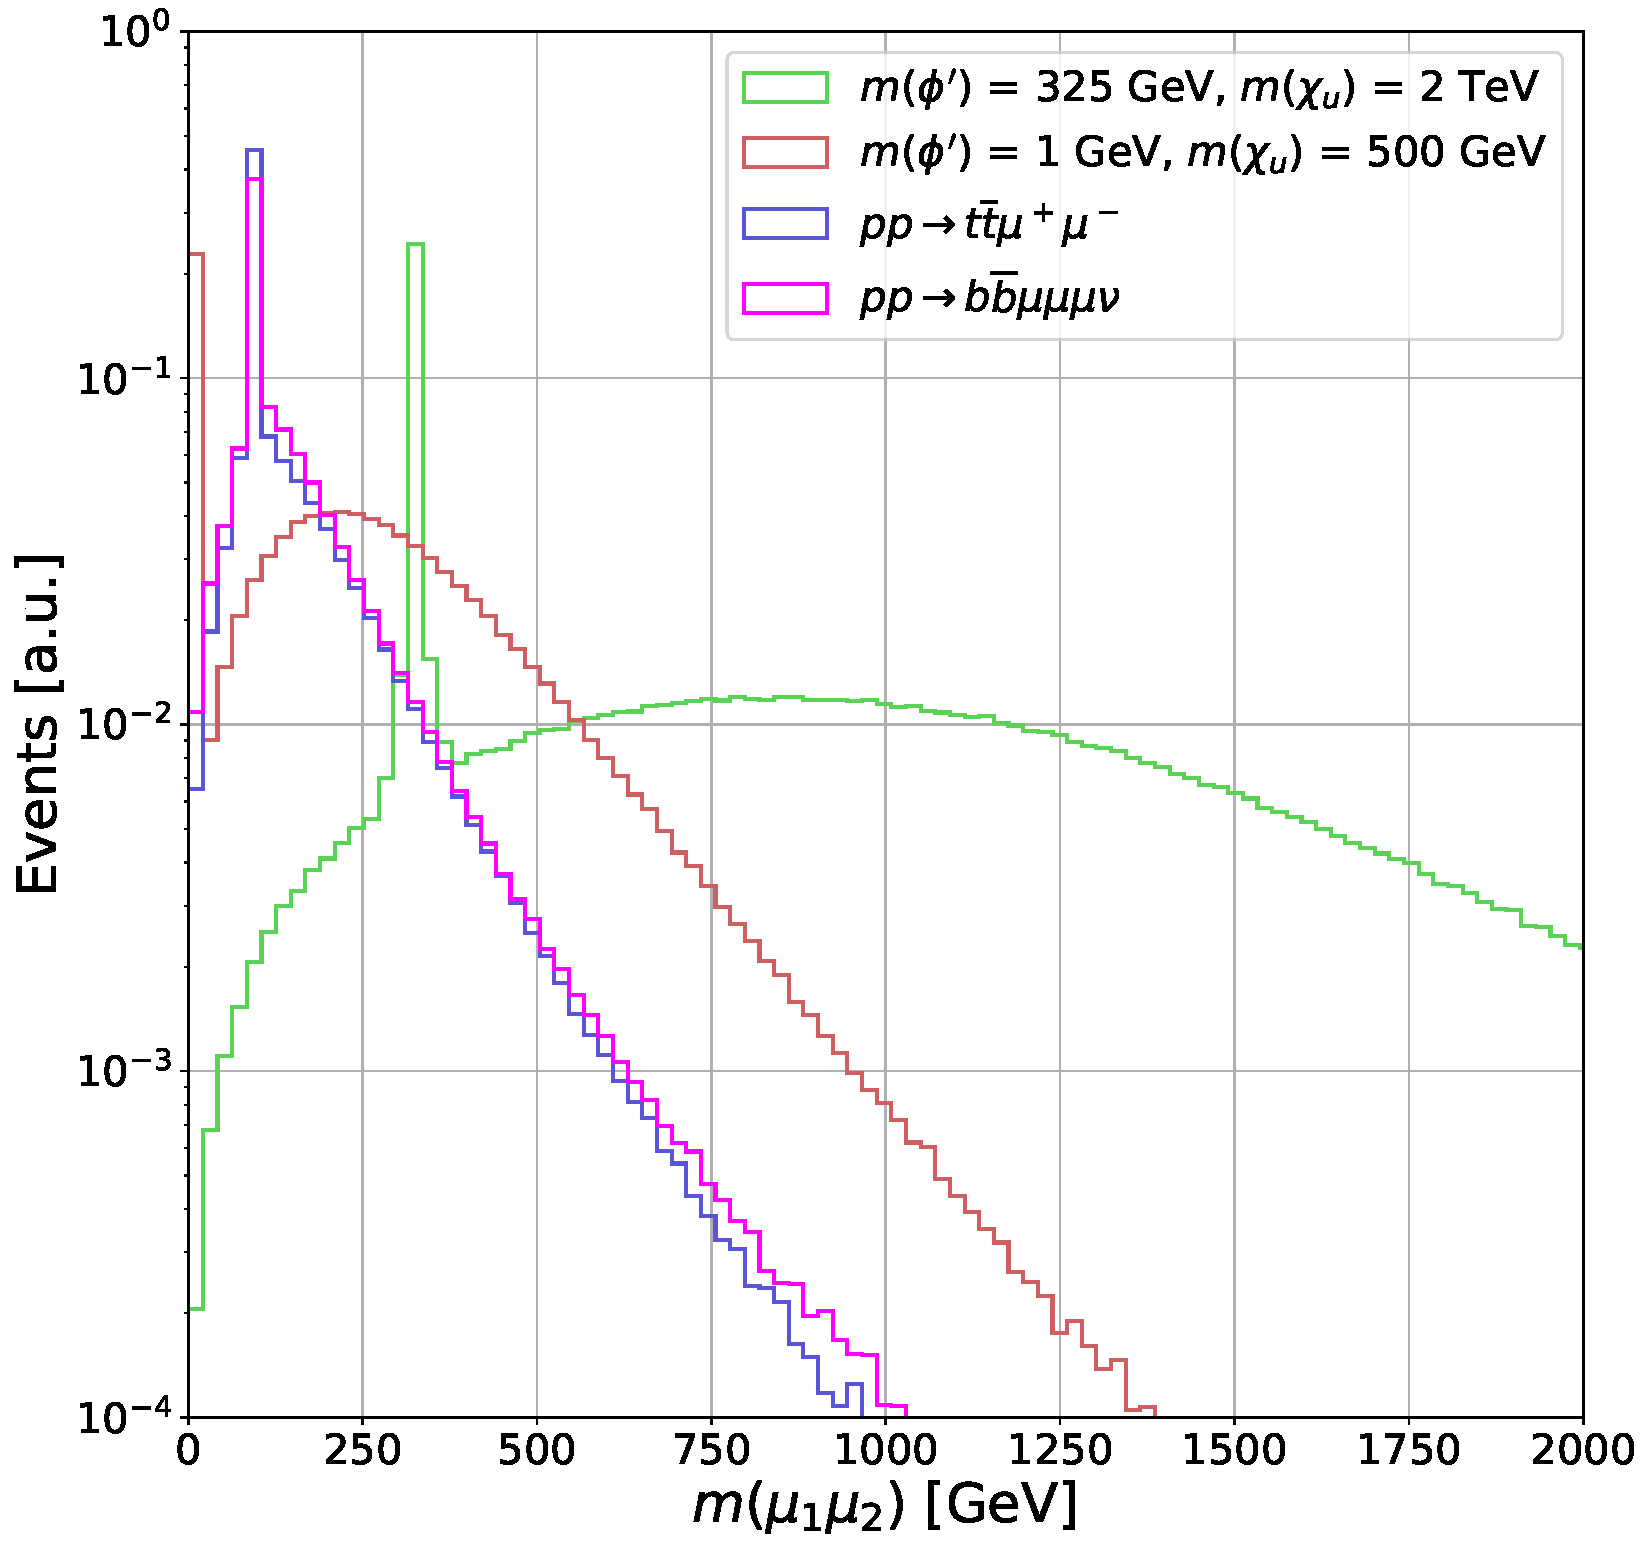
\includegraphics[width=.95\linewidth]{Images/M_mu_1_2.pdf}
\caption{Invariant mass distribution of the muon pair with the highest and second highest transverse momentum. The distributions are shown for the two main SM background processes and two signal benchmark points.\label{fig:_mu12}}
\end{figure}

We explore the performance of a diverse set of machine learning models, specifically three neural networks of differing architectures and a BDT algorithm. To ensure robust model assessment, we employed a standard 90-10 train-test split of the dataset, partitioning it into a 90\% portion for training and a 10\% portion for testing. This division allows us to gauge the generalization capabilities of our models on unseen data.  

The training and evaluation of the BDT were carried out in a high-performance computing environment. Specifically, an Nvidia A100 GPU was used. The canonical \texttt{PyTorch}~\parencite{paszke2019} deep learning framework was employed for configuring, training, and evaluating the neural networks. PyTorch is well-regarded for its flexibility and performance in deep learning applications.

For the BDT algorithm, we used hyperparameters $\eta=0.3$, $\gamma = 0$, and $\texttt{max\_depth} = 6$. The \texttt{XGBoost}~\parencite{chen_xgboost_2016} library was used for the implementation of the Boosted Decision Tree algorithm. It offers high efficiency, optimization, and interpretability, making it a suitable choice for this particular task. 

\begin{figure}
\centering
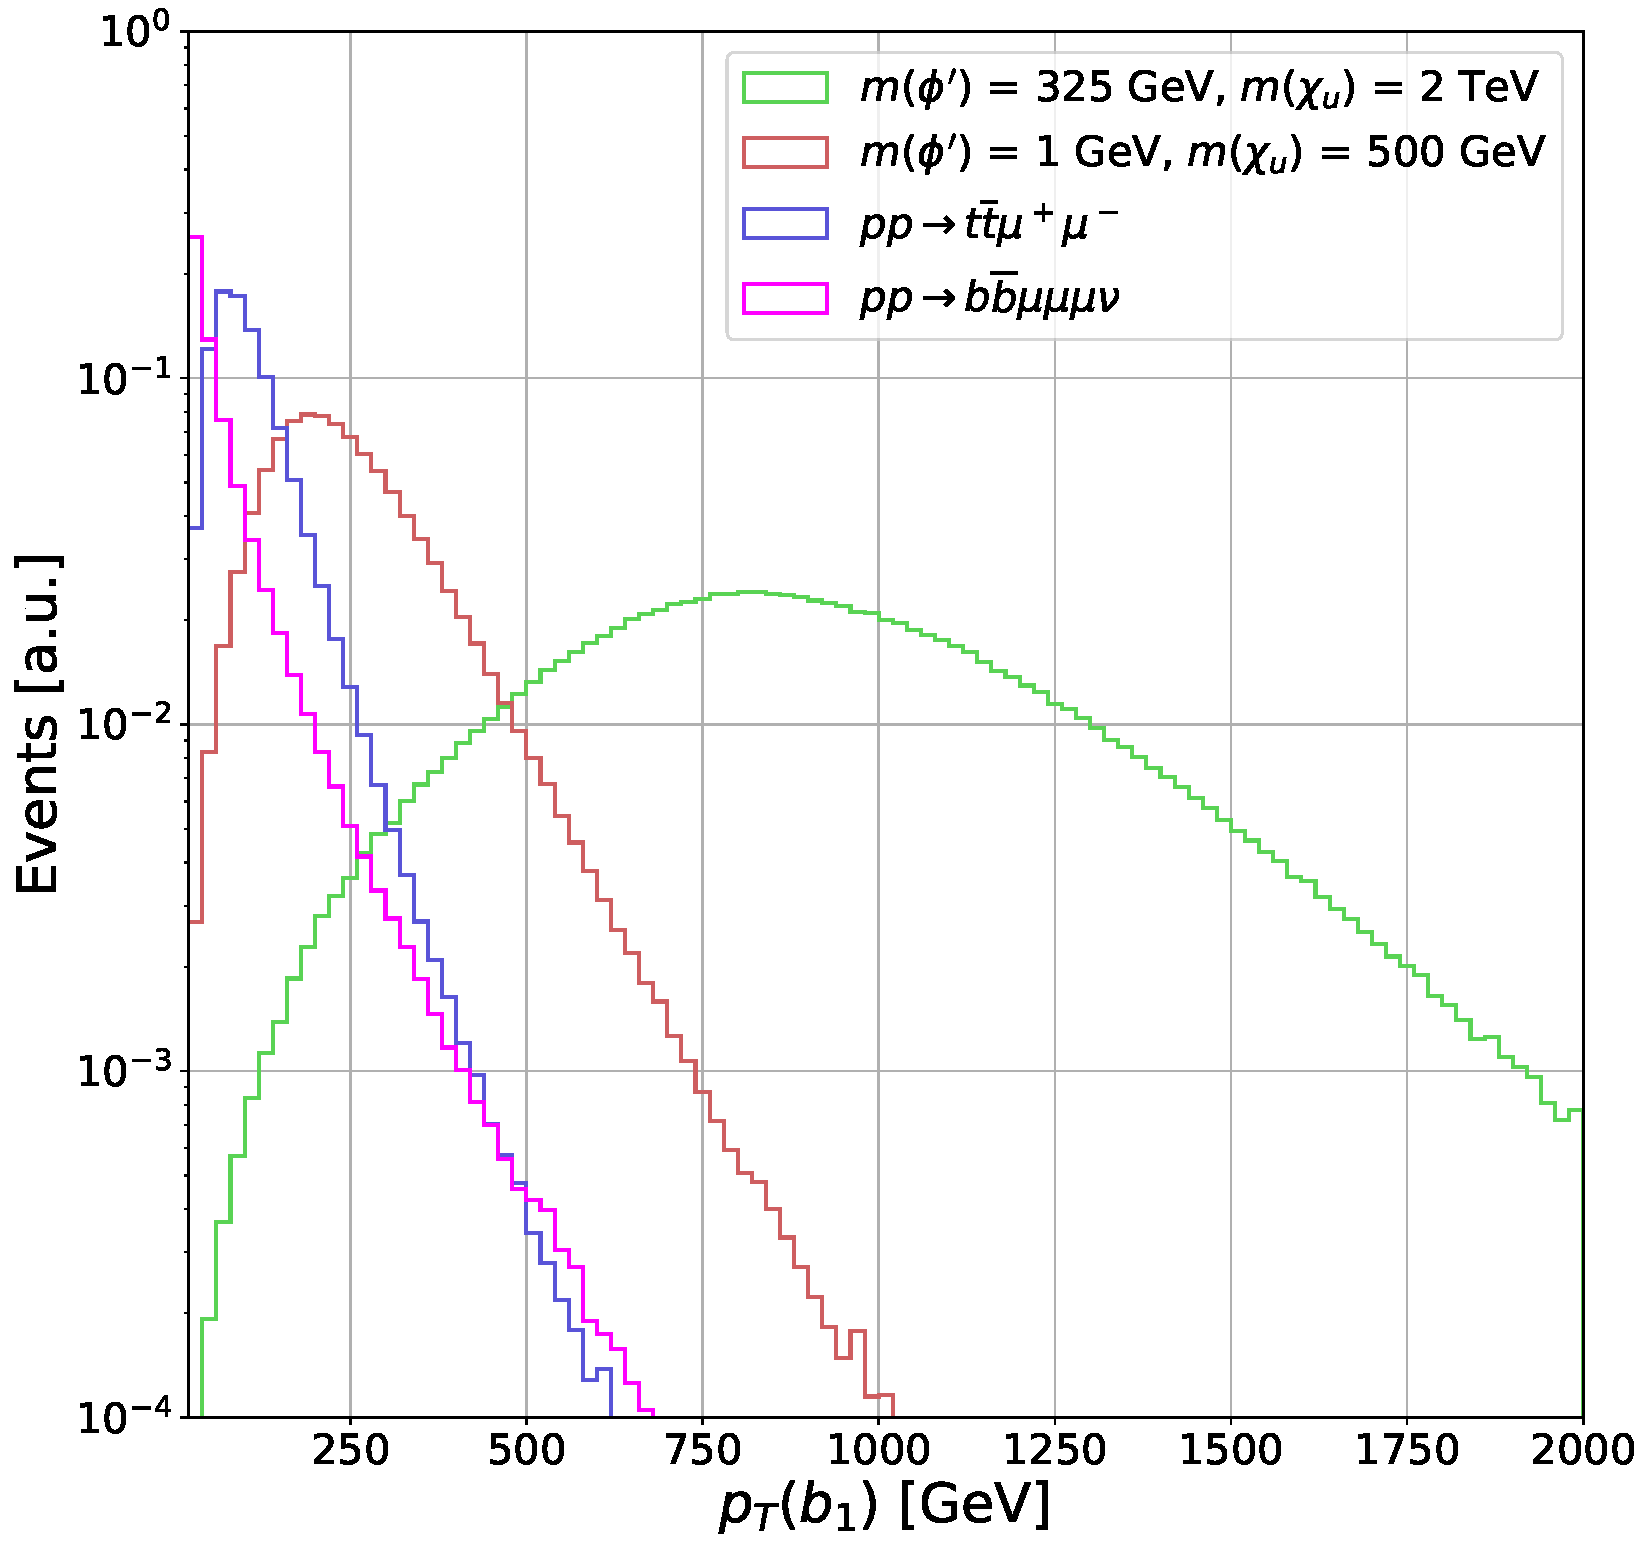
\includegraphics[width=.75\linewidth]{Images/PT_b1.pdf}
\caption{Transverse momentum distribution of the leading \textrm{b}-quark jet candidate. The distributions are shown for the two main SM background processes and two signal benchmark points.\label{fig:pTb1}}
\end{figure}

\begin{figure}
\centering
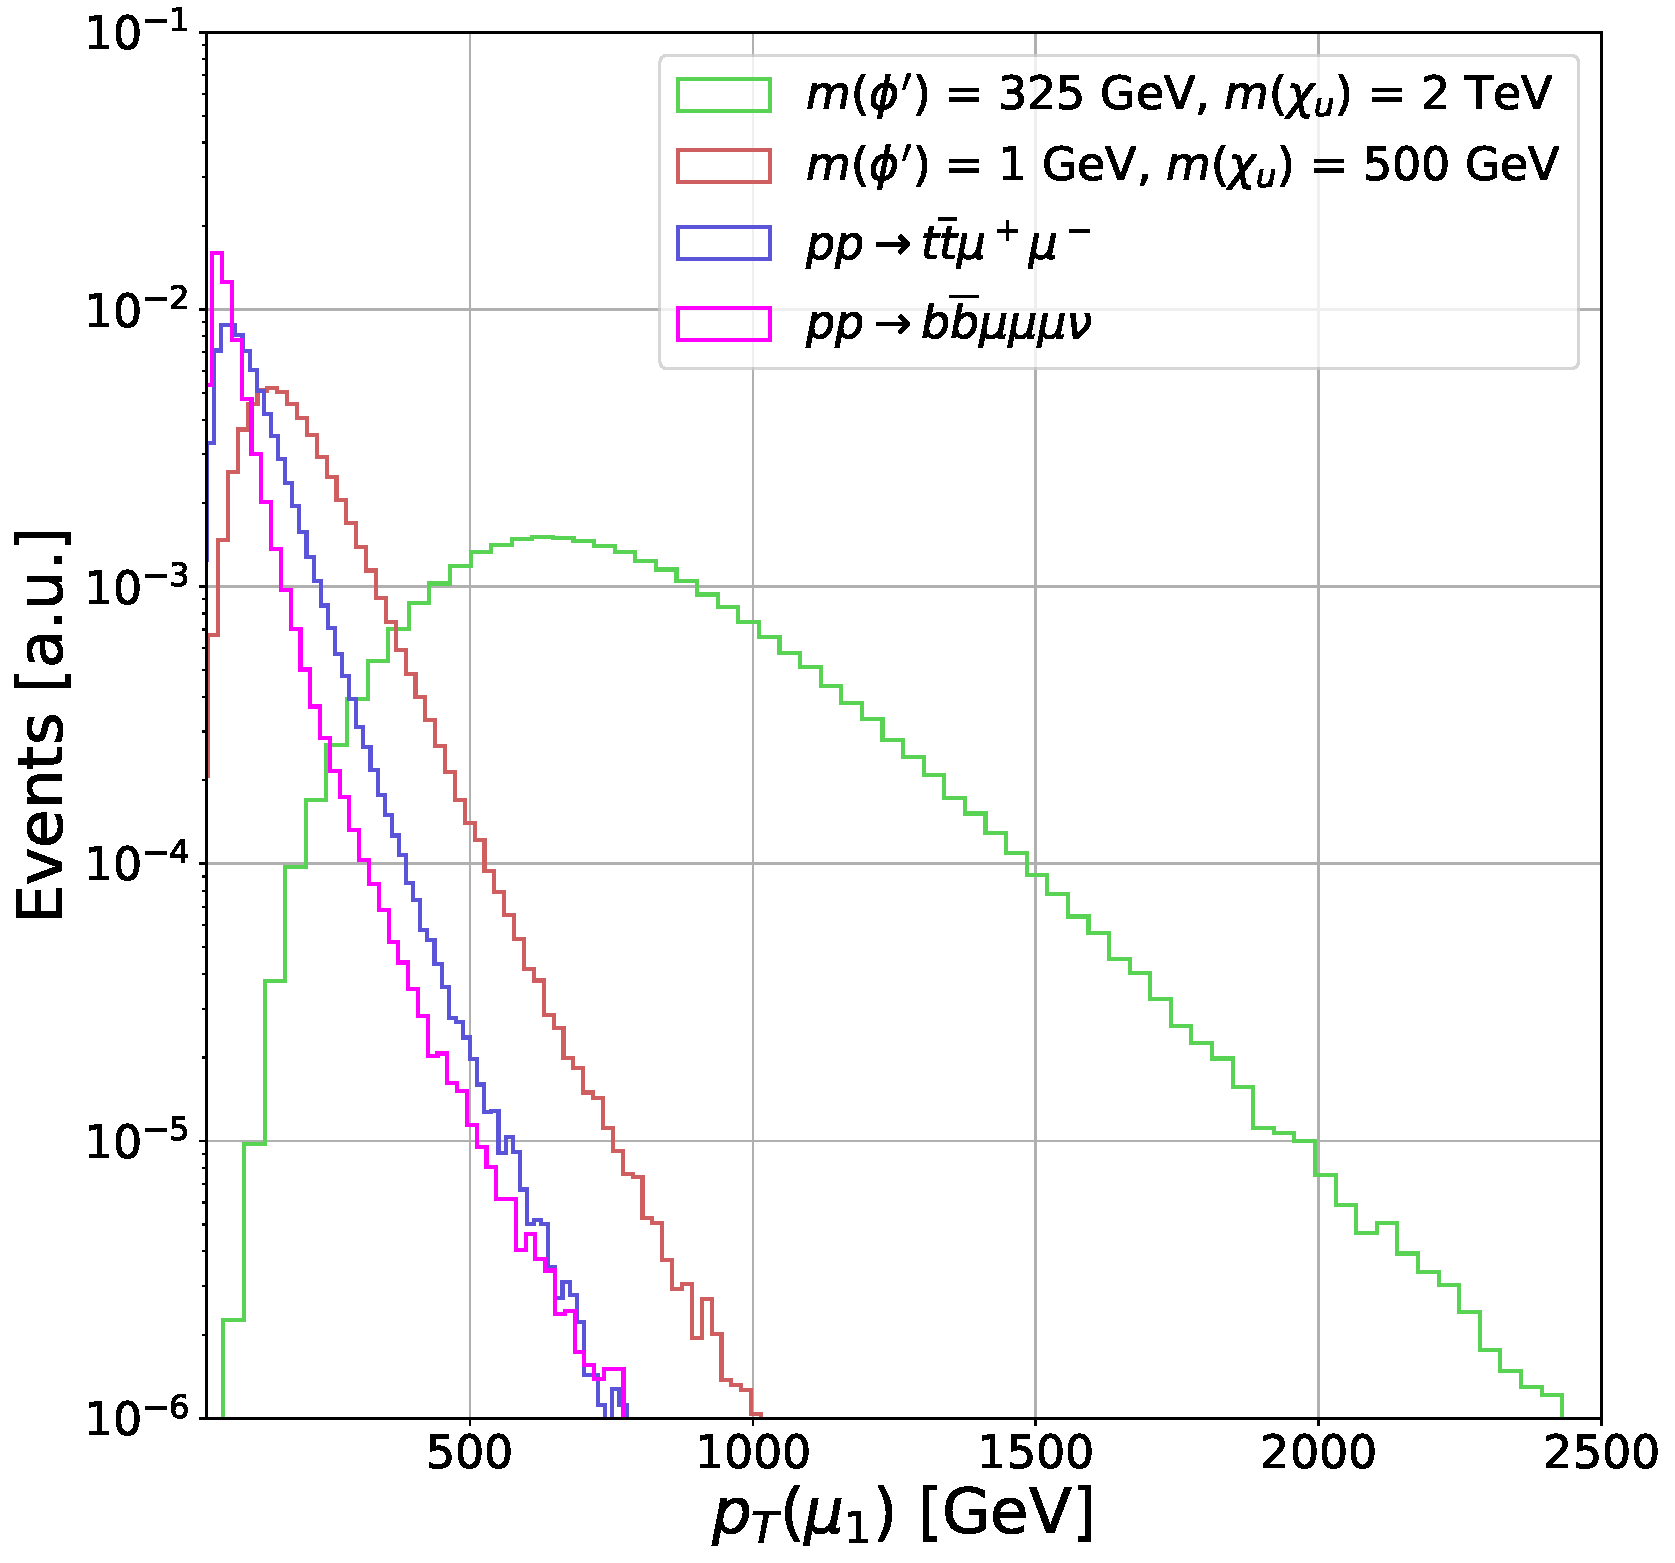
\includegraphics[width=.75\linewidth]{Images/PT_mu1_1.pdf}
\caption{Transverse momentum distribution of the leading muon candidate. The distributions are shown for the two main SM background processes and two signal benchmark points.\label{fig:pTmu1}}
\end{figure}

\begin{table}
    \centering
    \begin{tabular}{c  c  c}
    \hline
    { Model} & { Train/Test Acc. } & { Training Time} \\
    \hline
    \small
    BDT & N.A./0.9993  & 6s\\
    Neural Network 1 & 0.9999/0.9997 & 1h 58m \\
    Neural Network 2 & 0.9999/0.9998 & 2h 12m \\
    Neural Network 3 & 0.9999/0.9998 & 2h 32m\\
    \hline
    \end{tabular}
    \caption{Train/test results for the ML models.}
    \centering
\end{table}

It is worth mentioning that we experimented with deep neural networks of various architectures. Although we found that they yield similar signal sensitivity to the BDT, the complex nature of the studies in this
work (particle objects considered, experimental constraints in a high luminosity LHC, etc.) motivates the use of a BDT over a deep neural network because of its usefulness, efficiency, and simplicity in understanding the machine learning output in addition to significantly shorter training times. Therefore, we perform our proceeding analysis using the BDT. The outcomes of our model training and evaluation are presented in Table 3. 

\section{Results}\label{sec:results}
Figures~\ref{fig:_mu12},~\ref{fig:pTb1}, and~\ref{fig:pTmu1} show relevant kinematic distributions for two benchmark signal points and the dominant SM backgrounds, using the subset of events passing the pre-selections defined above. The signal benchmark points in these figures are $m(\phi^{'}) = 325 \, \mathrm{GeV}$, $m(\chi_{\mathrm{u}}) = 2\, \mathrm{TeV}$, and $m(\phi^{'}) = 1 \, \mathrm{GeV}$, $m(\chi_{\mathrm{u}}) = 500\, \mathrm{GeV}$. The distributions are normalized such that the area under the curve is unity. These distributions correspond to the reconstructed mass, $m(\mu_{1}, \mu_{2})$, between the two muon candidates with the highest transverse momentum ($\mu_{1}$ and $\mu_{2}$), 
the transverse momentum of the b-jet candidate with the highest transverse momentum $p_{\mathrm{T}}$ ($\mathrm{b_{1}}$), and the muon candidate with the highest transverse momentum $p_{\mathrm{T}}$ ($\mu_{1}$), respectively. 
These distributions are among the variables identified by the BDT algorithm with the highest signal to background discrimination power (see Figure~\ref{fig:feature_importance}).

As can be seen from Figure~\ref{fig:_mu12}, the $\phi'$ mass can be reconstructed through its associated muon decay pair, which is observed as a peak in the $m(\mu_{1}, \mu_{2})$ distribution around the expected $m(\phi')$ value, and has low- and high-mass tails which are a consequence of cases where the leading and/or subleading muon is not from the $\phi'$ decay, but rather from the associated $\mathrm{W}$ boson from the $\chi_{\mathrm{u}}$ decay. For the backgrounds, muons come from \textrm{Z} (\textrm{W}) decays. Therefore, the $m(\mu_{1}, \mu_{2})$ background distributions show a peak near $m_{\mathrm{W/Z}}$, combined with a broad distribution indicative of the combination of two muon candidates from different decay vertices. We note that the $\phi'\to\mu^{+}\mu^{-}$ decay width depends on the square of the $\phi'\to\mu^{+}\mu^{-}$ coupling and  $\frac{m_{\mu}^{2}}{m(\phi')^{2}}$ and is thus suppressed by the relatively small muon mass. For the new physics phase space considered in this paper, the $\phi'$ decay width is less than 1\% of the $\phi'$ resonant mass. Furthermore, as indicated previously, the signal/background interference effects are small and negligible compared to effects from experimental resolution. Therefore, the width of the $m(\mu_{1}, \mu_{2})$ signal distributions is driven by the experimental resolution in the reconstruction of the muon momenta, as well as the probability that the two leading muons are the correct pair from the $\phi'$ decay. Since the probability that the two highest-$p_{\mathrm{T}}$ muons are the correct pair from the $\phi'\to\mu^{+}\mu^{-}$ decay depends on $m(\phi')$ and $m(\chi_\mathrm{u})$, it is important to include all possible combinations of dimuon pairs (i.e., $m(\mu_{1}, \mu_{3})$ and $m(\mu_{2}, \mu_{3})$) in the training of the BDT. 

Figure~\ref{fig:pTb1} shows the  distribution for the \textrm{b}-jet candidate with the highest $p_{\mathrm{T}}$, $p_{\mathrm{T}}(\mathrm{b}_1)$, for the same simulated samples shown in Figure~\ref{fig:_mu12}. Based on the signal topology and our choice of parameter space (i.e., $m(\chi_\mathrm{u}) > m_{\mathrm{t}}$), it is expected that the leading $\mathrm{b}$-jet candidate comes from the $\chi_\mathrm{u}$ decay, with an average $p_{\mathrm{T}}$ close to $\frac{m(\chi_\mathrm{u}) - m_{\mathrm{W}}}{2}$, as observed in Figure~\ref{fig:pTb1}. For the $\mathrm{t} \overline{\mathrm{t}} \mu^{+}\mu^{-}$ background, the \textrm{b}-jet candidates come from top-quark decays. Therefore, their average transverse momentum is expected to be $\frac{m_{\mathrm{t}} - m_{\mathrm{W}}}{2} \approx 45$~\textrm{GeV}, as observed in Figure~\ref{fig:pTb1}. On the other hand, the \textrm{b}-jet candidates for the $\mathrm{b} \overline{\mathrm{b}}\mu\mu\mu\nu$ background can come from off-mass-shell $\mathrm{Z}^{*}/\gamma^{*}$, and thus typically have an even softer spectrum in comparison to the $\mathrm{t} \overline{\mathrm{t}} \mu^{+}\mu^{-}$ background.

Figure~\ref{fig:pTmu1} shows the  distribution for the muon candidate with the highest $p_{\mathrm{T}}$, $p_{\mathrm{T}}(\mu_{1})$. Similar to Figure~\ref{fig:pTb1}, when $m(\chi_\mathrm{u}) > m_{\mathrm{t}}$ it is expected that the leading muon candidate comes from the $\chi_\mathrm{u}$ decay, with an average $p_{\mathrm{T}}$ of approximately $\frac{m(\chi_\mathrm{u}) - m_{\mathrm{W}}}{4}$, as observed in Figure~\ref{fig:pTmu1}. For the major SM backgrounds, the muon candidates come from Z/W/$\gamma^{*}$ decays. Therefore, their average transverse momentum is expected to be much lower, $\frac{m_{\mathrm{Z/W}}}{4} \approx 40-45$~\textrm{GeV}. This kinematic feature provides a nice handle to discriminate high $m(\chi_\mathrm{u})$ signal events amongst the large SM backgrounds, which have lower average $p_{\textrm{T}}(\mu)$ constrained by the SM weak boson masses.

In addition to these aforementioned variables in Figures~\ref{fig:_mu12}-\ref{fig:pTmu1}, several other kinematic variables were included as inputs to the BDT algorithm. In particular, 27 such variables were used in total, and these included the momenta of $\mathrm{b}$ and muon candidates; invariant masses of pairs of muons; angular differences between $\mathrm{b}$ jets and between the muons. 

As mentioned above, the variables $m(\mu_{i}, \mu_{j})$ for $i, j \neq 1$ provide some additional discrimination between signal and background when the leading muons are not a $\phi'$ decay candidate. The angular separation variables, such as $\Delta R(\mu_{i}, \mu_{j})$, are designed to be sensitive to lower mass $\phi'$, since the low rest mass of those particles means they acquire more boost, and thus smaller angular separation $\Delta R$ between the muon candidates. The trained BDT returns the discriminating power of each of its inputs, and the feature importance for each variable is shown in Figure~\ref{fig:feature_importance} for a signal benchmark point with $m(\phi')=325\, \mathrm{GeV}$ and $m(\chi_\mathrm{u})=2000\, \mathrm{GeV}$.

\begin{figure}
\centering
  \centering  \includegraphics[width=.75\linewidth]{Images/XGB_output.pdf}
  \caption{Output of the gradient boosting algorithm for a benchmark $m(\phi') = 100$~\textrm{GeV} and $m(\chi_\mathrm{u}) = 500\, \mathrm{GeV}$ signal, and dominant backgrounds. The distributions are normalized to unity.}
  \label{fig:xgboostout}
\end{figure}

Figure~\ref{fig:xgboostout} shows  the distributions for the output of the BDT algorithm, normalized to unity, for the representative signal benchmark point of $m(\phi') = 1\, \mathrm{GeV}$, $m(\chi_\mathrm{u}) = 0.5\, \mathrm{TeV}$ and the two dominant backgrounds. The output of the BDT algorithm is a value between 0 and 1, which quantifies the likelihood that an event is either background-like (BDT output near 1) or signal-like (BDT output near 0). Figure~\ref{fig:ROC} illustrates the true positive rate (TPR), defined as the probability of correctly selecting signal events using the BDT output, plotted against the false positive rate (FPR), defined as the probability of incorrectly selecting background events. For example, for $m(\phi') = 100\, \mathrm{GeV}$ and $m(\chi_\mathrm{u}) = 500\, \mathrm{GeV}$, when signal events are selected at 65\% probability, the background is selected at about $10^{-3}$ probability. We note that the primary discriminating feature between the signal and background is the boosted b-jet $p_T$ coming from the $\chi_u$ vector-like quark. The $p_T$ of said b jet increases with $m(\chi_\mathrm{u})$, peaking at around $[m(\chi_\mathrm{u}) - m(\textrm{W})] / 2$. This enhanced boost increases the separation between signal and background, improving the performance of the BDT algorithm as $m(\chi_\mathrm{u})$ increases. 

\begin{figure}
\centering
  \centering
  \includegraphics[width=.75\linewidth]{Images/ROC_Curve.pdf}
  \caption{Receiver operating characteristic curve of the BDT algorithm for three different signal benchmark scenarios.}
  \label{fig:ROC}
\end{figure}

\begin{figure}
\centering
  \centering
  \includegraphics[width=.75\linewidth]{Images/feature_importance.pdf}
  \caption{Relative importance of features in training for a benchmark signal scenario with $m(\phi')=325\, \mathrm{GeV}$ and $m(\chi_\mathrm{u})=2000\, \mathrm{GeV}$.}
  \label{fig:feature_importance}
\end{figure}

The outputs from the BDT machine learning algorithm are used to perform a profile-bin likelihood analysis to estimate the signal significance for a luminosity of 3000 $\mathrm{fb^{-1}}$, corresponding to the expected amount of collected data by the end of the LHC era. For this purpose, the BDT distributions are normalized to cross section times pre-selection efficiency times luminosity for the different signal models. The significance is then calculated using the expected bin-by-bin yields of the BDT output distribution in a profile likelihood fit, using the ROOTFit~\parencite{Butterworth:2015oua} package developed by CERN. The expected signal significance $Z_\text{sig}$ is calculated using the probability of obtaining the same test statistic for the  signal plus background and the signal-null hypotheses, defined as the local $p$-value. Similar to Refs.~\parencite{Florez:2021zoo, Florez:2019tqr, Florez:2018ojp, Florez:2017xhf, VBFZprimePaper, Florez:2016lwi, Leonardi_2020}, the significance  corresponds to the point where the integral of a Gaussian distribution between $Z_\text{sig}$ and $\infty$ results in a value equal to the local $p$-value. The estimation of $Z_\text{sig}$ incorporates  systematic uncertainties. The uncertainty values have been included as nuisance parameters, considering lognormal priors for normalization and Gaussian priors for uncertainties associated with the modeling of the shapes similar to Refs.~\parencite{natalia2021longtermlhcdiscoveryreach, PhysRevD.103.095001}. 

The systematic uncertainties that have been included result from experimental and theoretical constraints.   A 1-5\% systematic uncertainty, depending on the simulated MC sample, has been included to account for the choice of Parton Distribution Function (PDF) set. The systematic uncertainty effect was incorporated following the PDF4LHC~\parencite{Butterworth:2015oua} recommendations. This systematic uncertainty has a small impact on the expected event yields for signal and background, but it does not affect the shape of the BDT output distribution. We additionally considered theoretical uncertainties related to the absence of higher-order contributions to the signal cross sections, which can change the pre-selection efficiencies and the shapes of kinematic variables used as inputs to the BDT algorithm. This uncertainty was calculated by varying the renormalization and factorization scales by $\times 2$, and studying the resulting change in the bin-by-bin yields of the BDT distributions. They are found to be at most 2\% in a given bin. 
%Additional theoretical uncertainties were taken into account, including the potential impact of higher-order contributions to the signal cross sections. These contributions can influence the pre-selection efficiency and shapes of kinematic distributions utilized by the BDT algorithm. The uncertainty associated with this is determined by adjusting the renormalization and factorization scales by a factor of two relative to the nominal value and considering the complete change in the bin-by-bin yields of the BDT output distribution. The maximum impact of these uncertainties in a given bin is found to be 1-3\%. 

Regarding experimental uncertainties, following experimental measurements from CMS on the estimation of the integrated luminosity, a conservative 3\% effect has been included~\parencite{lumiRef}. A 5\% systematic uncertainty associated with the reconstruction and identification of $\mathrm{b}$-quark jets has been included, independent of $p_\mathrm{T}$ and $\eta$ of the $\mathrm{b}$-jet candidates. According to Ref.~\parencite{CMSbtag}, this uncertainty is correlated between signal and background processes with genuine  \textrm{b}-jets and is also correlated across BDT bins for each process. For muons, we include a 2\% uncertainty associated with the reconstruction, identification, and isolation requirements, and a 3\% systematic uncertainty to account for scale and resolution effects on the momentum and energy measurement. 
%For muon reconstruction, identification, and isolation requirements, there is a 1-2\% uncertainty, while a 1-3\% systematic uncertainty is applied to variations in energy/momentum scale and resolution. 
We consider jet energy scale uncertainties ranging from 2-5\%, contingent on $\eta$ and $p_\mathrm{T}$, resulting in shape-based uncertainties on the BDT output distribution. Jet energy scale uncertainties were assumed to range from 1-5\%, contingent on $\eta$ and $p_\mathrm{T}$. These assumptions lead to shape-based uncertainties on the BDT output distribution, varying from 1-2\%. Additionally, we include  a 10\% systematic uncertainty to account for errors in the signal and background predictions. Considering all the various sources of systematic uncertainties, our conservative  estimate yields a total effect of about 20\%. 

Figure~\ref{fig:/significance_3000} shows the expected signal significance considering an integrated luminosity of 3000 $\mathrm{fb^{-1}}$. The significance is shown as a heat map in a two-dimensional plane for different $\phi'$ and $\chi_{\mathrm{u}}$ masses. The x-axis corresponds to $m(\chi_\mathrm{u})$, the y-axis to $m(\phi')$, and the heat map to log$_{10}(\mathrm{Z}_{sig})$. The white dashed lines are contours of constant signal significances of $1.69 \sigma$,  $3\sigma$ and  $5\sigma$ to represent regions of possible exclusion, evidence of new physics, and discovery, respectively. Under these conditions, $\phi'$ ($\chi_{\mathrm{u}}$) masses ranging from 1 to 325 \textrm{GeV} (500 to 1800 \textrm{GeV}) can be probed. The range for a discovery with $5\sigma$ signal significance varies from $\chi_{\mathrm{u}}$ masses from $m(\chi_{\mathrm{u}}) = 770$-1100 \textrm{GeV}, depending  $m(\phi^{'})$. For large $m(\chi_\mathrm{u})$, the significance is almost independent of $m(\phi')$ because the primary discriminating feature—the boosted $b$-quark originating from $\phi'$—is driven predominantly by the large $m(\chi_\mathrm{u})$, with the kinematic impact of $m(\phi')$ being relatively negligible.


\begin{figure}[]
\centering
  \centering
  \includegraphics[width=.85\linewidth]{Images/significance.pdf}
  \caption{Signal significance for the high luminosity LHC era, considering with 3000  $\mathrm{fb}^{-1}$ of collected data.}
  \label{fig:/significance_3000}
\end{figure}

\section{Discussion}\label{sec:discussion}

The LHC will continue to run with pp collisions at $\sqrt{s} = 13.6$~\textrm{TeV} for the next decade. Given the increase in the integrated luminosity expected from the high-luminosity program, it is important to consider unexplored new physics phase space that diverges from the conventional assumptions made in many BSM theories, and which could have remained hidden in processes that have not yet been thoroughly examined. It is additionally crucial to explore advanced analysis techniques, in particular the use of artificial intelligence algorithms, to enhance the probability of detecting these rare corners where production cross sections are lower and discrimination from SM backgrounds is difficult. 

In this work, we examine a model based on a $U(1)_{T^3_R}$ extension of the SM, which can address various conceptual and experimental issues with the SM, including the mass hierarchy between generations of fermions, the thermal dark matter abundance, and the muon $g - 2$, $R_{(D)}$, and $R_{(D^*)}$ anomalies. This model contains a light scalar boson $\phi'$, with potential masses below the electroweak scale, and~\textrm{TeV}-scale vector-like quarks $\chi_\mathrm{u}$. We consider the scenario where the scalar $\phi'$ has family non-universal fermion couplings and $m(\phi') \ge 1$~\textrm{GeV}, as was suggested in Ref.~\parencite{Dutta2020}, and thus the $\phi^{\prime}$ can primarily decay to a pair of muons. Previous works in Refs.~\parencite{Dutta2023, Banerjee_2016} considered scenarios motivating a search methodology with a merged diphoton system from $\phi' \to \gamma\gamma$ decays. The authors of Ref~\parencite{Dutta2023}, in which $m(\phi') < 1$~\textrm{GeV},  indeed pointed out that if the $\phi'$ is heavier than about 1~\textrm{GeV}, then decays to $\mu^+ \mu^-$ can become the preferable mode for discovery, which is the basis for the work presented in this paper. We further note that the final state topology studied in this paper would represent the most important mode for discovery at $m(\phi') < 2 m_{\mathrm{t}}$ where the $\phi' \to \mathrm{t\bar{t}}$ decay is kinematically forbidden. 

The main result of this paper is that we have shown that the LHC can probe the visible decays of new bosons with masses below the electroweak scale, down to the~\textrm{GeV}-scale, by considering the simultaneous production of heavy QCD-coupled particles, which then decay to the SM particles that contain large momentum values and can be observed in the central regions of the CMS and ATLAS detectors. The boosted system combined with innovative machine learning algorithms allows for the signal extraction above the lower-energy SM background. The LHC search strategy described here can be used to discover the prompt decay of new light particles.  An important conclusion from this paper is that the detection prospects for low-mass particles are enhanced when it is kinematically possible to simultaneously access the heavy degrees of freedom which arise in the UV completion of the low-energy model.  This specific scenario in which the couplings of the light scalars are generationally dependent, with important coupling values to the top quark, is an ideal example which would be difficult to directly probe at low energy beam experiments.

The proposed data analysis represents a competitive alternative 
to complement searches already being conducted at the LHC, allowing us to probe $\phi'$ masses from 1 to 325 \textrm{GeV}, for $m(\chi_{\mathrm{u}})$ values up to almost 2~\textrm{TeV}, at the HL-LHC. Therefore, we strongly encourage the ATLAS and CMS Collaborations to consider the proposed analysis strategy in future new physics searches. 
% \chapter{Discussion and results} %Conclusions

\appendix
% \chapter{The CMS Detector and Physical Observables}
\lipsum
\chapter{Standard Model Simulation}
\lipsum

% \chapter{Principle of maximum likelihood and hypothesis testing}
\lipsum
\chapter{Supervised Learning}
\lipsum

\section{The Classification Problem}
\lipsum

\section{The Regression Problem}
\lipsum
% \chapter{Framework}
\chapter{On the Universal Seesaw Mechanism: A Detailed Analysis}\label{app:universal_seesaw}

The masses of the SM fermions are generated not through direct Yukawa couplings to the Higgs, but via a universal seesaw mechanism by mixing with new vector-like fermions $\chi_f$. The most general gauge-invariant and renormalizable Lagrangian for the quark sector is given by:
\begin{align}
\mathcal{L}_{\text{mass}}^{\text{quark}} \supset & \, \bar{Q}_{L}^{i} (Y_{u L})_{ij} \chi_{u R}^{j} \tilde{H} + \bar{Q}_{L}^{i} (Y_{d L})_{ij} \chi_{d R}^{j} H \nonumber \\
& + \bar{\chi}_{u L}^{i} (Y_{u R})_{ij} u_{R}^{j} \phi^{*} + \bar{\chi}_{d L}^{i} (Y_{d R})_{ij} d_{R}^{j} \phi \nonumber \\
& + \bar{\chi}_{u L}^{i} (m_{\chi u})_{ij} \chi_{u R}^{j} + \bar{\chi}_{d L}^{i} (m_{\chi d})_{ij} \chi_{d R}^{j} + \text{h.c.}, \label{eq:L_Yuk_general_detail}
\end{align}
where $i, j = 1,2,3$ are flavor indices. An entirely analogous set of terms exists for the lepton sector. The Yukawa matrices $Y_{uL}, Y_{dL}, Y_{uR}, Y_{dR}$ and the vector-like mass matrices $m_{\chi u}, m_{\chi d}$ are general complex $3 \times 3$ matrices, making the flavor structure highly non-trivial.

\section{Diagonalization and Field Redefinitions}
To make physical predictions, we must diagonalize these matrices. We express them in terms of their singular value decompositions (i.e., their diagonal forms) and the associated unitary mixing matrices:
\begin{align*}
Y_{u L} &= U_{L L}^{\dagger} Y_{u L}^{d} U_{L R}, & Y_{u R} &= U_{R L}^{\dagger} Y_{u R}^{d} U_{R R}, \\
Y_{d L} &= V_{L L}^{\dagger} Y_{d L}^{d} V_{L R}, & Y_{d R} &= V_{R L}^{\dagger} Y_{d R}^{d} V_{R R}, \\
m_{\chi u} &= W_{u L}^{\dagger} m_{\chi u}^{d} W_{u R}, & m_{\chi d} &= W_{d L}^{\dagger} m_{\chi d}^{d} W_{d R}.
\end{align*}
Here, the matrices $Y^{d}$ and $m^{d}$ are real, diagonal, and non-negative. The unitary matrices $U, V, W$ are not physical by themselves but encode the mixing between flavor states.

We now perform a series of field redefinitions to absorb the maximal number of these unitary matrices into the definitions of the fermion fields. The goal is to make as many mass parameters diagonal as possible. The redefinitions are:
\begin{align*}
Q_L &\to U_{LL} Q_L, & \chi_{uR} &\to W_{uR} \chi_{uR}, & \chi_{uL} &\to W_{uL} \chi_{uL}, & u_R &\to U_{RR} u_R, \\
\chi_{dR} &\to W_{dR} \chi_{dR}, & \chi_{dL} &\to W_{dL} \chi_{dL}, & d_R &\to V_{RR} d_R.
\end{align*}
Applying these transformations to the Lagrangian \eqref{eq:L_Yuk_general_detail} and using the definitions above, we obtain the simplified form:
\begin{align*}
\mathcal{L}_{\text{Yuk}} = & \, \bar{Q}_{L} Y_{u L}^{d} (U_{L R} W_{u R}^{\dagger}) \chi_{u R} \tilde{H} + \bar{Q}_{L} (U_{LL}V_{LL}^\dagger) Y_{d L}^{d} (V_{L R} W_{d R}^{\dagger}) \chi_{d R} H \\
& + \bar{\chi}_{u L} (W_{u L} U_{R L}^{\dagger}) Y_{u R}^{d} u_{R} \phi^{*} + \bar{\chi}_{d L} (W_{d L} V_{R L}^{\dagger}) Y_{d R}^{d} d_{R} \phi \\
& + \bar{\chi}_{u L} m_{\chi u}^{d} \chi_{u R} + \bar{\chi}_{d L} m_{\chi d}^{d} \chi_{d R} + \text{h.c.}
\end{align*}
The matrix $\tilde{V}_{\text{CKM}} \equiv U_{LL}V_{LL}^\dagger$ is identified as the unitary matrix that will yield the observed Cabibbo-Kobayashi-Maskawa (CKM) quark mixing. For simplicity, and to focus on the essential mass generation mechanism, we adopt a \textit{flavor-aligned} scenario. This assumes that all other unitary matrices ($U_{LR}$, $W_{uR}$, $W_{uL}$, $U_{RL}$, etc.) are equal to the identity matrix. This is a strong assumption that minimizes new sources of flavor violation beyond the SM. Under this assumption, the Lagrangian simplifies dramatically to:
\begin{align*}
\mathcal{L}_{\text{Yuk}} = & \, \bar{Q}_{L} Y_{u L}^{d} \chi_{u R} \tilde{H} + \bar{Q}_{L} \tilde{V}_{\text{CKM}} Y_{d L}^{d} \chi_{d R} H \\
& + \bar{\chi}_{u L} Y_{u R}^{d} u_{R} \phi^{*} + \bar{\chi}_{d L} Y_{d R}^{d} d_{R} \phi \\
& + \bar{\chi}_{u L} m_{\chi u}^{d} \chi_{u R} + \bar{\chi}_{d L} m_{\chi d}^{d} \chi_{d R} + \text{h.c.}
\end{align*}
All matrices $Y^{d}$ and $m^{d}$ are now diagonal. The only remaining off-diagonal flavor structure is in $\tilde{V}_{\text{CKM}}$.

\section{Symmetry Breaking and the Mass Matrix}
After the electroweak symmetry breaking ($\langle H \rangle = v_h / \sqrt{2}$) and the $U(1)_{T_R^3}$ breaking ($\langle \phi \rangle = v_\phi / \sqrt{2}$), the mass terms for the up-type quarks (and analogously for down-type and leptons) are generated. For a single generation, the mass terms in the basis $(\bar{u}_L, \bar{\chi}_{u L})$, $(u_R, \chi_{u R})^T$ form a $2 \times 2$ matrix:
\begin{equation}
\mathcal{L}_{\text{mass}} = - \begin{pmatrix} \bar{u}_L & \bar{\chi}_{u L} \end{pmatrix}
\begin{pmatrix}
0 & m_L \\
m_R & m_{\chi}
\end{pmatrix}
\begin{pmatrix} u_R \\ \chi_{u R} \end{pmatrix} + \text{h.c.}, \label{eq:mass_matrix_detail}
\end{equation}
where the Dirac masses are:
\begin{align*}
m_L &= \frac{v_h}{\sqrt{2}} Y_{uL}, \\
m_R &= \frac{v_\phi}{\sqrt{2}} Y_{uR}.
\end{align*}
The entry $m_{\chi}$ is the vector-like mass. For three generations, this generalizes to a $6 \times 6$ matrix:
\begin{equation}
M_f = \begin{pmatrix}
0 & m_L \\
m_R & m_{\chi}
\end{pmatrix},
\end{equation}
where each entry is now a $3 \times 3$ matrix: $m_L = \frac{v_h}{\sqrt{2}} Y_{fL}^{d}$, $m_R = \frac{v_\phi}{\sqrt{2}} Y_{fR}^{d}$, and $m_{\chi} = m_{\chi f}^{d}$.

\section{Bi-Unitary Transformation and Mass Eigenvalues}
The general mass matrix $M_f$ is diagonalized by a bi-unitary transformation:
\begin{equation}
U_{R}^{\dagger} M_f U_{L} = M_f^d = \text{diag}(m_{f_1}, m_{f_2}, m_{f_3}, m_{F_1}, m_{F_2}, m_{F_3}), \label{eq:bi_unitary_detail}
\end{equation}
where $U_{L}$ and $U_{R}$ are $6 \times 6$ unitary matrices. The physical masses are found by solving the eigenvalues of the Hermitian matrices $H_L = M_f M_f^\dagger$ and $H_R = M_f^\dagger M_f$, as $U_L$ diagonalizes $H_L$ and $U_R$ diagonalizes $H_R$.

For the one-generation case, these matrices are:
\begin{align*}
H_L &= M_f M_f^\dagger = \begin{pmatrix}
m_L m_L^\dagger & m_L m_{\chi}^\dagger \\
m_{\chi} m_L^\dagger & m_R m_R^\dagger + m_{\chi} m_{\chi}^\dagger
\end{pmatrix} = \begin{pmatrix}
|m_L|^2 & m_L m_{\chi}^* \\
m_{\chi} m_L^* & |m_R|^2 + |m_{\chi}|^2
\end{pmatrix}, \\
H_R &= M_f^\dagger M_f = \begin{pmatrix}
m_R m_R^\dagger & m_R m_{\chi}^\dagger \\
m_{\chi} m_R^\dagger & m_L m_L^\dagger + m_{\chi} m_{\chi}^\dagger
\end{pmatrix} = \begin{pmatrix}
|m_R|^2 & m_R m_{\chi}^* \\
m_{\chi} m_R^* & |m_L|^2 + |m_{\chi}|^2
\end{pmatrix}.
\end{align*}
The eigenvalues $\lambda$ of $H_L$ (and $H_R$) are found from the characteristic equation $\det(H_L - \lambda \mathbb{I}) = 0$:
\begin{align*}
&\left||m_L|^2 - \lambda \right| \left| |m_R|^2 + |m_{\chi}|^2 - \lambda \right| - |m_L|^2 |m_{\chi}|^2 = 0 \\
&\Rightarrow \lambda^2 - \lambda (|m_L|^2 + |m_R|^2 + |m_{\chi}|^2) + |m_L|^2 |m_R|^2 = 0.
\end{align*}
The solutions to this quadratic equation are the squared masses of the two mass eigenstates:
\begin{align}
m_f^2 &= \frac{1}{2} \left( m_{\chi}^2 + m_L^2 + m_R^2 - \sqrt{ (m_{\chi}^2 + m_L^2 + m_R^2)^2 - 4 m_L^2 m_R^2 } \right), \label{eq:m_f_detail} \\
m_F^2 &= \frac{1}{2} \left( m_{\chi}^2 + m_L^2 + m_R^2 + \sqrt{ (m_{\chi}^2 + m_L^2 + m_R^2)^2 - 4 m_L^2 m_R^2 } \right), \label{eq:m_F_detail}
\end{align}
where we have now assumed all parameters are real for clarity. $m_f$ is the light SM-like fermion mass, and $m_F$ is the heavy vector-like partner mass.

\section{Yukawa Coupling Enhancement and Perturbativity}
Equation \eqref{eq:m_f_detail} is fundamental. It shows that the light mass $m_f$ is not simply proportional to $m_L$ (the SM Higgs VEV). We can solve Eq. \eqref{eq:m_f_detail} for $m_L^2$:
\begin{align*}
m_f^2 (m_{\chi}^2 + m_L^2 + m_R^2 - m_f^2) &= m_L^2 m_R^2 \quad \text{(from the exact seesaw relation)} \\
m_L^2 (m_R^2 - m_f^2) &= m_f^2 (m_{\chi}^2 + m_R^2 - m_f^2) \\
m_L^2 &= m_f^2 \left( \frac{m_{\chi}^2 + m_R^2 - m_f^2}{m_R^2 - m_f^2} \right) = m_f^2 \left( 1 + \frac{m_{\chi}^2}{m_R^2 - m_f^2} \right). \label{eq:m_L_solution_detail}
\end{align*}
Expressing this in terms of the original Yukawa couplings, where $m_L = \frac{v_h}{\sqrt{2}} Y_{fL}$ and the SM Yukawa is defined by $m_f = \frac{v_h}{\sqrt{2}} Y_f^{\text{SM}}$, we find:
\begin{equation}
Y_{fL}^2 = (Y_f^{\text{SM}})^2 \left( 1 + \frac{m_{\chi}^2}{m_R^2 - m_f^2} \right). \label{eq:Y_L_enhanced_detail}
\end{equation}
This relation reveals the core of the universal seesaw mechanism: the Yukawa coupling $Y_{fL}$ that couples the SM fermions to the Higgs is \textit{enhanced} compared to the standard model value $Y_f^{\text{SM}}$. The enhancement factor is $\sqrt{1 + m_{\chi}^2/(m_R^2 - m_f^2)}$.

This has profound implications:
\begin{itemize}
    \item \textbf{Light Fermions (e.g., electron, u-quark):} Here, $Y_f^{\text{SM}} \ll 1$. A large hierarchy $m_{\chi}^2 \gg m_R^2 \gg m_f^2$ can generate this tiny mass from a more ``natural'' $Y_{fL} \sim \mathcal{O}(0.1-1)$.
    \item \textbf{Top Quark:} Here, $Y_t^{\text{SM}} \approx 1$ is already large. An enhancement could easily push $Y_{tL}$ into the non-perturbative regime ($Y_{tL}^2 / 4\pi > 1$). To avoid this, we must require the enhancement factor to be $\mathcal{O}(1)$, which implies $m_{\chi}^2 \lesssim m_R^2 - m_t^2$. Since $m_R = \frac{v_\phi}{\sqrt{2}} Y_{fR}$, this suggests $v_\phi > m_{\chi}$ is a natural condition.
\end{itemize}

\section{Exact Diagonalization and Mixing Angles}
The bi-unitary transformation \eqref{eq:bi_unitary_detail} is performed by matrices that can be parameterized by a mixing angle. For one generation, the left-handed mixing matrix is:
\begin{equation}
U_L = \begin{pmatrix}
\cos\theta_L & \sin\theta_L \\
-\sin\theta_L & \cos\theta_L
\end{pmatrix}.
\end{equation}
The angle $\theta_L$ quantifies the mixing between the SM fermion and its vector-like partner. The exact expressions for the fundamental parameters $m_L, m_R, m_\chi$ in terms of the physical masses $m_f, m_F$ and the mixing angle $\theta_L$ can be found by equating $U_L^\dagger H_L U_L = \text{diag}(m_f^2, m_F^2)$. This yields the system of equations:
\begin{align*}
m_L^2 &= m_f^2 \cos^2\theta_L + m_F^2 \sin^2\theta_L, \\
m_R^2 + m_\chi^2 &= m_f^2 \sin^2\theta_L + m_F^2 \cos^2\theta_L, \\
m_L m_\chi &= (m_F^2 - m_f^2) \sin\theta_L \cos\theta_L.
\end{align*}
Solving this system (and a similar one from $H_R$ for $\theta_R$) gives:
\begin{align}
m_L^2 &= \frac{1}{2} \left( m_f^2 + m_F^2 - (m_F^2 - m_f^2) \cos 2\theta_L \right), \label{eq:m_L_exact_detail} \\
m_R^2 &= \frac{m_f^2 m_F^2}{m_L^2} = \frac{2 m_f^2 m_F^2}{m_f^2 + m_F^2 - (m_F^2 - m_f^2) \cos 2\theta_L}, \label{eq:m_R_exact_detail} \\
m_{\chi}^2 &= m_R^2 + m_F^2 + m_f^2 - m_L^2 - \frac{m_f^2 m_F^2}{m_L^2} = \frac{(m_F^2 - m_f^2)^2 \sin^2 2\theta_L}{4 m_L^2}. \label{eq:m_chi_exact_detail}
\end{align}
Substituting Eq. \eqref{eq:m_L_exact_detail} into the expression for $m_{\chi}^2$ yields the form shown in the original text.

The critical constraint to keep the top Yukawa perturbative is $m_{\chi}^2 < m_R^2$. Using Eqs. \eqref{eq:m_R_exact_detail} and \eqref{eq:m_chi_exact_detail}, the ratio is:
\begin{equation}
\frac{m_{\chi}^2}{m_R^2} = \frac{(m_F^2 - m_f^2)^2 \sin^2 2\theta_L}{4 m_f^2 m_F^2} < 1. \label{eq:constraint_detail}
\end{equation}
For the top quark with $m_f = m_t \approx 173$ GeV and assuming a heavy partner $m_F \gg m_t$, this simplifies to:
\begin{equation}
\frac{m_F^4 \sin^2 2\theta_L}{4 m_t^2 m_F^2} \approx \frac{m_F^2}{4 m_t^2} \sin^2 2\theta_L < 1 \quad \Rightarrow \quad \sin^2 2\theta_L < \frac{4 m_t^2}{m_F^2}. \label{eq:sin_constraint_detail}
\end{equation}
This is a very strong constraint. For example, if $m_F = 1$ TeV, then $\sin^2 2\theta_L < 0.12$, meaning $\theta_L < 10^\circ$. In the small $\theta_L$ limit, $\cos 2\theta_L \approx 1 - 2\theta_L^2$ and $\sin^2 2\theta_L \approx 4\theta_L^2$. Substituting this into Eq. \eqref{eq:m_L_exact_detail}:
\begin{align*}
m_L^2 &\approx \frac{1}{2} \left( m_t^2 + m_F^2 - (m_F^2 - m_t^2)(1 - 2\theta_L^2) \right) \\
&= \frac{1}{2} \left( m_t^2 + m_F^2 - m_F^2 + m_t^2 + 2(m_F^2 - m_t^2)\theta_L^2 \right) \\
&= \frac{1}{2} \left( 2m_t^2 + 2(m_F^2 - m_t^2)\theta_L^2 \right) = m_t^2 + (m_F^2 - m_t^2)\theta_L^2.
\end{align*}
From the constraint \eqref{eq:sin_constraint_detail}, $\theta_L^2 < m_t^2 / m_F^2$. Therefore:
\begin{equation}
m_L^2 < m_t^2 + (m_F^2 - m_t^2) \frac{m_t^2}{m_F^2} = m_t^2 + m_t^2 - \frac{m_t^4}{m_F^2} = 2m_t^2 - \frac{m_t^4}{m_F^2}.
\end{equation}
Converting back to Yukawa couplings:
\begin{equation}
Y_{tL}^2 \lesssim (Y_t^{\text{SM}})^2 \left( 2 - \frac{m_t^2}{m_F^2} \right). \label{eq:Y_final_detail}
\end{equation}
This shows that the maximum enhancement for the top Yukawa is less than a factor of $\sqrt{2}$, which is perfectly perturbative.

The generalization to three generations involves the diagonalization of the full $6 \times 6$ matrices. The matrix $\tilde{V}_{\text{CKM}}$ introduced during field redefinition will manifest in the charged current weak interactions of the mass eigenstates. After diagonalization, the SM $W$ boson will couple not only to the three light quarks but also to the heavy vector-like quarks, with couplings suppressed by the mixing angles $\theta_L^i$. The observed $3 \times 3$ CKM matrix emerges as the effective mixing matrix among the three light quarks when the heavy states are integrated out.

The lepton sector follows an identical procedure for the charged leptons. The neutrino sector, however, offers further richness. The right-handed neutrinos $\nu_R$ can possess both Dirac masses ($m_R$) from coupling to $\phi$ and Majorana mass terms $M_R \bar{\nu}_R^c \nu_R$, which are allowed by the gauge symmetry. The vector-like neutrinos $\chi_\nu$ can also have Majorana masses. This combination of Dirac and Majorana masses for both $\nu_R$ and $\chi_\nu$ can generate a double or triple seesaw mechanism, providing a natural explanation for the tiny masses of the observed light neutrinos. The diagonalization of this extended neutrino mass matrix also generates the Pontecorvo-Maki-Nakagawa-Sakata (PMNS) mixing matrix.

% \chapter{The Two Higgs Doublet Model}
\lipsum
\chapter{The $4321$ Model}
\label{sec:4321}
%%%%%%%%%%%%%%%%%%%%%%%%%%%%%%%%%%%%%%%%%%%%

This appendix summarises the main features of the 4321 model presented in \cite{DiLuzio:2017vat}, based on the construction showed in \cite{DiLuzio2018}. The model is built upon the extended gauge group
\[
\mathcal{G}_{\rm 4321} \equiv SU(4) \times SU(3)' \times SU(2)_L \times U(1)'.
\]
The Standard Model (SM) gauge group, $\mathcal{G}_{\rm 321} \equiv SU(3)_c \times SU(2)_L \times U(1)_Y$, is embedded into $\mathcal{G}_{\rm 4321}$ through two key identifications.

First, the SM strong force is identified with the diagonal subgroup of the two $SU(3)$ factors:
\begin{equation}
SU(3)_c = \left( SU(3)_{[4]} \times SU(3)' \right)_{\rm diag},
\end{equation}
where $SU(3)_{[4]} \subset SU(4)$. Second, and more crucially, the SM hypercharge is a linear combination of charges from the $SU(4)$ and $U(1)'$ sectors:
\begin{equation}
Y = Q_{B-L} + Y'.
\end{equation}
Here, the baryon minus lepton number ($Q_{B-L}$) is generated by a diagonal $SU(4)$ generator, $Q_{B-L} = 2\sqrt{6} T^{15}/3$, 

\marginpar{
As we see in chapter~\ref{ch:U1T3R}, the $U(1)'$ charge could be identified with twice the third component of right-handed isospin, $Y' \equiv 2Q_{T^3_R}$. This specific embedding reveals the model's left-right symmetric foundation; the SM electric charge operator can now be expressed in the manifestly left-right symmetric form:
\begin{equation*}
Q = Q_{T^3_L} + Q_{T^3_R} + \frac{1}{2}Q_{B-L}.
\end{equation*}
}

The spontaneous breaking of the full $\mathcal{G}_{\rm 4321}$ symmetry down to the SM $\mathcal{G}_{\rm 321}$ gives mass to the gauge bosons associated with the broken generators. The spectrum of these new massive vectors and their quantum numbers under the SM group are:
\begin{itemize}
    \item A vector leptoquark, $U \sim (\mathbf{3},\mathbf{1},2/3)$,
    \item A coloron, $g' \sim (\mathbf{8},\mathbf{1},0)$,
    \item A massive neutral boson, $Z' \sim (\mathbf{1},\mathbf{1},0)$.
\end{itemize}
Heuristically, each of these bosons originates from a distinct part of the symmetry breaking pattern: the leptoquark ($U$) emerges from the breaking $SU(4)\to SU(3)_{[4]}\times U(1)_{B-L}$, the coloron ($g'$) from $SU(3)_{[4]}\times SU(3)'\to SU(3)_c$, and the $Z'$ from $U(1)_{B-L}\times U(1)_{T_R^3}\to U(1)_Y$.
% \section{Scalar Sector and Symmetry Breaking}

The spontaneous breaking of the $\mathcal{G}_{\rm 4321}$ symmetry down to the Standard Model $\mathcal{G}_{\rm 321}$ and subsequently to electromagnetism is achieved through a scalar sector comprising four multiplets. The primary breaking $\mathcal{G}_{\rm 4321} \to \mathcal{G}_{\rm 321}$ is induced by the vacuum expectation values (vevs) of three scalar fields:
\begin{itemize}
    \item $\Omega_1 \sim \left( \mathbf{\bar 4}, \mathbf{1}, \mathbf{1}, -1/2 \right)$,
    \item $\Omega_3 \sim \left( \mathbf{\bar 4}, \mathbf{3}, \mathbf{1}, 1/6 \right)$,
    \item $\Omega_{15} \sim \left( \mathbf{15}, \mathbf{1}, \mathbf{1}, 0 \right)$ (taken to be a real field).
\end{itemize}
The final electroweak symmetry breaking, $\mathcal{G}_{\rm 321} \to U(1)_{\rm EM}$, is triggered by the Higgs doublet $H \sim (\mathbf{1},\mathbf{1},\mathbf{2},1/2)$.

A suitable scalar potential (analysed in detail in Section~\ref{scalpot}) allows for a vev configuration that ensures this breaking pattern. Phenomenological constraints suggest a clear hierarchy between these scales:
\begin{equation}
    \langle \Omega_{3} \rangle > \langle \Omega_{1} \rangle \gg \langle \Omega_{15} \rangle \gg \langle H \rangle.
\end{equation}
Given this hierarchy, we simplify the analysis by first considering the $\Omega_{3}$ and $\Omega_{1}$ system in isolation to understand the primary TeV-scale breaking. The effects of incorporating the smaller vevs of $\Omega_{15}$ and $H$ will be discussed subsequently.

To analyze the $\Omega_3$--$\Omega_1$ subsystem, we represent these fields as a $4 \times 3$ matrix and a $4$-vector, transforming as $\Omega_3 \to U^*_4 \Omega_3 U_{3'}^T$ and $\Omega_1 \to U^*_4 \Omega_1$ under $SU(4) \times SU(3)'$, respectively. The desired vacuum configuration that breaks $\mathcal{G}_{\rm 4321}$ to $\mathcal{G}_{\rm 321}$ is:
\begin{equation}
\label{vevconf}
\langle \Omega_3 \rangle = 
\tfrac{1}{\sqrt{2}}
\left(
\begin{array}{ccc}
v_3 & 0 & 0 \\
0 & v_3 & 0 \\ 
0 & 0 & v_3 \\
0 & 0 & 0
\end{array}
\right) \, , \qquad
\langle \Omega_1 \rangle = 
\tfrac{1}{\sqrt{2}}
\left(
\begin{array}{c}
0 \\ 
0 \\ 
0 \\
v_1
\end{array}
\right).
\end{equation}
The most general renormalizable scalar potential that admits this vacuum as a stationary point, and in the limit where the bare masses vanish ($\mu_3 = \mu_1 = 0$) and the cubic coupling is absent ($\lambda_6 = 0$), can be written as:
{\small
\begin{equation}\label{eqscalpot}
\begin{aligned}
V_{\Omega_{3},\Omega_{1}}
= & \mu_1^2 \abs{\Omega_1}^2 + \mu_3^2 \, \Tr (\Omega_3^\dag \Omega_3) 
\\&+ \lambda_1 \left( \Tr (\Omega_3^\dag \Omega_3) - \tfrac{3}{2} v_3^2 \right)^2 
+ \lambda_2 \Tr \left( \Omega_3^\dag \Omega_3 - \tfrac{1}{2} v_3^2 \mathbb{1}_3 \right)^2 \\
& 
+\lambda_3 \left( \abs{\Omega_1}^2 - \tfrac{1}{2} v_1^2 \right)^2 
+ \lambda_4 \left( \Tr (\Omega_3^\dag \Omega_3) - \tfrac{3}{2} v_3^2 \right) \left( \abs{\Omega_1}^2 - \tfrac{1}{2} v_1^2 \right)  \\
& + \lambda_5 \Omega_1^\dag \Omega_3 \Omega_3^\dag \Omega_1 + \lambda_6 \left( \left[ \Omega_3 \Omega_3 \Omega_3 \Omega_1 \right]_1 + \text{h.c.} \right).
\end{aligned}  
\end{equation}
}

\noindent
Here, $\mathbb{1}_3$ denotes the $3\times 3$ identity matrix. We have used a relative rephasing between the fields $\Omega_{1}$ and $\Omega_{3}$ to remove the phase of $\lambda_6$. The unique quartic term,
\begin{equation}
  \left[ \Omega_3 \Omega_3 \Omega_3 \Omega_1 \right]_1 \equiv 
\epsilon_{\alpha\beta\gamma\delta} \epsilon^{abc} (\Omega_3)^\alpha_a (\Omega_3)^\beta_b (\Omega_3)^\gamma_c (\Omega_1)^\delta,
\end{equation}
is required to avoid accidental global symmetries in the scalar potential that would lead to unwanted massless Goldstone bosons.

The inclusion of the other two representations, $\Omega_{15}$ and $H$, in the scalar potential can be safely considered as a perturbation. They are assumed to take the vevs $\langle \Omega_{15} \rangle = T_{15} v_{15}$ and $\langle H \rangle = \tfrac{1}{\sqrt{2}} (0, v)^T$, with $v = 246$ GeV. This treatment is justified because their vevs are subleading for phenomenological reasons and they do not alter the pattern of global symmetries of the $\Omega_3$--$\Omega_1$ potential.
Finally, the decomposition of $\Omega_{15}$ under $\mathcal{G}_{321}$ is $\Omega_{15} \to (\mathbf{1},\mathbf{1},0) \oplus (\mathbf{3},\mathbf{1},2/3) \oplus (\mathbf{\bar 3},\mathbf{1},-2/3) \oplus (\mathbf{8}, \mathbf{1}, 0)$. The mixing of these states with those contained in $\Omega_{3,1}$ is parametrically suppressed by the ratio $v^2_{15} / v^2_{3,1}$, hence they play a subleading role in phenomenology.

% \section{Gauge Boson Spectrum}
Given the extended gauge group $\mathcal{G}_{\rm 4321}$,
we denote the gauge fields by $H^\alpha_\mu$, $G'^a_\mu$, $W^i_\mu$, $B'_\mu$; the gauge couplings by $g_4$, $g_3$, $g_2$, $g_1$; and the generators by $T^\alpha$, $T^a$, $T^i$, $Y'$
(with indices $\alpha = 1, \dots, 15$, $a = 1, \dots, 8$, $i=1,2,3$). 

To determine the gauge boson spectrum, we start from the covariant derivatives acting on the scalar fields $\Omega_{3,1,15}$:
\begin{align*}
D_\mu \Omega_1 &= \left(\partial_\mu + i g_4 H_\mu^\alpha T^{\alpha \ast} - \tfrac{1}{2} i g_1 B'_\mu \right)\Omega_1,  \\
D_\mu \Omega_3 &= \left(\partial_\mu + i g_4 H_\mu^\alpha T^{\alpha\ast} - i g_3 G'^a_\mu T^a  + \tfrac{1}{6} i g_1 B'_\mu \right) \Omega_3,  \\
D_\mu \Omega_{15} &= \partial_\mu \Omega_{15} - i g_4 \left[ T^\alpha, \Omega_{15} \right] H^\alpha_\mu.
\end{align*}
We define the index $A=9,\ldots,14$ to span the $SU(4) / (SU(3)_4 \times U(1)_4)$ coset. Neglecting electroweak symmetry breaking effects, the gauge boson masses are extracted from the canonically normalized kinetic terms of the scalar fields:
\begin{equation}
  \begin{aligned}
  \mathcal L \supset &  
    +\frac{1}{2}\left( g_4^2 v_1^2 + g_4^2 v_3^2 + \frac{4}{3} g_4^2 v_{15}^2\right)H_\mu^A H^{\mu A}  
  \\&
    +\frac{v_3^2}{4}
    \begin{pmatrix}
      H^a_\mu & G'^a_\mu
    \end{pmatrix}
    \begin{pmatrix}
      g_4^2   & - g_4 g_3 \\
    - g_4 g_3 & g_3^2
    \end{pmatrix}
    \begin{pmatrix}
      H^{b\mu} \\ 
      G'^{b\mu}    
    \end{pmatrix}
  \\&
    +\frac{3v_1^2+v_3^2}{4}
    \begin{pmatrix}
      H^{15}_\mu & B'_\mu
    \end{pmatrix}
    \begin{pmatrix}
      \dfrac{g_4^2}{4}   & - \dfrac{g_4 g_1}{2 \sqrt{6}} \\
      - \dfrac{g_4 g_1}{2 \sqrt{6}} & \dfrac{g_1^2}{6}
    \end{pmatrix}
    \begin{pmatrix}
      H^{15\mu} \\ 
      B'^\mu
    \end{pmatrix}.
  \end{aligned}
\end{equation}
Diagonalizing these mass matrices, we obtain the massive gauge boson spectrum:
\begin{align}
  U_\mu^{1,2,3} 
    &= \frac{1}{\sqrt{2}} \left( H^{9,11,13}_\mu \!\!\!- i H^{10,12,14}_\mu \right), 
  &
  M^2_{U} 
    &= \frac{1}{4} g_4^2 \left(v_1^2 + v_3^2 + \frac{4}{3} v_{15}^2\right), \label{defU} \\
  g'^a_\mu 
    &= \frac{g_4 H^a_\mu - g_3 G'^a_\mu}{\sqrt{g_4^2 + g_3^2}},
  &
  M^2_{g'} 
    &= \frac{1}{2}  (g_4^2 + g_3^2) v_3^2,\label{gptransf}\\
  Z'_\mu 
    &= \frac{g_4 H^{15}_\mu - \sqrt{\frac{2}{3}} g_1 B'_\mu}{\sqrt{g_4^2 + \frac{2}{3} g_1^2}},
  &
  M^2_{Z'} 
    &= \frac{1}{4} \left( g_4^2 + \frac{2}{3} g_1^2 \right) \left(v_1^2 + \frac{1}{3} v_3^2 \right). \label{Zptransf}
\end{align}
The combinations orthogonal to \eqref{gptransf} and \eqref{Zptransf}
correspond to the massless $SU(3)_c \times U(1)_Y$ gauge bosons of $\mathcal{G}_{\rm 321}$ 
prior to electroweak symmetry breaking:
\begin{align}
\label{gtransf} 
g^a_\mu &= \frac{g_3 H^a_\mu + g_4 G'^a_\mu}{\sqrt{g_4^2 + g_3^2}} \, , \\
\label{Btransf} 
B_\mu &= \frac{\sqrt{\frac{2}{3}} g_1 H^{15}_\mu + g_4 B'_\mu}{\sqrt{g_4^2 + \frac{2}{3} g_1^2}} \, .
\end{align}
The matching between the fundamental couplings $g_4$, $g_3$, $g_1$ and the SM couplings $g_s$, $g_Y$ is readily obtained by acting with the covariant derivative on a field which transforms trivially under $SU(4)$. This yields:
\begin{align}
\label{matchinggsgs}
g_s &= \frac{g_4 g_3}{\sqrt{g_4^2 + g_3^2}}, 
\\ 
\label{matchinggsgY}
g_Y &= \frac{g_4 g_1}{\sqrt{g_4^2 + \frac{2}{3} g_1^2}}.
\end{align}
Evolving the SM gauge couplings up to $\mu=2$ TeV, we obtain 
$g_s = 1.02$ and $g_Y = 0.363$. 
Since $g_s \leq g_{4,3}$ and $g_Y \leq \sqrt{\tfrac{3}{2}} g_{4}, g_{1}$,  
the hierarchy $g_s \gg g_Y$ also implies $g_{4,3} \gg g_Y \simeq g_1$. 
In the limit $v_3 \gg v_1 \gg v_{15}$, the mass spectrum simplifies. For example, if the gauge couplings also satisfy $g_4 \sim g_3$, one finds $M_{g'} \simeq \sqrt{2} M_U$ and $M_{Z'} \simeq \tfrac{1}{\sqrt{2}} M_U$.
% \section{Fermion Content and Yukawa Interactions}

In the 4321 model, the observed SM fermion masses and mixings arise from the mixing between elementary chiral fermions—charged under $SU(3)' \times SU(2)_L \times U(1)'$ with SM-like quantum numbers—and three generations of vector-like fermions transforming as fundamentals of $SU(4)$. This mixing is triggered once the scalars $\Omega_{1}$ and $\Omega_{3}$ acquire VEVs (see Figure~\ref{fig:mixing}). The full matter content of the model is summarized in Table~\ref{tab:fieldcontent}.

\begin{center}
  \includegraphics[width=.98\textwidth]{Images/mixing.pdf}
  \captionof{figure}{Diagrammatic representation of the interactions between the SM fermions and the heavy vector-like fermions $\Psi$, induced by the Yukawa couplings to $\Omega_1$ and $\Omega_3$ after symmetry breaking.}
  \label{fig:mixing}
\end{center}

\begin{center}
  \begin{tabular}{|c|c|c|c|c|}
    \hline
    Field & $SU(4)$ & $SU(3)'$ & $SU(2)_L$ & $U(1)'$ \\
    \hline
    \hline
    $q'^i_L$ & $\mathbf{1}$ & $\mathbf{3}$ & $\mathbf{2}$ & $1/6$ \\
    $u'^i_R$ & $\mathbf{1}$ & $\mathbf{3}$ & $\mathbf{1}$ & $2/3$ \\
    $d'^i_R$ & $\mathbf{1}$ & $\mathbf{3}$ & $\mathbf{1}$ & $-1/3$ \\
    $\ell'^i_L$ & $\mathbf{1}$ & $\mathbf{1}$ & $\mathbf{2}$ & $-1/2$ \\
    $e'^i_R$ & $\mathbf{1}$ & $\mathbf{1}$ & $\mathbf{1}$ & $-1$ \\
    \hline
    $\Psi^i_L$ & $\mathbf{4}$ & $\mathbf{1}$ & $\mathbf{2}$ & 0 \\
    $\Psi^i_R$ & $\mathbf{4}$ & $\mathbf{1}$ & $\mathbf{2}$ & 0 \\
    \hline
    \hline
    $H$ & $\mathbf{1}$ & $\mathbf{1}$ & $\mathbf{2}$ & 1/2 \\
    $\Omega_1$ & $\mathbf{\bar 4}$ & $\mathbf{1}$ & $\mathbf{1}$ & $-1/2$ \\
    $\Omega_3$ & $\mathbf{\bar 4}$ & $\mathbf{3}$ & $\mathbf{1}$ & $1/6$ \\
    $\Omega_{15}$ & $\mathbf{15}$ & $\mathbf{1}$ & $\mathbf{1}$ & 0 \\
    \hline
  \end{tabular}
  \captionof{table}{Field content of the 4321 model. The index $i=1,2,3$ runs over generations.}
  \label{tab:fieldcontent}
\end{center}
The mixing between the elementary fermions and the vector-like fermions is described by the Yukawa Lagrangian $\mathcal{L}_Y = \mathcal{L}_{\rm SM-like} + \mathcal{L}_{\rm mix}$, where
\begin{align}
\label{LYUK1}
\mathcal{L}_{\rm SM-like} &=  - \bar{q}'_L \,Y_d \, H d'_R - \bar{q}'_L \,Y_u \, \tilde H u'_R - \bar{\ell}'_L \, Y_e \, H e'_R + \text{h.c.} \, ,  \\
\label{LYUK2}
\mathcal{L}_{\rm mix} &= - \bar {q}'_L \, \lambda_q \, \Omega_3^T \Psi_R - \bar {\ell}'_L \, \lambda_\ell \, \Omega_1^T \Psi_R 
- \bar \Psi_L \left( M + \lambda_{15}\, \Omega_{15} \right) \Psi_R + \text{h.c.} \, .
\end{align}
Here, $\tilde H = i \sigma_2 H^*$, and $Y_{u,d,e}$, $\lambda_{q,\ell,15}$, $M$ are $3 \times 3$ matrices in flavour space.


The vector-like fermions transform under $\mathcal{G}_{\rm 4321}$ as
\begin{equation}
  \Psi_{L,R} = \begin{pmatrix}
    Q'_{L,R} \\
    L'_{L,R}
  \end{pmatrix} \sim (\mathbf{4},\mathbf{1},\mathbf{2},0).
\end{equation}
Under the breaking $SU(4)\to SU(3)_{[4]}\times U(1)_{B-L}$, they decompose as $Q'_{L,R} \sim (\mathbf{3}, \mathbf{2},1/6)$ and $L'_{L,R}\sim(\mathbf{1}, \mathbf{2},-1/2)$. Their vector-like masses are generated by the $M$ term and are split by the VEV of $\Omega_{15}$:
\begin{equation}
  M_Q = M + \frac{\lambda_{15}\, v_{15}}{2\sqrt{6}}\,,  \qquad M_L = M - \frac{3\,\lambda_{15}\,v_{15}}{2\sqrt{6}}\,.
\end{equation}



To comply with flavour constraints, the authors on \cite{DiLuzio2018} employ the following Yukawa textures as a starting point
\begin{align}\label{lamqfs}
\begin{aligned}
\lambda_q &= \hat{\lambda}_q \equiv \text{diag} \left( \lambda^q_{12}, \lambda^q_{12}, \lambda^q_{3} \right)
\, , \\
\lambda_{\ell} &= \hat{\lambda}_{\ell}\,  W^\dagger \equiv
\text{diag} \left( \lambda^{\ell}_{1}, \lambda^{\ell}_{2}, \lambda^{\ell}_{3} \right)
\left(
\begin{array}{ccc}
1 & 0 & 0 \\
0 & \cos \theta_{LQ} & -\sin \theta_{LQ} \\
0 & \sin \theta_{LQ} & \cos \theta_{LQ}
\end{array}
\right) \, , \\ 
\lambda_{15} & \propto \hat{M} \propto \mathbb{1} \, .
\end{aligned}
\end{align}

After the $SU(3)_{[4]}\times SU(3)'\to SU(3)_c$ symmetry breaking, the $6\times6$ fermion mass matrices for the quarks read:
\begin{equation}
  \mathcal{M}_u=
\begin{pmatrix}
V^\dagger\, \hat Y_u\,\frac{v}{\sqrt{2}} &\hat\lambda_q\,\frac{v_3}{\sqrt{2}}\\[2pt]
0 & \hat M_Q
\end{pmatrix}\,,\quad
\mathcal{M}_d=
\begin{pmatrix}
\hat Y_d\,\frac{v}{\sqrt{2}} &\hat\lambda_q\,\frac{v_3}{\sqrt{2}}\\[2pt]
0 & \hat M_Q
\end{pmatrix}\,.
\end{equation}
Similarly, after the $U(1)_{B-L}\times U(1)_{T_R^3}\to U(1)_Y$ symmetry breaking, the $6\times6$ fermion mass matrices for the leptons read:
\begin{align}\label{eq:mass_matrices}
\mathcal{M}_N&=
\begin{pmatrix}
0 &\hat\lambda_\ell\,\frac{v_1}{\sqrt{2}}\\[2pt]
0 & \hat M_L
\end{pmatrix}\,, &
\mathcal{M}_e&=
\begin{pmatrix}
\hat Y_e\,\frac{v}{\sqrt{2}} &\hat\lambda_\ell\,W^\dagger\,\frac{v_1}{\sqrt{2}}\\[2pt]
0 & \hat M_L
\end{pmatrix}\,.
\end{align}
Here, $\hat Y_{u,d,e}$ and $\hat \lambda_{q,\ell}$ are diagonal matrices, $V$ and $W$ are unitary Cabibbo-like mixing matrices, and $M_Q$, $M_L$ are proportional to the identity matrix.

The structure of the mass matrices in Eqs.~\eqref{eq:mass_matrices} allows them to be diagonalized by unitary transformations of the form $\psi_x^\prime = U_x \psi_x$, where $\psi_x$ ($x = q, u, d, \ell, e, N$) denotes a 6-dimensional vector containing both the chiral and vector-like fermions, and the unprimed fields represent the mass eigenstates.\marginpar{For the neutrinos, since we do not include a $\nu_R$ field, the vector $\psi_{N}$ is actually 3-dimensional, containing only the right-handed components $N_R \subset \Psi_R$. For notational simplicity, however, we treat it as a 6-dimensional vector.} 

The chosen flavour structure in Eq.~\eqref{lamqfs} ensures that in the limit $W \to \mathbb{1}$, the mixing is family-specific: each vector-like fermion generation mixes predominantly with only one generation of chiral fermions (up to CKM rotations). At leading order, the unitary mixing matrices are given by:
{\footnotesize
\begin{align*}
  \begin{aligned}
    U_q &\approx \mathcal{R}_{14}(\theta_{q_1}) \, \mathcal{R}_{25}(\theta_{q_2}) \, \mathcal{R}_{36}(\theta_{q_3})\,, &
    U_\ell &\approx \mathcal{R}_{14}(\theta_{\ell_1}) \, \mathcal{R}_{25}(\theta_{\ell_2}) \, \mathcal{R}_{36}(\theta_{\ell_3})\,,\\
    U_u &\approx \mathcal{R}_{14}(\theta_{u_R}) \, \mathcal{R}_{25}(\theta_{c_R}) \, \mathcal{R}_{36}(\theta_{t_R})\,, &
    U_e &\approx
    \begin{pmatrix}
      \mathbb{1} & 0 \\
      0 & W
    \end{pmatrix}
    \mathcal{R}_{14}(\theta_{e_R}) \, \mathcal{R}_{25}(\theta_{\mu_R}) \, \mathcal{R}_{36}(\theta_{\tau_R})\,,\\
    U_d &\approx \mathcal{R}_{14}(\theta_{d_R}) \, \mathcal{R}_{25}(\theta_{s_R}) \, \mathcal{R}_{36}(\theta_{b_R})\,, &
    U_N &\approx
    \begin{pmatrix}
      0 & 0 \\
      0 & W
    \end{pmatrix}.
  \end{aligned}
\end{align*}
}%
Here, we have adopted a flavour basis for the SM $SU(2)_L$ fermion multiplets defined by:
\begin{align}
\label{SU2Lfb}
q^i &=
\begin{pmatrix}
V^*_{ji} \, u_L^j \\
d_L^i
\end{pmatrix},
&&&
\ell^\alpha &=
\begin{pmatrix}
\nu_L^\alpha \\
e_L^\alpha
\end{pmatrix},
\end{align}
where $V$ is the CKM matrix. The mixing angles are related to the Lagrangian parameters by:
\begin{align}\label{eq:mixingangles}
\begin{aligned}
\sin\theta_{q_i} &= \frac{\lambda_i^q v_3}{\sqrt{|\lambda_i^q|^2 v_3^2 + 2 \hat M_Q^2}}\,, &
\cos\theta_{q_i} &= \frac{\sqrt{2} \, \hat M_Q}{\sqrt{|\lambda_i^q|^2 v_3^2 + 2 \hat M_Q^2}}\,, \\[5pt]
\sin\theta_{\ell_i} &= \frac{\lambda_i^\ell v_1}{\sqrt{|\lambda_i^\ell|^2 v_1^2 + 2 \hat M_L^2}}\,, &
\cos\theta_{\ell_i} &= \frac{\sqrt{2} \, \hat M_L}{\sqrt{|\lambda_i^\ell|^2 v_1^2 + 2 \hat M_L^2}}\,, \\[5pt]
\sin\theta_{u_R^i} &= \frac{m_{u_i}}{M_{Q_i}} \tan\theta_{q_i}\,, &
\sin\theta_{d_R^i} &= \frac{m_{d_i}}{M_{Q_i}} \tan\theta_{q_i}\,, \\[5pt]
\sin\theta_{e_R^i} &= \frac{m_{e_i}}{M_{L_i}} \tan\theta_{\ell_i}\,, &
\cos\theta_{f_R^i} &= 1 \quad (f = u, d, e)\,.
\end{aligned}
\end{align}
In these expressions, $m_i$ and $M_i$ denote the physical fermion masses. Up to corrections of $\mathcal{O}(m_i^2 / M_i^2)$, these are given by:
\begin{align}\label{eq:ferm_masses}
\begin{aligned}
M_{L_i} &= \sqrt{\frac{|\lambda_i^\ell|^2 v_1^2}{2} + \hat M_L^2}\,, &
M_{Q_i} &= \sqrt{\frac{|\lambda_i^q|^2 v_3^2}{2} + \hat M_Q^2}\,, \\[2pt]
m_{f_i} &\approx |\hat Y_f^i| \cos\theta_{f_i} \frac{v}{\sqrt{2}} & (f &= u, d, e)\,.
\end{aligned}
\end{align}
The interaction terms of the massive gauge bosons with the fermions in the interaction basis are derived from the covariant derivative. For the left-handed fields, we find:
{\small
\begin{align}
\mathcal{L}_L &= \frac{g_4}{\sqrt{2}} \bar{Q}'_L \gamma^\mu L'_L \, U_\mu + \textrm{h.c.} \nonumber \\
&\quad + g_s \left( \frac{g_4}{g_3} \, \bar{Q}'_L \gamma^\mu T^a Q'_L - \frac{g_3}{g_4} \,\bar{q}'_L \gamma^\mu T^a q'_L \right) g'^a_\mu \nonumber \\
&\quad + g_Y \left( \sqrt{\frac{3}{2}}\,\frac{g_4}{g_1}\,Y(Q'_L) \, \bar{Q}'_L \gamma^\mu Q'_L - \sqrt{\frac{2}{3}}\,\frac{g_1}{g_4}\,Y(q'_L) \, \bar{q}'_L \gamma^\mu q'_L \right) Z'_\mu \nonumber\\
&\quad + g_Y \left( \sqrt{\frac{3}{2}}\,\frac{g_4}{g_1}\,Y(L'_L) \, \bar{L}'_L \gamma^\mu L'_L - \sqrt{\frac{2}{3}}\,\frac{g_1}{g_4}\,Y(\ell'_L) \, \bar{\ell}'_L \gamma^\mu \ell'_L \right) Z'_\mu\,,\label{eq:coupL}
\end{align}
}
and for the right-handed fields:
{\small
\begin{align}
\mathcal{L}_R &= \frac{g_4}{\sqrt{2}} \bar{Q}'_R \gamma^\mu L'_R \, U_\mu + \textrm{h.c.} \nonumber \\
&\quad + g_s \left( \frac{g_4}{g_3} \, \bar{Q}'_R \gamma^\mu T^a Q'_R - \frac{g_3}{g_4}  \,\bar{u}'_R \gamma^\mu T^a u'_R -\frac{g_3}{g_4} \,\bar{d}'_R \gamma^\mu T^a d'_R  \right) g'^a_\mu \nonumber \\
&\quad + g_Y \left( \sqrt{\frac{3}{2}}\,\frac{g_4}{g_1}\,Y(Q'_R) \,\bar{Q}'_R \gamma^\mu Q'_R - \sqrt{\frac{2}{3}}\,\frac{g_1}{g_4}\, Y(u'_R) \, \bar{u}'_R \gamma^\mu u'_R -\sqrt{\frac{2}{3}}\,\frac{g_1}{g_4}\, Y(d'_R) \, \bar{d}'_R \gamma^\mu d'_R \right) Z'_\mu \nonumber\\
&\quad + g_Y \left( \sqrt{\frac{3}{2}}\,\frac{g_4}{g_1}\,Y(L'_R) \, \bar{L}'_R \gamma^\mu L'_R - \sqrt{\frac{2}{3}}\,\frac{g_1}{g_4}\, Y(e'_R) \, \bar{e}'_R \gamma^\mu e'_R \right) Z'_\mu\,.\label{eq:coupR}
\end{align}
}
The SM hypercharges are: $Y(Q'_{L}) = Y(Q'_{R}) = Y(q'_{L}) = \tfrac{1}{6}$, $Y(u'_R) = \tfrac{2}{3}$, $Y(d'_R) = -\tfrac{1}{3}$, $Y(L'_L) = Y(L'_R) = Y(\ell'_L) = -\tfrac{1}{2}$, and $Y(e'_R) = -1$.   

To express the interactions in Eqs.~\eqref{eq:coupL} and~\eqref{eq:coupR} in the fermion mass basis, we collect the fields into 6-dimensional multiplets, $\psi_x$ ($x=q,u,d,\ell,e$), and apply the corresponding unitary transformations $U_x$. Neglecting the right-handed rotations—which are suppressed by the small masses of the SM fermions—we obtain:
\begin{align}
\begin{aligned}
\mathcal{L}_U &= \frac{g_4}{\sqrt{2}} U_\mu \left[ \beta \,\bar \psi_q \gamma^\mu \psi_\ell + W \, \bar Q_R \gamma^\mu L_R \right] + \text{h.c.}\,, \\
\mathcal{L}_{g^\prime} &= g_s \, \frac{g_4}{g_3} \, g^{\prime a}_\mu \left[ \kappa_q \, \bar \psi_q \gamma^\mu T^a \psi_q + \kappa_u \, \bar \psi_u \gamma^\mu T^a \psi_u + \kappa_d \, \bar \psi_d \gamma^\mu T^a \psi_d \right]\,, \\
\mathcal{L}_{Z^\prime} &= \frac{g_Y}{2\sqrt{6}} \, \frac{g_4}{g_1} \, Z_\mu^\prime \left[ \zeta_q \, \bar \psi_q \gamma^\mu \psi_q + \zeta_u \, \bar \psi_u \gamma^\mu \psi_u\right.\\&\qquad\qquad\qquad\qquad  \left. + \zeta_d \, \bar \psi_d \gamma^\mu \psi_d - 3 \zeta_\ell \, \bar \psi_\ell \gamma^\mu \psi_\ell - 3 \zeta_e \, \bar \psi_e \gamma^\mu \psi_e \right]\,.\label{eq:LLmbS}
\end{aligned}
\end{align}
The coupling matrices are defined as follows (with indices $A,B=4,5,6$ spanning the heavy vector-like states, and $\alpha,\beta=1,\dots,6$ spanning the full 6-dimensional space):
\begin{align}
\begin{aligned}
\beta^{\alpha\beta} &= \big[U_q\big]^*_{A\alpha} \big[W\big]_{AB} \big[U_\ell\big]_{B\beta}\,, \\
\kappa_q^{\alpha\beta} &= \big[U_q\big]^*_{A\alpha} \big[U_q\big]_{A\beta} - \frac{g_3^2}{g_4^2} \delta_{\alpha\beta}\,, \quad &
\kappa_u &\approx \kappa_d \approx
\begin{pmatrix}
0 & 0 \\
0 & \mathbb{1}_{3\times3}
\end{pmatrix}
- \frac{g_3^2}{g_4^2} \mathbb{1}_{6\times6}\,, \\
\zeta_q^{\alpha\beta} &= \big[U_q\big]^*_{A\alpha} \big[U_q\big]_{A\beta} - \frac{2 g_1^2}{3 g_4^2} \delta_{\alpha\beta}\,, \quad &
\zeta_u &\approx \zeta_d \approx
\begin{pmatrix}
0 & 0 \\
0 & \mathbb{1}_{3\times3}
\end{pmatrix}
- \frac{2 g_1^2}{3 g_4^2} \mathbb{1}_{6\times6}\,, \\
\zeta_\ell^{\alpha\beta} &= \big[U_\ell\big]^*_{A\alpha} \big[U_\ell\big]_{A\beta} - \frac{2 g_1^2}{3 g_4^2} \delta_{\alpha\beta}\,, \quad &
\zeta_e &\approx
\begin{pmatrix}
0 & 0 \\
0 & \mathbb{1}_{3\times3}
\end{pmatrix}
- \frac{2 g_1^2}{3 g_4^2} \mathbb{1}_{6\times6}\,.
\end{aligned}
\end{align}
A key result of the assumed flavour structure is that the matrix $W$ cancels due to unitarity in the $Z'$ and $g'$ interactions. This cancellation is crucial for suppressing unwanted flavour-changing neutral currents (FCNCs) in these sectors.

Assuming $W = \mathcal{R}_{56}(\theta_{LQ})$ and no CP violation in the mixing angles, the left-handed coupling matrices can be explicitly written as:
\begin{align}
\beta &\approx
\begin{pmatrix}
  \diag( s_{q_1}s_{\ell_1}, s_{q_2}s_{\ell_2}, s_{q_3}s_{\ell_3} ) W & -\diag( s_{q_1}c_{\ell_1}, s_{q_2}c_{\ell_2}, s_{q_3}c_{\ell_3} ) W \\
  \diag( c_{q_1}s_{\ell_1}, c_{q_2}s_{\ell_2}, c_{q_3}s_{\ell_3} ) W & -\diag( c_{q_1}c_{\ell_1}, c_{q_2}c_{\ell_2}, c_{q_3}c_{\ell_3} ) W
\end{pmatrix}, \label{eq:Beta} \\
\kappa_q &\approx
\begin{pmatrix}
  \diag( s_{q_1}^2, s_{q_2}^2, s_{q_3}^2 ) & -\frac{1}{2} \diag( s_{2q_1}, s_{2q_2}, s_{2q_3} ) \\
  -\frac{1}{2} \diag( s_{2q_1}, s_{2q_2}, s_{2q_3} ) & \diag( c_{q_1}^2, c_{q_2}^2, c_{q_3}^2 )
\end{pmatrix}
- \frac{g_3^2}{g_4^2} \mathbb{1}_{6\times6}, \\
\zeta_q &\approx
\begin{pmatrix}
  \diag( s_{q_1}^2, s_{q_2}^2, s_{q_3}^2 ) & -\frac{1}{2} \diag( s_{2q_1}, s_{2q_2}, s_{2q_3} ) \\
  -\frac{1}{2} \diag( s_{2q_1}, s_{2q_2}, s_{2q_3} ) & \diag( c_{q_1}^2, c_{q_2}^2, c_{q_3}^2 )
\end{pmatrix}
- \frac{2 g_1^2}{3 g_4^2} \mathbb{1}_{6\times6}, \\
\zeta_\ell &\approx
\begin{pmatrix}
  \diag( s_{\ell_1}^2, s_{\ell_2}^2, s_{\ell_3}^2 ) & -\frac{1}{2} \diag( s_{2\ell_1}, s_{2\ell_2}, s_{2\ell_3} ) \\
  -\frac{1}{2} \diag( s_{2\ell_1}, s_{2\ell_2}, s_{2\ell_3} ) & \diag( c_{\ell_1}^2, c_{\ell_2}^2, c_{\ell_3}^2 )
\end{pmatrix}
- \frac{2 g_1^2}{3 g_4^2} \mathbb{1}_{6\times6}. \label{eq:LLmbE}
\end{align}

Following the flavour structure in~\cite{Buttazzo:2017ixm}, the assumption of a single $\mathrm{U}(2)_q$ breaking spurion in both the leptoquark and SM Yukawa couplings implies the relation $\beta_L^{13} = V_{t d}^* / V_{t s}^* \, \beta_L^{23}$. More generally, from $\mathrm{U}(2)$ symmetries acting on both quark and lepton sectors, we expect the hierarchy:
\[
\left| \beta_L^{31} \right| \ll \left| \beta_L^{23} \right|, \left| \beta_L^{32} \right| \ll \left| \beta_R^{33} \right|, \left| \beta_L^{33} \right| = \mathcal{O}(1),
\]
and analogously for the $\zeta_{\ell, e, Q}^{i j}$ and $\kappa_Q^{i j}$ couplings. 

This structure can be achieved with a specific choice of the $\lambda$ parameters in the potential, leading to particular values for the mixing angles $\theta_{q_i}$ and $\theta_{\ell_i}$. To explain the $B$-physics anomalies, a large mixing angle $\theta_{\ell_3}$ is required, while the other two angles $\theta_{\ell_{1,2}}$ must be small to avoid large contributions to muon and electron observables. The quark mixing angles $\theta_{q_i}$ should be small for the first two generations to avoid large contributions to meson mixing observables, while a moderate value of $\theta_{q_3}$ is needed to explain the $B$-physics anomalies.
% \chapter{Madgraph Scripts}

\section{Background Scripts}

\begin{tcolorbox}[title=Background MadGraph Script]
    \lstinputlisting{scripts/bkg_outputs.mg5}
\end{tcolorbox}
\lipsum
\backmatter
% \nocite{*}%Imprimir todas las referencias

\renewcommand{\theequation}{{\Alph{chapter}.\arabic{equation}}}
\renewcommand{\thefigure}{{\Alph{chapter}.\arabic{figure}}}
\renewcommand{\thetable}{{\Alph{chapter}.\arabic{table}}}
\phantomsection
\addcontentsline{toc}{chapter}{\numberline{}\spacedlowsmallcaps{Bibliography}}
\printbibliography

\chapter{Publications}
\lipsum
\newpage
\phantomsection
\addcontentsline{toc}{section}{On the sensitivity reach of vectorial leptoquark production with preferential couplings to third generation fermions at the LHC}
\includepdf[pages=-,offset= 16 0]{papers/s10052-023-12177-4.pdf}
$ $
\newpage
\phantomsection
\addcontentsline{toc}{section}{Probing light scalars and vector-like quarks at the high-luminosity LHC}
\includepdf[pages=-,offset= 16 0]{papers/s10052-025-14085-1.pdf}
\end{document}
